% Options for packages loaded elsewhere
\PassOptionsToPackage{unicode}{hyperref}
\PassOptionsToPackage{hyphens}{url}
\PassOptionsToPackage{dvipsnames,svgnames,x11names}{xcolor}
%
\documentclass[
  letterpaper,
  DIV=11,
  numbers=noendperiod]{scrreprt}

\usepackage{amsmath,amssymb}
\usepackage{iftex}
\ifPDFTeX
  \usepackage[T1]{fontenc}
  \usepackage[utf8]{inputenc}
  \usepackage{textcomp} % provide euro and other symbols
\else % if luatex or xetex
  \usepackage{unicode-math}
  \defaultfontfeatures{Scale=MatchLowercase}
  \defaultfontfeatures[\rmfamily]{Ligatures=TeX,Scale=1}
\fi
\usepackage{lmodern}
\ifPDFTeX\else  
    % xetex/luatex font selection
\fi
% Use upquote if available, for straight quotes in verbatim environments
\IfFileExists{upquote.sty}{\usepackage{upquote}}{}
\IfFileExists{microtype.sty}{% use microtype if available
  \usepackage[]{microtype}
  \UseMicrotypeSet[protrusion]{basicmath} % disable protrusion for tt fonts
}{}
\makeatletter
\@ifundefined{KOMAClassName}{% if non-KOMA class
  \IfFileExists{parskip.sty}{%
    \usepackage{parskip}
  }{% else
    \setlength{\parindent}{0pt}
    \setlength{\parskip}{6pt plus 2pt minus 1pt}}
}{% if KOMA class
  \KOMAoptions{parskip=half}}
\makeatother
\usepackage{xcolor}
\setlength{\emergencystretch}{3em} % prevent overfull lines
\setcounter{secnumdepth}{5}
% Make \paragraph and \subparagraph free-standing
\makeatletter
\ifx\paragraph\undefined\else
  \let\oldparagraph\paragraph
  \renewcommand{\paragraph}{
    \@ifstar
      \xxxParagraphStar
      \xxxParagraphNoStar
  }
  \newcommand{\xxxParagraphStar}[1]{\oldparagraph*{#1}\mbox{}}
  \newcommand{\xxxParagraphNoStar}[1]{\oldparagraph{#1}\mbox{}}
\fi
\ifx\subparagraph\undefined\else
  \let\oldsubparagraph\subparagraph
  \renewcommand{\subparagraph}{
    \@ifstar
      \xxxSubParagraphStar
      \xxxSubParagraphNoStar
  }
  \newcommand{\xxxSubParagraphStar}[1]{\oldsubparagraph*{#1}\mbox{}}
  \newcommand{\xxxSubParagraphNoStar}[1]{\oldsubparagraph{#1}\mbox{}}
\fi
\makeatother


\providecommand{\tightlist}{%
  \setlength{\itemsep}{0pt}\setlength{\parskip}{0pt}}\usepackage{longtable,booktabs,array}
\usepackage{calc} % for calculating minipage widths
% Correct order of tables after \paragraph or \subparagraph
\usepackage{etoolbox}
\makeatletter
\patchcmd\longtable{\par}{\if@noskipsec\mbox{}\fi\par}{}{}
\makeatother
% Allow footnotes in longtable head/foot
\IfFileExists{footnotehyper.sty}{\usepackage{footnotehyper}}{\usepackage{footnote}}
\makesavenoteenv{longtable}
\usepackage{graphicx}
\makeatletter
\def\maxwidth{\ifdim\Gin@nat@width>\linewidth\linewidth\else\Gin@nat@width\fi}
\def\maxheight{\ifdim\Gin@nat@height>\textheight\textheight\else\Gin@nat@height\fi}
\makeatother
% Scale images if necessary, so that they will not overflow the page
% margins by default, and it is still possible to overwrite the defaults
% using explicit options in \includegraphics[width, height, ...]{}
\setkeys{Gin}{width=\maxwidth,height=\maxheight,keepaspectratio}
% Set default figure placement to htbp
\makeatletter
\def\fps@figure{htbp}
\makeatother

\KOMAoption{captions}{tableheading,figureheading}
\makeatletter
\@ifpackageloaded{tcolorbox}{}{\usepackage[skins,breakable]{tcolorbox}}
\@ifpackageloaded{fontawesome5}{}{\usepackage{fontawesome5}}
\definecolor{quarto-callout-color}{HTML}{909090}
\definecolor{quarto-callout-note-color}{HTML}{0758E5}
\definecolor{quarto-callout-important-color}{HTML}{CC1914}
\definecolor{quarto-callout-warning-color}{HTML}{EB9113}
\definecolor{quarto-callout-tip-color}{HTML}{00A047}
\definecolor{quarto-callout-caution-color}{HTML}{FC5300}
\definecolor{quarto-callout-color-frame}{HTML}{acacac}
\definecolor{quarto-callout-note-color-frame}{HTML}{4582ec}
\definecolor{quarto-callout-important-color-frame}{HTML}{d9534f}
\definecolor{quarto-callout-warning-color-frame}{HTML}{f0ad4e}
\definecolor{quarto-callout-tip-color-frame}{HTML}{02b875}
\definecolor{quarto-callout-caution-color-frame}{HTML}{fd7e14}
\makeatother
\makeatletter
\@ifpackageloaded{bookmark}{}{\usepackage{bookmark}}
\makeatother
\makeatletter
\@ifpackageloaded{caption}{}{\usepackage{caption}}
\AtBeginDocument{%
\ifdefined\contentsname
  \renewcommand*\contentsname{Table of contents}
\else
  \newcommand\contentsname{Table of contents}
\fi
\ifdefined\listfigurename
  \renewcommand*\listfigurename{List of Figures}
\else
  \newcommand\listfigurename{List of Figures}
\fi
\ifdefined\listtablename
  \renewcommand*\listtablename{List of Tables}
\else
  \newcommand\listtablename{List of Tables}
\fi
\ifdefined\figurename
  \renewcommand*\figurename{Figure}
\else
  \newcommand\figurename{Figure}
\fi
\ifdefined\tablename
  \renewcommand*\tablename{Table}
\else
  \newcommand\tablename{Table}
\fi
}
\@ifpackageloaded{float}{}{\usepackage{float}}
\floatstyle{ruled}
\@ifundefined{c@chapter}{\newfloat{codelisting}{h}{lop}}{\newfloat{codelisting}{h}{lop}[chapter]}
\floatname{codelisting}{Listing}
\newcommand*\listoflistings{\listof{codelisting}{List of Listings}}
\makeatother
\makeatletter
\makeatother
\makeatletter
\@ifpackageloaded{caption}{}{\usepackage{caption}}
\@ifpackageloaded{subcaption}{}{\usepackage{subcaption}}
\makeatother

\ifLuaTeX
  \usepackage{selnolig}  % disable illegal ligatures
\fi
\usepackage{bookmark}

\IfFileExists{xurl.sty}{\usepackage{xurl}}{} % add URL line breaks if available
\urlstyle{same} % disable monospaced font for URLs
\hypersetup{
  pdftitle={LDRS 101},
  pdfauthor={TWU Online},
  colorlinks=true,
  linkcolor={blue},
  filecolor={Maroon},
  citecolor={Blue},
  urlcolor={Blue},
  pdfcreator={LaTeX via pandoc}}


\title{LDRS 101}
\author{TWU Online}
\date{Sep 23, 2024}

\begin{document}
\maketitle

\renewcommand*\contentsname{Table of contents}
{
\hypersetup{linkcolor=}
\setcounter{tocdepth}{2}
\tableofcontents
}

\bookmarksetup{startatroot}

\chapter*{Welcome}\label{welcome}
\addcontentsline{toc}{chapter}{Welcome}

\markboth{Welcome}{Welcome}

This is the course book for \textbf{LDRS 101}. This book is divided into
thematic units of study to help you engage with the materials. The
course resources and learning activities are designed not only to help
prepare you for the course assessments, but also to give you
opportunities to practice various skills.

\begin{tcolorbox}[enhanced jigsaw, toprule=.15mm, colback=white, colframe=quarto-callout-note-color-frame, arc=.35mm, opacityback=0, breakable, rightrule=.15mm, bottomrule=.15mm, leftrule=.75mm, left=2mm]
\begin{minipage}[t]{5.5mm}
\textcolor{quarto-callout-note-color}{\faInfo}
\end{minipage}%
\begin{minipage}[t]{\textwidth - 5.5mm}

Please read the full course syllabus located on the Course Home page in
Moodle. It includes key information about the course schedule,
assignments, and policies.

\end{minipage}%
\end{tcolorbox}

\section*{Course Activities}\label{course-activities}
\addcontentsline{toc}{section}{Course Activities}

\markright{Course Activities}

Below is some key information on features you will see throughout the
course.

\begin{tcolorbox}[enhanced jigsaw, toprule=.15mm, colback=white, colframe=quarto-callout-note-color-frame, bottomtitle=1mm, leftrule=.75mm, coltitle=black, titlerule=0mm, rightrule=.15mm, colbacktitle=quarto-callout-note-color!10!white, left=2mm, title={Learning Activity}, opacitybacktitle=0.6, opacityback=0, breakable, toptitle=1mm, arc=.35mm, bottomrule=.15mm]

This box will prompt you to engage in course concepts by:

\begin{itemize}
\tightlist
\item
  Viewing resources and reflecting on your experience and/or learning.
\item
  Checking your understanding to make sure you are ready for what
  follows. Ways to check your learning might include self-check quizzes
  or questions for discussion.
\end{itemize}

\begin{tcolorbox}[enhanced jigsaw, toprule=.15mm, colback=white, colframe=quarto-callout-note-color-frame, arc=.35mm, opacityback=0, breakable, rightrule=.15mm, bottomrule=.15mm, leftrule=.75mm, left=2mm]

Working through course activities will help you to meet the learning
outcomes and successfully complete your assessments.

\end{tcolorbox}

\end{tcolorbox}

\bookmarksetup{startatroot}

\chapter{Introduction To Digital Literacies for Online
Learning}\label{introduction-to-digital-literacies-for-online-learning}

\section*{Overview}\label{overview}
\addcontentsline{toc}{section}{Overview}

\markright{Overview}

Welcome to Unit 1 of Learning with Technology! This course will
introduce you to some ideas related to living, learning, and working in
our digitally saturated society. It is our intent to equip you with an
emerging set of skills and literacies related to digital tools for
learning. Within your academic pursuits, you will encounter a vast
amount of information---integrating digital tools into your learning
journey, though challenging, is essential for harnessing the ample
learning possibilities offered by your chosen discipline. This course
will give you a head start on using digital tools to build a workflow,
enabling you to stay organized and to make your learning process visible
to both you and your instructors. We will also lead you through readings
and discussions on topics such as digital identity, privacy, security,
and ethical ways of sharing newfound knowledge.

There will be two primary branches of the course, each focusing on
specific tools that we will introduce to you. The first branch will be a
workflow that is private to you because it takes place primarily on your
own computer, and the second branch is shared as publicly as you are
comfortable sharing. You will have control over how public your work is,
but we will think about the importance of sharing knowledge and how to
do that easily and in ways that preserve your ``ownership'' over your
work.

In this first unit, there will be both theoretical and practical work
for you to do. We start with some basic instructions and advice on
technology and learning online. Then, in order to build a theoretical
understanding of digital tools for learning we will explore the idea of
``the digital'' in the context of contemporary society. At the same
time, there are some important practicalities to manage in order to get
set up for the course, so we will lead you through installing some apps
on your computer that you will use extensively in this course, and which
hopefully will become the backbone of your digital workflow throughout
your time in higher education and beyond.

\subsection*{Topics}\label{topics}
\addcontentsline{toc}{subsection}{Topics}

This unit is divided into the following topics:

\begin{itemize}
\tightlist
\item
  Learning online
\item
  Understanding the digital
\item
  Starting your workflow
\item
  Digital literacies
\item
  Digital privacy and safety
\end{itemize}

\subsection*{Unit Learning Outcomes}\label{unit-learning-outcomes}
\addcontentsline{toc}{subsection}{Unit Learning Outcomes}

When you have completed this unit you will be able to:

\begin{itemize}
\tightlist
\item
  Explore common digital tools used at Trinity Western University
\item
  Describe your engagement with digital technology
\item
  Apply digital tools to support learning in an academic environment
\item
  Explain what digital literacy means to you
\item
  Examine privacy concerns related to various platforms and tools
\item
  Describe how to protect yourself and others in the digital environment
\item
  Identify the literacies you plan to improve and the steps you will
  take to achieve your goals
\end{itemize}

\subsection*{Activity Checklist}\label{activity-checklist}
\addcontentsline{toc}{subsection}{Activity Checklist}

Here is a checklist of learning activities that will benefit you in
completing this unit. You may find it useful for planning your work.

\begin{tcolorbox}[enhanced jigsaw, toprule=.15mm, colback=white, colframe=quarto-callout-note-color-frame, bottomtitle=1mm, leftrule=.75mm, coltitle=black, titlerule=0mm, rightrule=.15mm, colbacktitle=quarto-callout-note-color!10!white, left=2mm, title={Learning Activity}, opacitybacktitle=0.6, opacityback=0, breakable, toptitle=1mm, arc=.35mm, bottomrule=.15mm]

\begin{itemize}
\tightlist
\item
  Reflect on why you chose TWU and share your expectations with your
  peers.
\item
  Write an introduction post on \href{https://twu.discourse.group}{the
  Learning Hub} in Discourse.
\item
  Search online for learning tools to help with note taking, project
  management, writing, and so on. Share your findings on Discourse.
\item
  Download and install \href{https://obsidian.md}{Obsidian}.
\item
  Download and open the course vault in Obsidian. Activate the plugins
  that came with the Obsidian vault.
\item
  View the resources provided on the 21st century learner.
\item
  Create a Visitors and Residents diagram.
\item
  Get a password manager.
\item
  Use the \href{https://tosdr.org/}{\emph{Terms of Service: Didn't
  Read}} (n.d.) website to look up each of the apps we will learn in
  this course.
\item
  Write a reflection on digital literacies in your journal.
\end{itemize}

\begin{tcolorbox}[enhanced jigsaw, toprule=.15mm, colback=white, colframe=quarto-callout-note-color-frame, arc=.35mm, opacityback=0, breakable, rightrule=.15mm, bottomrule=.15mm, leftrule=.75mm, left=2mm]

\textbf{Notes:}

\begin{itemize}
\tightlist
\item
  \emph{You will be directed to complete these activities as they come
  up in the unit.}
\item
  \emph{The learning activities in this course are designed to prepare
  you for the graded assignments in this course. You are strongly
  encouraged to complete them.}
\end{itemize}

\emph{Working through course activities will help you to meet the
learning outcomes and successfully complete your assessments.}

\end{tcolorbox}

\begin{tcolorbox}[enhanced jigsaw, toprule=.15mm, colback=white, colframe=quarto-callout-note-color-frame, arc=.35mm, opacityback=0, breakable, rightrule=.15mm, bottomrule=.15mm, leftrule=.75mm, left=2mm]

\textbf{Assessment}

\begin{itemize}
\tightlist
\item
  \emph{Please see the Assessment section in Moodle for assignment
  details.}
\end{itemize}

\end{tcolorbox}

\end{tcolorbox}

\subsection*{Resources}\label{resources}
\addcontentsline{toc}{subsection}{Resources}

\begin{itemize}
\tightlist
\item
  All resources will be provided online in the unit.
\end{itemize}

\subsection{Activity: Why TWU?}\label{activity-why-twu}

\begin{tcolorbox}[enhanced jigsaw, toprule=.15mm, colback=white, colframe=quarto-callout-note-color-frame, bottomtitle=1mm, leftrule=.75mm, coltitle=black, titlerule=0mm, rightrule=.15mm, colbacktitle=quarto-callout-note-color!10!white, left=2mm, title={Learning Activity}, opacitybacktitle=0.6, opacityback=0, breakable, toptitle=1mm, arc=.35mm, bottomrule=.15mm]

Before we dive into some digital tools you may use in your academic
studies at Trinity, let's pause and think about what TWU means to you.
Why did you choose TWU? What do you hope to achieve during your time
here?

\begin{itemize}
\tightlist
\item
  \textbf{Watch}: To give you some idea of what life is like at TWU, and
  why people choose TWU, watch the following
  video:\href{https://www.youtube.com/watch?v=Xlqpgb_3cR4}{\emph{Discover
  Undergraduate Studies At Trinity Western University}(2021)}
\end{itemize}

\url{https://www.youtube-nocookie.com/embed/Xlqpgb_3cR4}

\begin{itemize}
\tightlist
\item
  \textbf{Questions to Consider}
\end{itemize}

What do you think? Consider the following prompts:

\begin{itemize}
\tightlist
\item
  I'm excited to join the TWU community because \ldots{}
\item
  I have questions about TWU: \ldots{}
\item
  I am confident that \ldots{}
\item
  I am concerned about \ldots{}
\end{itemize}

\end{tcolorbox}

\subsection{Activity: Join the Hub!}\label{activity-join-the-hub}

\begin{tcolorbox}[enhanced jigsaw, toprule=.15mm, colback=white, colframe=quarto-callout-note-color-frame, bottomtitle=1mm, leftrule=.75mm, coltitle=black, titlerule=0mm, rightrule=.15mm, colbacktitle=quarto-callout-note-color!10!white, left=2mm, title={Learning Activity}, opacitybacktitle=0.6, opacityback=0, breakable, toptitle=1mm, arc=.35mm, bottomrule=.15mm]

Head over to
\href{https://twu.discourse.group/auth/microsoft_office365}{the Learning
Hub}, which is an app called Discourse that we use to build community
among learners in online courses. Find the Leadership 101 category and
respond to the Welcome forum. As you introduce yourself, share your
thoughts and questions you have about TWU.

\end{tcolorbox}

\section{Learning Online}\label{learning-online}

In face-to-face teaching environments the requirement to physically
attend class, coupled with community accountability, makes a learner's
individual learning skills less relevant for academic success. However,
when learning online there is less instructor oversight, motivation, and
accountability, requiring the student to have the skills required to
learn effectively. While a face-to-face instructor might notice that
their student is absent, confused, or falling behind, and will check in
on their well-being and offer support for their success, an online
instructor often has less opportunity to do this. The learner is
therefore required to have strong learning skills, recognize their
responsibility as a self-directed learner, and practice these skills
accordingly.

Online learning requires additional skills differing from face-to-face
learning, and since online learning is often self-paced, an absence of
these skills will make a student's learning experience difficult.
According to Crozier and Lake (2020) these skills include:

\begin{itemize}
\tightlist
\item
  Time management (i.e., effectively managing deadlines, schedules)
\item
  Organization (i.e., creating a dedicated study space, ability to
  easily access material)
\item
  Self-motivation (i.e., scheduling set times for coursework, peer study
  accountability)
\item
  Self-regulation (i.e., strategies can include breaks, physical
  activity, meditation)
\item
  Strong written and oral communication (i.e.~technical writing skills,
  ability to communicate with others and ask for assistance if needed.)
\end{itemize}

Here are a couple more ways you can hone your online learning skills:

\begin{itemize}
\tightlist
\item
  \textbf{Active participation:} Actively engage in online discussions,
  forums, and virtual class sessions to enhance your understanding and
  connect with peers.
\item
  \textbf{Regular communication with instructors:} Establish clear lines
  of communication with instructors, seeking clarification when needed
  and participating in office hours or virtual meetings.
\item
  \textbf{Utilize online resources:} Take advantage of digital resources
  provided by the university, including online libraries, research
  databases, and academic support services.
\item
  \textbf{Tech preparedness:} Ensure your computer and internet
  connection are reliable, and familiarize yourself with the required
  software tools for the course.
\item
  \textbf{Active reading and note taking:} Develop effective reading
  strategies and take concise notes to enhance comprehension and retain
  key information.
\item
  \textbf{Collaborate with peers:} Foster virtual collaboration with
  classmates through group projects, study groups, and peer discussions
  to enrich your learning experience.
\item
  \textbf{Regular self-assessment:} Reflect on your progress regularly,
  assess your understanding of the material, and adjust your study
  strategies accordingly.
\end{itemize}

Remember, flexibility and adaptability are key in the online learning
environment. Tailor these tips to your individual needs and the specific
requirements of your courses. Note also that you will have opportunities
to practice these skills throughout the course.

Here is some additional advice from TWU students.

\begin{itemize}
\tightlist
\item
  \href{https://vimeo.com/493206161}{\textbf{Watch}: \emph{Learning
  Online: Student Tips for Success}} (2020)
\end{itemize}

\url{https://player.vimeo.com/video/493206161?badge=0&autopause=0&player_id=0&app_id=58479}

\subsection{Activity: Learning Online
Effectively}\label{activity-learning-online-effectively}

\begin{tcolorbox}[enhanced jigsaw, toprule=.15mm, colback=white, colframe=quarto-callout-note-color-frame, bottomtitle=1mm, leftrule=.75mm, coltitle=black, titlerule=0mm, rightrule=.15mm, colbacktitle=quarto-callout-note-color!10!white, left=2mm, title={Learning Activity}, opacitybacktitle=0.6, opacityback=0, breakable, toptitle=1mm, arc=.35mm, bottomrule=.15mm]

There are thousands of websites that offer advice such as ``tips for
online learning'' or ``how to succeed in your online class,'' and some
of those sites are good (see here,
\href{https://www.ualberta.ca/current-students/academic-success-centre/resources/working-online.html}{here},
\href{https://online.umn.edu/story/15-tips-succeed-online-class}{here},
and
\href{https://www.trentu.ca/online/student-support/be-a-successful-online-learner}{here}
). Some of them are also connected to shady people who want less than
your best interests. One of the shining examples of a great resource is
the \emph{Liberated Learner} project, which was created primarily by
university and college students like you. There are four main sections
in the \emph{Liberated Learner} resource---we will explore ``The
Learner'' in this activity.

\begin{itemize}
\tightlist
\item
  \textbf{Read}: Take some time to work through
  \href{https://ecampusontario.pressbooks.pub/learner/part/learner/}{The
  Learner (2022)}. It begins with a short video and includes activities
  that you can complete. These are for your reflection.
\item
  \textbf{Write: Questions to Consider}

  \begin{itemize}
  \tightlist
  \item
    Having worked through The Learner, consider the ideas you think
    would be most beneficial for your online studies. To record your
    thoughts, you could create a list of your top ten study tips for
    online learning, or maybe write a message to a friend or sibling who
    is considering attending TWU next year.
  \item
    Following this, reflect on how you can work to ensure your own
    success in your online courses. What are your goals, and what
    specific steps will you take to achieve them?
  \end{itemize}
\end{itemize}

\end{tcolorbox}

\subsection{Activity: Online
Discussions}\label{activity-online-discussions}

Participating in discussions with your peers (what higher education
folks like to call \emph{discourse}---a verb), is an essential aspect of
effective online courses, facilitated through platforms such as Moodle
discussion forums, WordPress blogs, Discourse posts (in this case, a
noun---referring to the app called Discourse), and others. We all know
that discussion forums can sometimes be tedious, especially when they
are assessed in the same way a formal paper is assessed. However, the
benefits of using asynchronous technologies (where your interactions
with others are time-delayed) in well-designed activities can be
significant.

\begin{tcolorbox}[enhanced jigsaw, toprule=.15mm, colback=white, colframe=quarto-callout-note-color-frame, bottomtitle=1mm, leftrule=.75mm, coltitle=black, titlerule=0mm, rightrule=.15mm, colbacktitle=quarto-callout-note-color!10!white, left=2mm, title={Learning Activity}, opacitybacktitle=0.6, opacityback=0, breakable, toptitle=1mm, arc=.35mm, bottomrule=.15mm]

\begin{itemize}
\tightlist
\item
  \textbf{Read}: Here is an article that will introduce you to some key
  ideas about discussion forums:
\item
  \href{https://eds-p-ebscohost-com.twu.idm.oclc.org/eds/detail/detail?vid=0&sid=b4111a26-0a0d-40e8-b042-dde9b384c6f6\%40redis&bdata=JnNpdGU9ZWRzLWxpdmUmc2NvcGU9c2l0ZQ\%3d\%3d\#AN=S1096751619304105&db=edselp}{\emph{Students'
  Engagement in Asynchronous Online Discussion: The Relationship Between
  Cognitive Presence, Learner Prominence, and Academic Performance}}
  (2019)
\end{itemize}

\begin{tcolorbox}[enhanced jigsaw, toprule=.15mm, colback=white, colframe=quarto-callout-note-color-frame, arc=.35mm, opacityback=0, breakable, rightrule=.15mm, bottomrule=.15mm, leftrule=.75mm, left=2mm]

You may need to sign in to the TWU library to access this article.
\href{https://libguides.twu.ca/help}{You can find help here.}

\end{tcolorbox}

\begin{itemize}
\tightlist
\item
  \textbf{Write}: Make notes, while you read, and create a summary.
\item
  First of all, don't get too bogged down in the ``Method'' section of
  this article, but carefully read sections 1, 2, 4, 5, 6, and the
  Appendix.
\item
  While you read, jot down some notes, either in a notebook on paper, or
  in a file on your computer.
\item
  Once you are done, write a two to three sentence summary
  \textbf{\emph{in your own words}} of the article and how it relates to
  you and your experience.Do not hesitate to look up words that you
  don't understand, and include the definitions in your notes.
\item
  Include at least one question that you have about the article in your
  notes.
\end{itemize}

\end{tcolorbox}

\subsubsection*{Discussion Guidelines for LDRS
101}\label{discussion-guidelines-for-ldrs-101}
\addcontentsline{toc}{subsubsection}{Discussion Guidelines for LDRS 101}

In this course, we will ask you to discuss ideas with your peers via
Discourse, WordPress, and other social media platforms. These
discussions are \textbf{\emph{ungraded, as your instructor will not give
you marks per discussion. However,}} they are an important part of this
course and you will not be able to complete your assignments without
discussing with your peers. Consider for example, two course learning
outcomes that relate to online discussions:

\begin{itemize}
\tightlist
\item
  Develop personal and professional learning networks to discover and
  share knowledge, collaborate with others, and become engaged digital
  global citizens
\item
  Create inclusive digital communities which embody a sense of
  belonging, connection, and Christian hospitality
\end{itemize}

Your discussion posts may be used as learning artifacts to demonstrate
your understanding of the course learning outcomes (see Assignment
details in Moodle).

In LDRS 101, you should write your posts in a way that shows you are
communicating in an academic setting. While you don't need to adhere to
all of the conventions of APA formatting, you should practice the
principles of proper citation. For example, to cite an idea from the
article in the previous activity, it would look like the following
(Galikyan \& Admiraal, 2019), and the bottom of the post would include a
``References'' heading, followed by the full reference (this part may be
considered optional since we have included a link to the article in the
in-text citation, but it is nice to have). Please consult the
\href{https://apastyle.apa.org/style-grammar-guidelines}{APA Style
website} for details.

It is \textbf{\emph{highly}} recommended\footnote{For real \ldots{}
  using Zotero will literally save you days of tedious work during your
  university career!} that you begin using a reference manager---we
recommend Zotero as it is a free and open source app with all you will
ever need to cite properly in any style. We will lead you through some
specifics of using Zotero in the next unit of LDRS 101, but you can
\href{https://www.zotero.org/}{download Zotero} for free.

In short, similar to a live classroom discussion you need to be polite
and professional, and you need to provide evidence for your views, but,
as in a normal conversation, you won't have all of the formalities of
academic writing. In LDRS 101, you should consider your forum posts as a
time to practice and test your ideas. The stakes are very low, so it is
fine to make mistakes.

In online discussion forums, learners are encouraged to respond
\emph{substantively}. What does this mean?

Substantive responses may include:

\begin{itemize}
\tightlist
\item
  Providing a new thought, idea, or perspective
\item
  Citing an experience or example of what we are learning
\item
  Adding a new twist on a perspective
\item
  Critically thinking about an idea or concept
\item
  Questioning or challenging a principle or perspective
\item
  Asking a question or making a comment that shows you are interested in
  what another person says or encourages another person to elaborate on
  something they have already said
\item
  Sharing a resource (a reading, web link, video) not covered in the
  syllabus that adds new information or perspectives to our learning
\item
  Making a comment that underscores the link between two people's
  contributions and making this link explicit in your comment, or making
  a summary observation that takes into account several people's
  contributions and that touches on a recurring theme in the discussion
\end{itemize}

What substantive participation is NOT: - Very basic comments such as ``I
agree'' or ``I disagree'' - Restating what has been said (unless there
is a direct purpose in doing so) - Disrespectfully disagreeing - Pat
answers that are not thought-provoking or do not move the dialogue
forward

Here are some examples of how to stimulate your own and others'
thinking: - What would happen if \ldots{} - Other times it may be
helpful to \ldots{} - It is my understanding \ldots{} what is your
experience with this? - You might approach this from \ldots{} - Is it
possible that \ldots{} - Would you consider \ldots{} - Maybe \ldots{} -
Possibly \ldots{} - Sometimes \ldots{} - I'm wondering if \ldots{} - Do
you think \ldots{}

For more on substantive participation, read
\href{https://apuedge.com/writing-a-substantive-discussion-post-for-an-online-class-forum/}{\emph{Writing
a Substantive Discussion Post for an Online Class Forum}} (2016).

\subsection{Activity: Start a
Conversation!}\label{activity-start-a-conversation}

\begin{tcolorbox}[enhanced jigsaw, toprule=.15mm, colback=white, colframe=quarto-callout-note-color-frame, bottomtitle=1mm, leftrule=.75mm, coltitle=black, titlerule=0mm, rightrule=.15mm, colbacktitle=quarto-callout-note-color!10!white, left=2mm, title={Learning Activity}, opacitybacktitle=0.6, opacityback=0, breakable, toptitle=1mm, arc=.35mm, bottomrule=.15mm]

\begin{itemize}
\tightlist
\item
  \textbf{Discuss}: Head over to the Learning Hub on Discourse and find
  the \emph{Leadership 101} category. Start a conversation about one of
  the following (or something else relevant):

  \begin{itemize}
  \tightlist
  \item
    Something that has interested you about learning online
  \item
    Your goals for your academic studies
  \item
    How will you stay motivated in this course?
  \item
    What digital literacy skills do you hope to gain, and how will those
    benefit you in your academic and professional career?
  \item
    A ``Wow'' and a ``Wonder'' about online learning
  \end{itemize}
\end{itemize}

\end{tcolorbox}

\section{Understanding the Digital}\label{understanding-the-digital}

Our next topic is an introduction to the idea of ``the digital.'' You
may recognize that digital tools are deeply embedded in modern society.
It is not uncommon for people of all ages to interact with apps and
tools that claim to connect people in conversations or networks, or to
perform complex tasks for work, or to control various systems in our
vehicles. Digital technology is really everywhere we look. Thinking
about these tools is one way to conceptualize how we interact with
digital tools but we can also recognize that our social practices and
norms have been impacted by digital tools. An example of this, at least
in North America, is that the names of companies have become verbs. If
people want to learn something about a topic, they \emph{Google} it.
Mobile phones are often essential tools for communication, social media,
internet browsing, messaging, entertainment, photography, navigation,
online shopping, mobile banking, productivity, two-factor authentication
for some websites, and health and fitness management. In some cases,
such as in social media, it is almost impossible to participate in
public discourse without access to technology.

Modern universities are also deeply impacted by the digital. Every
system involved in higher education has been digitized in some manner,
including recruitment, accounting, and fundraising. As you begin your
university career, here are some digital systems you will likely
encounter:

\begin{itemize}
\tightlist
\item
  Courses are designed and often delivered digitally.
\item
  Course logistics (discussion forums, assignment submissions, quizzes,
  gradebooks) happen in large digital tools called learning management
  systems (LMS) or virtual learning environments (VLE) such as Moodle.
\item
  Assignments must often be created digitally (using word processors,
  presentation software, video editors, website builders).
\item
  Research data is gathered, stored, analyzed, and shared digitally.
\end{itemize}

There are many other processes and procedures that rely on the digital
in higher education, but the important thing for you to realize is that
there are many tools that you will be required to learn and use. Some
are obvious, such as word processors, presentation software, email, the
library website, and the LMS, but others are less obvious and won't
necessarily be taught specifically, other than in this course.

Some of the digital tools we will introduce to you will help you build a
workflow for you to manage the huge amount of information and resources
that you will have to sort through to complete many of your assignments.
You will learn to use AI to find relevant resources on whatever your
topic might be. As you know from searching Google, a simple search of
the web can turn up thousands or millions of hits, but there are tools
that can help you highlight the most relevant resources in just a few
clicks. Once you find resources, we will show you tools that will allow
you to track all your references, create citations in your writing
quickly and easily, and then create a perfectly formatted reference
list. Do not waste your time creating your own bibliographies! This one
tool will save you days and likely weeks of work during your degree
(quite literally). We will show you another tool that will allow you to
make connections between ideas and notes so that you build a network of
connected ideas. Curating this network of ideas is possibly one of the
most useful things you can do. You will end up with a searchable network
of everything you've learned and be able to visualize it at the click of
a button. We will help you think through the implications of how you
present yourself on the web so that you can make wise decisions about
what you share and how you share it. We will also help you make
connections on the web that could become a key resource for your
learning and working in your career.

\section{Digital Literacies}\label{digital-literacies}

\begin{quote}
Digital literacy is a person's knowledge, skills, and abilities for
using digital tools ethically, effectively, and within a variety of
contexts in order to access, interpret, and evaluate information, as
well as to create, construct new knowledge, and communicate with others.
(Government of British Columbia, n.d., p.~23)
\end{quote}

Literacy, as we commonly understand it, is the ability to
\emph{understand} the meaning of texts. It is more than just being able
to read. In the same way, digital literacy is the ability to make
meaning using digital tools. It is more than simply being able to post
to Instagram or TikTok, or whatever app you might use. As the definition
above indicates, digital literacy involves using tools \emph{ethically},
to \emph{access, interpret, evaluate, create, construct, and
communicate} information and knowledge.

\begin{quote}
``In today's world, being literate requires much, much more than the
traditional literacy of yesterday.'' (Alber, 2013)
\end{quote}

What digital tools do you use to help you make meaning? What is your
``go-to'' app for note taking, organizing files, tracking references,
and connecting ideas? One valuable tool we are going to show you is
called Obsidian, a free note taking and mind mapping app. Before you go
through the instructions in the activity below, watch the video
\emph{This is Obsidian}. (2021).

\href{https://www.youtube.com/watch?v=d2FNqEDGc8g}{Watch: \emph{This is
Obsidian}}

\url{https://www.youtube-nocookie.com/embed/d2FNqEDGc8g}

\subsection{Activity: Getting Started With
Obsidian}\label{activity-getting-started-with-obsidian}

\begin{tcolorbox}[enhanced jigsaw, toprule=.15mm, colback=white, colframe=quarto-callout-note-color-frame, bottomtitle=1mm, leftrule=.75mm, coltitle=black, titlerule=0mm, rightrule=.15mm, colbacktitle=quarto-callout-note-color!10!white, left=2mm, title={Learning Activity}, opacitybacktitle=0.6, opacityback=0, breakable, toptitle=1mm, arc=.35mm, bottomrule=.15mm]

Follow the steps below to install Obsidian on your computer.

\begin{itemize}
\tightlist
\item
  Go to obsidian.md and follow these instructions to install Obsidian on
  your computer.

  \begin{itemize}
  \tightlist
  \item
    It is recommended that you use a computer rather than a mobile phone
    to install Obsidian, but please let your instructor or facilitator
    know if you are on mobile.
  \item
    You do NOT need to purchase any upgrades such as \textbf{Obsidian
    Sync} or \textbf{Obsidian Publish}.
  \end{itemize}
\item
  Work through the \textbf{Getting Started} section of the Obsidian help
  pages starting with \textbf{Create a vault}.

  \begin{itemize}
  \tightlist
  \item
    When you create the vault in this step, we recommend that you name
    it \textbf{TWU} or something similar. Later, you can create as many
    vaults as you would like.
  \end{itemize}
\item
  It is recommended that you use one of the sync services listed here so
  that your files are backed up.
\end{itemize}

If you are having any difficulty in installing Obsidian, feel free to
reach out for support on
\href{https://twu.discourse.group/c/ldrs101/10}{the Learning Hub}. There
are also several tutorials and videos online; you are encouraged to seek
out these resources. One example is
\href{https://www.youtube-nocookie.com/embed/QgbLb6QCK88?si=ZKdRBBIccDy4TjgY}{\emph{Obsidian
for Beginners: Start HERE --- How to Use the Obsidian App for Notes}}
(2020). The first minute shows how to set up Obsidian \ldots{} and if
you'd like a sneak peek at the amazing features this tool has to offer,
watch on! We'll get to these additional uses of Obsidian later in the
course.

\end{tcolorbox}

Obsidian will become a backbone of this course as we will use it to
learn how the web works and give you a workflow that will help you stay
organized. One of the advantages of Obsidian is that everything you do
in the app happens on your own computer, rather than the cloud, which is
just another way of saying \emph{someone else's computer}. However, the
drawback to that is that you need to ensure that you have a backup of
your vaults in a secure location, either one of the sync services
mentioned in Step 3, above, or another backup system.
\href{https://twu.discourse.group/auth/microsoft_office365}{Please check
the Learning Hub} or talk to your instructor or facilitator for help
with this.

\subsection{Activity: Download the Starter
Vault}\label{activity-download-the-starter-vault}

\begin{tcolorbox}[enhanced jigsaw, toprule=.15mm, colback=white, colframe=quarto-callout-note-color-frame, bottomtitle=1mm, leftrule=.75mm, coltitle=black, titlerule=0mm, rightrule=.15mm, colbacktitle=quarto-callout-note-color!10!white, left=2mm, title={Learning Activity}, opacitybacktitle=0.6, opacityback=0, breakable, toptitle=1mm, arc=.35mm, bottomrule=.15mm]

To give you a head start, we have created a starter vault for you to
download and use. Follow the instructions below to access the starter
vault.

\begin{itemize}
\tightlist
\item
  Click this link to download the vault
\item
  This will download a file called ldrs101-vault-main.zip to your
  computer
\item
  The .zip extension means that this is a compressed file and it
  contains multiple other files inside
\item
  Move the compressed file to your Documents folder
\item
  Unzip or extract the contents of the file; you should see a list of
  files similar to the image below
\end{itemize}

\begin{figure}[H]

\caption{\label{fig-image1}Screenshot of Extracted Files List on
Obsidian}

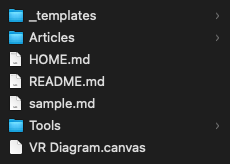
\includegraphics{assets/u1/vault-contents.png}

\end{figure}%

\begin{itemize}
\tightlist
\item
  Rename the folder to ldrs101-{[}firstname-lastname{]} (use all
  lowercase letters and a dash instead of spaces)
\item
  Open Obsidian and click the ``Open another vault'' icon in the bottom
  left corner
\end{itemize}

\begin{figure}[H]

\caption{\label{fig-image2}Screenshot of the Open Another Vault Button
in Obsidian}


\includegraphics{assets/u1/obsidian2.png}

\end{figure}%

\begin{itemize}
\tightlist
\item
  Choose the ldrs101-{[}firstame-lastname{]} folder, and then Obsidian
  will ask you to trust this vault
\item
  Click ``Trust author and enable plugins''
\item
  Once you are in the vault, feel free to take a look around---you will
  notice a Home page, a Tools folder with some files in it, and a VR
  Diagram Canvas
\end{itemize}

\end{tcolorbox}

Now that you have a place to record your course notes, let's jump back
into the discussion about digital literacy. Traditionally, literacy was
about speaking, listening, reading and writing. Literacy has taken on a
much broader and complex meaning. Today there's also digital literacy,
media literacy, new literacy, and so on. In the activity below you are
invited to reflect on how your literacies have changed when compared to
your parents, and to speculate on new literacies the next generation of
learners may need for the future.

\subsection{Activity: Reflection on the 21st Century
Learner}\label{activity-reflection-on-the-21st-century-learner}

\begin{tcolorbox}[enhanced jigsaw, toprule=.15mm, colback=white, colframe=quarto-callout-note-color-frame, bottomtitle=1mm, leftrule=.75mm, coltitle=black, titlerule=0mm, rightrule=.15mm, colbacktitle=quarto-callout-note-color!10!white, left=2mm, title={Learning Activity}, opacitybacktitle=0.6, opacityback=0, breakable, toptitle=1mm, arc=.35mm, bottomrule=.15mm]

\begin{itemize}
\tightlist
\item
  \textbf{Watch}: The following video by the MacArthur Foundation
  questions how digital media are changing the way young people learn,
  play, socialize, and participate in civic life. In it, John Seely
  Brown, a researcher with particular interests in radical innovation
  and digital culture, suggests that today's gaming oriented children
  want to be measured and feel that if they are not learning, it is not
  fun. How does this relate to how you feel about learning?
\end{itemize}

\href{https://www.youtube.com/watch?v=c0xa98cy-Rw}{Watch:
\emph{Rethinking Learning: The 21st Century Learner}}(2010)

\url{https://www.youtube-nocookie.com/embed/c0xa98cy-Rw}

While you watch the video think about:

\begin{itemize}
\item
  What ``literacy'' skills have you acquired when compared to your
  parents?
\item
  What ``literacy'' skills will be important for future learners in
  higher education?
\item
  \textbf{Reflect} on the following writing prompts:

  \begin{itemize}
  \tightlist
  \item
    My parents did not need to \ldots{}
  \item
    A new literacy I acquired is the ability to \ldots{}
  \item
    Higher education students of the future will need to \ldots{}
  \item
    \ldots{} is an important 21st century skill for future employment
  \end{itemize}
\item
  \textbf{Write}: To complete this activity, click ``Open Today's Daily
  Note'' in your Obsidian vault and write your reflections.
\end{itemize}

\begin{figure}[H]

\caption{\label{fig-tdn}Screenshot, Obsidian, Where to Find Today's
Daily Note (Icon Circled)}

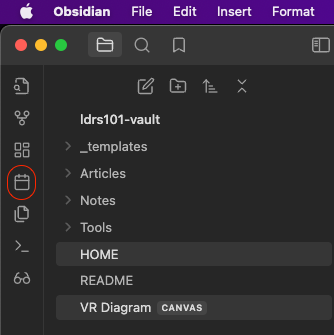
\includegraphics{assets/u1/tdn.png}

\end{figure}%

\begin{itemize}
\tightlist
\item
  Style your text using Markdown codes. Click here for the basic
  Markdown syntax (n.d.).
\item
  Feel free to add images and other media!
\end{itemize}

Please make sure you add tags to your note. Suggested tags might be
\#digital-literacy \#ldrs101 \#macarthur-foundation \#john-seely-brown.

Notice that tags start with a hashtag and contain no spaces. Separate
words with a hyphen.

\end{tcolorbox}

Let's dive a little deeper into this topic of digital literacy. What is
it? How would you define digital literacy?

In the next activity, you will start to unpack this term and prepare
your own initial definition of digital literacy.

\subsection{Activity: Defining Digital
Literacy}\label{activity-defining-digital-literacy}

\begin{tcolorbox}[enhanced jigsaw, toprule=.15mm, colback=white, colframe=quarto-callout-note-color-frame, bottomtitle=1mm, leftrule=.75mm, coltitle=black, titlerule=0mm, rightrule=.15mm, colbacktitle=quarto-callout-note-color!10!white, left=2mm, title={Learning Activity}, opacitybacktitle=0.6, opacityback=0, breakable, toptitle=1mm, arc=.35mm, bottomrule=.15mm]

Let's take a look at the definitions of digital literacy and digital
skills on the web and identify the difference. Follow the steps below
and feel free to jot down some notes in your Obsidian journal. If you
are completing this activity on a new day, create a new daily note.

\begin{itemize}
\tightlist
\item
  \textbf{Read}:

  \begin{itemize}
  \tightlist
  \item
    Read Wikipedia's definition (2024) of igital literacy---is this a
    good description?
  \item
    Scan the \#diglit or \#digital-literacy hashtags on
    \href{https://x.com/home}{X (Twitter)}---did you find any valuable
    links to defining digital literacy?
  \item
    Conduct a Google search for ``digital literacy.'' Select a few
    definitions you like and record their URLs, for example by adding
    these to your browser bookmarks.
  \item
    Conduct a Google search for ``digital skills.'' Select one or two
    definitions you like and record the URLs.
  \item
    Conduct a Google search for ``digital fluency.'' Select one or two
    definitions.
  \item
    What are the differences between digital literacies, digital
    fluency, and digital skills? How are these concepts related?
  \item
    Read \emph{What is Digital Literacy?} (2014) by POMO---is this a
    reliable source?
  \item
    How would you rate the academic quality of the definitions you found
    (e.g., low or high quality)?
  \item
    What did you discover?
  \end{itemize}
\item
  \textbf{Write}: Share your thoughts and experiences by posting on the
  LDRS 101 Discourse chat. For example:

  \begin{itemize}
  \tightlist
  \item
    The major difference between digital skills and literacies is
    \ldots{}
  \item
    I didn't realize that \ldots{}
  \item
    For me, digital literacy means \ldots''
  \end{itemize}
\end{itemize}

\end{tcolorbox}

\subsection{Digital Literacies and
Skills}\label{digital-literacies-and-skills}

Digital literacies for academic learning involves more than Facebook,
Snapchat, or X (Twitter) and the associated technical skills in using
these technologies.

As you explore the concept, you will find online resources which confuse
digital skills with digital literacies. The activities which follow aim
to provide an initial introduction to the wide range of digital
literacies associated with academic learning. We will explore the
concept of digital literacies in greater depth as we progress with the
course. When exploring these online resources we encourage you to
differentiate between skills and literacies, and to develop a critical
disposition. Digital literacies involve issues, norms, and habits of
mind surrounding technologies used for a particular purpose. However,
these literacies are closely related to technical proficiency in using a
range of digital applications.

\subsection{Activity: What Are Digital
Literacies?}\label{activity-what-are-digital-literacies}

\begin{tcolorbox}[enhanced jigsaw, toprule=.15mm, colback=white, colframe=quarto-callout-note-color-frame, bottomtitle=1mm, leftrule=.75mm, coltitle=black, titlerule=0mm, rightrule=.15mm, colbacktitle=quarto-callout-note-color!10!white, left=2mm, title={Learning Activity}, opacitybacktitle=0.6, opacityback=0, breakable, toptitle=1mm, arc=.35mm, bottomrule=.15mm]

Watch educator and researcher Doug Belshaw as he discusses his digital
literacies framework:

\begin{itemize}
\tightlist
\item
  \href{https://www.youtube.com/watch?v=A8yQPoTcZ78}{Watch: \emph{The
  Essential Elements Of Digital Literacies: Doug Belshaw At
  TedxWarwick}}(2012)
\end{itemize}

\url{https://www.youtube-nocookie.com/embed/A8yQPoTcZ78}

\begin{itemize}
\tightlist
\item
  \textbf{Read}: Next, read the
  \href{assets/u1/JISC_REPORT_Digital_Literacies_280714_PRINT.pdf}{\emph{Quick
  Guide - Developing Students' Digital Literacy}} (n.d.)
\end{itemize}

This guide defines digital literacies as ``the capabilities which fit an
individual for living, learning and working in a digital society (n.d.,
Introduction).'' Furthermore, this report distinguishes between seven
elements of digital literacies:

\begin{figure}[H]

\caption{\label{fig-image4}Career Ready Framework}

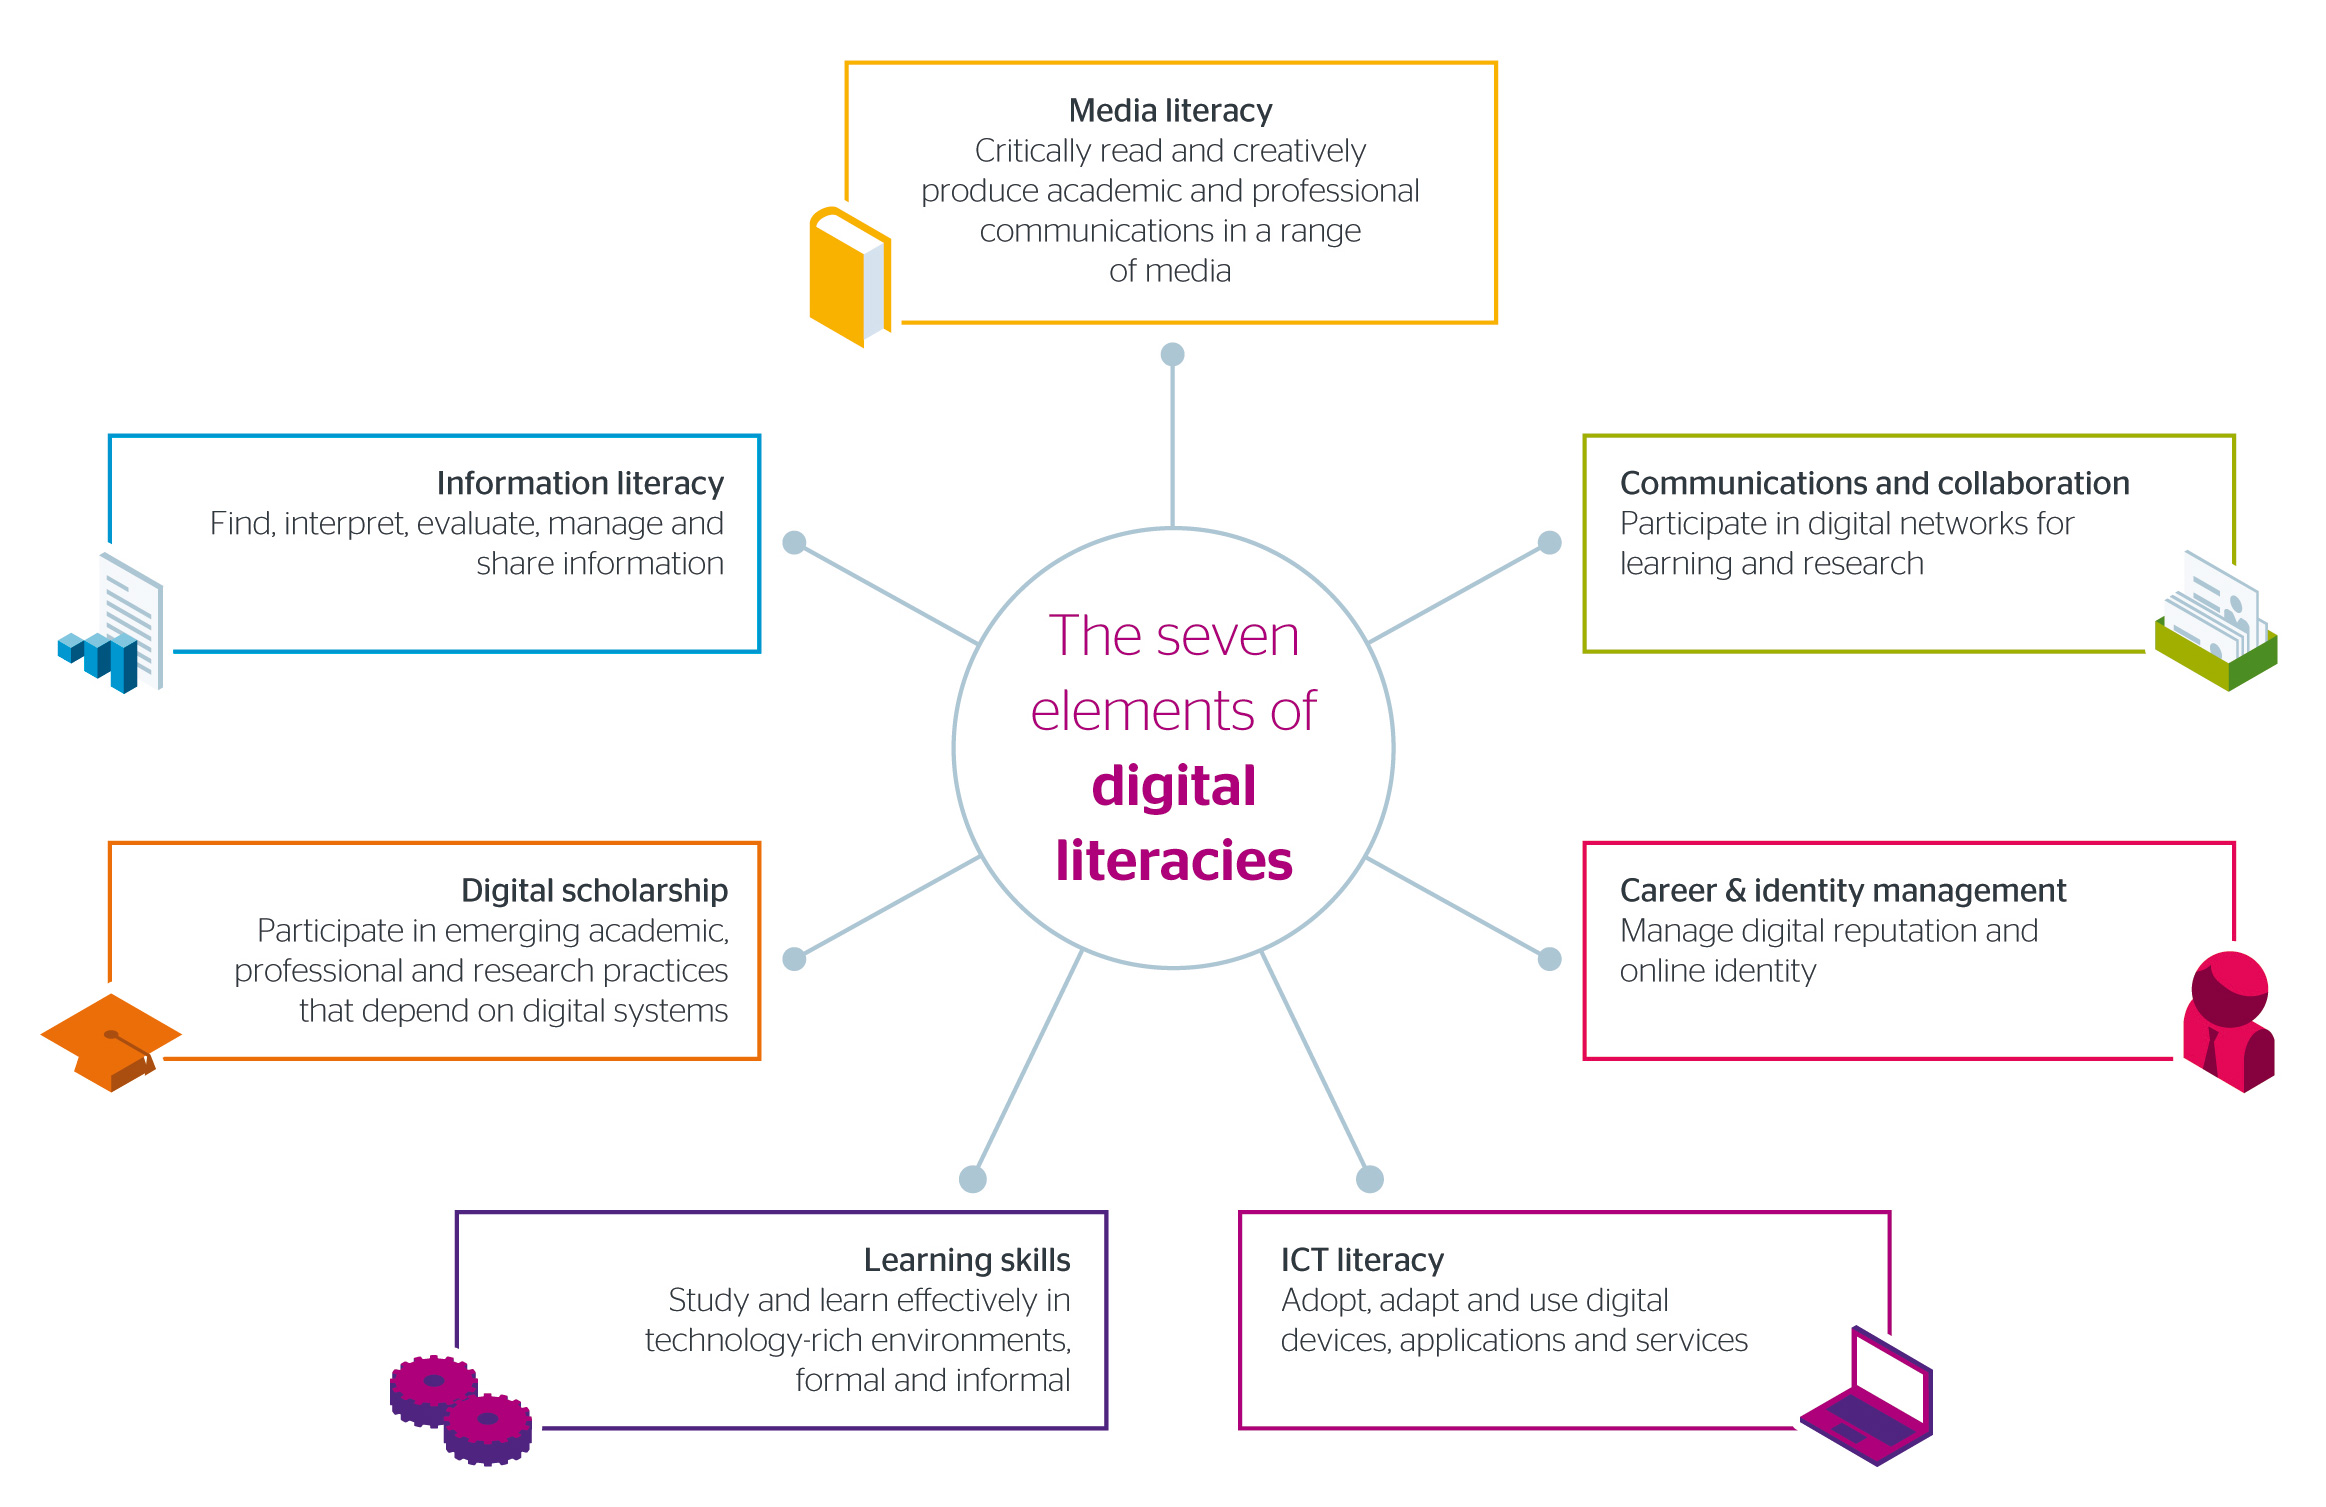
\includegraphics{assets/u1/7-digital-literacy-elements.png}

\end{figure}%

\begin{tcolorbox}[enhanced jigsaw, toprule=.15mm, colback=white, colframe=quarto-callout-note-color-frame, arc=.35mm, opacityback=0, breakable, rightrule=.15mm, bottomrule=.15mm, leftrule=.75mm, left=2mm]

\emph{Note.} From
``\href{https://digitalcapability.jiscinvolve.org/wp/files/2014/09/JISC_REPORT_Digital_Literacies_280714_PRINT.pdf}{\emph{Quick
Guide - Developing Students' Digital Literacy}},'' by Jisc Digital
Experience Insights, n.d., p.~2, .
\href{https://creativecommons.org/licenses/by-nc-nd/2.0/uk/}{CC BY-NC-ND
2.0 UK}.

\end{tcolorbox}

Do you agree that these are the key literacies you need to live, learn,
and work in today's society? What would you add?

Conduct a quick Google search for ``digital literacies'' and add in
terms such as ``essential,'' ``top,'' ``21st century.'' What other
literacies or skills are emphasized? What would your list be for digital
literacies that are important for you?

\end{tcolorbox}

\subsection{Activity: Why Digital Literacy
Matters}\label{activity-why-digital-literacy-matters}

\begin{tcolorbox}[enhanced jigsaw, toprule=.15mm, colback=white, colframe=quarto-callout-note-color-frame, bottomtitle=1mm, leftrule=.75mm, coltitle=black, titlerule=0mm, rightrule=.15mm, colbacktitle=quarto-callout-note-color!10!white, left=2mm, title={Learning Activity}, opacitybacktitle=0.6, opacityback=0, breakable, toptitle=1mm, arc=.35mm, bottomrule=.15mm]

A key component of digital literacy and networked learning relates to
the ability to engage meaningfully in online learning communities.

This learning activity will provide you with another opportunity to
connect with your peers in Discourse and contribute to online learning
discussions.

Watch the following video and jot down the reasons why digital literacy
matters to you, then complete the steps which follow.

\begin{itemize}
\tightlist
\item
  \href{https://www.youtube.com/watch?v=p2k3C-iB88w}{Watch:
  \emph{Digital Literacy and Why it Matters} (2014)}
\end{itemize}

\url{https://www.youtube-nocookie.com/embed/p2k3C-iB88w}

\begin{itemize}
\tightlist
\item
  \textbf{Write}:

  \begin{itemize}
  \tightlist
  \item
    Go to the LDRS 101 section in Discourse
  \item
    Post a contribution to the discussion on digital literacies and why
    they are important for you
  \item
    Post one or two replies to interesting contributions (you should
    also ``like'' good contributions, use the person's username when
    replying, and if appropriate, quote a reply when responding.)
  \end{itemize}
\end{itemize}

\end{tcolorbox}

\subsection{Activity: Am I Digitally
Literate?}\label{activity-am-i-digitally-literate}

\begin{tcolorbox}[enhanced jigsaw, toprule=.15mm, colback=white, colframe=quarto-callout-note-color-frame, bottomtitle=1mm, leftrule=.75mm, coltitle=black, titlerule=0mm, rightrule=.15mm, colbacktitle=quarto-callout-note-color!10!white, left=2mm, title={Learning Activity}, opacitybacktitle=0.6, opacityback=0, breakable, toptitle=1mm, arc=.35mm, bottomrule=.15mm]

Digital literacy encompasses a wide range of capabilities which extend
beyond the digital skills associated with different technologies.
Consider the digital literacies you identified from the previous
activity.

\begin{itemize}
\tightlist
\item
  \textbf{Write}: Jot down one or more technologies or tools you would
  recommend for each of the skills and assess your competence in using
  each particular technology or tool (e.g., below average, average,
  above average, or excellent).
\item
  \textbf{Search}: Next, use your searching skills to discover online
  tests for assessing your digital literacies (don't spend more than 15
  to 20 minutes on the self-assessment activity).

  \begin{itemize}
  \tightlist
  \item
    Conduct a Google search using ``digital literacy self-assessment''
  \item
    Choose a link to conduct a self-assessment of your digital literacy
  \end{itemize}
\end{itemize}

Alternatively, you can choose from these resources:

\begin{itemize}
\item
  Take the Digital Literacy Self-Assessment (n.d.) from the Canadian
  Association for Supported Employment \textbf{or}
\item
  Use the
  \href{https://thinkspace.csu.edu.au/digitalcitizenshipguideetl523/}{Digital
  Literacy Self-Assessment Tool} (2020) from the Digital Citizenship
  Guide \textbf{or}
\item
  Explore the \emph{What is Digital Literacy?} page of the Digital
  Literacies Toolkit (n.d.) developed by the University of Southampton.
\item
  \textbf{Questions to Consider}:

  \begin{itemize}
  \tightlist
  \item
    Did the self-assessment you chose focus on digital skills or digital
    literacies?
  \item
    What did you learn from this exercise?
  \end{itemize}
\end{itemize}

Share your thoughts by posting on Discourse.

\end{tcolorbox}

\subsection{Visitors and Residents}\label{visitors-and-residents}

One way to start thinking about digital literacy is to create a map of
the apps and tools that you use, how you use them, and what traces of
your presence you leave behind on the web. We call this a Visitors and
Residents Diagram. To complete this activity, we'll first discuss some
key concepts.

Have you encountered the terms ``digital natives'' and ``digital
immigrants?'' What are your initial thoughts on their definitions?

\begin{tcolorbox}[enhanced jigsaw, toprule=.15mm, colback=white, colframe=quarto-callout-note-color-frame, arc=.35mm, opacityback=0, breakable, rightrule=.15mm, bottomrule=.15mm, leftrule=.75mm, left=2mm]
\begin{minipage}[t]{5.5mm}
\textcolor{quarto-callout-note-color}{\faInfo}
\end{minipage}%
\begin{minipage}[t]{\textwidth - 5.5mm}

Note: \href{https://marcprensky.com/}{Marc Prensky} coined the terms
``digital natives'' and ``digital immigrants.'' We recognize that the
term ``native'' should not be used to talk about people.

\end{minipage}%
\end{tcolorbox}

The essential argument is that certain generations have changed, in that
they have an innate ability to use and learn technology because they
have grown up using technology, and those generations whose formative
years pre-date the advent of the internet are forever at a disadvantage
compared to \emph{kids}. You can read a bit more about the idea on
Wikipedia, linked below. There is also a link in that article to
Prensky's original article.

Digital native

Aside from the problematic framing of learners as kids, there are some
distinct challenges with the idea of digital literacy being a fixed
trait rather than a matter of comfort, familiarity, and a skill that can
be practiced and learned. It is no secret that young people are
comfortable using social media apps such as TikTok, Instagram, SnapChat,
Weibo, WeChat, and the like, but this doesn't imply a superior aptitude
for learning technology compared to older generations, or an inherent
proficiency in doing so. For example, are most first-year university
students proficient in using a spreadsheet to create a budget? If they
have created a budget, it's more likely they use an app than a
spreadsheet.

We'd like to introduce you to a different way to conceptualize your
relationship with digital media, and that is that you may be a
\emph{visitor} in some web spaces and a \emph{resident} in others.
Places on the web where you might be a visitor are those places where
you quite literally visit, but importantly, don't leave a public trace
of your time there. You don't spend any time interacting with people,
but rather, you take a rather utilitarian approach by visiting a site,
doing a thing, and leaving.

Alternately, there are places and spaces on the web where \emph{you}
reside as a persona, where you interact, socialize, and leave traces of
yourself online. For some, that may be Facebook or Instagram, where you
keep in touch with friends and family, or X (formerly Twitter), or maybe
it's a blog, or social site. The important distinction is that these are
places where you connect with other people, where you are socially
\emph{present}.

At the same time, if we can imagine the visitor \(\leftrightarrow\)
resident continuum on a horizontal axis, there is also a personal
\(\updownarrow\) professional (or educational) continuum on a vertical
axis, leading to four quadrants where you might situate your technology
use.

\subsection{Activity: Where Am I
Online?}\label{activity-where-am-i-online}

\begin{tcolorbox}[enhanced jigsaw, toprule=.15mm, colback=white, colframe=quarto-callout-note-color-frame, bottomtitle=1mm, leftrule=.75mm, coltitle=black, titlerule=0mm, rightrule=.15mm, colbacktitle=quarto-callout-note-color!10!white, left=2mm, title={Learning Activity}, opacitybacktitle=0.6, opacityback=0, breakable, toptitle=1mm, arc=.35mm, bottomrule=.15mm]

The video below explains a process to help you think about where you
reside on the web.

\begin{itemize}
\tightlist
\item
  \href{https://www.youtube.com/watch?v=sPOG3iThmRI}{Watch:
  \emph{Visitors and Residents}(2014)}
\end{itemize}

\url{https://www.youtube-nocookie.com/embed/sPOG3iThmRI}

\begin{itemize}
\tightlist
\item
  \textbf{Questions to Consider:}
\item
  What surprised you as you watched the video?
\item
  How can you apply the concepts presented to your experience in
  learning with technology?
\end{itemize}

Feel free to jot down your notes in Obsidian.

\end{tcolorbox}

Now to the task of creating your own Visitors and Residents Diagram.

See the diagram below \ldots{} keep in mind that this diagram represents
a set of tools that its creator has been using for a decade or more, and
that they have invested their career in educational technology. There is
a lot here; yours might look significantly different with only a few
tools here and there. Or perhaps your diagram has a plethora of tools
you use regularly. The key idea of visitors and residents is for you to
think about which technologies you use as a resident, and then to think
about which tools you may have tried or are interested in pursuing. From
there, we can begin to plan for tools we can use that afford us the
opportunity to reside there.

\begin{figure}

\caption{\label{fig-vrxdiagramx2}Visitor--Resident Diagram}

\includegraphics{assets/u1/vr-diagram-2.png}

\end{figure}%

It is certainly notable that this diagram's creator is very much a
visitor in Moodle! This does not mean that they don't spend much time
there, they spend a significant portion of every day working in Moodle,
rather, the work that they do there leaves very little trace of their
personality. You will (hopefully) see Moodle as much more of a place
where you reside. But this foregrounds the question of whether Moodle is
actually designed to promote residencies. Certainly the forums allow for
users to project their persona into the system, as do a few of the other
features, but the system itself is very heavily templated. There are
profiles that can be edited, but users are limited to one very tiny
image, and virtually no opportunity to determine for themselves what
they want to share. There is little room for customization, and every
time a course ends every single user must recreate their persona in a
new course site (or five).

For many university students, a Learning Management System (LMS) like
Moodle is a perfectly reasonable place to reside and they feel
comfortable accessing course materials, finding their grades,
communicating with classmates, and so on. And just like our physical
homes, the quality of the community that lives there isn't determined by
the features of the house itself, but by the people who share the space
and how they structure their time and interactions.

\subsection{Activity: Visitor and Resident
Diagram}\label{activity-visitor-and-resident-diagram}

\begin{tcolorbox}[enhanced jigsaw, toprule=.15mm, colback=white, colframe=quarto-callout-note-color-frame, bottomtitle=1mm, leftrule=.75mm, coltitle=black, titlerule=0mm, rightrule=.15mm, colbacktitle=quarto-callout-note-color!10!white, left=2mm, title={Learning Activity}, opacitybacktitle=0.6, opacityback=0, breakable, toptitle=1mm, arc=.35mm, bottomrule=.15mm]

This activity will help you think about how the tools we use shape and
sometimes determine the nature of our interactions with each other. Do
the tools you use fall on the visitor or the resident end of your
continuum? How do these tools impact your learning?

\begin{itemize}
\tightlist
\item
  \textbf{Read:}
  \href{https://firstmonday.org/ojs/index.php/fm/article/view/3171}{\emph{Visitors
  and Residents: A New Typology for Online Engagement} (2011)}
\item
  \textbf{Create} a new canvas in your Obsidian vault and create your
  own Visitor--Resident Diagram. We have created a sample diagram in the
  vault.
\end{itemize}

\begin{tcolorbox}[enhanced jigsaw, toprule=.15mm, colback=white, colframe=quarto-callout-note-color-frame, arc=.35mm, opacityback=0, breakable, rightrule=.15mm, bottomrule=.15mm, leftrule=.75mm, left=2mm]

This diagram can be used to demonstrate your understanding of the course
learning outcomes. See the Assessment tab in Moodle for how this
activity relates to the assessments in this course\emph{.}

\end{tcolorbox}

\end{tcolorbox}

\section{Digital Privacy and Safety}\label{digital-privacy-and-safety}

Now that you have assessed some of your digital skills or literacies,
let's focus our attention on privacy and safety. In this section we
summarize important practices as a reminder to remain vigilant in
protecting your privacy and security online. If you are unsure about
good security practices, there are a wealth of online resources you can
(and should) consult.

\subsubsection*{Privacy}\label{privacy}
\addcontentsline{toc}{subsubsection}{Privacy}

Your privacy is fragile, easy to lose instantaneously, and difficult to
retrieve in an environment that requires so much online interaction.

\begin{itemize}
\tightlist
\item
  \href{https://en.wikipedia.org/wiki/Identity_theft}{\textbf{Identity
  theft}} happens, frequently.

  \begin{itemize}
  \tightlist
  \item
    Never put your social insurance number, your birthday, your mother's
    maiden name, or any other personal facts anywhere online. Everyone
    on the internet will be able to access this information.
  \item
    Always assume that anything you write online (including email) can,
    and probably will, eventually leak. Keep your email address
    private---to avoid receiving spam. If your email is published in a
    plain form anywhere online, even if it is part of an archived email
    list, spammers will ``harvest'' it for their databases.
  \end{itemize}
\item
  \textbf{Spam email
  \href{https://securelist.com/spam-report-2019/96527/}{(at least half
  of all email being sent)}} is an unfortunate fact of our modern lives.

  \begin{itemize}
  \tightlist
  \item
    If you must publish your email address online, consider creating a
    ``sacrificial'' email address, or one you only use to publish
    online. You can create an email ``alias'' which you can set to
    automatically forward to your primary email, and easily disable if
    your spam volumes increases. Many email services will automatically
    generate random email addresses that you can use to hide your true
    address.
  \item
    Another approach is to avoid publishing the email address as
    something like \emph{mailto:myname@somewebdomain.net}. Instead, you
    might use more confusing text, such as myname-at-somewebdomain-net.
    Some websites support using these types of obfuscation methods, but
    the spammers who ``scrape'' email addresses from websites to
    populate their spam databases use increasingly sophisticated methods
    to defeat these methods.
  \item
    Basically, avoid publishing the email addresses you value online to
    decrease the amount of spam you receive.
  \end{itemize}
\end{itemize}

\subsubsection*{Passwords}\label{passwords}
\addcontentsline{toc}{subsubsection}{Passwords}

What about passwords? Many people have just one, or maybe a few. Given
the number of websites and web services which require password-based
authentication, this is not good enough to avoid an identity disaster.

The problem with having only a few passwords is that even resource-rich
and security-critical organizations have
\href{https://gizmodo.com.au/2017/05/over-560-million-passwords-discovered-in-anonymous-online-database/}{suffered
massive leaks}. If even one of them suffers a data leak, identity
thieves will obtain your password and try to use it on other websites.
It is easy for them to do this using computer technologies.

Other ways someone can get your password include:

\begin{itemize}
\tightlist
\item
  Sniffing traffic when you log in to a nonsecure website that uses
  http:// rather than https:// (the ``s'' stands for secure because your
  data transmission's encrypted). Look for the Lock icon.png in your
  address bar.
\item
  Sniffing emails---your email, unless encrypted, is not secure. Never
  send a login and password along with the web address of a service
  (similarly, don't send credit card numbers).
\item
  Phishing attacks---where someone sends you an email that looks like it
  is from a trusted sender, such as from a friend, your bank, an online
  store you frequent, or a government agency, and asks you to enter your
  password to confirm it. No one should ever ask you to enter your
  password via email.
\item
  Always check the web address (hover over the link) to make sure it
  corresponds to the right place or call the sender to confirm the
  request over the phone.
\item
  Brute force---hackers often use computers to guess your password,
  beginning with a list of common passwords, and try different
  combinations until they get it right, or until the system locks them
  out for trying too many times.
\item
  ``How secure is my password'' sites---you should avoid these sites and
  never type your password into a website or email response that is not
  appropriate, especially when you know the sender also knows your
  email.
\item
  Once your email and any password combination are known, identity
  thieves will try to use them at various websites, because they know
  most people only use a few passwords. A thief who discovers a password
  you created for a website you rarely use will try to compromise the
  security of a website that is important to you such as your email
  system, your workplace, social media accounts, or bank account.
\end{itemize}

Here is a table that shows how quickly passwords can be cracked using
brute force methods. Note that the best passwords are both long and
include a mix of numbers, lowercase and uppercase letters, and symbols.

\begin{figure}

\caption{\label{fig-brute}Time Needed to Crack Passwords of Varying
Complexity in a Brute Force Attack.}

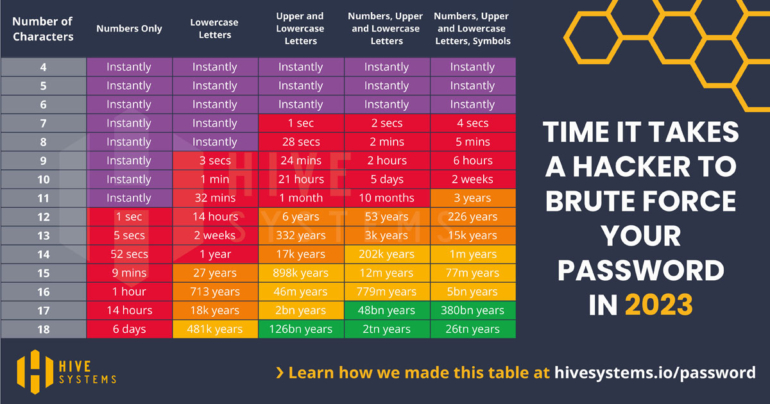
\includegraphics{assets/u1/brute.jpg}

\end{figure}%

\begin{tcolorbox}[enhanced jigsaw, toprule=.15mm, colback=white, colframe=quarto-callout-note-color-frame, arc=.35mm, opacityback=0, breakable, rightrule=.15mm, bottomrule=.15mm, leftrule=.75mm, left=2mm]

\emph{Note}. From ``Are Your Passwords in the Green in 2023?,'' by C.
Nesky, 2023, \emph{Hive Systems}
(https://www.hivesystems.com/blog/are-your-passwords-in-the-green-2023).
Copyright 2024 \href{https://www.hivesystems.com/}{Hive Systems}.
Reprinted with permission.

\end{tcolorbox}

There are services you can use to check if your email is part of a
leaked password data set. So, what can you do to protect yourself?

\subsubsection*{Password Managers}\label{password-managers}
\addcontentsline{toc}{subsubsection}{Password Managers}

Get a \href{https://en.wikipedia.org/wiki/Password_manager}{password
manager}. They are incredibly helpful and convenient now that many of us
use several computers and mobile devices. Password managers help you
manage your passwords.

\begin{itemize}
\tightlist
\item
  When you choose a password manager make sure you create one
  \href{https://www.howtogeek.com/195430/how-to-create-a-strong-password-and-remember-it/}{strong
  password}, such as a full sentence with some numbers and special
  characters. This is all you need to remember---the password manager
  remembers the others. The ensures you generate a different, fully
  random password for each website you use that requires a password.
\item
  Good password managers only ever store your details in an encrypted
  form, where even the company that stores it cannot see your passwords.
  To access your passwords, you log into the password manager service
  using your single, strong password (via a secure web link---usually
  the default, but always check!).
\item
  There are many
  \href{https://www.google.co.nz/search?q=password+managers&bshm=rimc/1}{password
  manager options}. Some widely used proprietary options include
  \href{https://www.lastpass.com/}{Lastpass} and
  \href{https://1password.com/}{1password}. Open source options also
  exist, such as \href{https://bitwarden.com/}{Bitwarden}. Sadly, some
  of the most popular password managers have suffered from software bugs
  that have exposed user passwords.
\end{itemize}

\subsection{Activity: Get a Password
Manager}\label{activity-get-a-password-manager}

\begin{tcolorbox}[enhanced jigsaw, toprule=.15mm, colback=white, colframe=quarto-callout-note-color-frame, bottomtitle=1mm, leftrule=.75mm, coltitle=black, titlerule=0mm, rightrule=.15mm, colbacktitle=quarto-callout-note-color!10!white, left=2mm, title={Learning Activity}, opacitybacktitle=0.6, opacityback=0, breakable, toptitle=1mm, arc=.35mm, bottomrule=.15mm]

If you don't already use a password manager, set up an account with
\href{https://www.lastpass.com/}{Lastpass},
\href{https://1password.com/}{1password}, or the free password manager,
\href{https://bitwarden.com/}{Bitwarden} to familiarize yourself with
how password managers work.

\begin{itemize}
\tightlist
\item
  \textbf{Read}: \emph{How to Start Using a Password Manager} (2021).

  \begin{itemize}
  \tightlist
  \item
    Create an account on the password manager site and establish a
    master password (conduct an online search for advice on choosing a
    secure master password).
  \item
    Install the browser extension for your local browser.
  \item
    Choose one of the TWU course websites and set up a new secure
    password using your password manager.
  \item
    Log out of the TWU course website and log in again using the
    password manager.
  \item
    Install the mobile phone app for your operating system, and desktop
    application for your computer (if this applies). Synchronize the
    local app with your online vault.
  \item
    Consider using the password manager for your online accounts so you
    can easily set up and maintain a unique password for each online
    account you use.
  \end{itemize}
\end{itemize}

\end{tcolorbox}

\subsubsection*{\texorpdfstring{\emph{Good Messaging
Hygiene}}{Good Messaging Hygiene}}\label{good-messaging-hygiene}
\addcontentsline{toc}{subsubsection}{\emph{Good Messaging Hygiene}}

Always assume that anyone can and will read anything you write in an
email. Email is not a secure form of communication. Few people encrypt
their email because it is an extra step that even the most technically
inclined users are reluctant to take. Both sender and recipient have to
be technically proficient.

Text messages and instant messaging programs such as Facebook Messenger
are also insecure. Anyone, including government officials and the
organization that runs the service, such as Facebook employees, can read
it.

\subsubsection*{Secure Your Own Privacy}\label{secure-your-own-privacy}
\addcontentsline{toc}{subsubsection}{Secure Your Own Privacy}

Never send any sensitive data such as your social insurance number,
credit card number, password, or other personal information via email or
text. Call the person to provide this information over the phone.

You can use a secure, encrypted text message service such as Signal if
necessary. It is available at no cost, works on most platforms, and
encrypts text messages on your phone. If you text someone else with
Signal installed, the entire transaction is encrypted.

\subsubsection*{Secure the Privacy of
Others}\label{secure-the-privacy-of-others}
\addcontentsline{toc}{subsubsection}{Secure the Privacy of Others}

Another element of good digital hygiene is to protect the identity of
others. For example, never send group emails using To: or CC: (carbon
copy) for each email address. You will reveal the email addresses for
everyone on your list. This is especially problematic if you or another
person saves the email message and displays it on the web, such as in a
mailing list archive. This makes it easy for spammers and hackers to
access and download all of those email addresses.

Use BCC: (blind carbon copy), to hide the email addresses from your
recipients to protect everyone's privacy. Use your own email address,
and BCC the rest of the recipients, if your email software requires you
to insert an email address into the To: box.

When using an email mailing list where you send messages to a single
email address to a list of people, never CC: someone else in the same
message. This will compromise the privacy of every CC'd recipient and
the privacy of the list. Always check with the people on the list to
ensure you are not taking unacceptable liberties.

If someone asks you to share an email address of a friend or colleague
you should ask permission to share their email address, and state why
the third party is requesting their email.

\subsubsection*{Be a Thoughtful Sceptic}\label{be-a-thoughtful-sceptic}
\addcontentsline{toc}{subsubsection}{Be a Thoughtful Sceptic}

So how can we protect ourselves if new threats are emerging all the
time?

\begin{itemize}
\tightlist
\item
  Be conscious of where you put information that is ``private'' to you.
\item
  Beware of the terms of service (ToS) of social media providers such as
  Facebook. Use a service such as \href{https://tosdr.org/}{\emph{Terms
  of Service: Didn't Read} (TOSDR)} to help identify risky, overreaching
  services. You may be able to use certain privacy settings to protect
  your information.
\item
  Always check the identity of a website before you enter any passwords
  or personal information. Secure certificates are generally trustworthy
  but be sure to check the names and details.
\item
  Always ask whether you should trust a provider or a government agency.
  Always ask ``who benefits when I do this?'' What are their incentives?
\item
  Protect your own data and be even more protective of others' private
  information. For example, be cautious before posting information about
  yourself or someone else. Be especially cautious when posting pictures
  or videos of their children.
\item
  Remember, complacency and unwarranted trust are your biggest enemies.
  A healthy paranoia is good for your digital health. Think about the
  great amount of time and effort it will take to regain your identity
  (and credit rating) if your information is compromised.
\end{itemize}

\subsection{Activity: Tos Analysis}\label{activity-tos-analysis}

\begin{tcolorbox}[enhanced jigsaw, toprule=.15mm, colback=white, colframe=quarto-callout-note-color-frame, bottomtitle=1mm, leftrule=.75mm, coltitle=black, titlerule=0mm, rightrule=.15mm, colbacktitle=quarto-callout-note-color!10!white, left=2mm, title={Learning Activity}, opacitybacktitle=0.6, opacityback=0, breakable, toptitle=1mm, arc=.35mm, bottomrule=.15mm]

\begin{itemize}
\tightlist
\item
  \textbf{Identify}: Use the \href{https://tosdr.org/}{\emph{Terms of
  Service: Didn't Read}} (n.d.) site to look up each of the apps we will
  learn in this course. Each tool currently has its own file in your
  Obsidian vault with a template ready to go for you. Fill out the
  template for each tool based on what is available on tosdr.org and
  your own examination of the ToS for each tool.
\end{itemize}

Feel free to add components to the template.

\end{tcolorbox}

\subsection{Activity: Introduction To Reflective
Journaling}\label{activity-introduction-to-reflective-journaling}

\begin{tcolorbox}[enhanced jigsaw, toprule=.15mm, colback=white, colframe=quarto-callout-note-color-frame, bottomtitle=1mm, leftrule=.75mm, coltitle=black, titlerule=0mm, rightrule=.15mm, colbacktitle=quarto-callout-note-color!10!white, left=2mm, title={Learning Activity}, opacitybacktitle=0.6, opacityback=0, breakable, toptitle=1mm, arc=.35mm, bottomrule=.15mm]

For the final activity of Unit 1 you will be asked to write a reflective
journal entry in Obsidian on the topic of digital literacy. This entry
can be used as part of \textbf{Assignment 1: Reflective Journal}.

Prior to completing this activity, let's discuss the practice of writing
in a Reflective Journal.

A reflective journal is simply a record of your thoughts. It is a
reflection of the way you think and the manner in which you respond to
your learning. Journals can consist of traditional note taking, mind
maps, pictures, stream-of-consciousness writing, recordings, quotes,
sketches, or drawings---whatever you choose to include. Experiment and
have fun. The purpose of journaling is to make you an active participant
in your learning experiences as you engage in the various activities
throughout the course's readings, activities, and discussions.
Reflecting upon these learning events will help you gain a deeper
understanding of the course materials and help integrate your learning
into applied practice in your everyday life and work. Throughout the
course, we will remind you to write in your journal, as we want to be
sure you are actively learning the material. To assist you, we have
provided you with questions you can ask yourself in order to get your
creative energies flowing. Reflective journaling is an activity you can
and should complete on a regular or daily basis, even beyond the
prompting in course activities.

\href{https://www.youtube.com/watch?v=QoI67VeE3ds}{Watch:
\emph{Reflective Writing}(2014)}

\url{https://www.youtube-nocookie.com/embed/QoI67VeE3ds}

Here are some common questions used for reflective journaling. As you
read them, consider what you have learned in this first unit.

\begin{itemize}
\tightlist
\item
  In your view, what were the most important points in the readings or
  activities?
\item
  What information did you already know? What skills did you already
  have?
\item
  What new knowledge, skills, or perspectives have you gained?
\item
  What information was easy to remember or learn? Why?
\item
  What concepts or skills did you find more difficult? Why?
\item
  How can you apply this knowledge to your studies or future career?
\item
  How has this knowledge helped you to make sense of your current or
  previous experience?
\item
  Has your understanding of a personal or work-related situation changed
  after studying these concepts?
\item
  Did you agree or disagree with any of the material? If yes, how did
  you react and why?
\item
  If you could have the opportunity to engage in further learning, what
  would it be?
\item
  What further questions would like to ask about the concepts presented
  in this unit?
\item
  What other concepts, resources or discussions would be of interest?
\end{itemize}

\end{tcolorbox}

\subsection{Activity: Digital Literacies for Online
Learning}\label{activity-digital-literacies-for-online-learning}

\begin{tcolorbox}[enhanced jigsaw, toprule=.15mm, colback=white, colframe=quarto-callout-note-color-frame, bottomtitle=1mm, leftrule=.75mm, coltitle=black, titlerule=0mm, rightrule=.15mm, colbacktitle=quarto-callout-note-color!10!white, left=2mm, title={Learning Activity}, opacitybacktitle=0.6, opacityback=0, breakable, toptitle=1mm, arc=.35mm, bottomrule=.15mm]

\begin{itemize}
\tightlist
\item
  \textbf{Write}: In this activity you are asked to write a reflective
  journal entry on the topic of digital literacy.
\end{itemize}

First, let's get you set up in Obsidian. Click the little calendar icon
in the sidebar of Obsidian to open today's daily note.

\begin{figure}[H]

\caption{\label{fig-obsidian1}Screenshot of the Daily Note Icon in
Obsidian (Circled)}

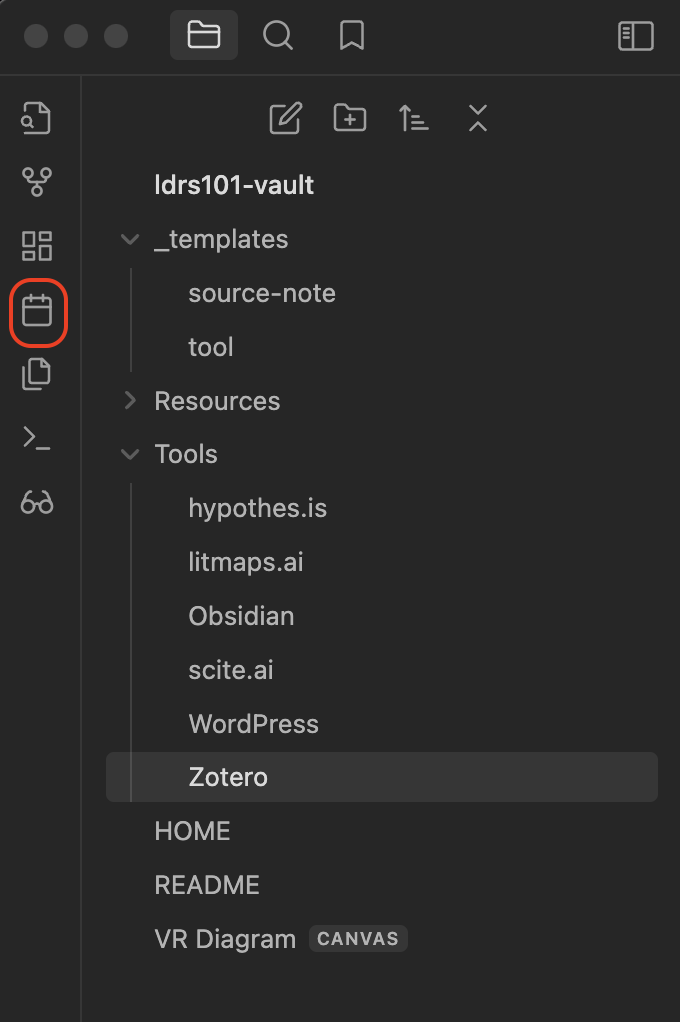
\includegraphics{assets/u1/obsidian1.png}

\end{figure}%

Next, respond to the following prompts:

\begin{itemize}
\tightlist
\item
  Write your personal definition of digital literacies justified from
  your reading of the literature (about 100 to 150 words).
\item
  Describe what digital literacies mean for you in a sentence.
\item
  Create a link to your VR diagram map in your entry.
\item
  Summarize an action plan for improving your digital
  literacies---identify the literacies you plan to improve including the
  reasons why and how you aim to achieve this.
\item
  Ensure that your references are cited appropriately.
\end{itemize}

\begin{tcolorbox}[enhanced jigsaw, toprule=.15mm, colback=white, colframe=quarto-callout-note-color-frame, arc=.35mm, opacityback=0, breakable, rightrule=.15mm, bottomrule=.15mm, leftrule=.75mm, left=2mm]

\emph{This journal entry can be used to demonstrate your understanding
of the course learning outcomes. See the Assessment tab in Moodle for
how this activity relates to the assessments in this course.}

\end{tcolorbox}

\end{tcolorbox}

\section*{Summary}\label{summary}
\addcontentsline{toc}{section}{Summary}

\markright{Summary}

In this first unit, you have had the opportunity to learn about some of
the impacts of ``the digital\emph{``} on your life. You have started to
build an academic knowledge management workflow, a pivotal skill
essential for efficiently organizing, accessing, and leveraging
information. Throughout the unit, you've actively engaged with digital
tools, shared insights into your personal interactions with digital
technology, and begun applying these tools to enhance your academic
learning experience. Furthermore, you've developed a personalized
understanding of digital literacy and explored how to protect yourself
and others in digital and online contexts. As you progress through the
course, take a moment to identify the specific literacies you aspire to
refine and articulate the concrete steps you intend to take in pursuit
of these goals.

\begin{tcolorbox}[enhanced jigsaw, toprule=.15mm, colback=white, colframe=quarto-callout-note-color-frame, bottomtitle=1mm, leftrule=.75mm, coltitle=black, titlerule=0mm, rightrule=.15mm, colbacktitle=quarto-callout-note-color!10!white, left=2mm, title={Checking Your Learning}, opacitybacktitle=0.6, opacityback=0, breakable, toptitle=1mm, arc=.35mm, bottomrule=.15mm]

Before you move on to the next unit you may want to check that you are
able to:

\begin{itemize}
\tightlist
\item
  Explore common digital tools used at Trinity Western University
\item
  Describe your engagement with digital technology
\item
  Apply digital tools to support learning in an academic environment
\item
  Explain what digital literacy means to you
\item
  Examine privacy concerns related to various platforms and tools
\item
  Describe how to protect yourself and others in the digital environment
\item
  Identify the literacies you plan to improve and what steps you will
  take to achieve your goals
\end{itemize}

\end{tcolorbox}

\bookmarksetup{startatroot}

\chapter{Discovering and Curating
Resources}\label{discovering-and-curating-resources}

\section*{Overview}\label{overview-1}
\addcontentsline{toc}{section}{Overview}

\markright{Overview}

In this module, we'll dive into three important aspects of utilizing
digital resources effectively. Firstly, we'll explore the art of
discovering and selecting valuable resources for your academic and
professional needs. You'll learn how to search efficiently, critically
assess sources for credibility and relevance, and finetune your search
techniques.

Next, we'll delve into the world of citation management. Properly citing
your sources is vital in academic writing to avoid plagiarism, and we'll
introduce you to various citation styles such as APA, MLA, and Chicago.
You'll also gain practical experience with citation management tools to
help streamline the citation process and manage your references
efficiently.

Finally, we'll discuss the concept of openness in education. We'll
explore open educational resources (OER), the benefits and challenges of
open access, and the role of Creative Commons licenses in educational
materials. This discussion will open your eyes to the changing landscape
of educational resources and the ethics surrounding them. Throughout
these topics, you'll engage in hands on activities, group projects, and
discussions to enhance your critical thinking skills and promote
responsible use of digital resources.

\subsection*{Topics}\label{topics-1}
\addcontentsline{toc}{subsection}{Topics}

This unit is divided into the following topics:

\begin{enumerate}
\def\labelenumi{\arabic{enumi}.}
\tightlist
\item
  Finding and selecting resources
\item
  Evaluating resources
\item
  Citation management
\item
  Openness in education
\end{enumerate}

\subsection*{Learning Outcomes}\label{learning-outcomes}
\addcontentsline{toc}{subsection}{Learning Outcomes}

When you have completed this unit you will be able to:

\begin{itemize}
\tightlist
\item
  Develop effective search strategies to locate scholarly resources
  using various academic databases and online repositories
\item
  Apply strategies to assess, analyze, and evaluate the reliability of
  resources, including reporting in the mass media
\item
  Utilize citation management tools effectively to organize references,
  generate bibliographies, and streamline the citation process
\item
  Describe the principles of openness in education, including open
  educational resources (OER), and open access
\item
  Build and customize technology integrated workflows to enhance and
  enrich your learning journey
\item
  Apply digital literacy skills to evaluate the legitimacy, credibility,
  and reliability of online resources for academic study
\end{itemize}

\subsection*{Activity Checklist}\label{activity-checklist-1}
\addcontentsline{toc}{subsection}{Activity Checklist}

Here is a checklist of learning activities you will benefit from in
completing this unit. You may find it useful for planning your work.

\begin{tcolorbox}[enhanced jigsaw, toprule=.15mm, colback=white, colframe=quarto-callout-note-color-frame, bottomtitle=1mm, leftrule=.75mm, coltitle=black, titlerule=0mm, rightrule=.15mm, colbacktitle=quarto-callout-note-color!10!white, left=2mm, title={Learning Activity}, opacitybacktitle=0.6, opacityback=0, breakable, toptitle=1mm, arc=.35mm, bottomrule=.15mm]

\begin{itemize}
\tightlist
\item
  Explore \href{https://litmaps.com}{Litmaps} to find articles of
  interest.
\item
  Visit the TWU Library and view the LibGuides.
\item
  Practice using Google's advanced search operators to help you search
  for resources.
\item
  Search open databases (BASE \& DOAJ) to find open academic resources.
\item
  Use the CRAAP test to help evaluate resources.
\item
  Discuss the reasons you should or should not use Wikipedia, and for
  what purposes.
\item
  Download and install Zotero and explore how you can use this tool.
\item
  Explore open educational resources and reflect on how you might
  advocate for these.
\item
  Create an annotated bibliography.
\end{itemize}

\begin{tcolorbox}[enhanced jigsaw, toprule=.15mm, colback=white, colframe=quarto-callout-note-color-frame, arc=.35mm, opacityback=0, breakable, rightrule=.15mm, bottomrule=.15mm, leftrule=.75mm, left=2mm]

\begin{itemize}
\tightlist
\item
  \emph{You will be directed to complete these activities as they come
  up in the unit.}
\item
  \emph{The learning activities in this course are designed to prepare
  you for the graded assignments in this course. You are strongly
  encouraged to complete them.}
\item
\end{itemize}

\end{tcolorbox}

\end{tcolorbox}

\begin{tcolorbox}[enhanced jigsaw, toprule=.15mm, colback=white, colframe=quarto-callout-note-color-frame, arc=.35mm, opacityback=0, breakable, rightrule=.15mm, bottomrule=.15mm, leftrule=.75mm, left=2mm]

\textbf{Assessment}

\begin{itemize}
\tightlist
\item
  See the Assessment section in Moodle for assignment details and due
  dates.
\end{itemize}

\end{tcolorbox}

\subsection*{Resources}\label{resources-1}
\addcontentsline{toc}{subsection}{Resources}

\begin{itemize}
\tightlist
\item
  All resources will be provided online in the unit.
\end{itemize}

\section{Finding and Selecting
Resources}\label{finding-and-selecting-resources}

Throughout your university career you will encounter tasks in your
courses that will require you to produce some original writing. It is
very important that you give yourself more time than you think you might
need to complete these tasks. Good writing in university doesn't just
happen. It takes work. You will find that a large amount of that work
isn't actually writing at all, but reading. Then writing, and reading
some more. Then rewriting, revising, editing, reading some more, and
editing again.

One of the most important tasks in all of this is finding the resources
you need to read, making sure they are \emph{academic} resources,
copying down all the information about the resource, then making sure
you can keep track of what you have found, read, and learned. This unit
will help you build a workflow for doing just that. You need a workflow
and a system because there is far too much information available to you
than you will ever be able to digest and read, let alone remember. It is
impossible to memorize everything you need to know, so you need a way to
manage your knowledge and resources.

In the previous unit, we introduced you to Obsidian, and you are going
to continue to use Obsidian in this unit, but we will add some awareness
of features that will take you along the path of becoming a workflow
wizard. We will also introduce two new tools, Litmaps and Zotero, along
with a couple of Zotero plugins that help extend the capabilities of the
software. We will also integrate some knowledge of how to use the
library to assist.

We recognize that we are introducing several tools to you and that may
feel overwhelming, however, there are no tools that do everything that
you need to do, and if a tool claims to be able to do everything it
likely does only a few things well, and the rest is poorly implemented.

\subsection*{Finding Resources}\label{finding-resources}
\addcontentsline{toc}{subsection}{Finding Resources}

Litmaps is a web app that you can use to build a map of the literature
regarding your topic. For now, presume that you need to write a paper on
transformational servant leadership. That is a very broad topic, and you
are only beginning to learn about it, so you need to start by doing some
reading \ldots{} but what should you read? Your instructor might have
given you an article to read, or there are likely some good articles
included in your course syllabus, but you might also have to start on
your own. Here is how.

\subsubsection*{Find a Literature
Review}\label{find-a-literature-review}
\addcontentsline{toc}{subsubsection}{Find a Literature Review}

When academics begin writing a research paper they always start by
reviewing what is already known about a subject, in this case,
transformational servant leadership. This is called a literature review,
and you can often find a section called literature review at the
beginning of every article you read. Sometimes, though, the whole
research article will be a literature review. Reviewing the literature
in this way is sometimes called a systematic review, or maybe a scoping
review. These approaches to literature reviews have different foci, but
the intent is to publish an article that follows very specific
procedures so that other researchers or learners can confirm the
process. These types of reviews are very useful in getting started in a
new topic.

One of the quickest ways to get started on a search is to use
\href{scholar.google.com}{Google Scholar}, but it has some problems in
that it will return a huge number of results. Notice that the image
below shows over 91,000 results. Far too many for you to sort through.

\begin{figure}

\caption{\label{fig-googlexsearch2}Screenshot, Results Page of Google
Scholar Search for ``Transformational Servant Leadership''}

\centering{

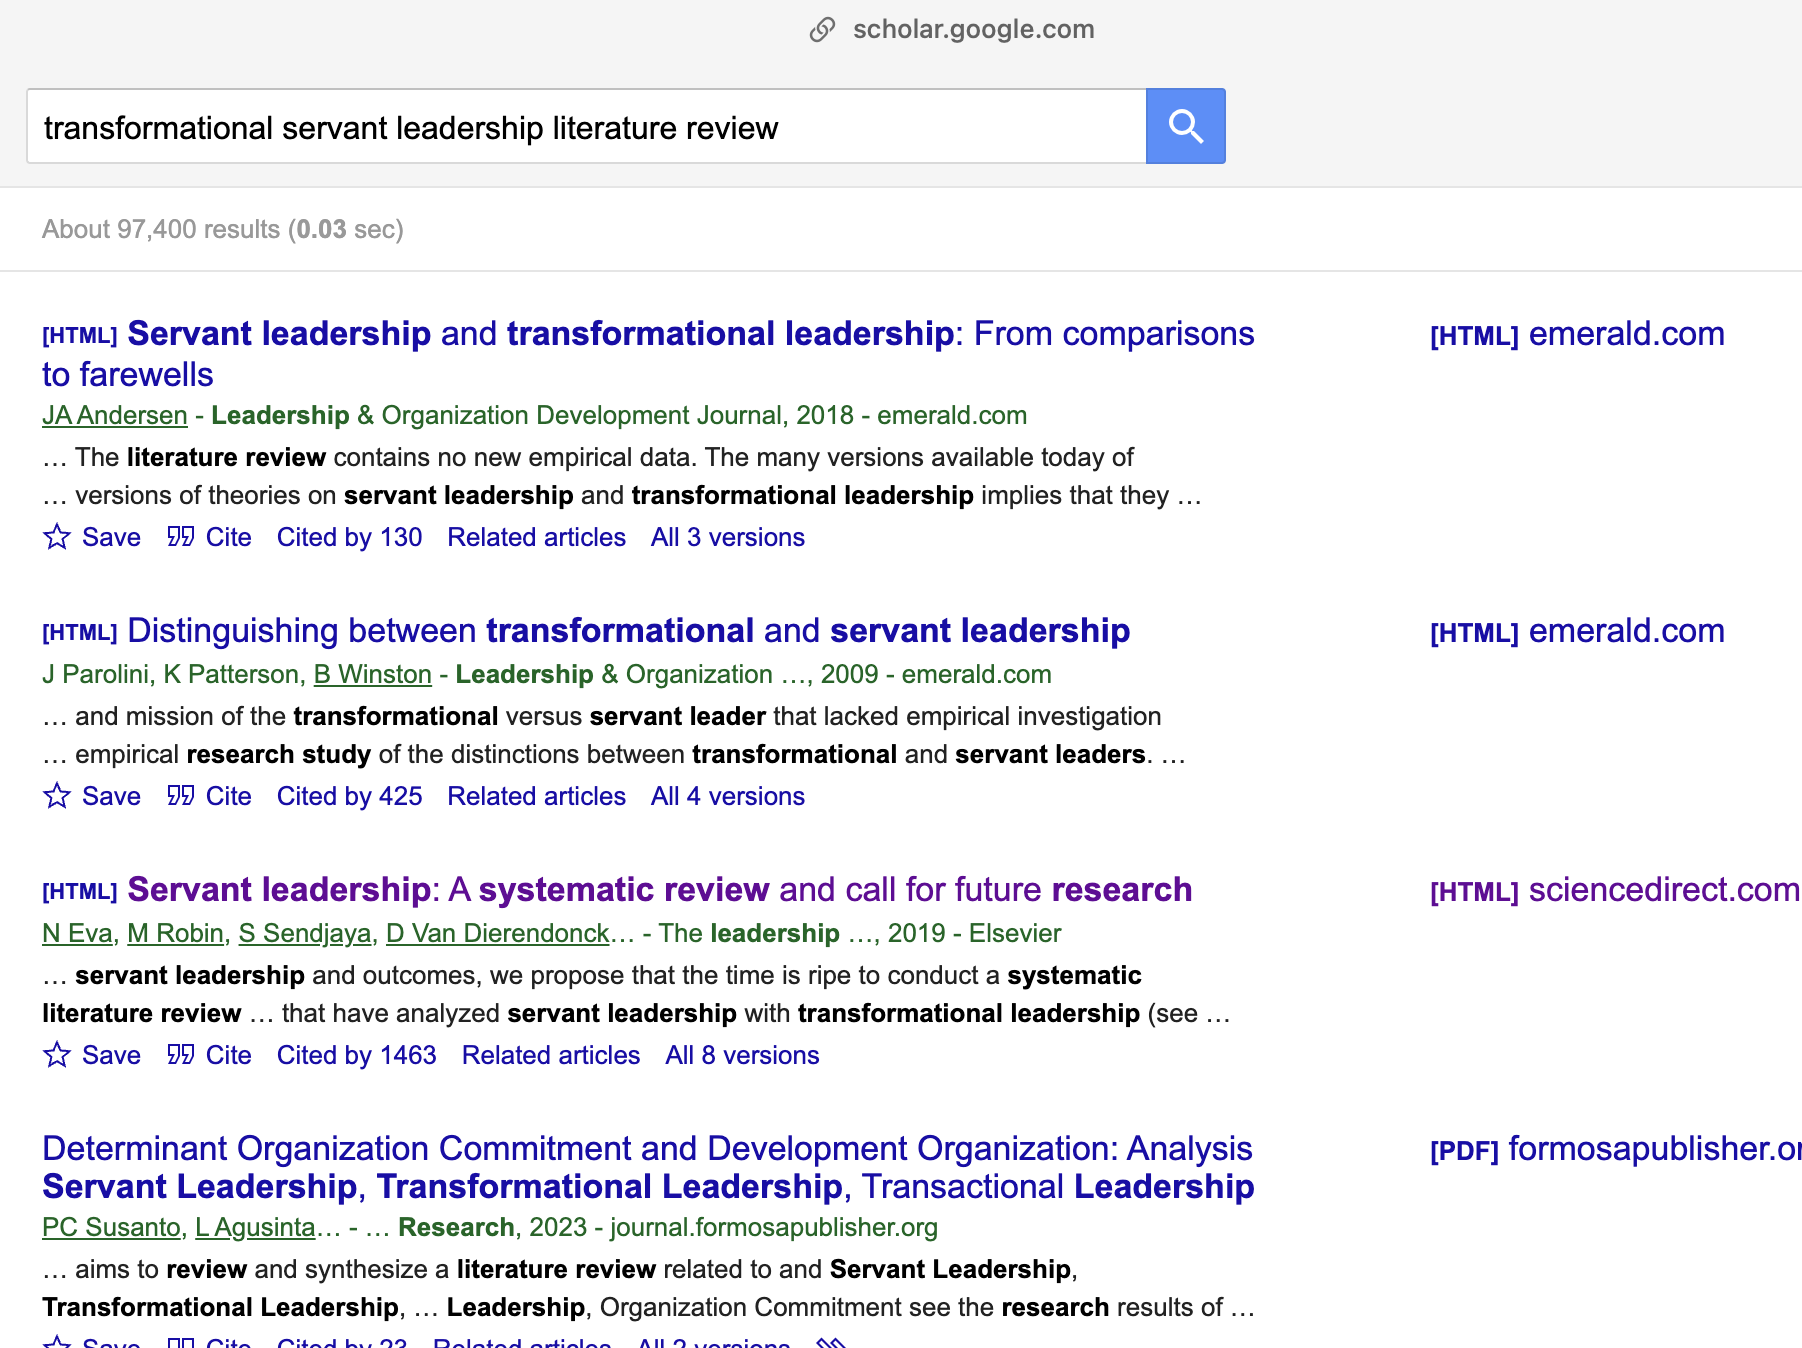
\includegraphics{assets/u2/google-search2.png}

}

\end{figure}%

The top result shows some promise though. Notice a few things about it:

\begin{itemize}
\tightlist
\item
  it has all your key words right in the title---that's good
\item
  it has over 2,700 citations (that's very good)
\item
  it was published in 2004 (that's not great \ldots{} it's old)
\end{itemize}

One of the easiest ways to find literature reviews in Google searches is
to include ``literature review'' in your search. When we do that, we get
a better list. This time, there are more results (97,000), but they are
better results. Notice the third item \ldots{}

\begin{figure}

\caption{\label{fig-googlexsearch2}Screenshot, Results Page of Google
Scholar search for ``Transformational Servant Leadership Literature
Review''}

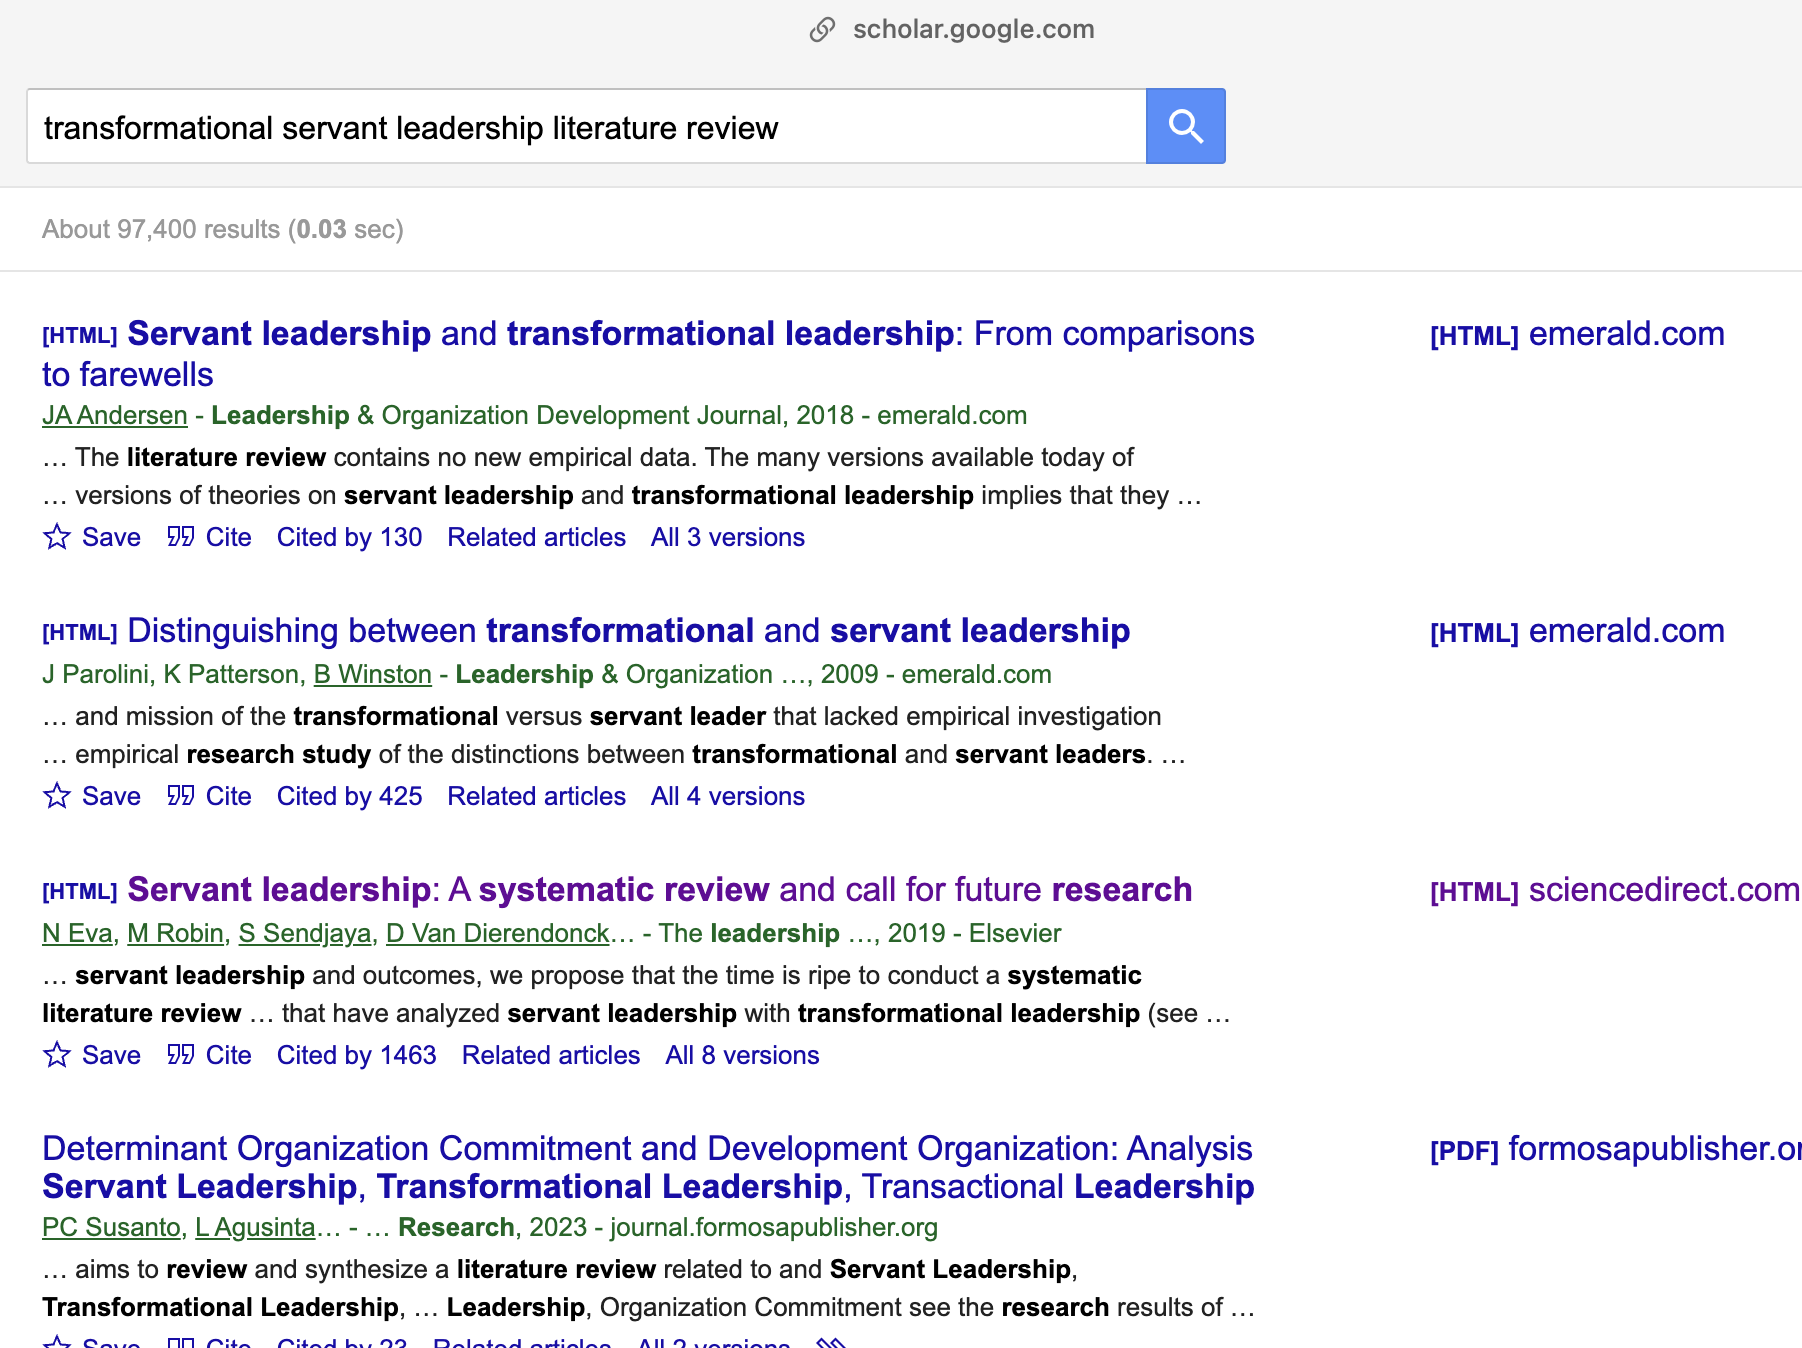
\includegraphics{assets/u2/google-search2.png}

\end{figure}%

\begin{itemize}
\tightlist
\item
  all your keywords
\item
  lots of citations
\item
  much more recent (2019)
\item
  AND it is a systematic review
\end{itemize}

This is the only article you need for now. Though search results are
always changing, we will use this example
\href{https://linkinghub.elsevier.com/retrieve/pii/S1048984317307774}{(Eva
et al., 2019)} in our upcoming activity. Click the link.

\begin{figure}

\caption{\label{fig-googlexsearch3}Screenshot of an Article Landing
Page}

\centering{

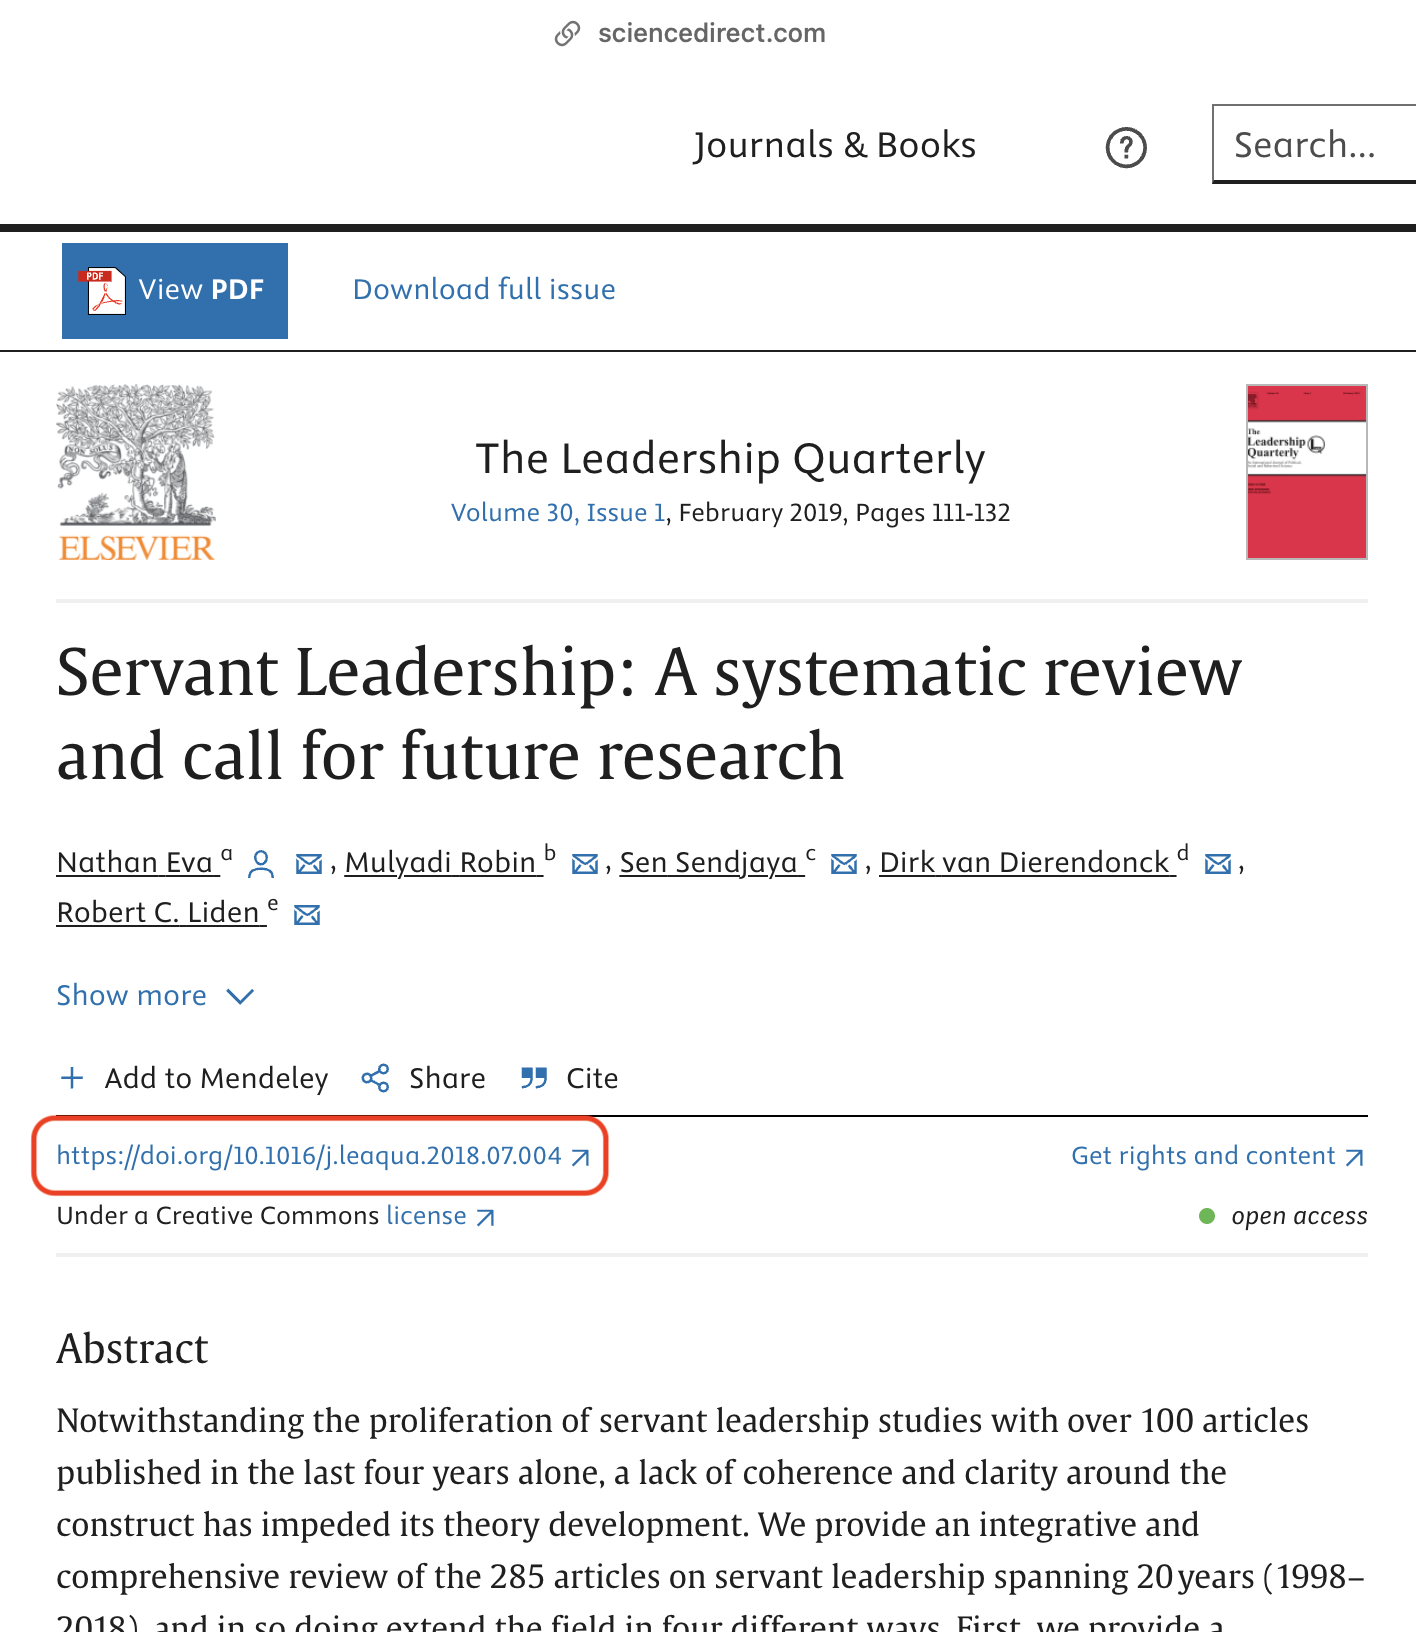
\includegraphics{assets/u2/google-search3.png}

}

\end{figure}%

In fact, you don't even need to read this article yet. All you need is
the DOI---the \emph{digital object identifier}. A DOI is a critical
piece of information about an article that provides a piece of evidence
that this is a legitimate article published in a legitimate journal. A
DOI will always start with 10. . Sometimes it is included as part of an
URL, as in this case, but you only need the code that follows `10.'. The
DOI for this article is \texttt{10.1016/j.leaqua.2018.07.004}

Copy the DOI. Sometimes you need to copy the whole URL, and that is ok.

\subsubsection{\texorpdfstring{Log in to
\href{https://www.litmaps.com/}{Litmaps.com} and paste the
DOI.}{Log in to Litmaps.com and paste the DOI.}}\label{log-in-to-litmaps.com-and-paste-the-doi.}

\begin{figure}

\caption{\label{fig-litmaps1}Screenshot of Litmaps Search Bar Populated
with a DOI}

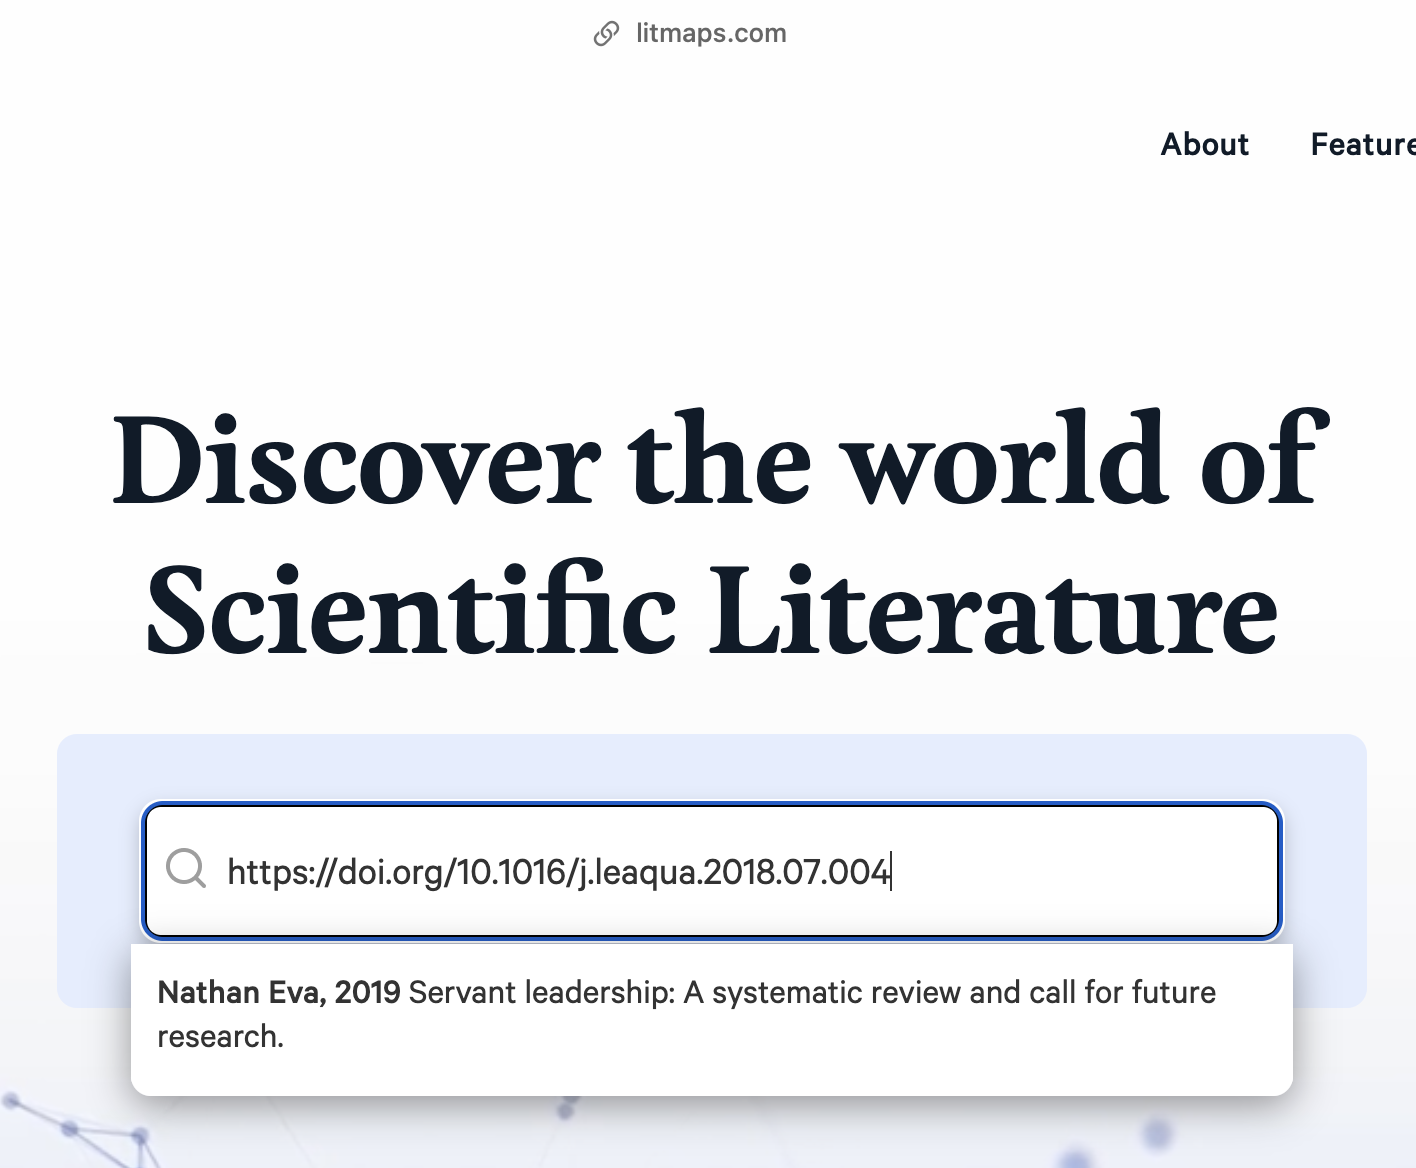
\includegraphics{assets/u2/litmaps1.png}

\end{figure}%

You will notice that LitMaps will be able to find the article and will
present it as an option for you to click. Go ahead \ldots{} click.

LitMaps will create what they call a Seed Map, which you can see in the
image below.

\begin{figure}

\caption{\label{fig-litmaps2}Screenshot of Litmaps Seed Map}

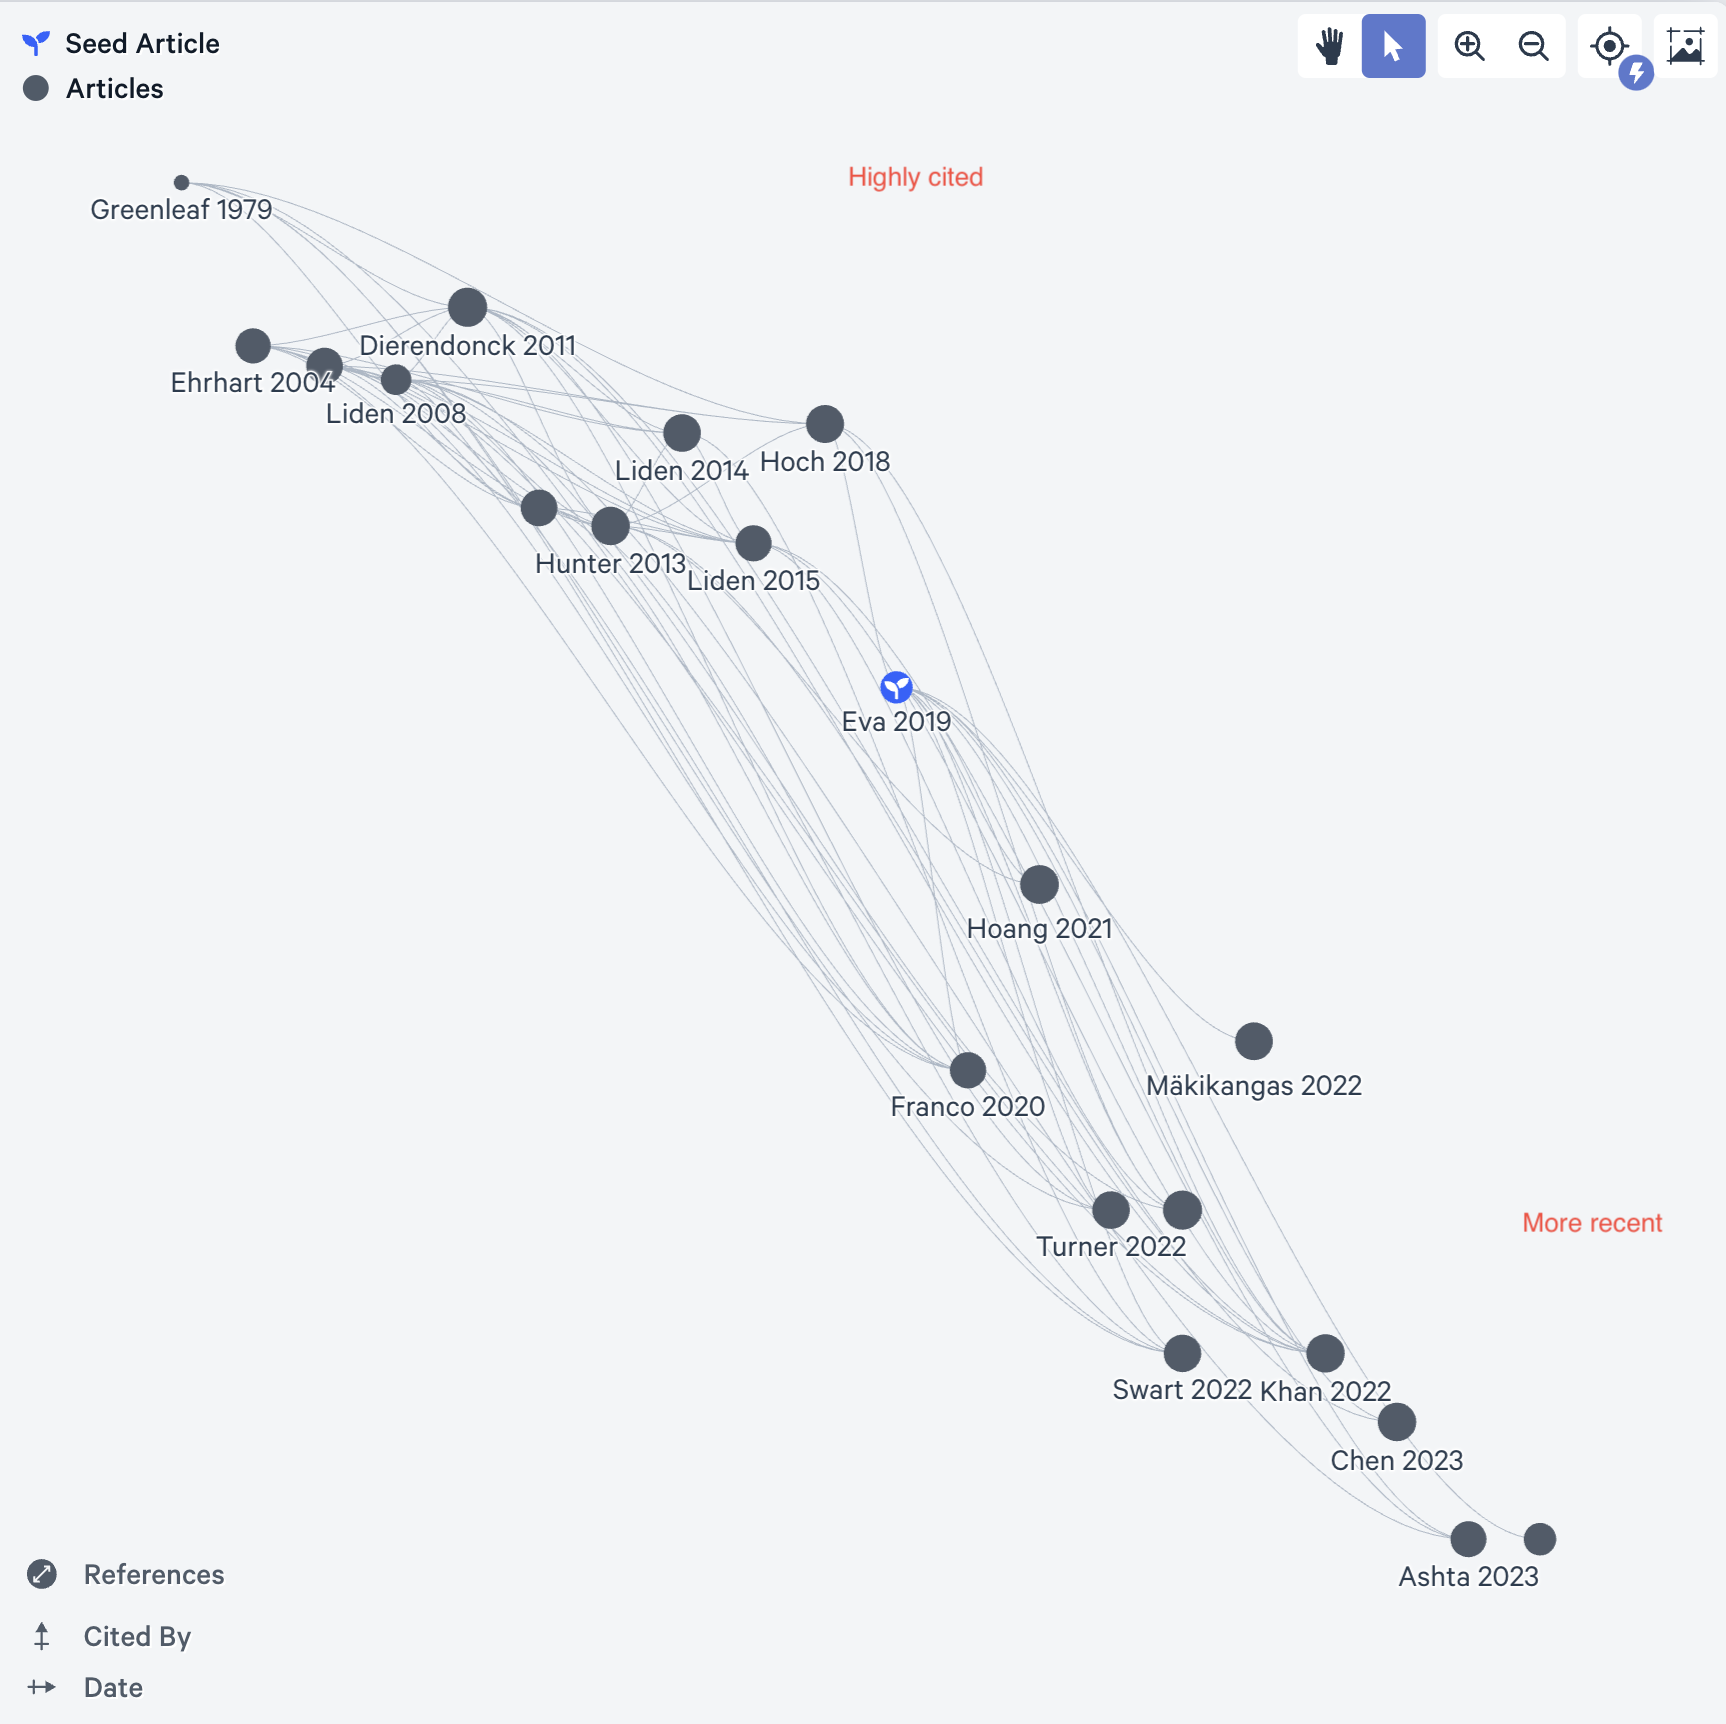
\includegraphics{assets/u2/litmaps2.png}

\end{figure}%

The seed map shows an AI-generated map of the 20 most relevant articles
related to the seed article. Each dot represents an article. The seed
article is shown as a blue dot with a little sprout in the middle. The
size of the dot is related to how many references are in the article
(smaller dot = fewer references). Dots near the top of the map have more
citations, and dots near the right side of the map are more recent. The
map will always look like a bit of a waterfall, as older articles tend
to have more citations. This map can be very helpful in finding very
impactful, recent articles as those articles will be in the top right
quadrant of the map.

When you are signed in to LitMaps you are able to create collections of
articles. To do this, click an article in the seed map, then read
through the abstract. This might tell you that the article is not
related to your search, but if it is, as in the image, then click ``Edit
Collections,''\,' then ``New Collection.'' Give the new collection a
name and click ``Done.''

\begin{figure}

\caption{\label{fig-litmaps3}Screenshot of Litmaps Seed Map with Edit
Collections Popup (Circled)}

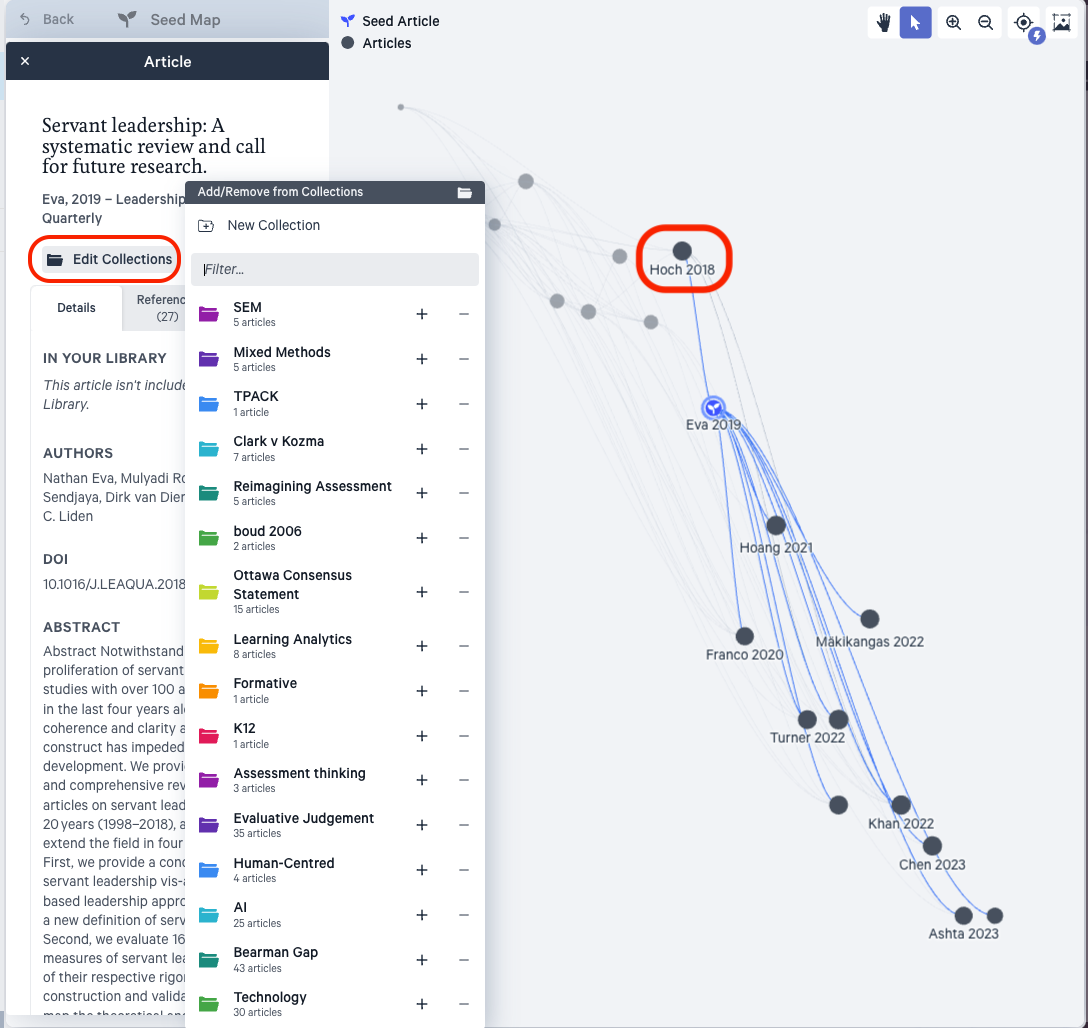
\includegraphics{assets/u2/litmaps3.png}

\end{figure}%

Next, add Hoch, 2018, to your new collection (it is closest to the upper
right quadrant), and finally add Greenleaf, 1979 (all the articles seem
to cite this article, so it is likely very important in the field,
sometimes called a seminal article).

Notice that the articles you added to your new collection are all
coloured the same as the collection.

\begin{figure}

\caption{\label{fig-litmaps4}Screenshot of Litmaps Seed Map Including
``Discover'' Option (Left)}

\centering{

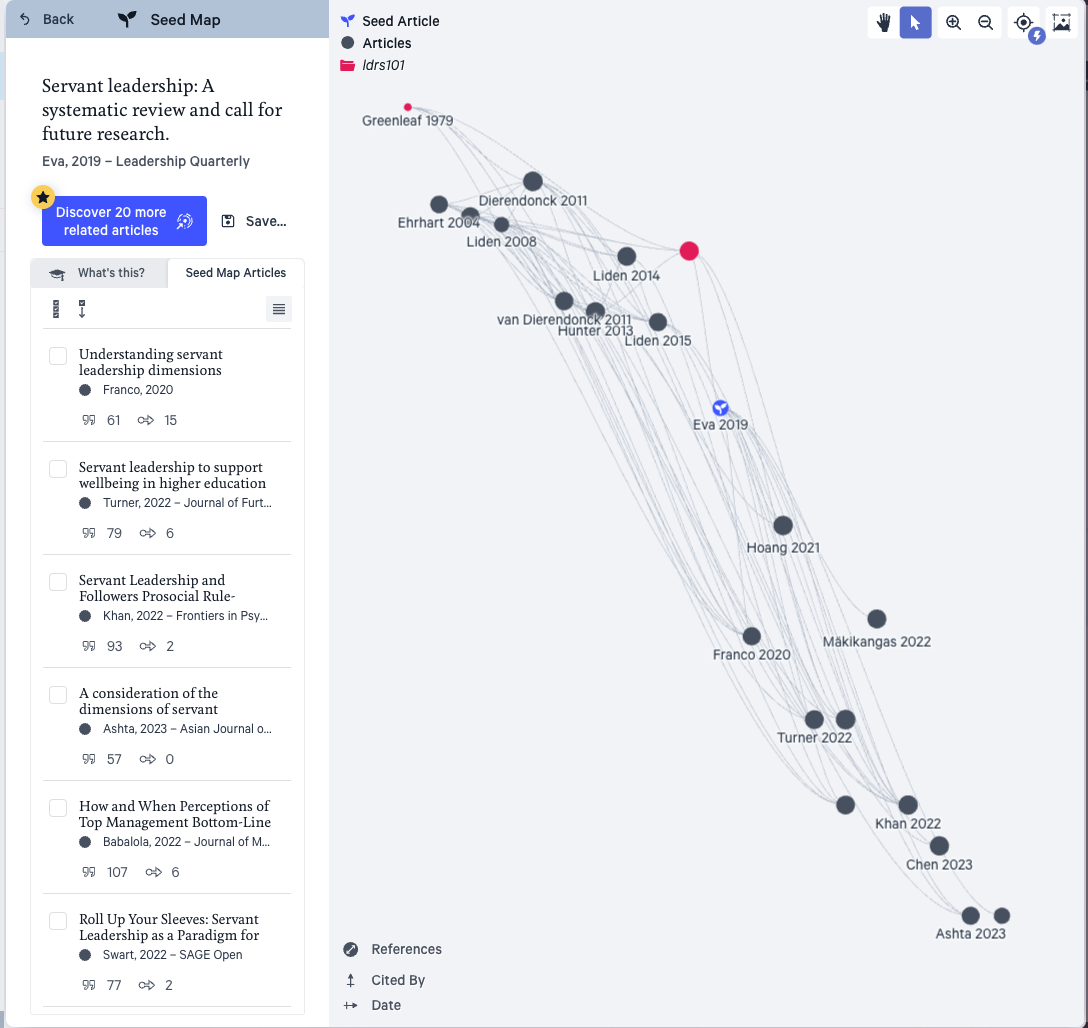
\includegraphics{assets/u2/litmaps4.png}

}

\end{figure}%

Next, click ``Discover'' in the lefthand menu bar, then click ``New
Search,'' then ``Add from your Library.''

\begin{figure}

\caption{\label{fig-litmaps5}Screenshot of Litmaps Seed Map Menu and
``Discover'' Link}

\centering{

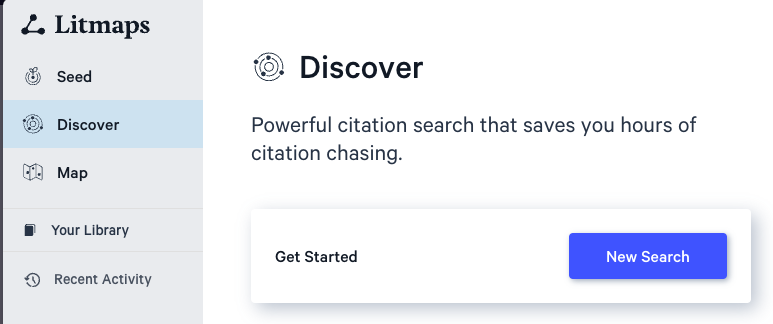
\includegraphics{assets/u2/litmaps5.png}

}

\end{figure}%

\begin{figure}

\caption{\label{fig-image9}Screenshot of Litmaps Seed Map ``Add from
Your Library'' Link (Circled)}

\centering{

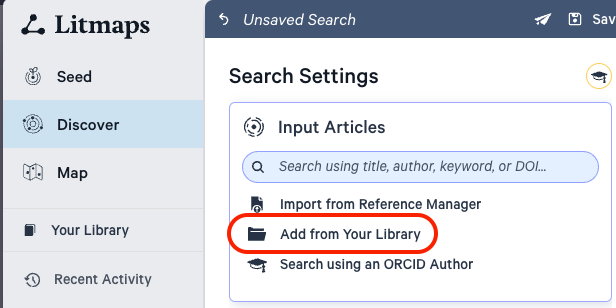
\includegraphics{assets/u2/image9.png}

}

\end{figure}%

Make sure you are in the correct collection (your collection should show
the Eva, Hoch, and Greenleaf articles you added), and click ``Add 3
Inputs.

\begin{figure}

\caption{\label{fig-litmaps7}Screenshot of Litmaps Seed Map Including
Collection Articles}

\centering{

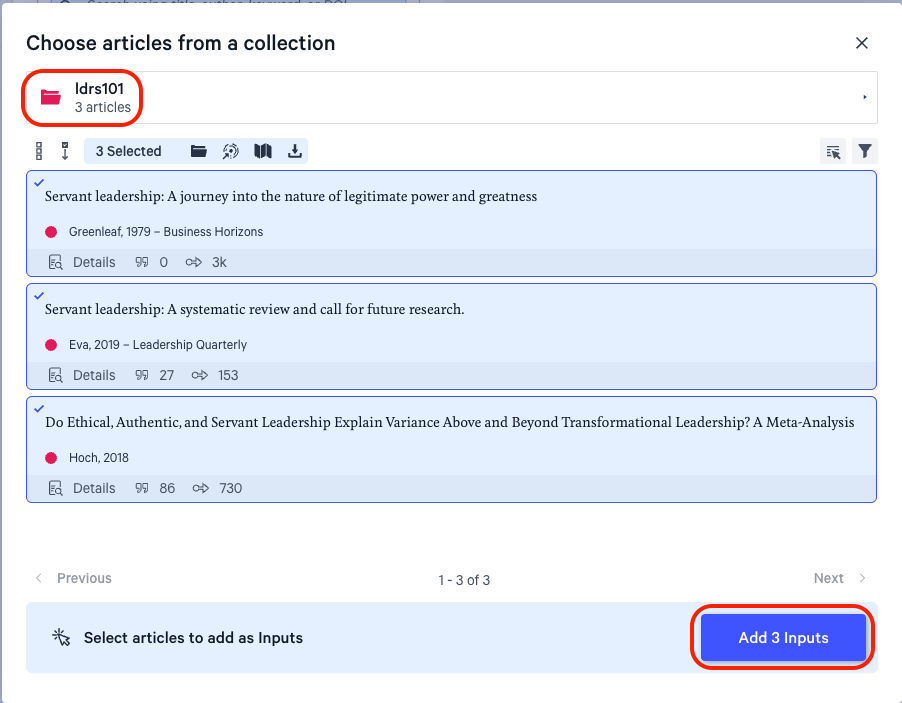
\includegraphics{assets/u2/litmaps7.png}

}

\end{figure}%

Then click ``Find Related Articles.''

\begin{figure}

\caption{\label{fig-litmaps8}Screenshot of Litmaps Seed Map Including
Selected Articles and ``Find Related Articles'' on Bottom Left Menu}

\centering{

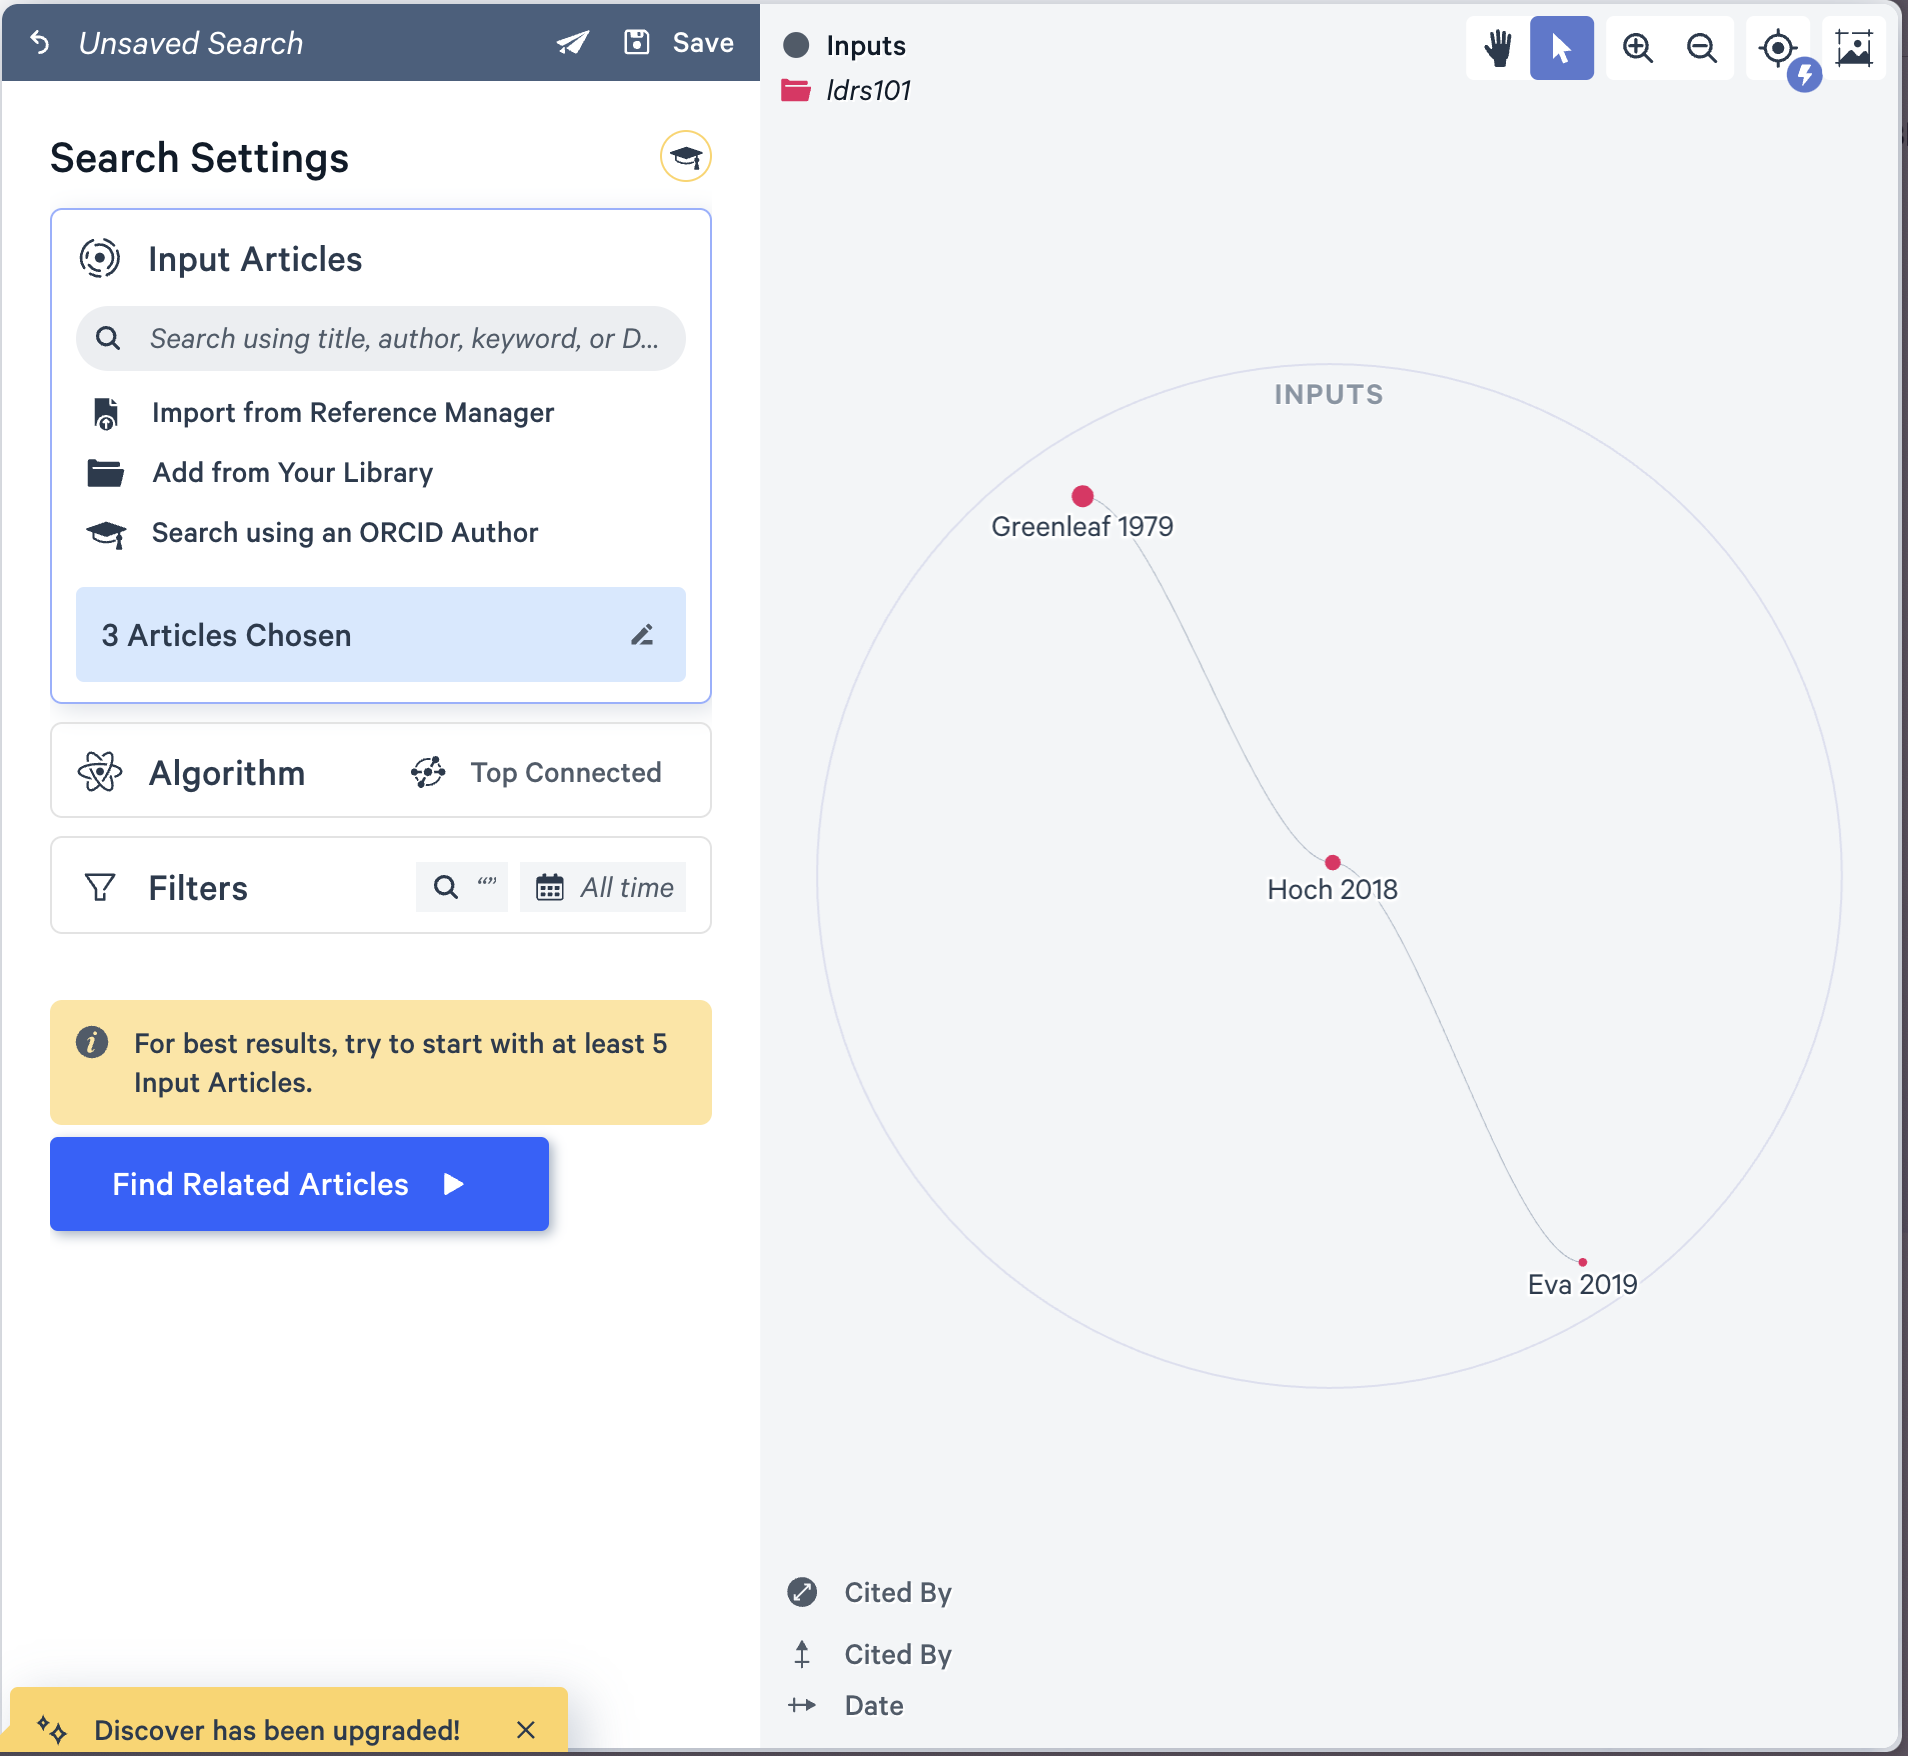
\includegraphics{assets/u2/litmaps8.png}

}

\end{figure}%

This will result in a new set of articles that are related to all three
of your initial input articles. As you add more inputs, you will get a
more refined result list until you have a nicely curated list of related
articles.

\begin{figure}

\caption{\label{fig-litmaps9}Screenshot of Litmaps Seed Map Showing
Articles Related to Those Previously Selected}

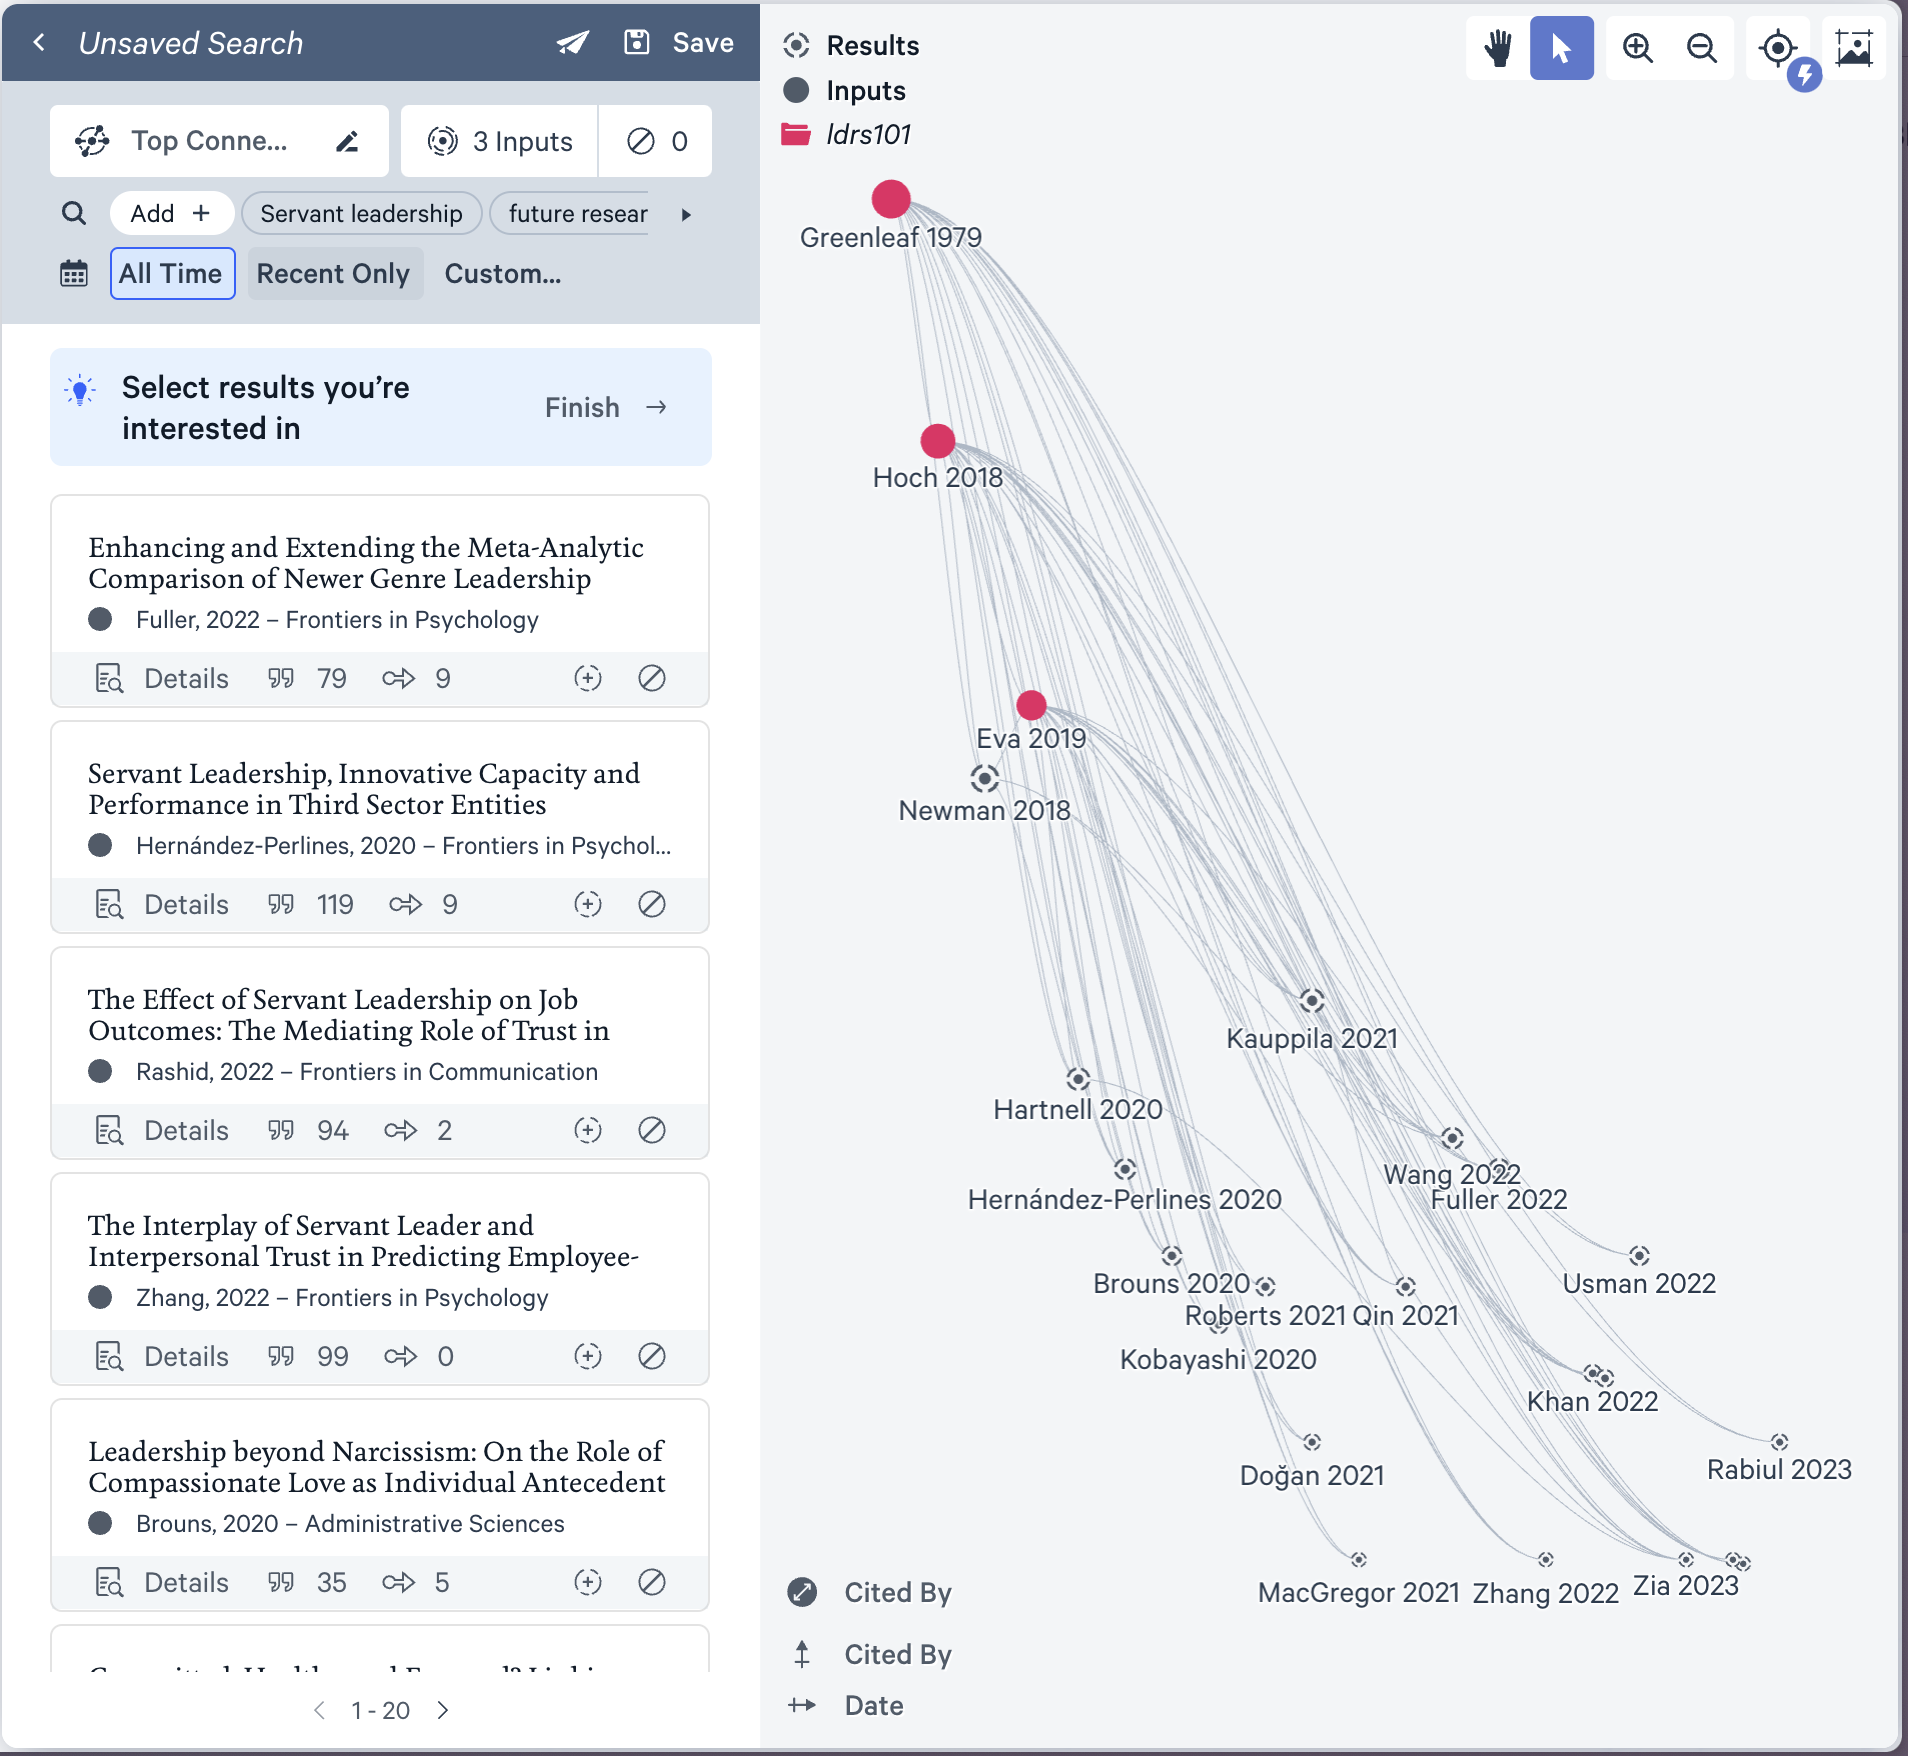
\includegraphics{assets/u2/litmaps9.png}

\end{figure}%

To add an input article, click it in the map or list and choose ``Add to
Search,'' then ``Expand Search'' to execute a new search with the new
articles you added.

\begin{figure}

\caption{\label{fig-litmaps10}Screenshot of Litmaps Seed Map Showing
Selected Article and ``Add to Search'' Button}

\centering{

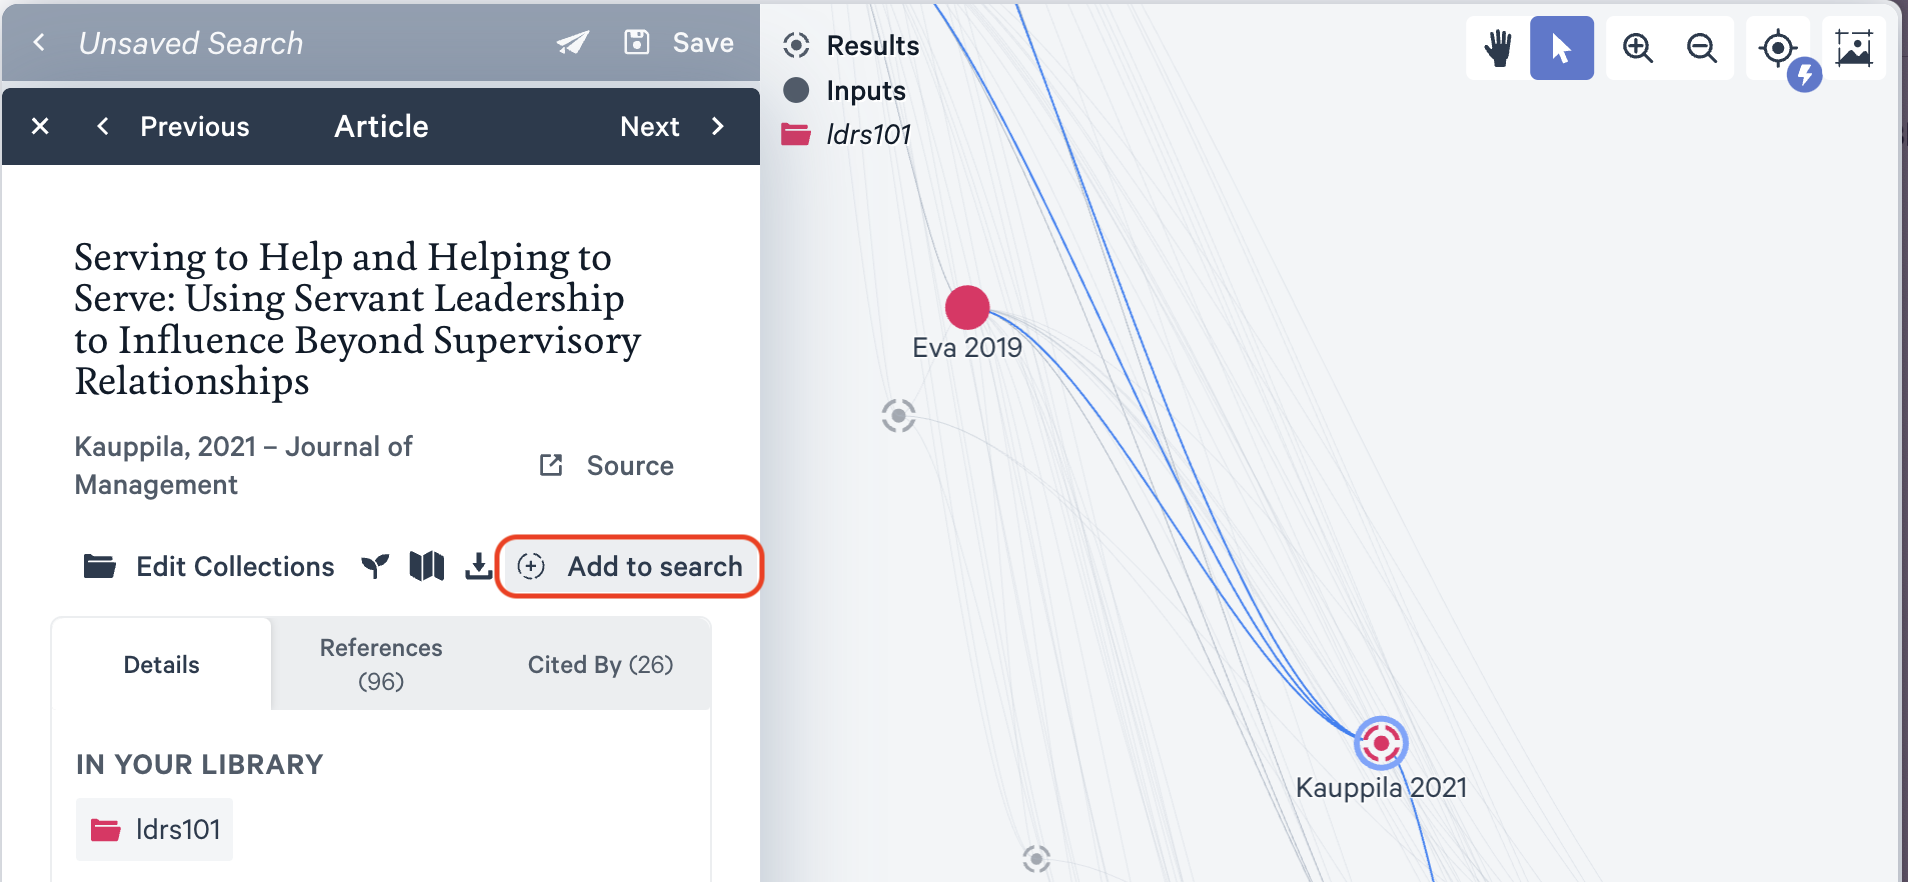
\includegraphics{assets/u2/litmaps10.png}

}

\end{figure}%

\begin{figure}

\caption{\label{fig-litmaps11}Screenshot of Litmaps Seed Map with
Additional Article Added}

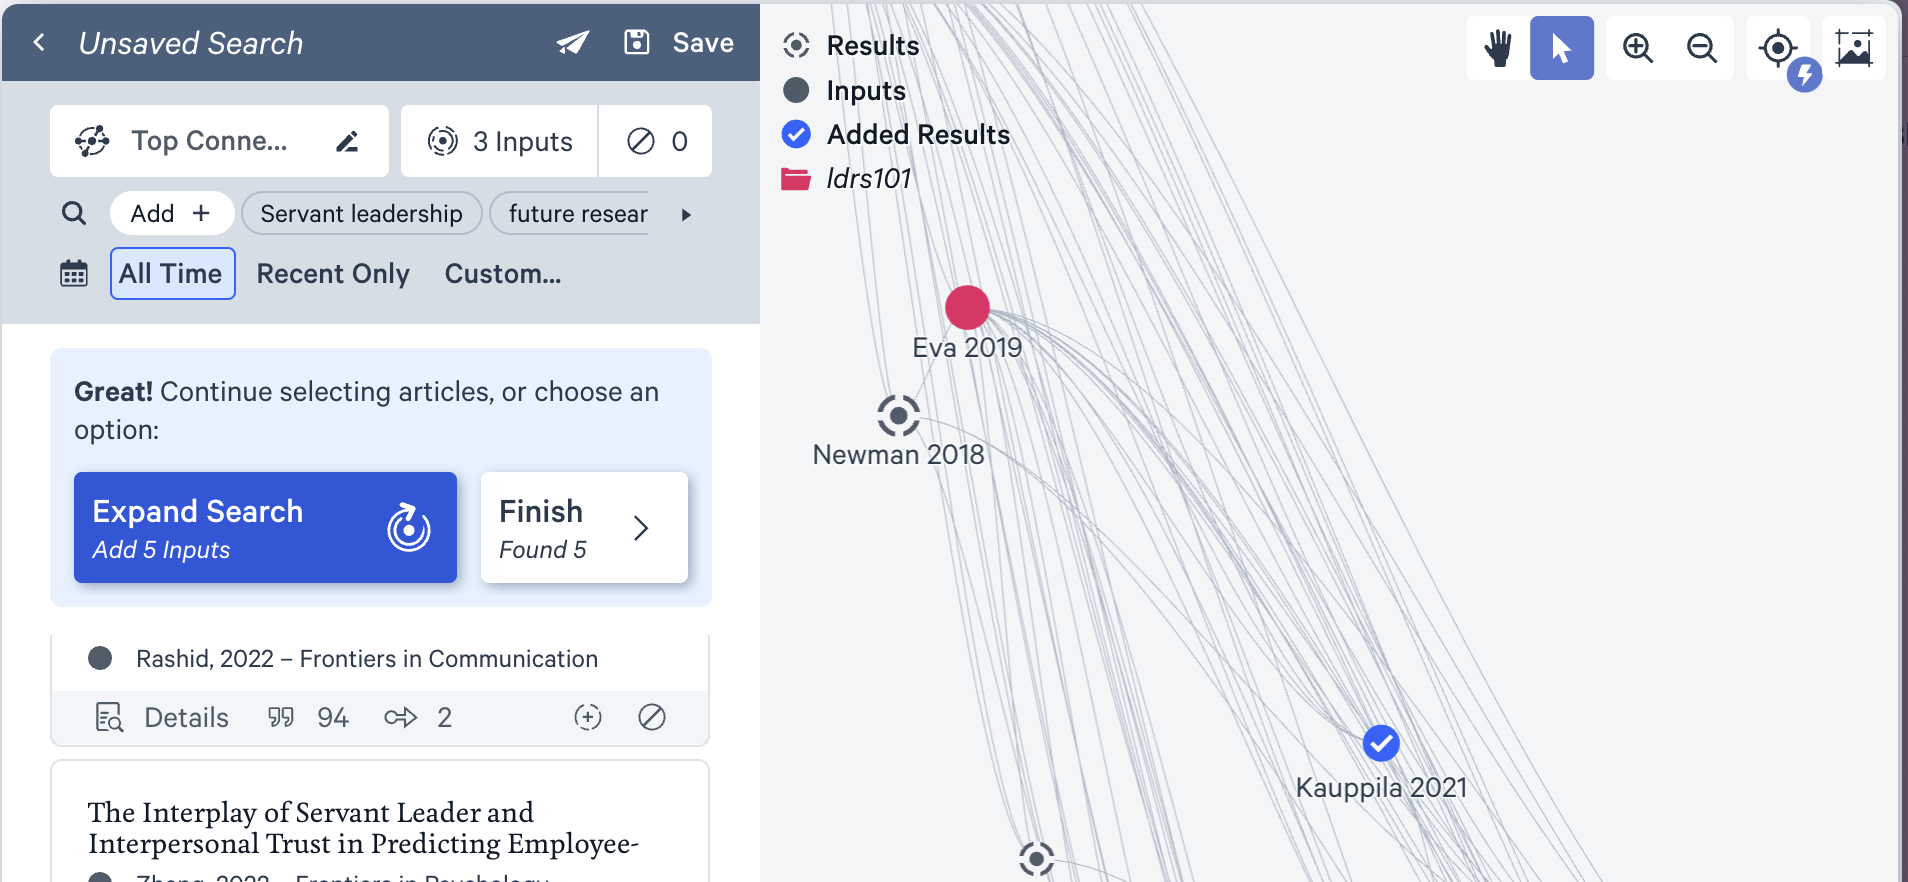
\includegraphics{assets/u2/litmaps11.png}

\end{figure}%

Notice that this search turned up another impactful article. Make sure
to add that to your list!

\begin{figure}

\caption{\label{fig-litmaps12}Screenshot of Litmaps Seed Map Showing
Additional Related Articles}

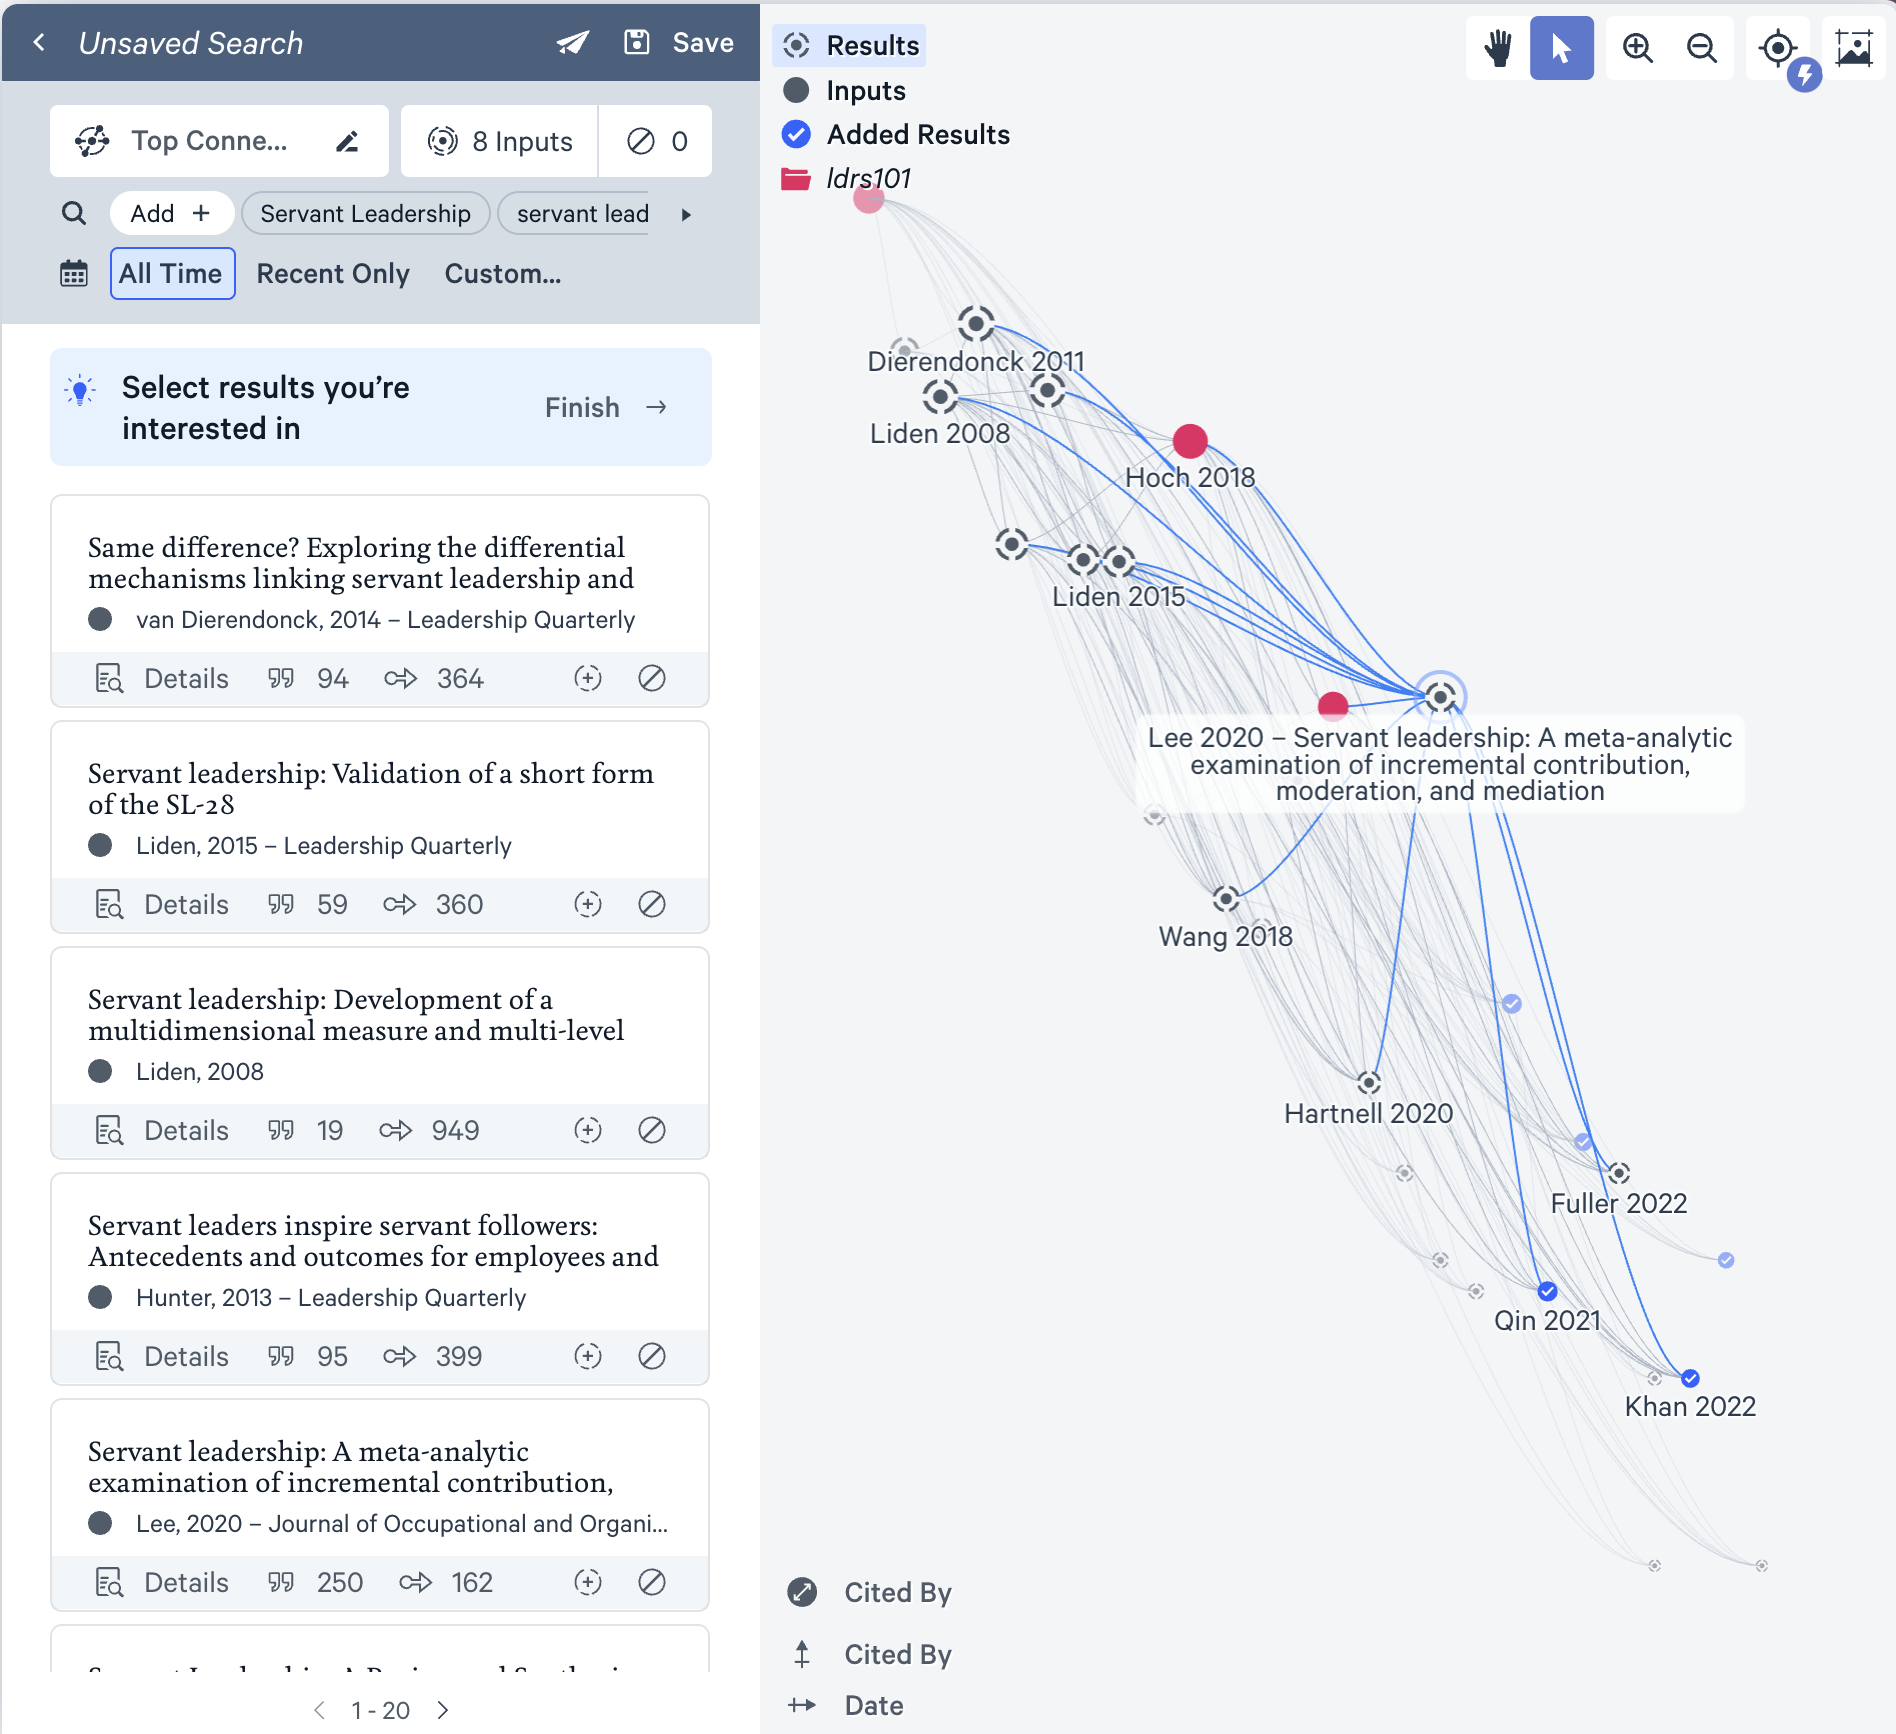
\includegraphics{assets/u2/litmaps12.png}

\end{figure}%

Next, click ``Your Library'' and choose the library you just created.
There should be eight or so references in the library. This is likely
enough to synthesize into a short paper, but some disciplines may
require more. Select all of the items in the library by clicking the
checkbox that initially says ``0 Selected,'' then click the ``Export''
(download) icon on the right side of the screen.

\begin{figure}

\caption{\label{fig-litmaps13}Screenshot of Litmaps Seed Map with
Library Entries Selected}

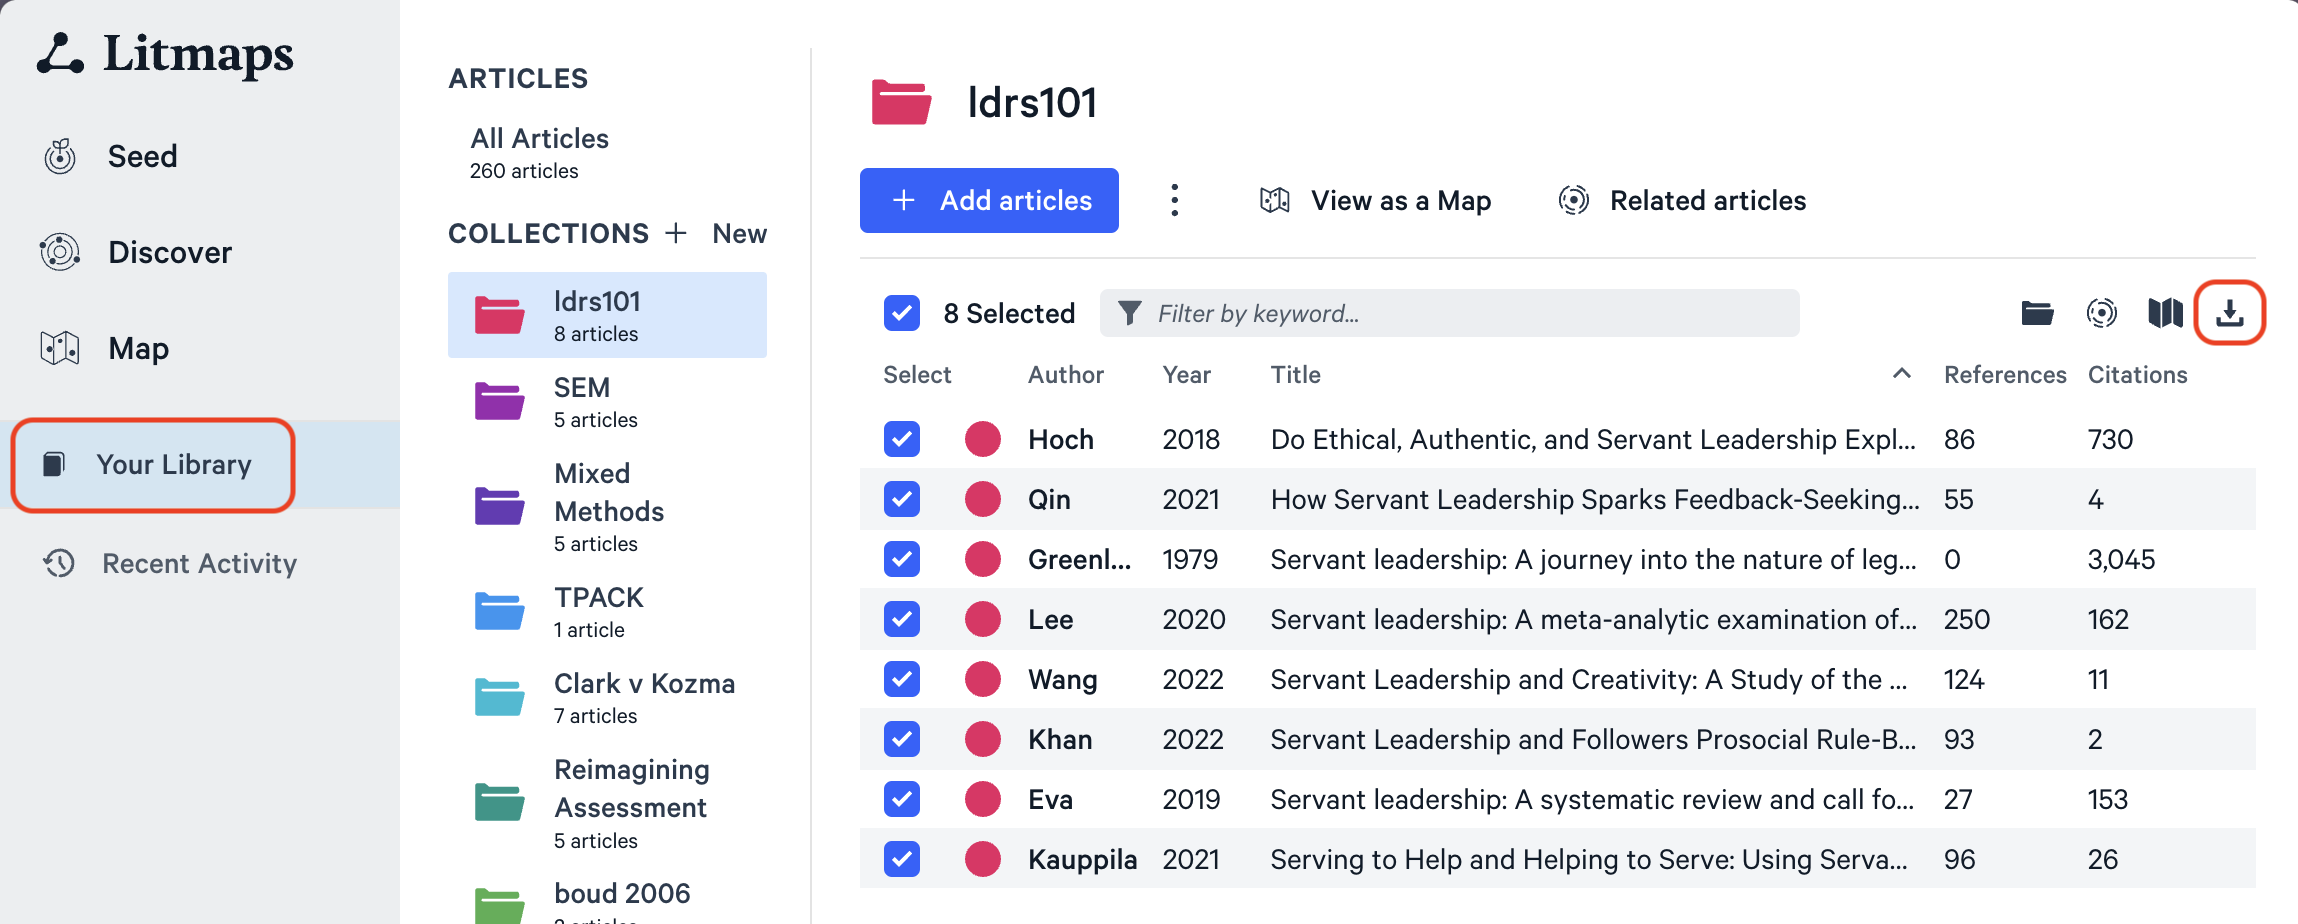
\includegraphics{assets/u2/litmaps13.png}

\end{figure}%

Choose ``RIS'' in the dropdown menu, then click ``Download.''

\begin{figure}

\caption{\label{fig-litmaps14}Screenshot of Litmaps Seed Map Menu for
Downloading Articles with RIS Format Selected}

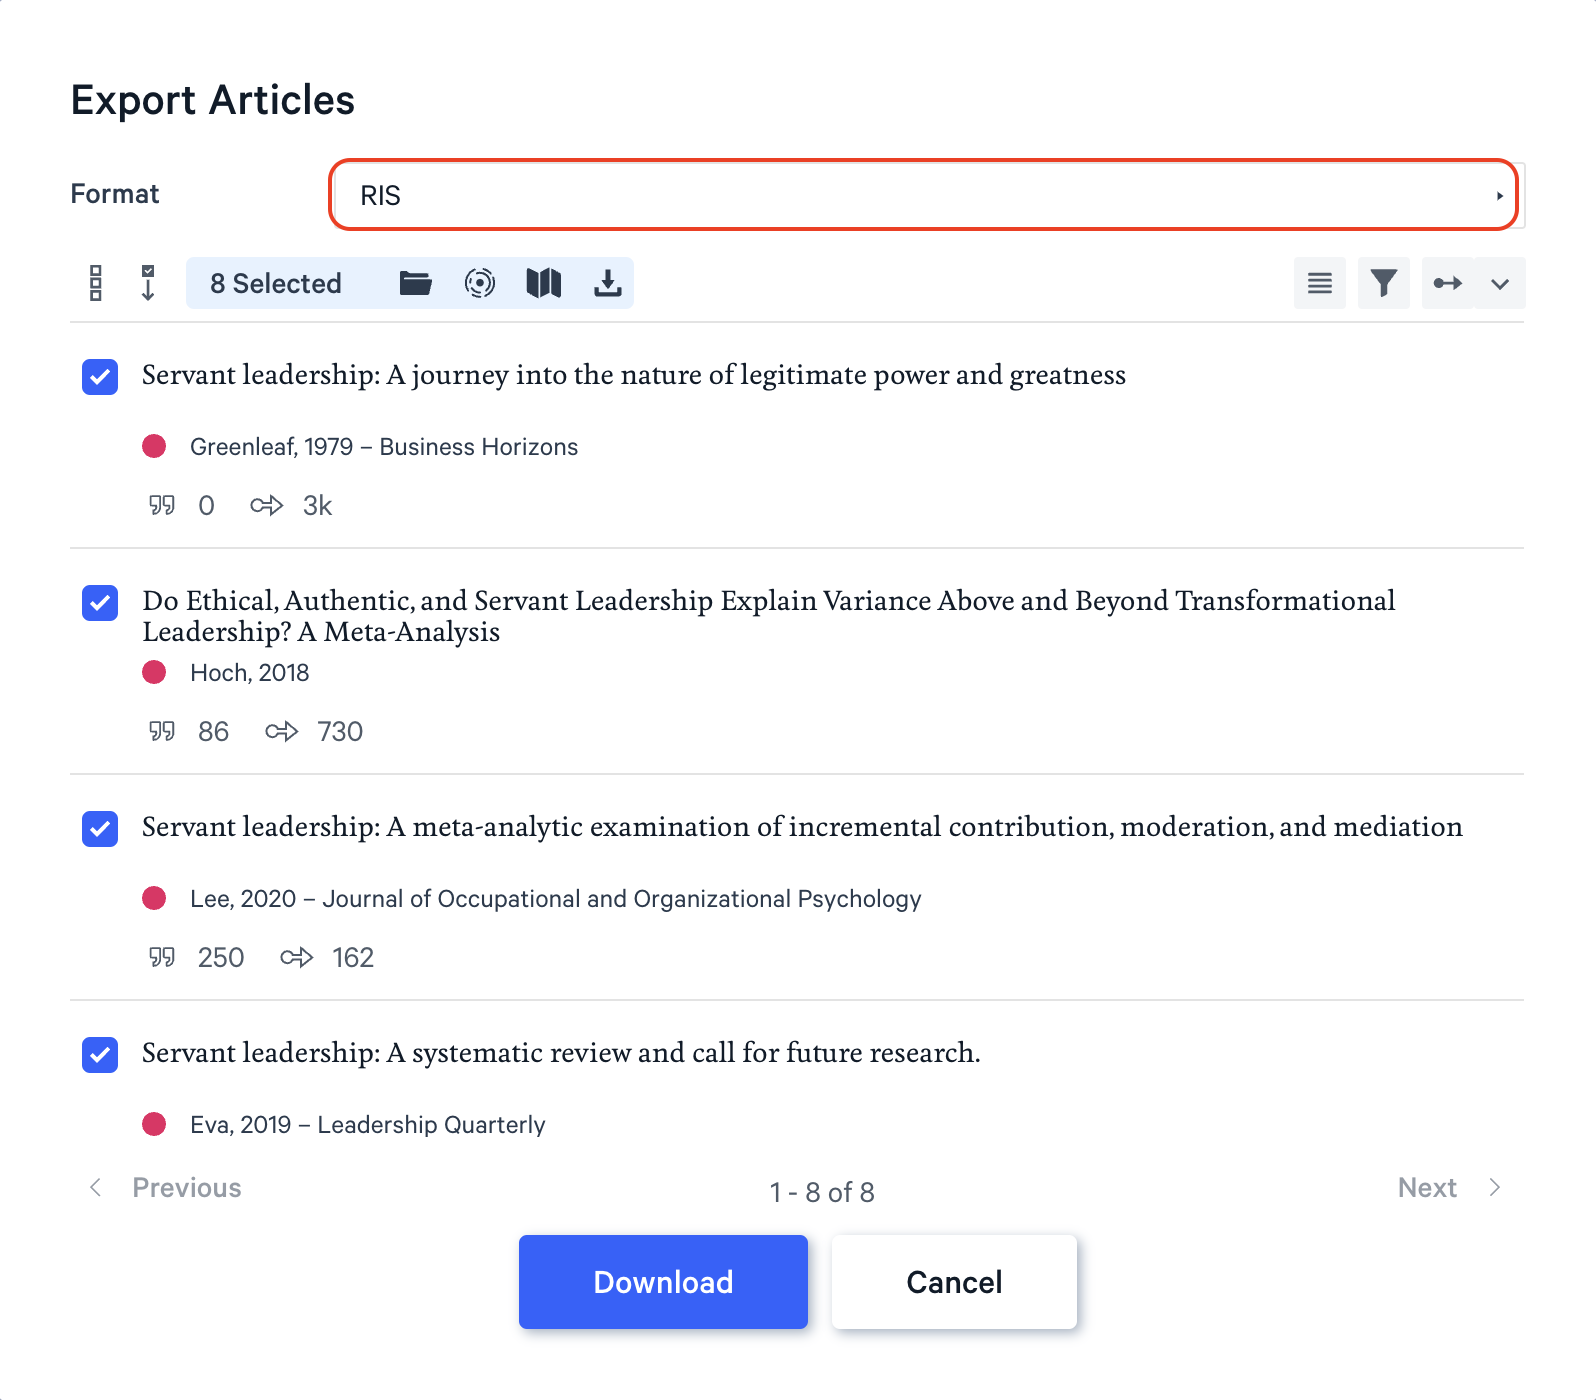
\includegraphics{assets/u2/litmaps14.png}

\end{figure}%

For more tutorials on using Litmaps, search online. For example, the
Litmaps YouTube channel has some helpful videos.

\begin{tcolorbox}[enhanced jigsaw, toprule=.15mm, colback=white, colframe=quarto-callout-note-color-frame, bottomtitle=1mm, leftrule=.75mm, coltitle=black, titlerule=0mm, rightrule=.15mm, colbacktitle=quarto-callout-note-color!10!white, left=2mm, title={Learning Activity}, opacitybacktitle=0.6, opacityback=0, breakable, toptitle=1mm, arc=.35mm, bottomrule=.15mm]

\begin{itemize}
\tightlist
\item
  \textbf{Research}: Choose a research topic that interests you. (Tip:
  Consider the course you are taking or will take in the future.) What
  key topics do you want to learn more about? Here are some other links
  that may help you decide:

  \begin{itemize}
  \tightlist
  \item
    \emph{Choosing a Topic: Purdue OWL}
    \href{https://owl.purdue.edu/owl/general_writing/common_writing_assignments/research_papers/choosing_a_topic.html}{(n.d.-b)}
  \item
    \emph{Building Your Research Skills}
    \href{https://libguides.twu.ca/ResearchSkills/Home}{(2024)}
  \item
    Conduct a general internet search for ``Topical issues in Business''
    or ``Topical issues in Higher Education'' and scan whether any of
    these issues are of personal interest.
  \end{itemize}
\item
  \textbf{Write}: State your topic in the form of a question. For
  example:

  \begin{itemize}
  \tightlist
  \item
    How will robotics impact the future of work?
  \item
    What can businesses do to run successful loyalty programs?
  \item
    How can technology prepare learners for a future that is
    increasingly defined within the context of globalization and
    technology?
  \item
    How will mobile technology impact diagnosis and health care?
  \end{itemize}
\item
  \textbf{Review} your draft research question taking into account:

  \begin{itemize}
  \tightlist
  \item
    \emph{Personal interest}: Does the research question interest you?
  \item
    \emph{Suitability for academic investigation}: Some questions are
    not possible to answer through academic enquiry, for example, ``How
    beautiful is the colour orange?'' Identify a few keywords related to
    your proposed research question and conduct a general search to
    determine if there are published and accessible research outputs
    related to your question.
  \item
    \emph{Attainability}: Make sure that your question can be answered
    in the amount of time you have. For example, ``How do we solve
    global disease?'' is too broad, whereas, ``What is my neighbour's
    favourite colour?'' is too narrow. You will be looking to target
    between 8 to 15 scholarly references to prepare an annotated
    bibliography, including books, journal articles, and reputable
    website references . From those you will choose three for your
    annotated bibliography activity you will complete at the end of the
    unit.
  \item
    Use Litmaps to explore the literature on the topic of your choice.
  \end{itemize}
\item
  \textbf{Reflect}: Take a screenshot of your Litmaps map and paste it
  to a journal entry in Obsidian. Reflect on your use of this tool. What
  was difficult to learn? How might you use this tool in your future
  studies?
\end{itemize}

\subsection{Activity: the TWU Library}\label{activity-the-twu-library}

\begin{tcolorbox}[enhanced jigsaw, toprule=.15mm, colback=white, colframe=quarto-callout-note-color-frame, bottomtitle=1mm, leftrule=.75mm, coltitle=black, titlerule=0mm, rightrule=.15mm, colbacktitle=quarto-callout-note-color!10!white, left=2mm, title={Learning Activity}, opacitybacktitle=0.6, opacityback=0, breakable, toptitle=1mm, arc=.35mm, bottomrule=.15mm]

Some of your best advocates on campus or online are the librarians who
work at the Norma Marion Alloway Library in Langley. They are extremely
knowledgeable about finding things that are hard to find, so it is
ALWAYS a good idea to talk to a librarian about what you are trying to
do. They are literally paid to help you succeed! One of the ways they
like to help is by creating what is known as a ``LibGuide,'' and we
encourage you to access the LibGuides by selecting Research Guides on
the \href{https://www.twu.ca/academics/library\#}{library website}.

Take some time to browse the
\href{https://www.twu.ca/academics/library}{TWU Library}. See if you can
find the answer to the following questions:

\begin{itemize}
\tightlist
\item
  Is it possible to borrow or download an ebook?
\item
  I'm a distance student. Can I request to have books or articles sent
  from the TWU Library to my location?
\item
  Do you have books in languages other than English?
\item
  Do you have ebooks?
\item
  Can I email a Trinity Western librarian any time with my research
  questions?
\item
  What is AskAway?
\item
  What do I do if I have trouble logging in to library databases from
  off campus?
\end{itemize}

\end{tcolorbox}

\subsection{Activity: Advanced Search}\label{activity-advanced-search}

\begin{tcolorbox}[enhanced jigsaw, toprule=.15mm, colback=white, colframe=quarto-callout-note-color-frame, bottomtitle=1mm, leftrule=.75mm, coltitle=black, titlerule=0mm, rightrule=.15mm, colbacktitle=quarto-callout-note-color!10!white, left=2mm, title={Learning Activity}, opacitybacktitle=0.6, opacityback=0, breakable, toptitle=1mm, arc=.35mm, bottomrule=.15mm]

Improving search skills will save you time and result in more productive
searches. Although we focus on LitMaps and the TWU Library in this
course, another tool we want to share is the Google search engine. It
provides a number of features to improve your searches in finding
academic resources. In this activity, you will select two open resources
using the Google advanced search operators in support of your research
topic.

\begin{itemize}
\tightlist
\item
  \textbf{Read}: the
  \href{https://www.webfx.com/blog/seo/google-advanced-search-operators-cheat-sheet/}{\emph{Google
  Search Cheatsheet}} for a more comprehensive list.Also see the
  \href{https://quickref.me/google-search.html}{\emph{Google Advanced
  Search Operators Cheat Sheet}} (n.d.) and try a few searches using the
  operators.
\end{itemize}

\begin{itemize}
\tightlist
\item
  \textbf{Search}: Use the Google search operators (enter these directly
  into the search text area) to:

  \begin{itemize}
  \tightlist
  \item
    identify at least 10 PDF documents which have open educational
    resources in their title (are they all accessible for download?)
  \item
    find a PDF version of the editorial entitled \emph{Scholarship and
    Literacies in a Digital Age} (who are the authors?)
  \item
    Find the article with the following citation in text: the term
    digital literacies is contested with differing uses of the term
    revealing competing and even contradictory theoretical perspectives
    (who is the author?)
  \end{itemize}
\end{itemize}

Visit the \href{https://www.google.com/advanced_search}{Google Advanced
Search} web interface:

\begin{itemize}
\tightlist
\item
  conduct a search for digital literacies and scan the results
\item
  go back to the Google Advanced Search web interface and remove words
  from the search, for example ``skills'' or ``school'' and compare the
  results
\item
  click tools and find results for the date range 1 May 2020 to 1 May
  2023
\item
  click images and find versions which are licensed for reuse with
  modification (useful when sourcing images for your course blog with
  the necessary legal permissions for reuse)
\end{itemize}

\textbf{Other Search Engines}

Google Scholar is a good search engine to find scholarly publications.
The downside is that Google Scholar does not distinguish between closed
and open resources. However, search results which show a PDF next to the
listing will probably provide access to a full text version. Unpaywall
is a free and legal way to identify authored--uploaded PDFs. There are
extensions for the Chrome and Firefox open source browsers. Read the
frequently asked questions for more information.

\end{tcolorbox}

\subsection{Activity: Database Search}\label{activity-database-search}

\begin{tcolorbox}[enhanced jigsaw, toprule=.15mm, colback=white, colframe=quarto-callout-note-color-frame, bottomtitle=1mm, leftrule=.75mm, coltitle=black, titlerule=0mm, rightrule=.15mm, colbacktitle=quarto-callout-note-color!10!white, left=2mm, title={Learning Activity}, opacitybacktitle=0.6, opacityback=0, breakable, toptitle=1mm, arc=.35mm, bottomrule=.15mm]

This activity focuses on searching database repositories. Most databases
provide advanced search features; however there are differences in how
each database site implements search functionality.

\begin{itemize}
\tightlist
\item
  \textbf{View} the following resources on searching using databases.

  \begin{itemize}
  \tightlist
  \item
    \href{https://www.berkeleycitycollege.edu/library/2011/04/04/databasesearchtips/}{\emph{Top
    Ten Database Search Tips} (2011)}
  \item
    \emph{Searching in Databases}
    \href{https://web.library.uq.edu.au/research-tools-techniques/search-techniques/where-and-how-search/searching-databases}{(2012)}
  \item
    \href{https://doaj.org/}{Directory of Open Access Journals (DOAJ)}
    -- see also FAQs
  \end{itemize}
\item
  \textbf{Watch} the following video
  \href{https://www.youtube-nocookie.com/embed/ndvLm9MIfKA}{Directory of
  Open Access Journals (DOAJ)} on using the (2016)
\end{itemize}

\url{https://www.youtube-nocookie.com/embed/ndvLm9MIfKA}

\begin{itemize}
\tightlist
\item
  Using your keywords and synonyms generated for your research question,
  search for journal articles using the DOAJ search engine and BASE
  Advanced Search.
\item
  As appropriate, adapt your search by narrowing or expanding---remember
  to be flexible; if one term doesn't work, try a different one.
\item
  Select a minimum of two resources, more if you like to save time later
  in the course.
\item
  Based on the resources you find, think about whether you need to
  modify your research question.
\end{itemize}

How was your progress with this activity? Feel free to share your
thoughts in Obsidian. For example:

\begin{itemize}
\tightlist
\item
  finding resources for my topic was \ldots{}
\item
  I found \ldots{} helpful.
\item
  database search tip: when \ldots{}
\end{itemize}

\end{tcolorbox}

\section{Evaluating Resources}\label{evaluating-resources}

A key part of finding and selecting resources is evaluating the
resource. There is a great deal of information available on the
internet. Some of it is very credible and useful. However, there is a
lot of misinformation and poorly researched information online too. As
you become more skilled at academic online searching and locating
materials you will become quicker at determining what information is
useful and credible.

So how do you evaluate sources to ensure those you are using are
credible? The following technique, called the CRAAP test, will help you
evaluate the sources you find.

\textbf{C} - Currency \textbf{R} - Relevance \textbf{A} - Authority
\textbf{A} - Accuracy \textbf{P} -- Purpose

\subsection{Activity: Using the Craap
Test}\label{activity-using-the-craap-test}

::: \{.learning-activity\}{]}

\begin{itemize}
\tightlist
\item
  \href{https://www.youtube.com/watch?v=_M1-aMCJHFg}{\textbf{Watch}:
  \emph{How Library Stuff Works: How to Evaluate Resources (the CRAAP
  Test)}} (2015). This illustrates a set of steps you could take to
  evaluate sources.
\end{itemize}

\url{https://www.youtube-nocookie.com/embed/_M1-aMCJHFg}

\begin{itemize}
\tightlist
\item
  \textbf{Questions To Consider:} After watching this video consider
  these questions:

  \begin{itemize}
  \tightlist
  \item
    Which part of the CRAAP test did you find most useful in evaluating
    sources?
  \item
    What following steps can you take when you evaluate any sources you
    find?
  \end{itemize}
\end{itemize}

\end{tcolorbox}

\subsubsection*{Reliability of
Wikipedia}\label{reliability-of-wikipedia}
\addcontentsline{toc}{subsubsection}{Reliability of Wikipedia}

Wikipedia is the free online encyclopedia created through the
collaborative effort of contributors from around the globe. Wikipedia is
one of the most popular websites in the world. When conducting general
internet searches Wikipedia articles will frequently be listed in the
top results.

Anyone registered on the Wikipedia site can create a new article page.
Anyone can edit a Wikipedia article, and registration is not required to
edit existing articles.

There have been a number of studies examining the accuracy of Wikipedia
articles. Notwithstanding the outcomes of these studies, many
educational institutions do not accept the use of Wikipedia as a
credible source for academic writing and research. In this section we
invite learners to evaluate whether Wikipedia is a trustworthy resource,
and to form a justified opinion on its use as a reliable resource for
academic writing.

\subsection{Activity: Wikipedia: Why or Why
Not?}\label{activity-wikipedia-why-or-why-not}

Consider the following statement: Wikipedia is a reliable source for
academic study.

Do you agree? Have you cited Wikipedia in any academic work? Why or why
not?

\begin{itemize}
\tightlist
\item
  \textbf{Read} the following:

  \begin{itemize}
  \tightlist
  \item
    \href{https://edtechmagazine.com/higher/article/2017/12/wikipedia-trustworthy-academic-resource-scientists-think-so}{Is
    Wikipedia a Trustworthy Academic Resource? Scientists Think So}
    published by EdTech Magazine.
  \item
    \href{https://en.wikipedia.org/wiki/Reliability_of_Wikipedia}{Reliability
    of Wikipedia} article on Wikipedia.
  \item
    \href{https://www.theguardian.com/education/2013/may/13/should-university-students-use-wikipedia}{\emph{Should
    University Students use Wikipedia?}}(2013)
  \item
    Optional reading annotations: Conduct a search for credible and
    reliable resources on the topic of the reliability and credibility
    of Wikipedia articles.
  \end{itemize}
\item
  \href{https://www.youtube-nocookie.com/embed/Cql_yVUYj6A}{\textbf{Watch:}
  \emph{Using Wikipedia for Academic Research}} (2011)
\end{itemize}

Drawing on your study of the reliability and credibility of online
resources, share your advice to fellow learners in this course regarding
the use of Wikipedia for academic purposes by posting a comment on
Discourse. For example:

\begin{itemize}
\tightlist
\item
  You can use Wikipedia for \ldots{} because \ldots{}
\item
  You should not use Wikipedia for \ldots{} because \ldots{}
\end{itemize}

:::

\section{Citation Management}\label{citation-management}

Now that you have a handful of references to keep track of, it's time to
get started with Zotero to help you manage your references. Learning to
use a reference manager like Zotero will save you MANY hours per
semester, and likely days or weeks over the course of your degree. Do
\emph{Future You} a huge favour and get in this habit now.

Before you explore the next essential tool, watch
\href{https://youtu.be/sy9PVZAbSAQ}{\emph{Benefits of Using Citation
Management Tools}} (n.d.).

\url{https://www.youtube-nocookie.com/embed/sy9PVZAbSAQ}

\subsection*{Download and Install
Zotero}\label{download-and-install-zotero}
\addcontentsline{toc}{subsection}{Download and Install Zotero}

The RIS file you exported from LitMaps isn't going to be very useful
unless you have software that can read it properly. Your best option is
Zotero as it is free and open source, and has a good number of plugins
and integrations you can use to connect with other apps.

Go to \href{https://zotero.org}{zotero.org} and click the red
``Download'' button, then follow the instructions to install Zotero on
your computer. If you want to sign up for free storage (300MB) and
backup for your library, you can also do that here.

Once you have installed Zotero, there are some plugins that will help
you in your studies. These are listed below with links to instructions
on how to install and configure the plugin.

\begin{itemize}
\tightlist
\item
  \href{http://zotfile.com/\#how-to-install--set-up-zotfile}{Zotfile}
  allows you to find and manage PDFs in your Zotero library
\item
  \href{https://github.com/eschnett/zotero-citationcounts\#installing}{Citation
  Counts Manager} automatically updates citation counts for items in
  your library
\item
  \href{https://github.com/scitedotai/scite-zotero-plugin\#installation}{scite.ai}
  - provides a breakdown of how references are cited in the literature
\end{itemize}

Now that you have Zotero ready to go, it's time to import your first
references. Find the untitled.ris file in your downloads folder and open
it. You might have to confirm that you want to open with Zotero.

Keep in mind that each journal system will name the downloaded file
differently, but they should all end in .ris.

\subsection*{Zotero and the Library}\label{zotero-and-the-library}
\addcontentsline{toc}{subsection}{Zotero and the Library}

LitMaps is not the only way that you can connect to Zotero. You can also
export items directly from a search in the library databases.

Go to \href{https://twu.ca/library}{twu.ca/library} and search for
transformational servant leadership. On the results page, you might
notice that you are prompted to sign in to see certain items. There is a
yellow banner at the top of the page with a link to login.

\begin{figure}

\caption{\label{fig-library1}Click the top item in the list of results.}

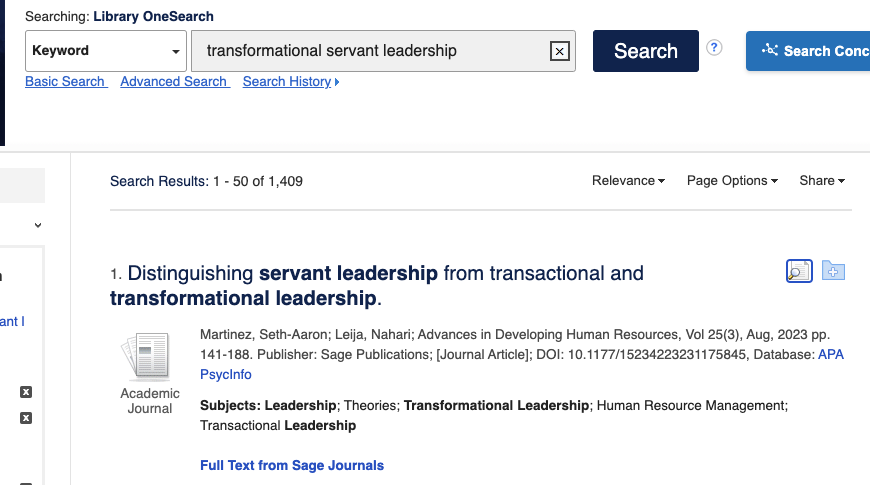
\includegraphics{assets/u2/library1.png}

\end{figure}%

Click the ``Export'' button on the right side, then choose ``Direct
Export in RIS Format,'' then ``Save.''

\begin{figure}

\caption{\label{fig-library2}Screenshot of TWU Library Search Results
Showing Export Button (Circled)}

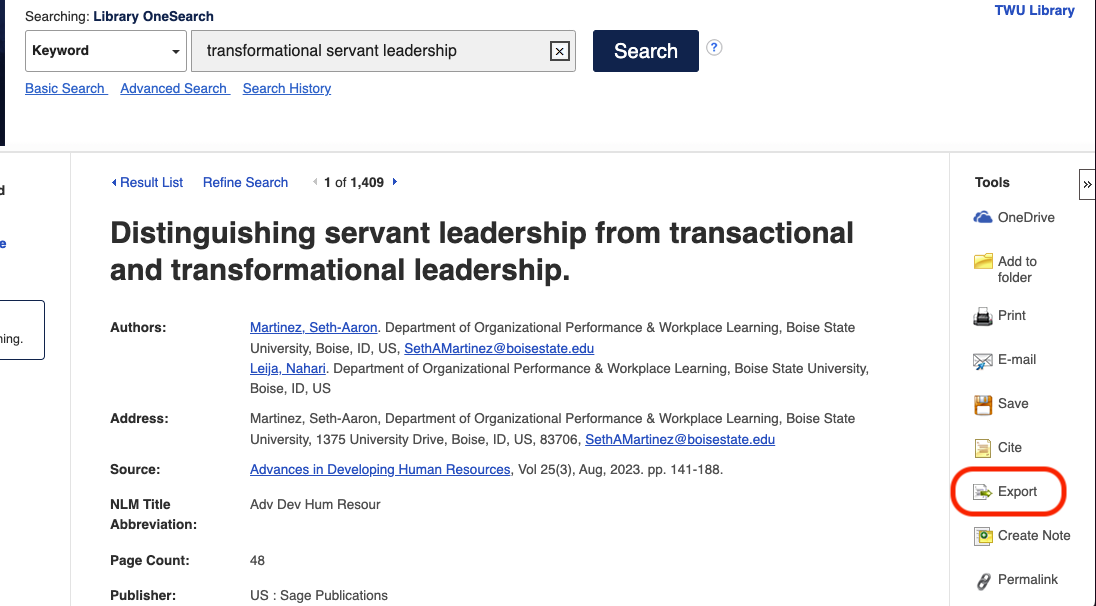
\includegraphics{assets/u2/library2.png}

\end{figure}%

\begin{figure}

\caption{\label{fig-library3}Screenshot of TWU Library Export Manager
File Format Options (RIS Selected)}

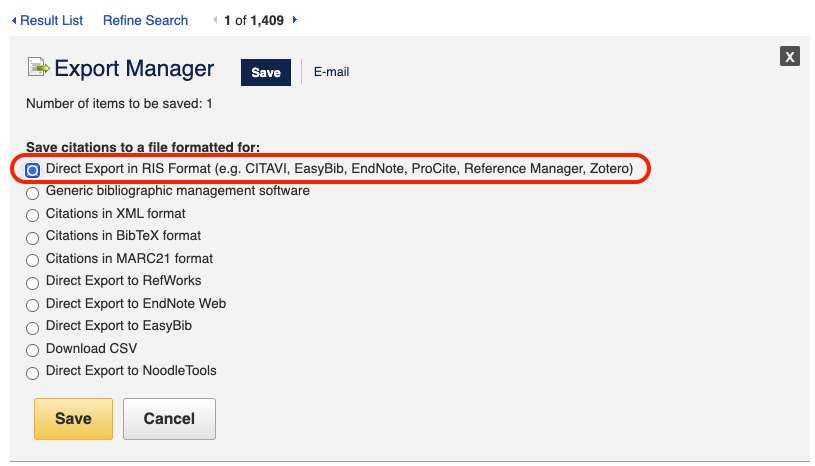
\includegraphics{assets/u2/library3.png}

\end{figure}%

You might get a message to install the Zotero Connector in your browser,
go ahead and do that. Once you have imported the reference, you will
have a brand new item in your Zotero library!

From here on to the day you graduate, Zotero will be with you and you
may find yourself using it every day. It is absolutely indispensable.

\subsection{Activity: Using Zotero}\label{activity-using-zotero}

\begin{tcolorbox}[enhanced jigsaw, toprule=.15mm, colback=white, colframe=quarto-callout-note-color-frame, bottomtitle=1mm, leftrule=.75mm, coltitle=black, titlerule=0mm, rightrule=.15mm, colbacktitle=quarto-callout-note-color!10!white, left=2mm, title={Learning Activity}, opacitybacktitle=0.6, opacityback=0, breakable, toptitle=1mm, arc=.35mm, bottomrule=.15mm]

Now that you have connected LitMaps to Zotero, let's explore how to use
Zotero in your studies.

\begin{itemize}
\tightlist
\item
  \textbf{Watch}: review the basics of Zotero by watching
  \href{https://www.youtube.com/watch?v=5xClqW2Jv04}{\emph{What is
  Zotero?}} (2019)
\end{itemize}

\url{https://www.youtube-nocookie.com/embed/5xClqW2Jv04}

Now, let's start using it. Go to LitMaps, TWU Library, or Google Scholar
and find articles that interest you. Populate your library with the
following resources to support a research topic that interests you.

\begin{itemize}
\tightlist
\item
  manual entry for a published book
\item
  manual entry for a chapter within an edited book (note that the
  library record for a book section or chapter should have separate
  fields for the author(s) and editor(s))
\item
  automatic harvesting of bibliographic information for a journal
  article (if supported by a browser extension or bookmarklet by your
  preferred citation management tool)
\item
  automatic harvesting of bibliographic information for a newspaper
  article (if supported by a browser extension or bookmarklet by your
  preferred citation management tool)
\item
  \textbf{Review}: In each case review that all relevant fields required
  for the bibliography have been completed correctly. Don't rely on the
  accuracy of the automatic features as they are dependent on the
  metadata and adherence to open standards on the source website. Pay
  particular attention to punctuation and consistent use of
  capitalization.
\item
  add descriptive tags; this will enhance searching of your library
  database
\item
  organize your resources using folders
\end{itemize}

Next, experiment with some of the Zotero annotation features.

\begin{itemize}
\tightlist
\item
  \textbf{Watch:}
  \href{https://www.youtube.com/watch?v=lGeJCsNHBR4}{\emph{How to
  Annotate PDFs in Zotero}} (2023) for instructions.
\end{itemize}

\url{https://www.youtube-nocookie.com/embed/lGeJCsNHBR4}

If you want to take the next step, let's make your tools work together.

\begin{itemize}
\tightlist
\item
  \textbf{Watch} the
  \href{https://www.youtube.com/watch?v=CGGeMrtyjBI?}{video} on Zotero
  and Obsidian integration (2022) and see the features offered when you
  integrate these tools.
\end{itemize}

\url{https://www.youtube-nocookie.com/embed/CGGeMrtyjBI}

\begin{itemize}
\tightlist
\item
  \textbf{Write}: about your learning process and how you might use
  Zotero or another citation management tool in your studies.
\end{itemize}

\end{tcolorbox}

\section{Openness in Education}\label{openness-in-education}

At this point in the unit you have used various tools to discover and
curate resources. In this topic we would like to introduce you to a
value in education that we believe is important for creating a true
community of inquiry in higher education. If you haven't already noticed
from the title of this topic, we are thinking about \emph{openness}.
Here is a quick overview from the OER Foundation:
\emph{\href{https://vimeo.com/557927481}{Open Access Explained}} (2021).

\href{https://vimeo.com/557927481}{Watch video}

And here is an article you can read (for free) from the British
organization Wonkhe.

Open educational resources, or OER, refers to freely accessible and
openly licensed educational materials that can be used, shared, and
modified without cost. These resources include a variety of digital
assets such as textbooks, lecture notes, multimedia content, and
assessment tools. The key features of OER include their open licenses,
which typically allow users to \textbf{\emph{retain, reuse, revise,
remix}}, and \textbf{\emph{redistribute}} the content (Wiley, n.d.).

\subsubsection*{The 5 Rs of Openness}\label{the-5-rs-of-openness}
\addcontentsline{toc}{subsubsection}{The 5 Rs of Openness}

\textbf{Retain} the right to make, own, and control copies of the
content

\textbf{Reuse} the right to use the content in a wide range of ways
(e.g., in a class, in a study group, on a website, in a video)

\textbf{Revise} the right to adapt, adjust, modify, or alter the content
itself (e.g., translate the content into another language)

\textbf{Remix} the right to combine the original or revised content with
other open content to create something new (e.g., incorporate the
content into a mashup)

\textbf{Redistribute} the right to share copies of the original content,
your revisions, or your remixes with others (e.g., give a copy of the
content to a friend)

\begin{tcolorbox}[enhanced jigsaw, toprule=.15mm, colback=white, colframe=quarto-callout-note-color-frame, arc=.35mm, opacityback=0, breakable, rightrule=.15mm, bottomrule=.15mm, leftrule=.75mm, left=2mm]

Note that this material was created and published freely under a
Creative Commons Attribution 4.0 license.

\end{tcolorbox}

Why use OER? The usefulness of OER in higher education can be attributed
to several compelling reasons:

\begin{itemize}
\tightlist
\item
  \textbf{Affordability}: OER mitigates financial barriers for students
  by providing access to educational materials at no cost. This is
  particularly significant as the high cost of traditional textbooks and
  learning resources can be a substantial financial burden for students.
\item
  \textbf{Accessibility}: OER promotes equitable access to educational
  content globally. Anyone with an internet connection can benefit from
  OER, fostering inclusivity and addressing issues of accessibility in
  higher education.
\item
  \textbf{Customized learning materials}: Instructors can tailor OER to
  align seamlessly with course requirements, creating a personalized
  learning experience for students.
\item
  \textbf{Community collaboration}: OER encourages collaborative
  knowledge sharing among educators and students, fostering a sense of
  shared learning within the academic community.
\item
  \textbf{Current and relevant content}: the adaptable nature of OERs
  facilitates easy updates, ensuring educational materials reflect the
  latest advancements, and providing students with up-to-date
  information.
\item
  \textbf{Global perspectives}: The inclusive design of OER integrates
  diverse global viewpoints, enhancing cultural awareness and expanding
  students' understanding of various academic frameworks.
\item
  \textbf{Ethical usage}: OER operates with transparent licensing,
  ensuring ethical use of materials and upholding the principles of
  academic integrity.
\end{itemize}

In summary, OER offers a cost effective, flexible, and collaborative
approach to educational resource development, making it a valuable and
impactful asset in higher education. Its adoption aligns with the
broader goals of enhancing accessibility, affordability, and inclusivity
in the learning experience.

\subsection{Activity: Finding OERs}\label{activity-finding-oers}

\begin{tcolorbox}[enhanced jigsaw, toprule=.15mm, colback=white, colframe=quarto-callout-note-color-frame, bottomtitle=1mm, leftrule=.75mm, coltitle=black, titlerule=0mm, rightrule=.15mm, colbacktitle=quarto-callout-note-color!10!white, left=2mm, title={Learning Activity}, opacitybacktitle=0.6, opacityback=0, breakable, toptitle=1mm, arc=.35mm, bottomrule=.15mm]

Go to the \href{https://libguides.twu.ca/oer}{Open Educational Resources
Libguide} from the TWU Library.

\begin{itemize}
\item
  \textbf{Watch}:
\item
  \href{https://www.youtube.com/watch?v=Hkz4q2yuQU8}{\emph{How to use
  OER}} (2012), then browse through the categories of OERs by discipline
  provided. Take some time to find an OER that relates to a topic that
  interests you.
\item
  \textbf{Write}: Create an entry in Obsidian about an OER resource you
  found. Use the CRAAP test to evaluate it and explain why this resource
  interests you.
\end{itemize}

\end{tcolorbox}

\subsection{Activity: Advocating for
OER}\label{activity-advocating-for-oer}

\begin{tcolorbox}[enhanced jigsaw, toprule=.15mm, colback=white, colframe=quarto-callout-note-color-frame, bottomtitle=1mm, leftrule=.75mm, coltitle=black, titlerule=0mm, rightrule=.15mm, colbacktitle=quarto-callout-note-color!10!white, left=2mm, title={Learning Activity}, opacitybacktitle=0.6, opacityback=0, breakable, toptitle=1mm, arc=.35mm, bottomrule=.15mm]

So how do open educational resources affect you as a student? Why should
you care? We've shared some of the benefits of openness in education,
but there are several other reasons OER benefit students.

\begin{itemize}
\tightlist
\item
  \textbf{Watch}:
\item
  \href{https://www.youtube.com/watch?v=SX0K0hb_xKE}{\emph{A Review of
  the Effectiveness \& Perceptions of Open Educational Resources as
  Compared to Textbooks}} (2016)
\end{itemize}

\url{https://www.youtube-nocookie.com/embed/SX0K0hb_xKE}

\begin{itemize}
\tightlist
\item
  \textbf{Read}: For more information on OER Advocacy, see the chapter
  on
  \href{https://opentextbc.ca/studenttoolkit/chapter/step-three-how-to-advocate-on-your-campus/}{How
  to Advocate on Your Campus} in the OER Student Toolkit.
\item
  \textbf{Write}: Create an entry in Obsidian about the benefits of
  OERs.
\end{itemize}

\end{tcolorbox}

\subsection{Activity: Reflecting on Your
Resources}\label{activity-reflecting-on-your-resources}

\begin{tcolorbox}[enhanced jigsaw, toprule=.15mm, colback=white, colframe=quarto-callout-note-color-frame, bottomtitle=1mm, leftrule=.75mm, coltitle=black, titlerule=0mm, rightrule=.15mm, colbacktitle=quarto-callout-note-color!10!white, left=2mm, title={Learning Activity}, opacitybacktitle=0.6, opacityback=0, breakable, toptitle=1mm, arc=.35mm, bottomrule=.15mm]

We've reached the end of Unit 2, where you have explored several tools
and practiced digital skills to help you find and select resources for
academic study. As you have practiced the activities in this unit, you
have curated resources about the topic of your choice. In this activity
we ask you to write a paragraph about this topic, utilizing the
resources you have found.

\begin{itemize}
\item
  \textbf{Read}:
  \href{https://writingcenter.unc.edu/tips-and-tools/paragraphs/}{This
  resource} on how to write a good paragraph published by the
  University of North Carolina at Chapel Hill. For more writing tips
  see the
  \href{https://create.twu.ca/learningcommons/writing-resources/?_gl=1*1uail9b*_ga*NDk4NDk0OTI0LjE3MTY5MTYzNTc.*_ga_NZ4GVM10JT*MTcyNTY2MjM0My4xMTYuMS4xNzI1NjYyMzcwLjMzLjAuMA..}{Writing
  Resources website} from the TWU Learning Commons.
\item
  \textbf{Write}: Draft a paragraph on an issue relating to your
  research topic. Your paragraph must contain:
\item
  a verbatim quote from one of your sources
\item
  a paraphrased fact from one of your sources

  Use the features of your citation management software to integrate:
\item
  the in-text reference for your verbatim quotation
\item
  the in-text reference for the paraphrased fact
\item
  the automatically generated reference list using APA style (consult
  the Quick APA Guide to review your formatting)
\end{itemize}

Generate a PDF version of your paragraph.

\begin{itemize}
\tightlist
\item
  \textbf{Reflect}: Prepare a short journal entry of about 150 words
  sharing your experiences in using citation management software. For
  example: What worked well? Did you struggle with any of the
  instructions? Did you learn any new skills?
\end{itemize}

Note that this reflection can be used for your assessment in this
course.

\end{tcolorbox}

\subsection{Activity: Annotated
Bibliography}\label{activity-annotated-bibliography}

\begin{tcolorbox}[enhanced jigsaw, toprule=.15mm, colback=white, colframe=quarto-callout-note-color-frame, bottomtitle=1mm, leftrule=.75mm, coltitle=black, titlerule=0mm, rightrule=.15mm, colbacktitle=quarto-callout-note-color!10!white, left=2mm, title={Learning Activity}, opacitybacktitle=0.6, opacityback=0, breakable, toptitle=1mm, arc=.35mm, bottomrule=.15mm]

In this activity you will create an annotated bibliography related to a
research topic of your choice.

\begin{itemize}
\tightlist
\item
  \textbf{Read} the following resources:

  \begin{itemize}
  \tightlist
  \item
    Evaluating online sources:
    \href{https://www.science.org/content/article/how-seriously-read-scientific-paper?v=sy9PVZAbSAQ}{\emph{How
    to (Seriously) Read an Academic Paper}} (2016)
  \item
    Preparing an annotated bibliography:
    \href{https://library.concordia.ca/help/writing/annotated-bibliography.php}{\emph{Writing
    an Annotated Bibliography}} (n.d.) and
    \emph{\href{https://library.concordia.ca/help/writing/annotated-bibliography.php\#:~:text=In\%20an\%20annotated\%20bibliography\%2C\%20each,relevance\%20to\%20your\%20paper\%20topic.}{How
    to Write an Annotated Bibliography}} (2022)
  \item
    \emph{\href{https://owl.purdue.edu/owl/general_writing/common_writing_assignments/annotated_bibliographies/annotated_bibliography_samples.html}{Annotated
    Bibliography Samples: Purdue Owl}} (n.d.-a)
  \end{itemize}
\item
  \textbf{Annotate}: Next, create an annotated bibliography in Obsidian
  for two sources---include a journal article and a book chapter from an
  edited collection of chapters by multiple authors.

  \begin{itemize}
  \tightlist
  \item
    You can select resources already saved in your library or search for
    new ones in support of your research topic.
  \item
    Use the note or comment feature of your citation management software
    to record a copy of your annotation.
  \item
    You must use Zotero to generate the references using APA format.
  \end{itemize}
\end{itemize}

\end{tcolorbox}

\section*{Summary}\label{summary-1}
\addcontentsline{toc}{section}{Summary}

\markright{Summary}

In this unit, you have had the opportunity to develop crucial skills for
navigating the digital resource landscape. You are now able to
effectively find and evaluate resources, manage citations, and
understand the importance of openness in education. These skills will
enhance your ability to use digital resources for academic and
professional growth responsibly and effectively.

In addition, exploring openness in education broadened your
understanding of the transformative power of freely accessible
educational resources. By delving into the principles of open
educational resources (OER) and open access, we hope to have conveyed
their significance in making education more accessible. This newfound
awareness not only empowers you as a learner but also places you in a
role as a contributor to a global academic community. As you conclude
this unit with refined skills in resource navigation, citation
management, and a deeper appreciation for openness in education, you are
well equipped to responsibly and effectively leverage digital resources
for ongoing academic and professional growth. These skills are not just
tools for immediate success, but enduring assets, shaping your lifelong
journey in the ever evolving realm of digital knowledge.

\begin{tcolorbox}[enhanced jigsaw, toprule=.15mm, colback=white, colframe=quarto-callout-note-color-frame, bottomtitle=1mm, leftrule=.75mm, coltitle=black, titlerule=0mm, rightrule=.15mm, colbacktitle=quarto-callout-note-color!10!white, left=2mm, title={Checking Your Learning}, opacitybacktitle=0.6, opacityback=0, breakable, toptitle=1mm, arc=.35mm, bottomrule=.15mm]

Before you move on to the next unit check that you are able to:

\begin{itemize}
\tightlist
\item
  describe your engagement with digital technology
\item
  apply digital tools to support learning in an academic environment
\item
  explain what digital literacies mean for you in a tertiary education
  context
\item
  examine your digital footprint
\item
  build your professional online biography
\item
  examine privacy concerns related to various platforms and tools
\item
  describe how to protect yourself, and other students and colleagues,
  to stay safe in the digital environment
\end{itemize}

\end{tcolorbox}

\bookmarksetup{startatroot}

\chapter{Connecting Ideas for
Learning}\label{connecting-ideas-for-learning}

\section*{Overview}\label{overview-2}
\addcontentsline{toc}{section}{Overview}

\markright{Overview}

Welcome to our third unit in \emph{Learning with Technology}, where we
explore the symbiotic relationship between technology and knowledge
synthesis. In this unit we will unravel the intricacies of sense-making
through hyperlinks and tags, discovering their pivotal roles in creating
a cohesive web of information. You will delve into the transformative
realm of digital note taking, learning how to capture, organize, and
review key ideas efficiently. As we progress we will unlock the
potential of visual representations through concept maps, using digital
tools to illustrate complex relationships and hierarchies that foster a
deeper understanding of interconnected ideas. Moreover, we'll venture
into a curated selection of digital tools designed to support and
augment the learning process, evaluating their benefits in catering to
diverse learning styles and preferences. By the conclusion of this unit
you will not only have mastered the art of connecting ideas through
hyperlinks, tags, note taking, and concept maps, but you will also be
equipped with a toolkit of digital resources to enrich your learning
journey.

\subsection*{Topics}\label{topics-2}
\addcontentsline{toc}{subsection}{Topics}

This unit is divided into the following topics:

\begin{enumerate}
\def\labelenumi{\arabic{enumi}.}
\tightlist
\item
  Sense-making through hyperlinks
\item
  Sense-making through tags
\item
  Note taking
\item
  Concept maps
\item
  Digital tools to support learning
\end{enumerate}

\subsection*{Learning Outcomes}\label{learning-outcomes-1}
\addcontentsline{toc}{subsection}{Learning Outcomes}

When you have completed this unit you will be able to:

\begin{itemize}
\tightlist
\item
  Build and customize technology integrated workflows to enhance and
  enrich your learning journey
\item
  Practice evaluative judgment to document your process of learning in
  complex domains of knowledge
\item
  Evaluate digital tools, platforms, and interactions based on ethical
  principles
\end{itemize}

\subsection*{Activity Checklist}\label{activity-checklist-2}
\addcontentsline{toc}{subsection}{Activity Checklist}

Here is a checklist of learning activities you will benefit from in
completing this unit. You may find it useful for planning your work.

\textbf{Learning Activities}

\begin{itemize}
\tightlist
\item
  Practice using links and tags to connect your ideas in Obsidian
\item
  Write a reflective post on your learning experiences
\item
  Practice various note taking skills
\end{itemize}

\begin{tcolorbox}[enhanced jigsaw, toprule=.15mm, colback=white, colframe=quarto-callout-note-color-frame, arc=.35mm, opacityback=0, breakable, rightrule=.15mm, bottomrule=.15mm, leftrule=.75mm, left=2mm]

\emph{Note: Working through course activities will help you to meet the
learning outcomes and successfully complete your assessments.}

\end{tcolorbox}

:::

\begin{tcolorbox}[enhanced jigsaw, toprule=.15mm, colback=white, colframe=quarto-callout-note-color-frame, arc=.35mm, opacityback=0, breakable, rightrule=.15mm, bottomrule=.15mm, leftrule=.75mm, left=2mm]

\textbf{Assessment}

\begin{itemize}
\tightlist
\item
  Please see the Assessment section in Moodle for assignment details.
\end{itemize}

\end{tcolorbox}

\subsection*{Resources}\label{resources-2}
\addcontentsline{toc}{subsection}{Resources}

\begin{itemize}
\tightlist
\item
  All resources will be provided online in the unit.
\end{itemize}

\section{Sense-making Through
Hyperlinks}\label{sense-making-through-hyperlinks}

In higher education, your task is to build on the skills you bring from
your previous experience and apply those skills in a much more focused
field of study. Previously, you might have been able to succeed in
school by having a great memory, but increasingly, you will be asked to
do much more. You will be required to understand the theoretical basis
of ideas (analysis) and also make connections between ideas to create
new ideas (synthesis). This may feel challenging at first, but you will
learn.

One of the challenges is that there is simply far too much information
for you to analyze for any task that you might need to do for an
instructor. In a previous unit, you learned some basic skills in finding
and managing resources that you will need and in this unit, you will
learn some ways to begin to analyze and synthesize information and
documents in a systematic way.

If you learn this workflow well and learn how to customize it to your
needs (that's synthesis), you will be ahead of the game when it comes
time to complete papers in other courses.

The key to this component of your workflow is the lowly
\href{https://en.wikipedia.org/wiki/Hyperlink}{hyperlink}. You'll know
that if you click or tap that highlighted word you will be taken to
another website, in this case, the Wikipedia article on hyperlinks. That
is a hyperlink and it is the most basic unit of the entire internet,
which is simply a massive collection of documents all linked together.
At its most basic form, a hyperlink is simply a connection between two
documents where a hyperlink in one document allows you to open the
second document.

In this workflow instead of just linking two documents together you will
link two ideas together (by linking documents). Your Obsidian vault is
essentially a website that is only accessible on your computer; instead
of links going to documents on other servers, you link to documents
within the vault (although you can still link to the web).

\subsection*{Linking in Obsidian}\label{linking-in-obsidian}
\addcontentsline{toc}{subsection}{Linking in Obsidian}

There are two methods of building hyperlinks in Obsidian: Wikilinks and
markdown links, and we will cover both here.

\subsubsection*{Wikilinks}\label{wikilinks}
\addcontentsline{toc}{subsubsection}{Wikilinks}

A Wikilink, the default in Obsidian, is really simple to build. All you
have to do is type two opening square brackets, like this
\texttt{{[}{[}}, and Obsidian will do a couple things automatically.
First, Obsidian will create the closing brackets to match, so you end up
with this \texttt{{[}{[}{]}{]}}, with your cursor in the middle, and
second, Obsidian will present a list of all the pages in your vault,
from which you can choose the page you want linked.

{[}Alt text: {]}

\begin{figure}

\caption{\label{fig-wikilink}Screenshot, Create a Wikilink in Obsidian}

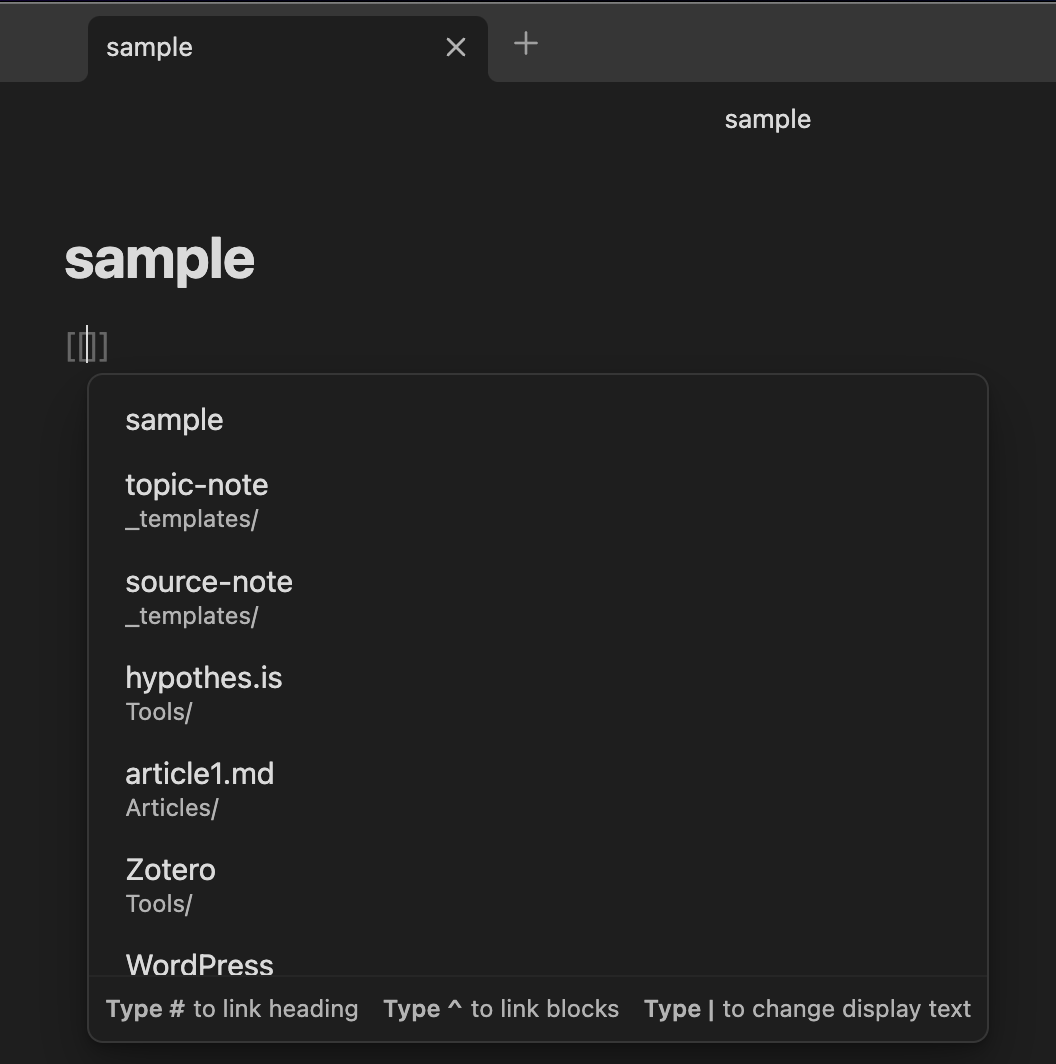
\includegraphics{assets/u3/wikilink.png}

\end{figure}%

Once you choose a page (in this case, article1.md), Obsidian will do the
rest, and you will end up with this view:

\begin{figure}

\caption{\label{fig-wikilink2}Screenshot, Wikilink Created in Obsidian}

\centering{

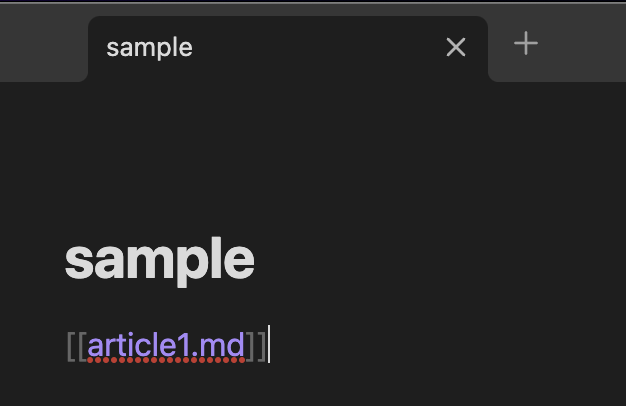
\includegraphics{assets/u3/wikilink2.png}

}

\end{figure}%

From Hypothes.is you can create a link to Zotero. By pressing and
holding the ``Command'' (macOS) or ``CTRL'' (Windows) button on the
keyboard and then hovering over the link you've created, you will get a
preview of the Zotero page. If you press and hold the ``Command''
(macOS) or ``CTRL'' (Windows) button on the keyboard and then click the
link, you will be taken to the page. Once on the Zotero page, you can
scroll to the bottom of the page and see ``Backlinks'' (a link back to
the original page). If you don't see backlinks, click the three dots in
the top right corner of the page and choose ``Backlinks in document.''

\subsubsection*{Markdown Links}\label{markdown-links}
\addcontentsline{toc}{subsubsection}{Markdown Links}

While Wikilinks are the default in Obsidian and are the easiest way to
link within your vault, sometimes you might want to link to a site on
the web. The syntax for a markdown link is a bit different but is still
very simple. There are two parts you need to remember:

\begin{itemize}
\tightlist
\item
  the link text (this is what you want your reader to see on your page)
\item
  the link URL (this is the web address of the site you want them to
  visit)
\end{itemize}

Here is the syntax:
\texttt{{[}Link\ text\ between\ single\ square\ brackets{]}(URL\ inside\ parentheses)\{target="\_blank"\}\ So\ if\ you\ want\ someone\ to\ see\ the\ word\ "YouTube"\ on\ the\ page\ and\ for\ them\ to\ be\ taken\ to\ the\ YouTube\ website\ when\ they\ click\ the\ link,\ the\ syntax\ would\ be}\href{https://youtube.com}{YouTube}`
which will display like this: \href{https://youtube.com}{YouTube}.
Notice that there are no spaces between the closing square bracket and
the opening parenthesis.

Here is the syntax:
\texttt{{[}Link\ text\ between\ single\ square\ brackets{]}(URL\ inside\ parentheses)\{target="\_blank"\}}
So if you want someone to see the word ``YouTube'' on the page and for
them to be taken to the YouTube website when they click the link, the
syntax would be
\texttt{{[}YouTube{]}(https://youtube.com)\{target="\_blank"\}} which
will display like this: \href{https://youtube.com}{YouTube}. Notice that
there are no spaces between the closing square bracket and the opening
parenthesis.

\subsection*{Why Link?}\label{why-link}
\addcontentsline{toc}{subsection}{Why Link?}

Creating links to other related topics in your notes is a way that you
can start to build connections in your mind about how different ideas
are related. For example, if you are studying ``trees,'' you might want
to link over to the previous notes that you created on ``plants,''
``forests,'' or ``climate change.'' During your study on trees, you
might want to create notes on ``deciduous'' and ``coniferous'' trees, or
``xylem'' and ``phloem,'' and link those articles to ``trees.'' By
continually linking notes that are related you are creating a web of
your knowledge as well as reminders of how ideas are related. Linking is
a way for you to make sense of the information that is coming into your
consciousness.

Once you have created links between different files in your vault you
can visualize these links using the ``Graph View'' in Obsidian. Here is
part of the graph view for a major paper. Each of the white dots
represents a file in the vault, and their size is relative to the number
of pages linked to that article. You can see that there are three really
big pages that have many links. Those are clearly very important pages.

\begin{figure}

\caption{\label{fig-graph2}Screenshot, Graph View for Linked Documents
in Obsidian}

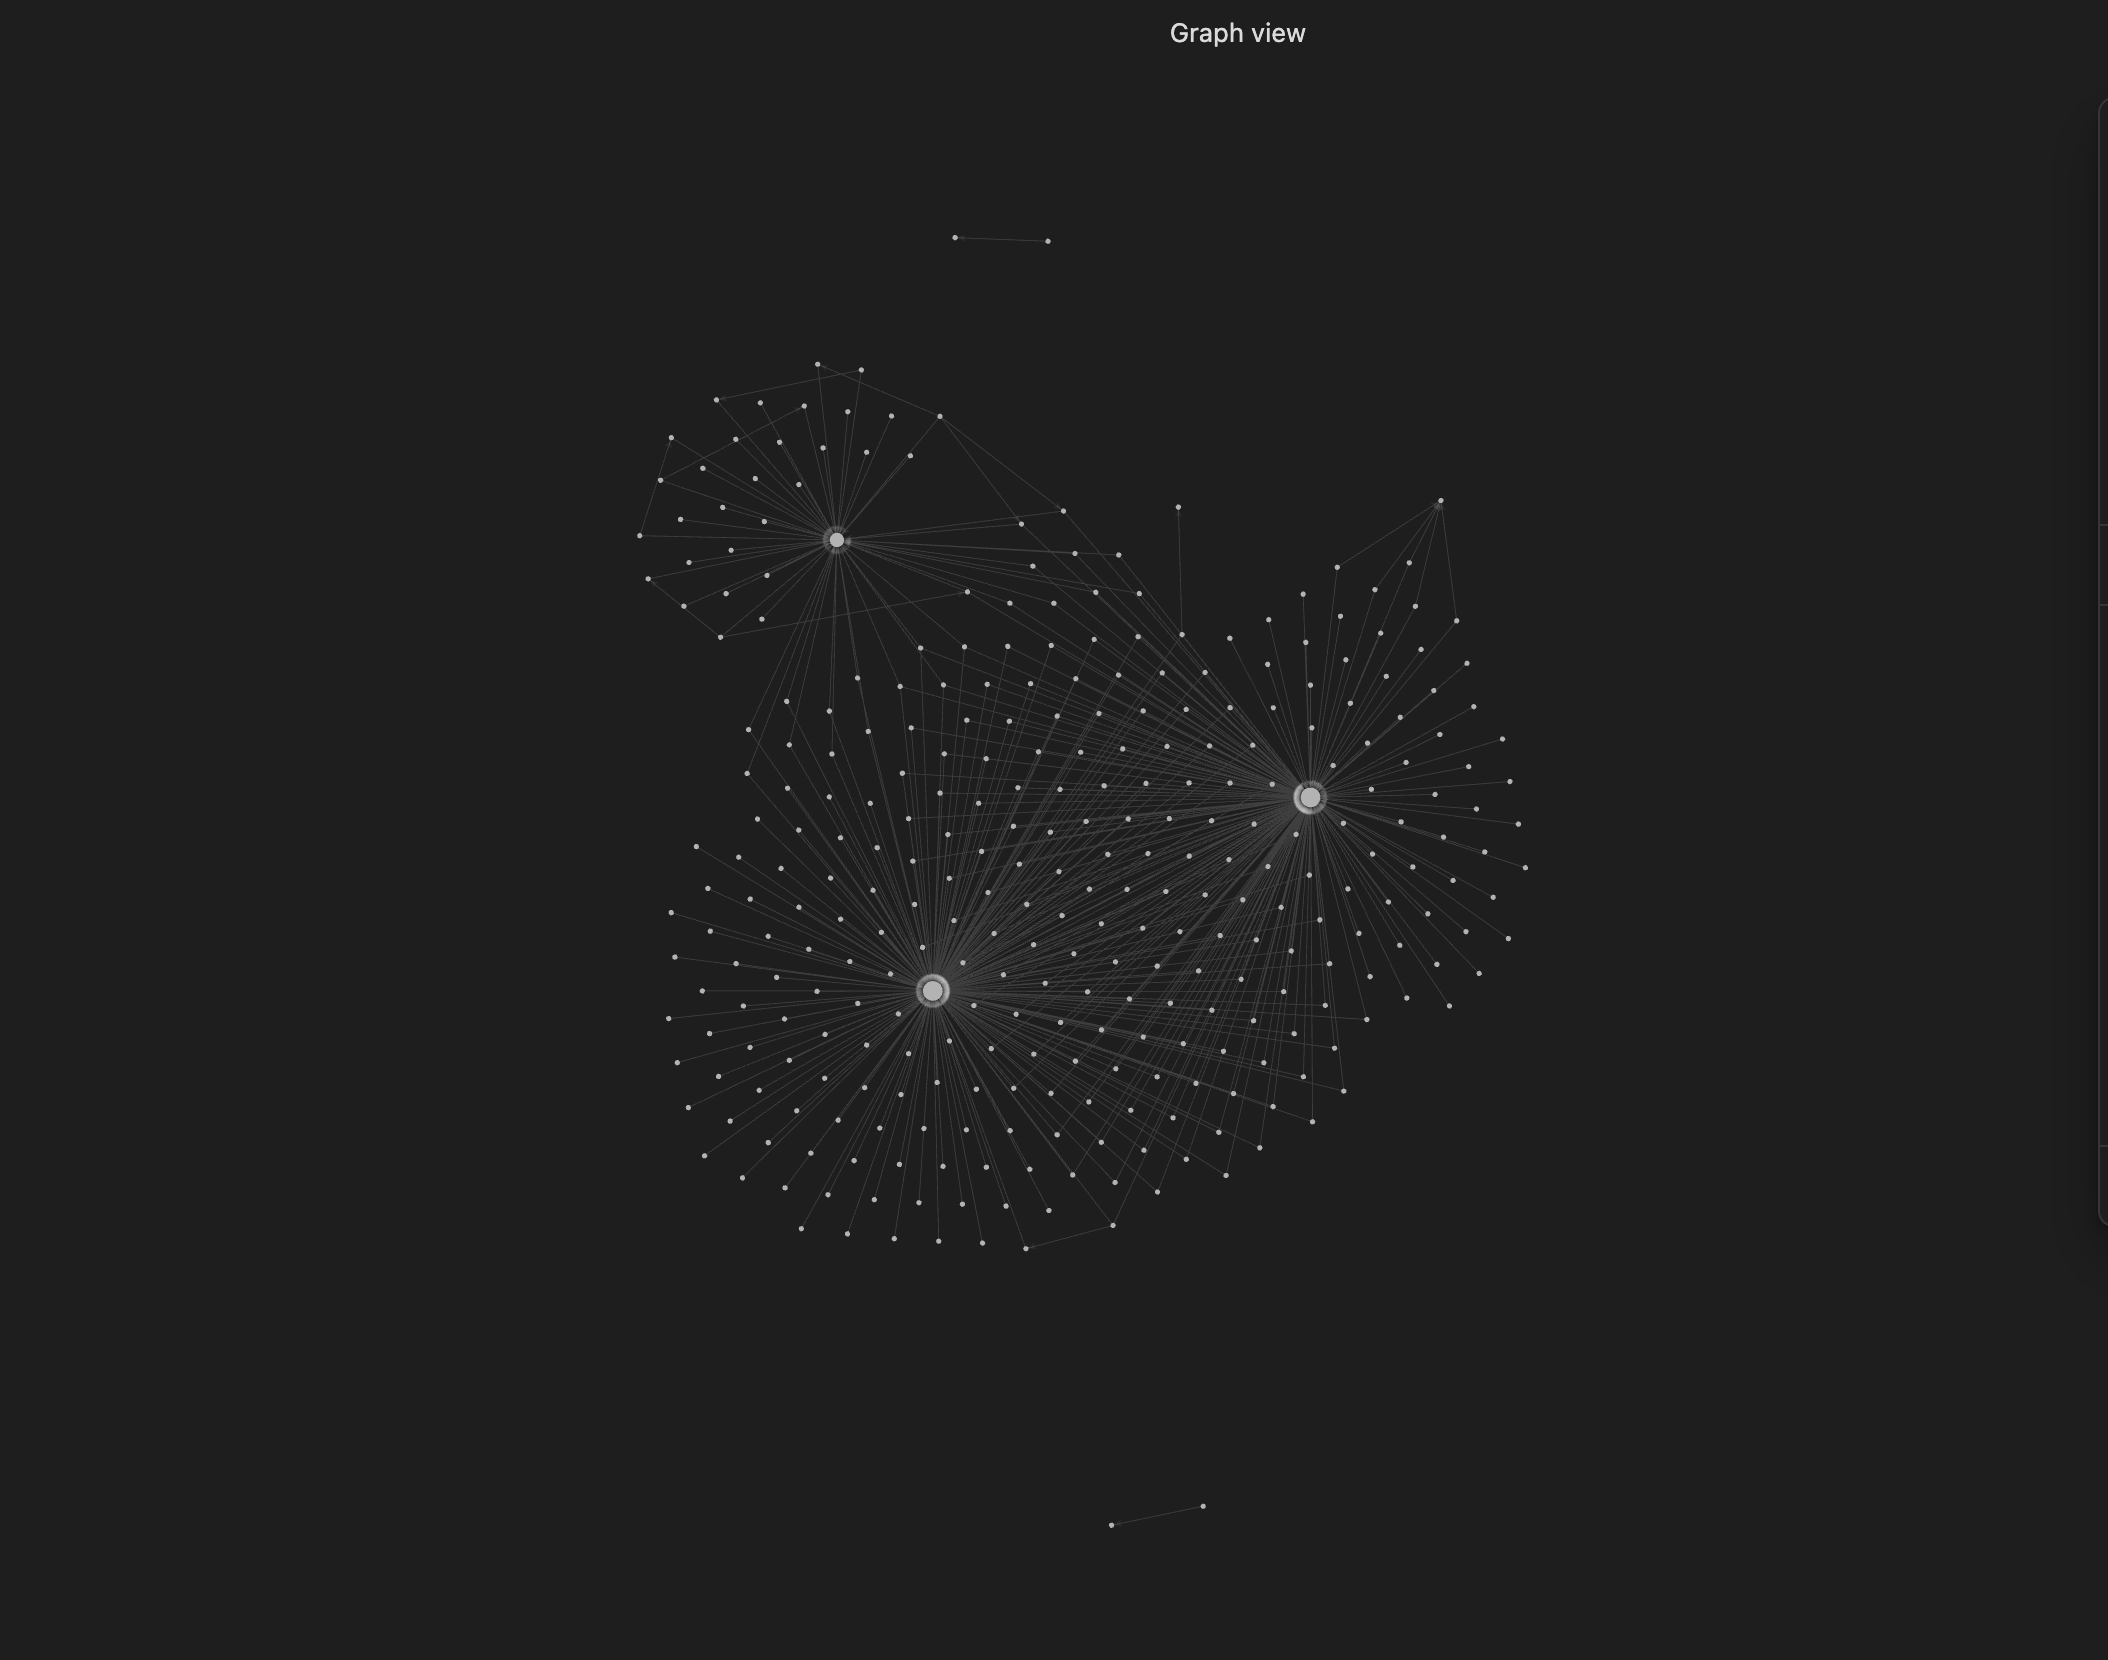
\includegraphics{assets/u3/graph2.png}

\end{figure}%

\subsection{Activity: Link, Connect, and
Reflect}\label{activity-link-connect-and-reflect}

\begin{tcolorbox}[enhanced jigsaw, toprule=.15mm, colback=white, colframe=quarto-callout-note-color-frame, bottomtitle=1mm, leftrule=.75mm, coltitle=black, titlerule=0mm, rightrule=.15mm, colbacktitle=quarto-callout-note-color!10!white, left=2mm, title={Learning Activity}, opacitybacktitle=0.6, opacityback=0, breakable, toptitle=1mm, arc=.35mm, bottomrule=.15mm]

\begin{itemize}
\item
  \textbf{Link}: Follow the directions above to add notes to Obsidian on
  a topic of interest. Search online for interesting articles and videos
  you want to add to your notes and practice adding them using Wikilinks
  and markdown links. Locate the graph view in Obsidian to see the
  connections between the ideas you've added.
\item
  \textbf{Write}: After spending some time practicing this new skill,
  write a reflective journal entry on the process you followed and what
  your experience was like. What did you struggle with? How did you
  troubleshoot? What are the advantages of organizing your notes using
  this method?
\end{itemize}

Feel free to discuss your experience on the
\href{https://twu.discourse.group/auth/microsoft_office365}{Learning
Hub} in Discourse. You can also post any questions you have about this
process and get technical support from your instructors and
facilitators.

\end{tcolorbox}

\section{Sense-making Through Tags}\label{sense-making-through-tags}

A tag is a very short, descriptive word or phrase you can apply to an
idea. You are likely familiar with the idea of a hashtag
(\texttt{\#\textasciigrave{}\textasciigrave{})} from various social
media apps as a way to quickly find information on a specific topic. A
tag in Obsidian works just like a hashtag in social media. If you type
\texttt{\#trees} on a file about trees, and then do the same on your
pages about xylem, phloem, climate change, plants, forests, deciduous,
and coniferous, you could click that tag on any one of those pages, and
Obsidian will find every page that contains that tag.

This acts like a super-fast search of your notes for a particular topic
or ideas related to a topic.

We recommend that you put your tags in the same spot on each page so you
know where to find them. You can also put those tags at any place in
your notes and Obsidian will show you the specific spot in your notes
where the tag lives.

You can also show tags in your graph view, as below. Green dots are tags
and white dots are files (as before). You can see in this image that
there are many more connections.

\begin{figure}

\caption{\label{fig-graph1}Screenshot, Graph View in Obsidian Including
Files (White Dots) and Tags (Green Dots)}

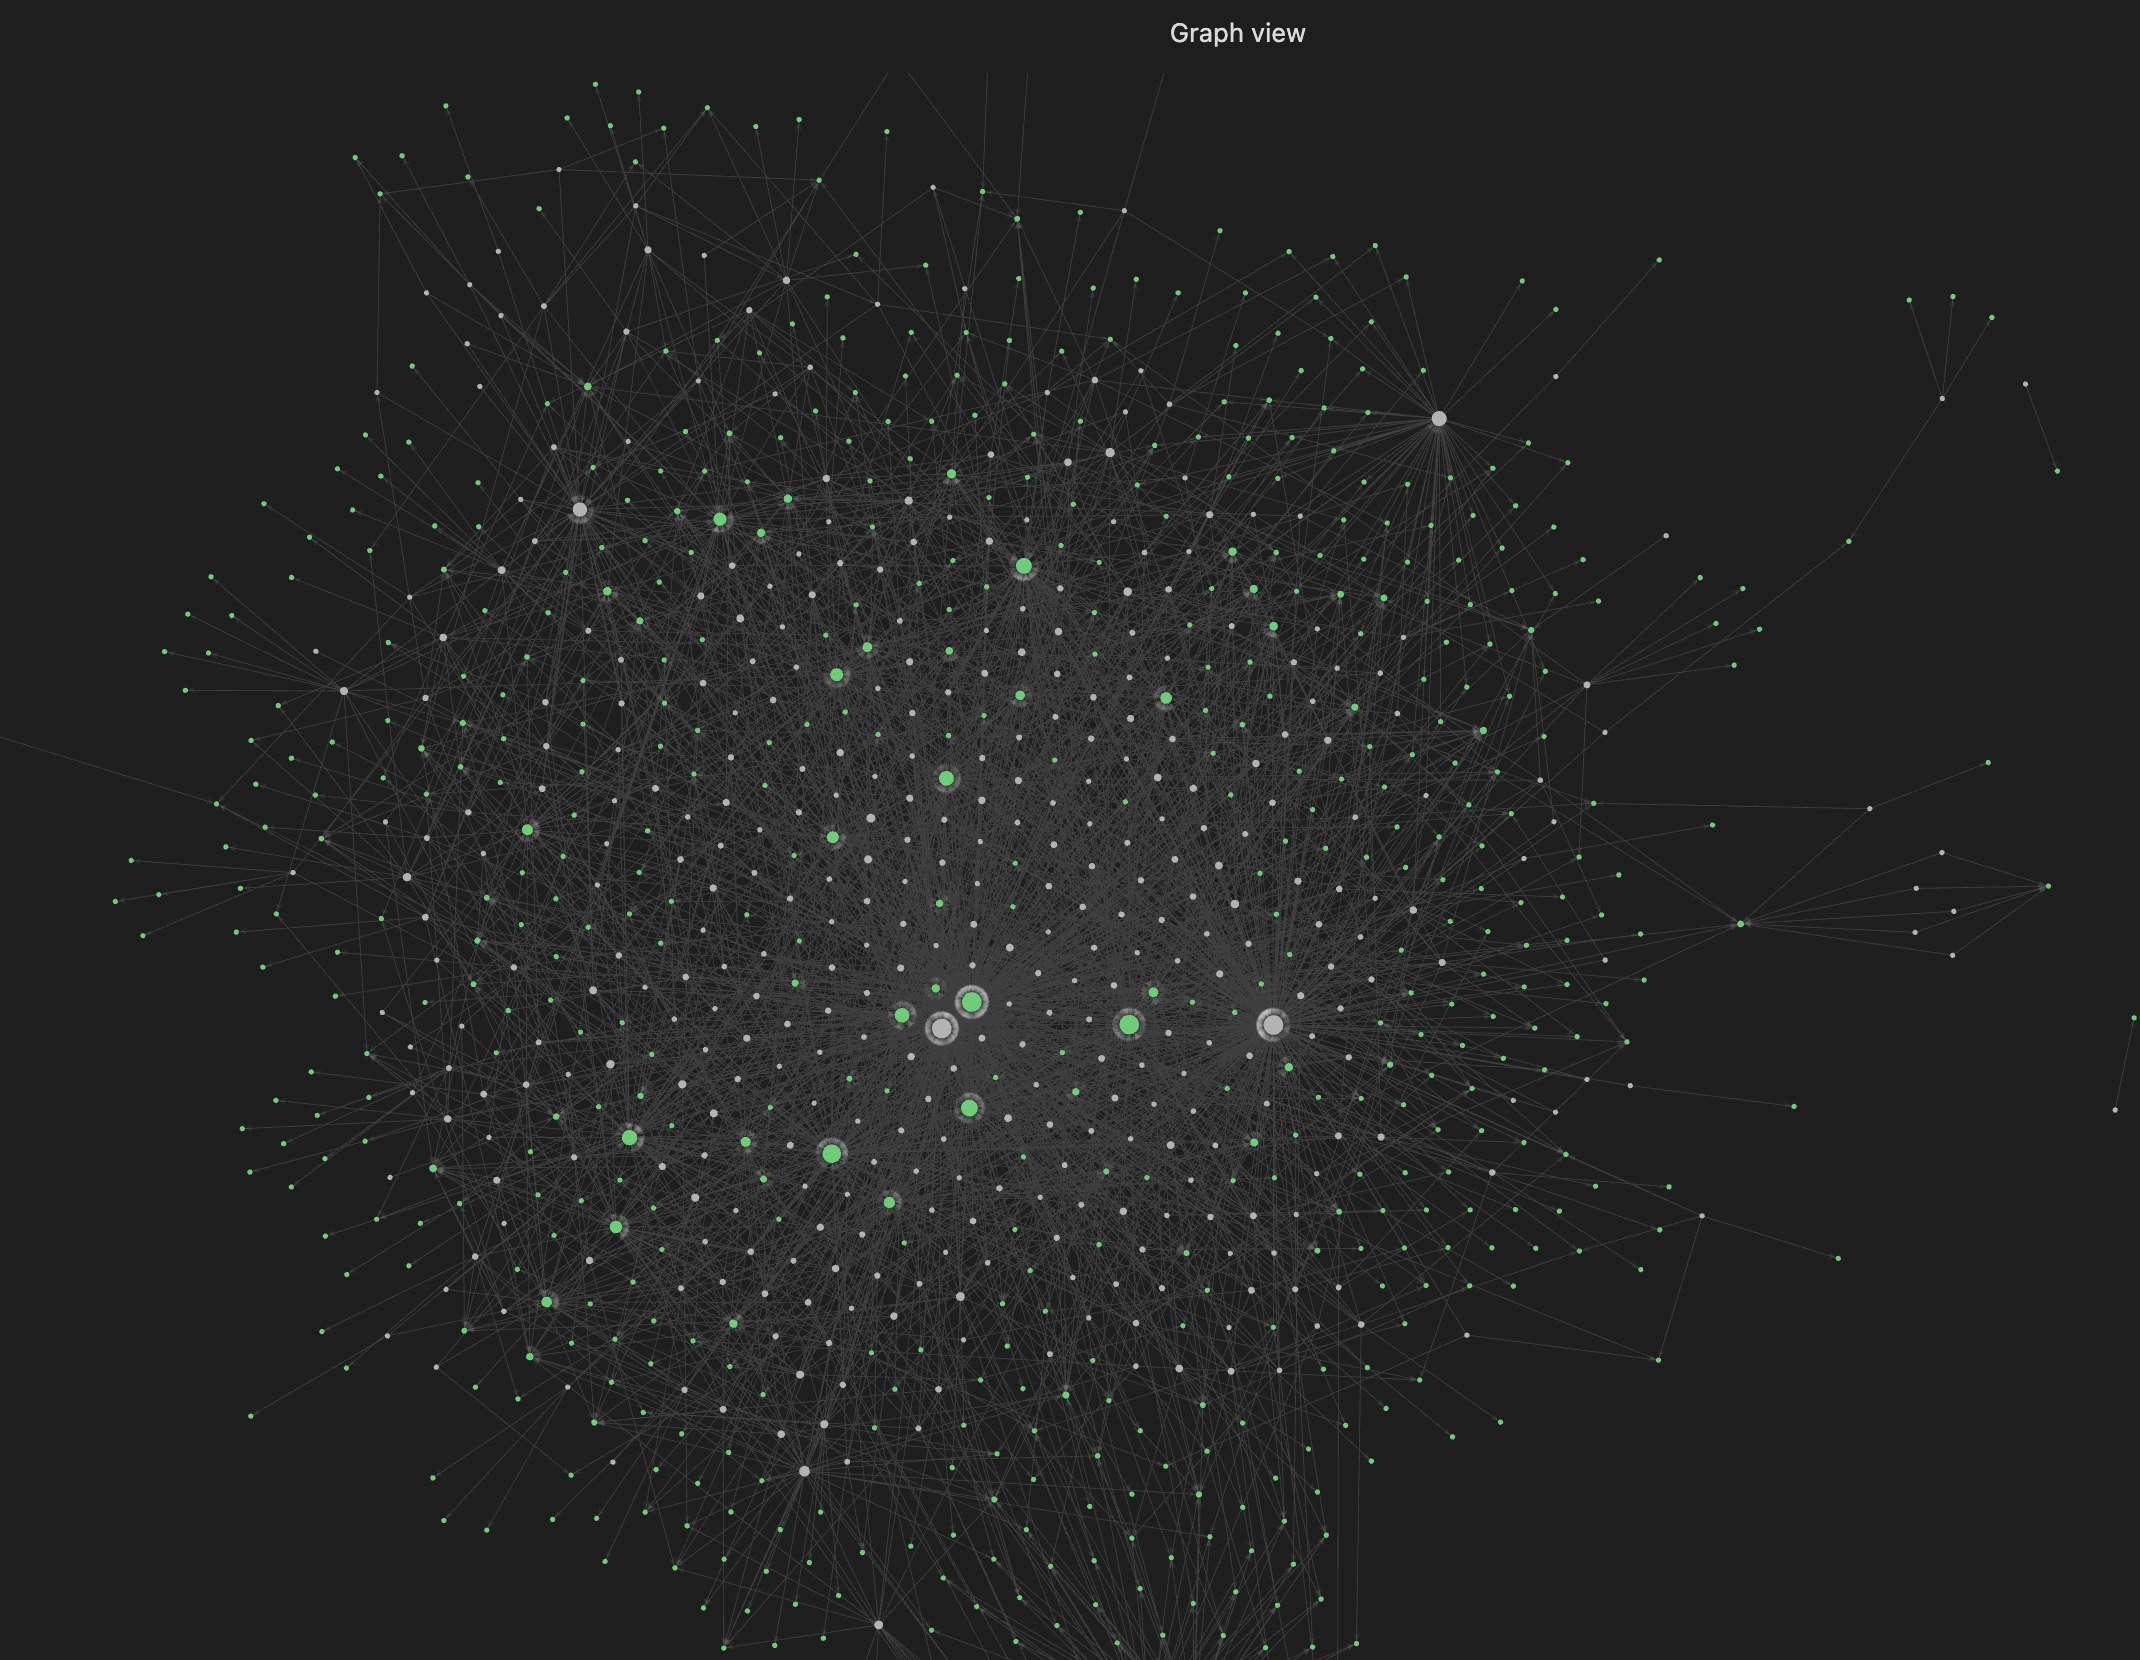
\includegraphics{assets/u3/graph1.png}

\end{figure}%

You can click any of the tags in Obsidian to see highlighted connections
and search results for that tag, allowing you to go directly to notes of
interest.

\begin{figure}

\caption{\label{fig-graph3}Screenshot, Graph View in Obsidian With Tag
Expanded to Show Additional Information}

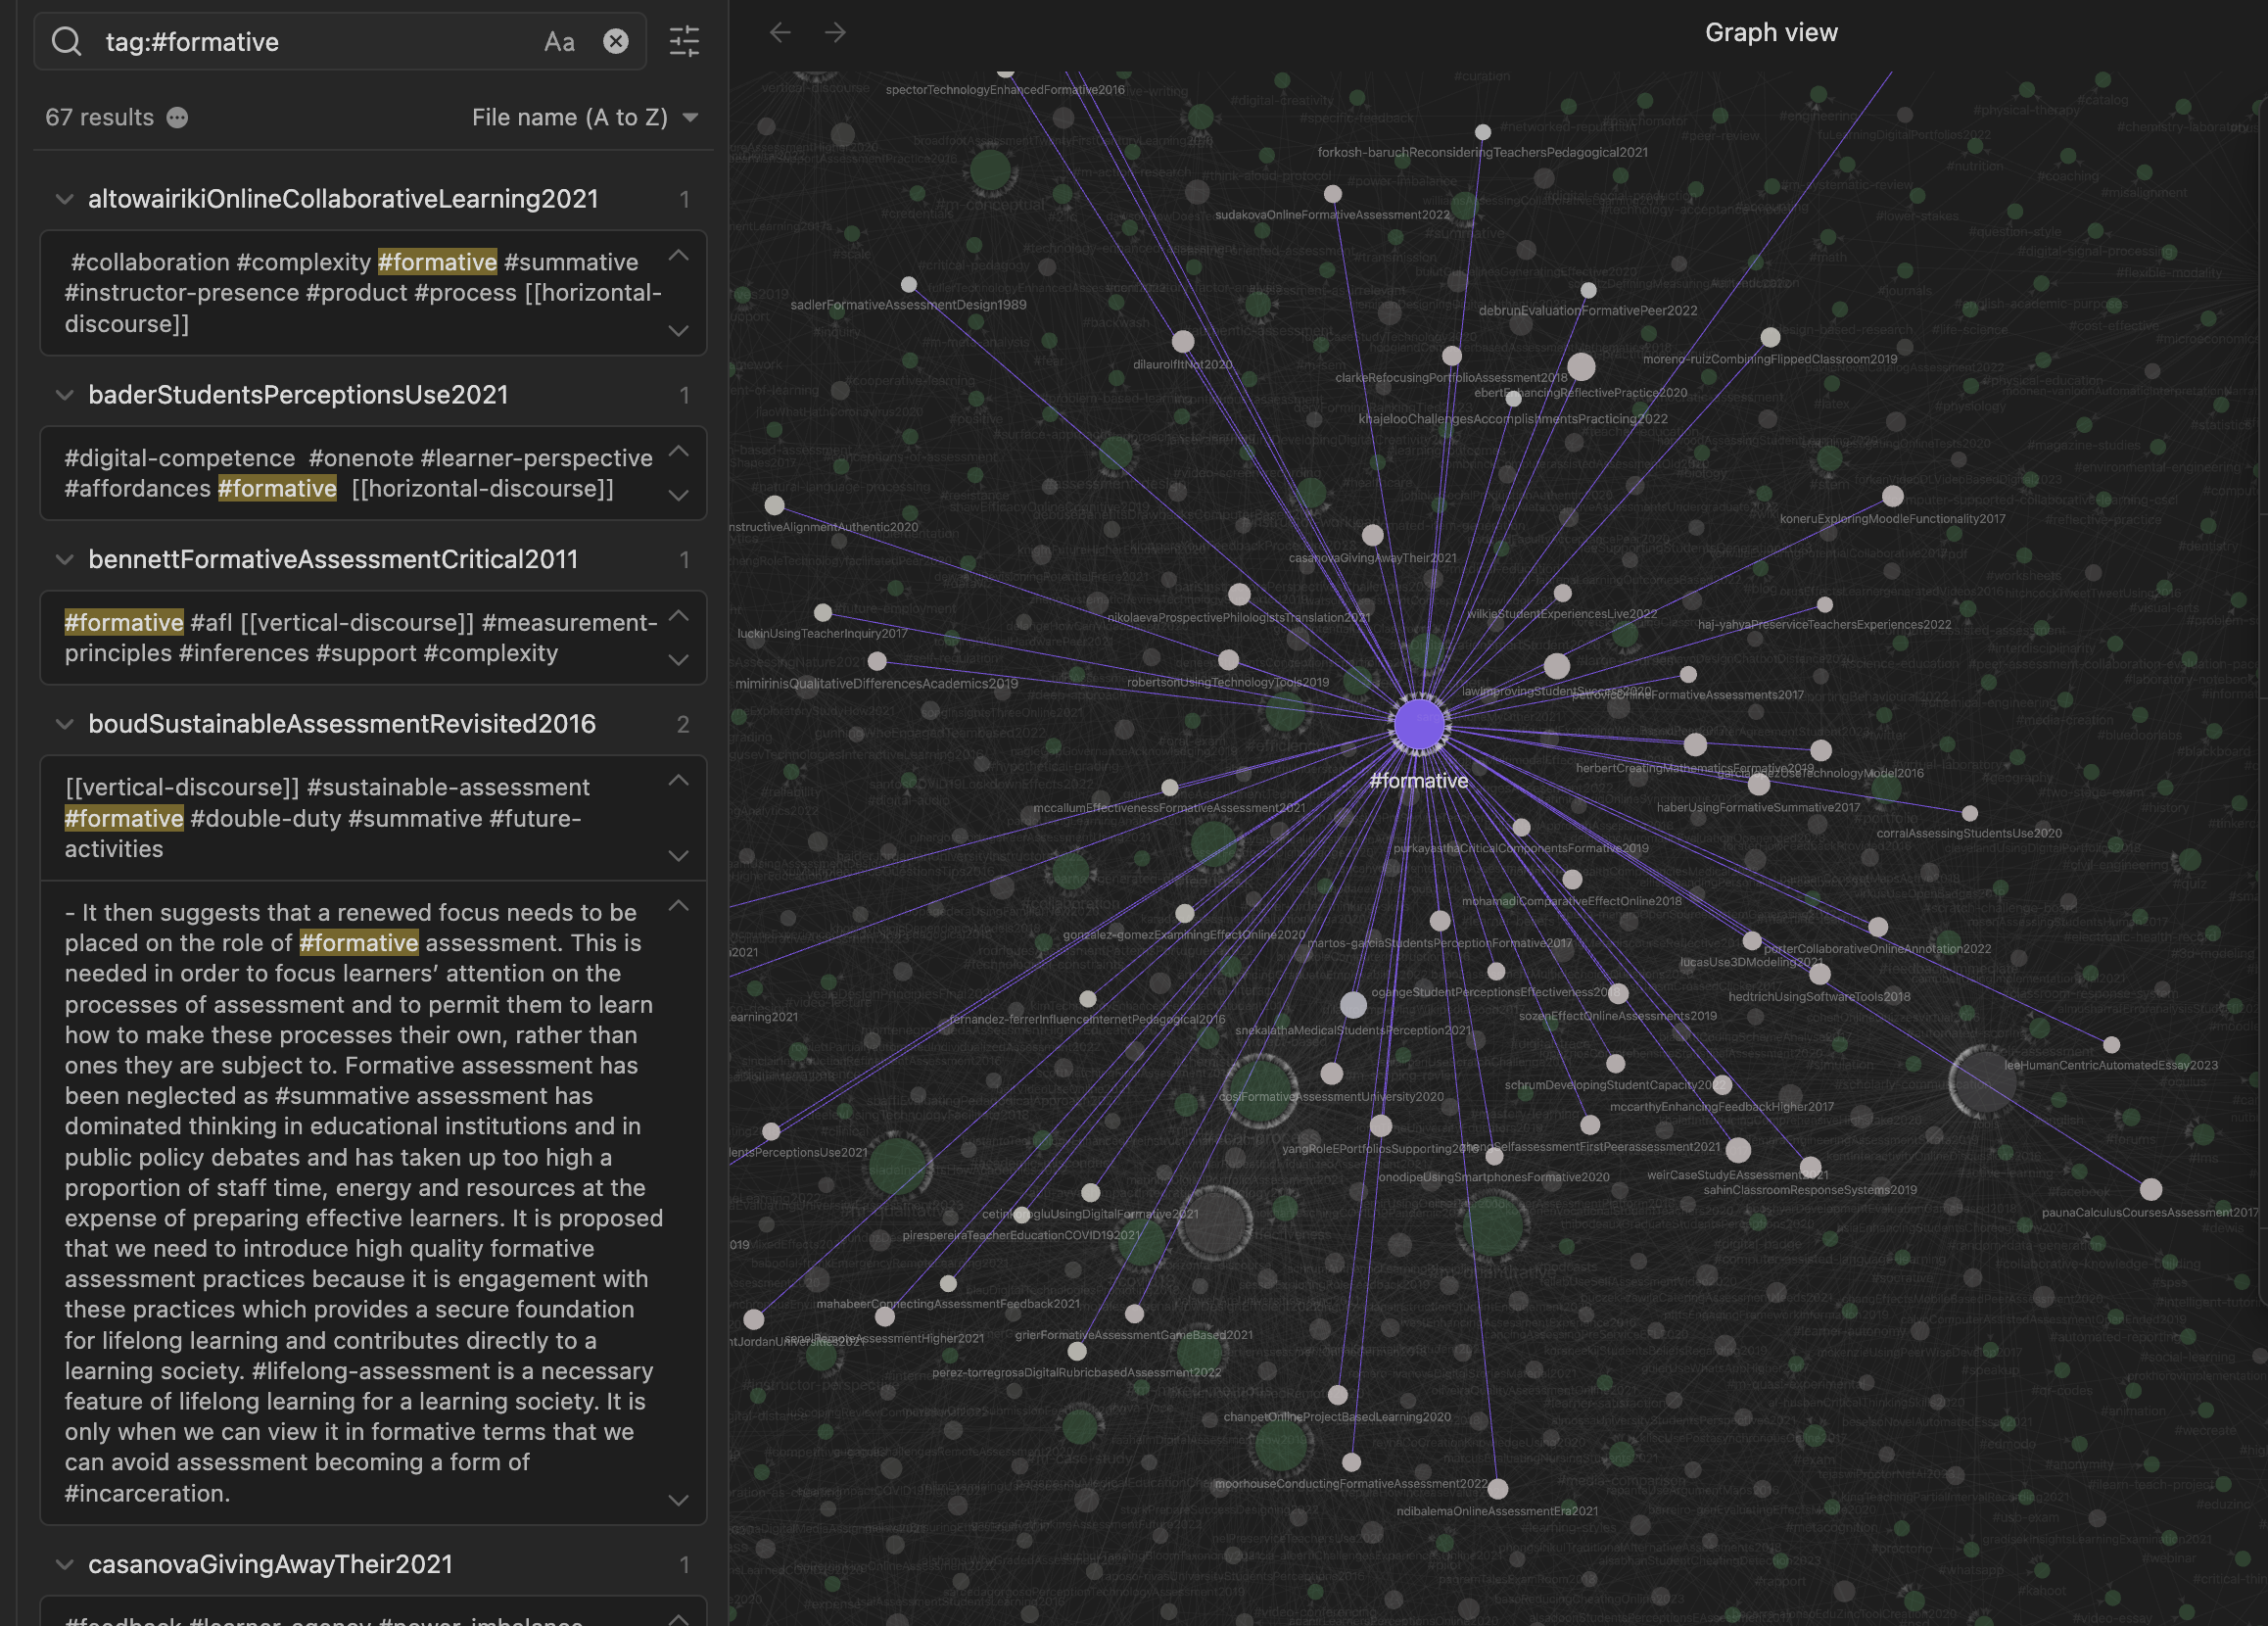
\includegraphics{assets/u3/graph3.png}

\end{figure}%

Using links and tags together you can build a very powerful and easily
searchable vault of all the ideas in your courses. This can be
incredibly valuable when it is time to write a paper or prepare for an
exam---you can have all your notes easily accessible rather than having
to search through pages and pages of handwritten notes.

\subsection{Activity: Tag, Link, Connect, and
Reflect}\label{activity-tag-link-connect-and-reflect}

\begin{tcolorbox}[enhanced jigsaw, toprule=.15mm, colback=white, colframe=quarto-callout-note-color-frame, bottomtitle=1mm, leftrule=.75mm, coltitle=black, titlerule=0mm, rightrule=.15mm, colbacktitle=quarto-callout-note-color!10!white, left=2mm, title={Learning Activity}, opacitybacktitle=0.6, opacityback=0, breakable, toptitle=1mm, arc=.35mm, bottomrule=.15mm]

\begin{itemize}
\tightlist
\item
  \textbf{Tag}: Follow the directions above to add tags to your notes in
  Obsidian. Again, spend some time on this. The more you practice, the
  easier the process will be. More than that, as you continue to use
  tags and links, you will be able to experience the advantages of
  connecting your ideas using this method.
\item
  \textbf{Write}: Add to your Reflective Journal your thoughts and
  experience on using tags. What were your struggles or ``ah-ha''
  moments? What questions do you have? Remember to reach out for support
  on the Learning Hub in Discourse.
\end{itemize}

\end{tcolorbox}

\section{Sense-making Through Concept
Maps}\label{sense-making-through-concept-maps}

As you saw at the beginning of this unit, sense-making is the
\textbf{work} of learning. There is no way around the work of learning
because learning is work. It takes time and cognitive effort. As much as
we wish to be able to ``learn'' like Neo in \emph{The Matrix}, we can't
(see a favourite scene in a movie, below; and it's not just because
Keanu Reeves is the GOAT 🐐).

\begin{itemize}
\tightlist
\item
  \textbf{Watch}: \href{https://www.youtube.com/watch?v=0YhJxJZOWBw}{The
  Matrix - `I Know Kung Fu'} (2019)
\end{itemize}

\url{https://www.youtube-nocookie.com/embed/0YhJxJZOWBw}

Tags and links in Obsidian can be visualized using graph view, but as
this is an algorithmically generated map of the connections between
ideas and files in your vault, there is little you can do to customize
it. Fortunately, Obsidian also features a tool called the Canvas, which
is a blank space that you can use to manually connect ideas in a visual
format, allowing you to see connections and relationships that make
sense to you. The following video is a brief explanation of how to use
the Canvas in Obsidian.

\subsection{Activity: Obsidian Concept
Map}\label{activity-obsidian-concept-map}

\begin{itemize}
\tightlist
\item
  \textbf{Watch}:
  \href{https://www.youtube.com/watch?v=eHI-Szjpafk}{\emph{Mind Mapping
  in Obsidian Canvas}} (2023). As you watch, follow the directions and
  to create a concept map in Obsidian. You will use this in the next
  activity.
\end{itemize}

\url{https://www.youtube-nocookie.com/embed/eHI-Szjpafk}

\subsection{Activity: Open Source Video and Audio
Lectures}\label{activity-open-source-video-and-audio-lectures}

\begin{tcolorbox}[enhanced jigsaw, toprule=.15mm, colback=white, colframe=quarto-callout-note-color-frame, bottomtitle=1mm, leftrule=.75mm, coltitle=black, titlerule=0mm, rightrule=.15mm, colbacktitle=quarto-callout-note-color!10!white, left=2mm, title={Learning Activity}, opacitybacktitle=0.6, opacityback=0, breakable, toptitle=1mm, arc=.35mm, bottomrule=.15mm]

\begin{itemize}
\tightlist
\item
  \textbf{Search}: Search for a video or audio lecture on a topic of
  interest. Use your advanced search skills or browse the following
  sites to find a suitable recording aligned with your interests:

  \begin{itemize}
  \tightlist
  \item
    \href{https://www.openculture.com/freeonlinecourses}{\emph{Open
    Culture}} (2024). Over 30,000 hours of free audio and video lectures
  \item
    \href{https://oyc.yale.edu/}{\emph{Open Yale Courses}} (2024). Free
    and open access to a selection of introductory courses including
    video lectures from Yale University(2024).
  \item
    \href{https://extension.harvard.edu/online-learning/}{\emph{Harvard
    Online Courses}}(2024) Series of video lectures from Harvard
    University.
  \item
    \href{https://ocw.mit.edu/search/?f=Lecture\%20Videos&f=Lecture\%20Audio&s=department_course_numbers.sort_coursenum}{\emph{MIT
    OpenCourseWare}}(2024) Series of audio and video lectures from
    Massachusetts Institute of Technology
  \item
    \href{https://www.ted.com/}{\emph{Tedx Talks}} (2024). Extensive
    database of video presentations in the form of short, powerful talks
    (see also list of topics)
  \end{itemize}
\item
  \textbf{Write}: Using Obsidian, record your notes from the lecture.

  \begin{itemize}
  \tightlist
  \item
    the first line is used for the title of the note
  \item
    remember to include a link to the source of the information
  \item
    use tags and links to connect your ideas
  \end{itemize}
\end{itemize}

\end{tcolorbox}

\section{Reading and Note Taking}\label{reading-and-note-taking}

Next, let's focus on reading and note taking. In this section, you will
demonstrate your note taking skills based on reading an academic
publication. You will also have the opportunity to practice using the
Markdown markup language. Semantic markup is an important digital skill
that separates formatting (e.g., headings, bold, italics, lists) from
content, using designated characters without the use of rich text
editors. This provides the capability to use plain text files that can
be converted to formatted text online. Markdown is one of many such
markup protocols and is used here to demonstrate the principles of
semantic markup.

\subsection{Activity: Reading and Note
Taking}\label{activity-reading-and-note-taking}

\begin{tcolorbox}[enhanced jigsaw, toprule=.15mm, colback=white, colframe=quarto-callout-note-color-frame, bottomtitle=1mm, leftrule=.75mm, coltitle=black, titlerule=0mm, rightrule=.15mm, colbacktitle=quarto-callout-note-color!10!white, left=2mm, title={Learning Activity}, opacitybacktitle=0.6, opacityback=0, breakable, toptitle=1mm, arc=.35mm, bottomrule=.15mm]

\begin{itemize}
\tightlist
\item
  \textbf{Read} the following articles and take notes in Obsidian. Try
  using Markdown to format your text.

  \begin{itemize}
  \tightlist
  \item
    \href{https://www.student.unsw.edu.au/effective-reading-and-note-taking}{\emph{Effective
    Reading and Note-Taking}} (n.d.)
  \item
    \href{https://www.student.unsw.edu.au/reading-understanding}{\emph{Reading
    for Understanding: The SQW3R Method}} (2024)
  \item
    \href{https://www.science.org/content/article/how-seriously-read-scientific-paper}{\emph{How
    to (Seriously) Read a Scientific Paper}} (2016)
  \item
    \emph{Using Markdown in Obsidian} (n.d.)
  \end{itemize}
\end{itemize}

\end{tcolorbox}

\subsection{Activity: Writing a Summary of Your
Readings}\label{activity-writing-a-summary-of-your-readings}

\begin{tcolorbox}[enhanced jigsaw, toprule=.15mm, colback=white, colframe=quarto-callout-note-color-frame, bottomtitle=1mm, leftrule=.75mm, coltitle=black, titlerule=0mm, rightrule=.15mm, colbacktitle=quarto-callout-note-color!10!white, left=2mm, title={Learning Activity}, opacitybacktitle=0.6, opacityback=0, breakable, toptitle=1mm, arc=.35mm, bottomrule=.15mm]

In this activity you will read an academic article and write a summary
using Obsidian and Zotero.

\begin{itemize}
\tightlist
\item
  \textbf{Read}:

  \begin{itemize}
  \tightlist
  \item
    First, search for a peer reviewed journal article in support of a
    research topic of interest
  \item
    Remember to add the source to your citation management tool, Zotero
  \end{itemize}
\item
  \textbf{Write}:

  \begin{itemize}
  \tightlist
  \item
    Prepare a summary of the journal article based on this example
  \item
    Use the Markdown formatting in Obsidian. Your summary must at a
    minimum demonstrate the following text formats:

    \begin{itemize}
    \tightlist
    \item
      headings and subheadings
    \item
      bold and italics
    \item
      numbered or unordered list
    \item
      labelled link
    \item
      horizontal rule
    \item
      block quote for one or more citations from the article
    \end{itemize}
  \item
    Copy your summary prepared in Obsidian and paste this text summary
    into Zotero using the notes feature so that you have a copy for your
    personal library as backup.
  \end{itemize}
\end{itemize}

Reflect on your progress in practicing these digital skills. Share your
thoughts in your journal and/or in Discourse.

\end{tcolorbox}

\section{Digital Tools To Support
Learning}\label{digital-tools-to-support-learning}

So far in this course you have had opportunities to explore a number of
learning tools, including \href{https://obsidian.md}{Obsidian},
\href{https://www.zotero.org/}{Zotero}, and
\href{https://www.litmaps.com/}{LitMaps}.

We anticipate these tools will help you think critically, collaborate,
and ultimately succeed in your studies.

There is a plethora of other learning tools out there. We encourage you
to explore various apps and evaluate them based on criteria you value
(effectiveness, privacy, cost, data ownership, accessibility, and so
on).

\subsection{Activity: Tools for Learning in
University}\label{activity-tools-for-learning-in-university}

\begin{tcolorbox}[enhanced jigsaw, toprule=.15mm, colback=white, colframe=quarto-callout-note-color-frame, bottomtitle=1mm, leftrule=.75mm, coltitle=black, titlerule=0mm, rightrule=.15mm, colbacktitle=quarto-callout-note-color!10!white, left=2mm, title={Learning Activity}, opacitybacktitle=0.6, opacityback=0, breakable, toptitle=1mm, arc=.35mm, bottomrule=.15mm]

\begin{itemize}
\tightlist
\item
  \textbf{Explore}: Search for the following apps or websites using the
  key words listed below. Try adding ``top,'' ``best,'' ``free,''
  ``university,'' or ``students'' and see how that changes your search
  results.

  \begin{itemize}
  \tightlist
  \item
    note taking apps
  \item
    annotate web resources
  \item
    collaborative tools
  \item
    project management tools
  \item
    graphic organizers
  \item
    study tools
  \item
    focus tools
  \item
    research tools
  \item
    writing tools
  \end{itemize}
\item
  \textbf{Share}: In Discourse, share some tools that you've used or
  that you plan to use to help in your studies.
\end{itemize}

\end{tcolorbox}

\section*{Summary}\label{summary-2}
\addcontentsline{toc}{section}{Summary}

\markright{Summary}

As we conclude our unit, reflect on your learning. Throughout this unit,
you've acquired a multifaceted skill set that empowers you to harness
the potential of technology in synthesizing and organizing knowledge.
From understanding the intricate dance of hyperlinks and tags, to
mastering the art of digital note taking, you've explored tools and
strategies that redefine how we connect ideas in the digital age.

Concept maps have become your canvas, allowing you to visually
articulate complex relationships and hierarchies with precision and
clarity. The curated digital tools we've explored are now at your
disposal, enhancing your learning experience and catering to your unique
preferences. Remember, this unit isn't just about understanding
concepts; it's about applying these newfound skills in real world
scenarios.

As you move forward, carry this digital toolkit with you, leveraging
technology as a powerful ally in your ongoing pursuit of knowledge. Your
ability to connect ideas seamlessly through hyperlinks, tags, note
taking, and concept maps positions you as a dynamic learner in an ever
evolving educational landscape. The skills you've honed here are not
just for this course but are lifelong assets that will continue to
enrich your learning journey.

\begin{tcolorbox}[enhanced jigsaw, toprule=.15mm, colback=white, colframe=quarto-callout-note-color-frame, bottomtitle=1mm, leftrule=.75mm, coltitle=black, titlerule=0mm, rightrule=.15mm, colbacktitle=quarto-callout-note-color!10!white, left=2mm, title={Checking Your Learning}, opacitybacktitle=0.6, opacityback=0, breakable, toptitle=1mm, arc=.35mm, bottomrule=.15mm]

Before you move on to the next unit check that you are able to:

\begin{itemize}
\tightlist
\item
  Build and customize technology integrated workflows to enhance and
  enrich your learning journey
\item
  Practice evaluative judgment to document your process of learning in
  complex domains of knowledge
\item
  Evaluate digital tools, platforms, and interactions based on ethical
  principles
\end{itemize}

\end{tcolorbox}

\bookmarksetup{startatroot}

\chapter{Building Your Online
Presence}\label{building-your-online-presence}

\section*{Overview}\label{overview-3}
\addcontentsline{toc}{section}{Overview}

\markright{Overview}

Welcome to Unit 4! In previous units, you've been introduced to the
world of digital literacies and learned how to utilize various tools for
organizing and connecting ideas. You have started to build a workflow to
help you learn more effectively and have applied the critical skill of
metacognition to explain your process for learning.

Now, let's dive into the next phase of our learning journey.

In the second half of the course, you will continue to build your
digital skills and apply critical thinking to document your learning
process. Our focus will shift from creating a personal collection of
ideas to presenting your learning in a more open platform. It's
important to emphasize that \emph{you} will decide how public you want
this to be. We'll also explore the significance of knowledge sharing and
examine user-friendly methods to do so while maintaining control over
your work and addressing privacy concerns. As you begin this unit, take
a moment to reflect on your personal and academic goals as they relate
to digital literacy. Consider which digital tools you'd like to explore,
and reflect on how your online contributions can not only benefit your
own growth but also contribute positively to others.

\subsection*{Topics}\label{topics-3}
\addcontentsline{toc}{subsection}{Topics}

This unit is divided into the following topics:

\begin{enumerate}
\def\labelenumi{\arabic{enumi}.}
\tightlist
\item
  Personal learning environments
\item
  Building a learning blog
\item
  My digital footprint
\item
  Evaluating digital tools
\end{enumerate}

\subsection*{Learning Outcomes}\label{learning-outcomes-2}
\addcontentsline{toc}{subsection}{Learning Outcomes}

When you have completed this unit you will be able to:

\begin{itemize}
\tightlist
\item
  Create a personalized narrative to document and express your learning
  process
\item
  Examine your digital footprint and develop a positive digital online
  identity
\item
  Evaluate digital tools, platforms, and interactions based on ethical
  principles
\item
  Critically evaluate the affordances and restraints of digital tools
  and platforms
\item
  Identify the digital skills needed in your field of study
\item
  Describe how to protect yourself and other students and colleagues to
  stay safe in the digital environment
\item
  Practice evaluative judgment to document your process of learning in
  complex domains of knowledge
\end{itemize}

\subsection*{Activity Checklist}\label{activity-checklist-3}
\addcontentsline{toc}{subsection}{Activity Checklist}

Here is a checklist of learning activities you will benefit from in
completing this unit. You may find it useful for planning your work.

\begin{tcolorbox}[enhanced jigsaw, toprule=.15mm, colback=white, colframe=quarto-callout-note-color-frame, bottomtitle=1mm, leftrule=.75mm, coltitle=black, titlerule=0mm, rightrule=.15mm, colbacktitle=quarto-callout-note-color!10!white, left=2mm, title={Learning Activity}, opacitybacktitle=0.6, opacityback=0, breakable, toptitle=1mm, arc=.35mm, bottomrule=.15mm]

\textbf{Learning Activities}

\begin{itemize}
\tightlist
\item
  Reflect on your personal learning environment (PLE) as you engage with
  the resources on PLEs
\item
  Create a new blog on WordPress and personalize your blog site
\item
  Conduct a digital footprint audit to assess your online presence
\item
  Document and share your learning experience by publishing a blog entry
\item
  Evaluate a digital tool, considering the ethical implications
\end{itemize}

\begin{tcolorbox}[enhanced jigsaw, toprule=.15mm, colback=white, colframe=quarto-callout-note-color-frame, arc=.35mm, opacityback=0, breakable, rightrule=.15mm, bottomrule=.15mm, leftrule=.75mm, left=2mm]

\emph{Note: Working through course activities will help you to meet the
learning outcomes and successfully complete your assessments.}

\end{tcolorbox}

\end{tcolorbox}

\begin{tcolorbox}[enhanced jigsaw, toprule=.15mm, colback=white, colframe=quarto-callout-note-color-frame, arc=.35mm, opacityback=0, breakable, rightrule=.15mm, bottomrule=.15mm, leftrule=.75mm, left=2mm]

\textbf{Assessment}

\begin{itemize}
\tightlist
\item
  See the Assessment section in Moodle for assignment details and due
  dates.
\end{itemize}

\end{tcolorbox}

\subsection*{Resources}\label{resources-3}
\addcontentsline{toc}{subsection}{Resources}

\begin{itemize}
\tightlist
\item
  All resources will be provided online in the unit.
\end{itemize}

\begin{tcolorbox}[enhanced jigsaw, toprule=.15mm, colback=white, colframe=quarto-callout-note-color-frame, arc=.35mm, opacityback=0, breakable, rightrule=.15mm, bottomrule=.15mm, leftrule=.75mm, left=2mm]
\begin{minipage}[t]{5.5mm}
\textcolor{quarto-callout-note-color}{\faInfo}
\end{minipage}%
\begin{minipage}[t]{\textwidth - 5.5mm}

\textbf{\emph{Resource Reminders}}

\begin{itemize}
\tightlist
\item
  Remember to continuously add resources to your Zotero library that
  align with your learning goals
\item
  Utilize your community---peers, coworkers, and online communities---as
  valuable resources! Stay engaged to seek assistance and exchange
  helpful resources and insights
\end{itemize}

\end{minipage}%
\end{tcolorbox}

\section{Personal Learning
Environments}\label{personal-learning-environments}

This unit aims to guide you in creating your Learning Blog, the central
component of your personal learning environment (PLE). Blog posts serve
as reflections on your learning journey and facilitate networking with
peers. Your blog also provides your instructor with valuable insights
into your course engagement and learning process. Ultimately, the goal
of a PLE is to put the learner at the centre of the online learning
environment.

\textbf{So What is a Personal Learning Environment?}

Personal Learning Environments {[}are{]} systems that help learners take
control of and manage their own learning. This includes providing
support for learners to set their own learning goals, manage their
learning; managing both content and process, communicate with others in
the process of learning, and thereby achieve learning goals. A PLE may
be composed of one or more sub-systems: As such it may be a desktop
application, or composed of one or more web-based services. (van
Harmelen, 2007, as cited in Edutech Wiki, 2014, Definitions, para. 2)

Which aspects of the two definitions do you find most meaningful? How do
you structure your daily interactions and manage the flow of
information? In what ways do you communicate your learning experiences
to others? Lastly, what specific goals are you aiming to accomplish
through your learning journey?

\subsection{Activity: What Is a PLE?}\label{activity-what-is-a-ple}

\begin{tcolorbox}[enhanced jigsaw, toprule=.15mm, colback=white, colframe=quarto-callout-note-color-frame, bottomtitle=1mm, leftrule=.75mm, coltitle=black, titlerule=0mm, rightrule=.15mm, colbacktitle=quarto-callout-note-color!10!white, left=2mm, title={Learning Activity}, opacitybacktitle=0.6, opacityback=0, breakable, toptitle=1mm, arc=.35mm, bottomrule=.15mm]

\begin{itemize}
\item
  \textbf{Read}: Before you start building your PLE, read the following
  article: ``\emph{7 Things you Should Know About Personal Learning
  Environments.} After reading the article, consider the following:
\item
  \textbf{Questions to Consider:}

  \begin{itemize}
  \tightlist
  \item
    How do PLEs promote authentic, student-centred learning?
  \item
    What are the benefits of a PLE? How would it benefit you?
  \item
    What tools do you currently use as part of your learning
    environment?
  \end{itemize}
\item
  \textbf{Watch}: Finally, consider the approach taken at TWU as it
  supports inquiry-rich learning. As you watch the short video below,
  think about how you could use your PLE to enrich your learning at TWU.
\end{itemize}

\href{https://www.youtube.com/watch?v=SCa9Nt3X1vU}{Watch: * Inquiry-Rich
Learning*}(2018)

\url{https://www.youtube-nocookie.com/embed/SCa9Nt3X1vU}

\end{tcolorbox}

\subsection{Activity: What Is Your
Ple?}\label{activity-what-is-your-ple}

\begin{tcolorbox}[enhanced jigsaw, toprule=.15mm, colback=white, colframe=quarto-callout-note-color-frame, bottomtitle=1mm, leftrule=.75mm, coltitle=black, titlerule=0mm, rightrule=.15mm, colbacktitle=quarto-callout-note-color!10!white, left=2mm, title={Learning Activity}, opacitybacktitle=0.6, opacityback=0, breakable, toptitle=1mm, arc=.35mm, bottomrule=.15mm]

\begin{itemize}
\item
  \textbf{Write}: Take a couple of minutes to brainstorm the tools,
  services, and communities that you use to pursue your educational
  goals. Use your notetaking tool (e.g., Obsidian) to create a list of
  these.
\item
  \textbf{Create}: Next, create a graphic organizer to visualize your
  PLE. You can use Obsidian, or see
  \href{https://www.techlearning.com/news/best-graphic-organizers-for-education}{\emph{Best
  Graphic Organizers for Education}} (2023) for other free options.
\end{itemize}

\begin{tcolorbox}[enhanced jigsaw, toprule=.15mm, colback=white, colframe=quarto-callout-note-color-frame, arc=.35mm, opacityback=0, breakable, rightrule=.15mm, bottomrule=.15mm, leftrule=.75mm, left=2mm]

Note that you completed a Visitor and Resident Diagram Activity in Unit
1. Feel free to use that graphic organizer and add other tools you use
for learning, or that you have been introduced to in this course.

You will be encouraged to post your PLE graphic on your blog \ldots{}
which you will start in the next activity!

\end{tcolorbox}

\end{tcolorbox}

\section{Building a Learning Blog}\label{building-a-learning-blog}

In the next activity, you will gain firsthand experience in using blog
technology for publishing your own website. You will ``declare''
yourself online using your PLE as an alternative to posting an
introduction in a closed course forum typically used in a conventional
online course. Note that TWU online courses often use Moodle Discussion
Forums to facilitate conversations. By using a platform such as
WordPress you can retain the contents of your posts as well as the
comments of your peers. In a learning management system (LMS) such as
Moodle you may lose access to what you have posted in discussions, and
more importantly, conversations with your peers. As you create your
personal blog in WordPress (or your own selective blog site), you
control your data and who can see it.

You will retain control of your data and learning outputs generated
during this online course, even after the course is completed. You get
to choose:

The blog service you would like to use, although \textbf{we recommend
WordPress as it is supported by TWU}Whether to accept comments on your
blog from your peersWhether to register your blog for the aggregated
course feed so that any posts tagged with the course code (LDRS101) will
be harvested for the feedA key teaching philosophy of this course is to
embed the acquisition of new digital literacies into your learning
journey. Knowledge of how to use the internet and social media
technologies will better prepare you for life in a digital world. If
this is your first time blogging, you should spend time setting up your
personal digital learning environment. Please remember that your
learning blog and the social media technologies you use on this course
are public, and that you take full responsibility for anything you
publish. Do not disclose any confidential information and respect the
privacy of others. In short, don't say anything that you would not want
to read on the internet.

\subsection{Activity: Setting up Your Learning
Blog}\label{activity-setting-up-your-learning-blog}

\begin{tcolorbox}[enhanced jigsaw, toprule=.15mm, colback=white, colframe=quarto-callout-note-color-frame, bottomtitle=1mm, leftrule=.75mm, coltitle=black, titlerule=0mm, rightrule=.15mm, colbacktitle=quarto-callout-note-color!10!white, left=2mm, title={Learning Activity}, opacitybacktitle=0.6, opacityback=0, breakable, toptitle=1mm, arc=.35mm, bottomrule=.15mm]

As this is a course focusing on digital literacies, you are asked to
establish a Learning Blog, which will improve your skills and enable you
to network with your peers. We recommend using WordPress, as it is
supported by TWU. WordPress is an open source website builder and is one
of the most popular systems available because of its versatility. If you
already have your own website or you have previous experience using
WordPress, you may set up your blog on it and skip the set-up steps
described below, but you still need to complete the learning activities.

We are here to help you create your site, so do not hesitate to ask for
technical support. There are a number of resources below, but if you get
stuck, please reach out on Discourse, or email elearning@twu.ca

To get started on creating your site we suggest the following steps:

\begin{itemize}
\tightlist
\item
  \textbf{Sign up to create a website}

  \begin{itemize}
  \tightlist
  \item
    Go to \href{https://create.twu.ca/}{\textbf{create.twu.ca}} to sign
    up for your free WordPress site. \emph{Please read all the prompts
    and instructions carefully!} Be sure to read the Privacy Statement
    carefully before clicking ``I Agree.'' The information provided
    gives you excellent guidance regarding digital citizenship, privacy,
    and how to build a professional digital persona.
  \item
    You will be prompted to \textbf{create a domain name}, which is your
    website's address on the internet. Often this is referred to as a
    URL (Uniform Resource Locator). This is what your users will type in
    their browsers to reach your site. Make sure that you choose a
    domain name that is related to you, easy to pronounce and spell, and
    easy to remember. Once you have done that, we suggest you write all
    this information somewhere you can access it easily---just in case.
  \item
    You will also be asked to \textbf{select a theme} for your website.
    You are free to choose any template you wish. TWU Spark, TWU Hope,
    and TWU Spartans portfolios are simple to set up and provide easy
    navigation.
  \item
    When you choose your theme, your new site will come with a simple
    menu and instructions for portfolio and website creation.
  \item
    Once you have activated your site (look for a notification in your
    TWU email) you are ready to create.
  \end{itemize}
\item
  \textbf{Explore your dashboard}

  \begin{itemize}
  \tightlist
  \item
    The dashboard is the initial area you see when you log in to TWU
    Create. It's the centre for your site management and where you
    create content. From the Dashboard you can navigate to content,
    settings, themes, plugins, and more.
  \item
    When logged in to TWU Create, you will always have access to an
    \textbf{admin menu} visible on your sites. From the menu item that
    is the name of the blog (second from left), you can find the link to
    the dashboard. While in the dashboard, the same menu can be used to
    return to the front view of your site.
  \item
    Determine the difference between the dashboard used for editing and
    the published view of your blog. (It is important to know the
    difference because when you register your blog for the course feed,
    you must use the URL for the public view of your blog).
  \end{itemize}
\end{itemize}

\emph{Progress check:} - Do you know how to open the published (public
view) of your blog in a new window? - Have you added a browser bookmark
to your dashboard and the public version of your blog?

\textbf{Help Tips:} When you are in the site administration area of your
site, you can get tips on what you are doing by clicking the ``Help''
menu on the top righthand corner. Click ``Help'' and read through the
Overview describing the elements of the dashboard.

\begin{itemize}
\tightlist
\item
  \textbf{Review your settings:} Review and customize your blog settings
  from the dashboard according to your preferences.

  \begin{itemize}
  \tightlist
  \item
    \textbf{Enable categories and tags:} We recommend that you enable
    \textbf{categories} and \textbf{tags} on your blog.
    \textbf{Categories} are best used for broad groupings of topics. For
    example, if you're creating a site that reviews pop culture you
    might use categories such as books, film, and TV. \textbf{Tags} are
    more specific keywords that you want to use to associate related
    content. For example, if you were creating a site that reviews pop
    culture you might want to use tags such as science fiction, horror,
    and action adventure.You can combine the two! For our review site
    example, you might be reviewing a romantic comedy. You can assign
    the broader category ``film'' to the post, then give it some more
    specific tags such as romantic comedy, or even use the name of the
    actors and director as tags. People who view that post could use the
    tags to find related posts around that topic.
  \item
    \textbf{Set up comments settings (optional):} WordPress comes with a
    built-in comment system allowing your users to leave comments on
    your posts. This comment system is great for user engagement, but it
    can also be targeted by spammers as well. If you don't want comments
    on your posts ensure that the ``Allow comments'' box is unchecked at
    the bottom of the editor page. If you do want comments, but want to
    manage the spam you'll need to enable comment moderation on your
    website. Visit Settings » Discussions page and scroll down to
    ``Before a comment appears'' section. Check the box next to the
    ``Comment must be manually approved'' option.
  \end{itemize}
\item
  \textbf{Personalize your blog:} Visit the appearance option on your
  dashboard and personalize your blog by:

  \begin{itemize}
  \tightlist
  \item
    Changing your theme, header image, background colours, and/or image
  \item
    Adding at least one widget to your blog. Remember---``less is
    more.'' One or two of the following are functional choices:
    archives, recent posts, categories or category cloud, and ``blogs I
    follow.''
  \item
    Be sure to save your changes!
  \end{itemize}
\item
  \textbf{Add a page and a post}: Pages and posts are where your content
  is housed on WordPress. The biggest difference between the two is that
  posts are timestamped, whereas pages are timeless.

  \begin{itemize}
  \tightlist
  \item
    \textbf{Pages} are for static content. They do not need a publish
    date. Use pages when you want your visitors to always be able to see
    that content in that spot, no matter when they visit.
  \item
    \textbf{Posts} are for timely content. They have a publish date, and
    they are displayed with the newest content at the top (reverse
    chronological order) of your site's blog page. Older posts can
    ``fall off'' the blog page (the content is still kept, but no longer
    visible). Posts are what you should think of when you hear the term
    ``blog post.'' Usually posts have a comment section, and this is
    where viewers can write a comment in response to your post. This may
    be a handy way to receive feedback from your peers. Also, you can
    categorize or tag your posts, which is useful to help readers locate
    posts on your blog.
  \item
    To add a new Page or Post, click the Pages or Posts menu option and
    then click ``Add New Link'' underneath. Another way is to hover your
    cursor over Pages or Posts and click the add new link in the
    drop-down menu.
  \end{itemize}
\end{itemize}

\textbf{\emph{BLOG CHALLENGE!}}

\begin{itemize}
\tightlist
\item
  \textbf{Edit a Page:} Complete your personal details for display on
  the ``About'' page of your blog.

  \begin{itemize}
  \tightlist
  \item
    \emph{Progress check:} Can you see the updates on your ``About''
    page in the published view of your blog?
  \end{itemize}
\item
  \textbf{Edit a Blog Post:} Reflect on your experience of this activity
  on creating a blog. Click ``Save Draft'' (so you can review before
  publishing live on the web). Your reflection could for example:

  \begin{itemize}
  \tightlist
  \item
    Introduce yourself and reflect on what you would like to achieve by
    maintaining a blog to support your learning.
  \item
    Reflect on what you thought of the activity---was it easy or hard?
  \item
    Share links to any additional resources you found useful in
    completing the tasks.
  \item
    Provide tips for future learners who will be completing this
    activity. If you were to set up a new blog again, what would you do
    differently?
  \item
    Add anything your readers may find interesting or useful.
  \end{itemize}
\item
  \textbf{Add media}

  \begin{itemize}
  \tightlist
  \item
    Using different types of media to represent your artifacts is a
    great way to make your portfolio dynamic and keep your audience
    engaged. Text-heavy pages can get cumbersome, regardless of how you
    arrange them. Adding media can help by breaking up content or
    replacing text all together. Consider how you can ``show what you
    know'' rather than just simply telling. Media can also be an
    alternative to simply hyperlinking all your artifacts. Instead of
    sending your audience off to another site or tab, media can be
    embedded (see
    \href{https://create.twu.ca/eportfolios/wordpress/media-library/}{Media
    Library}) to keep your audience contained to your page.
  \item
    The Media Library on your WordPress site houses the media you upload
    to your site. WordPress supports a variety of media types such as
    images, audio, video, and documents. We do suggest that you host
    your video files in your TWU Microsoft Stream account for optimal
    playability. Other types of media are typically uploaded and
    inserted into the text editor when writing a post or page.
  \end{itemize}
\end{itemize}

\textbf{\emph{BLOG PHOTO CHALLENGE!}}

\begin{itemize}
\tightlist
\item
  \textbf{Choose a photo} to add to your blog post. Be sure you have
  permission to upload the photo. We suggest using an open license site
  such as \href{https://pixabay.com/}{Pixabay},
  \href{https://unsplash.com/}{Unsplash},
  \href{https://www.pexels.com/}{Pexels},
  \href{https://commons.wikimedia.org/wiki/Main_Page}{Wikimedia
  Commons}, or
  \href{https://www.flickr.com/search/?text=pho&license=2\%2C3\%2C4\%2C5\%2C6\%2C9}{Flickr}.
  Alternatively, upload your own photo, take a selfie, or ask someone to
  take a photo of you working on this blog post challenge. You might
  find the following videos helpful:

  \begin{itemize}
  \tightlist
  \item
    \href{https://www.youtube.com/watch?v=W89wPcVU60c}{\emph{How to Add
    an Image to a WordPress Website}} (2017)
  \item
    \href{https://www.youtube.com/watch?v=9admKGpM3A0}{How to Add
    Featured Images in WordPress} (2017)
  \item
    \href{https://www.youtube.com/watch?v=9admKGpM3A0}{Watch: \emph{How
    to Add Featured Images or Post Thumbnails in WordPress}}
  \end{itemize}
\end{itemize}

\url{https://www.youtube-nocookie.com/embed/9admKGpM3A0}

\textbf{\emph{BLOG VIDEO CHALLENGE!}} (Optional)

You might find as you continue the course that you want to share videos
you find on the web or perhaps even your own. If you're up for the
challenge, consider recording a short video introduction and embed this
in your blog post.

Here is a tutorial on how to add a YouTube video or embed one of your
own videos to your blog:

\href{https://www.youtube.com/watch?v=3hCMpnok2Kw}{Watch:
\emph{WordPress How To Add Video To A Page Or Post {[}2021{]}}}

\url{https://www.youtube-nocookie.com/embed/3hCMpnok2Kw}

\begin{itemize}
\tightlist
\item
  \textbf{Publish}!

  \begin{itemize}
  \tightlist
  \item
    Review your draft post, and when you're happy with what you've
    written click ``Publish post.''
  \end{itemize}
\item
  \textbf{Share your blog}

  \begin{itemize}
  \tightlist
  \item
    Add a category or tag for your post using the course tag: LDRS101
  \item
    Post in the LDRS 101 Discourse forum to let your peers know the web
    address of your blog and ask them to post a comment. This will give
    you the opportunity to experience how comments function on your blog
    and to test if they are working properly.
  \end{itemize}
\item
  \textbf{Additional Customizations}
\end{itemize}

When you're ready to start customizing your blog and adding content,
check out some tutorials available to you:

\begin{itemize}
\item
  \href{https://servicehub.twu.ca/TDClient/1904/Portal/KB/ArticleDet?ID=146597}{\emph{TWU's
  WordPress Support Page}}(n.d.)
\item
  \href{https://wordpress.com/support/}{\emph{WordPress Support
  Guides}}(n.d.)
\item
  \href{https://www.wpbeginner.com/start-here/}{\emph{Start Here:
  WordPress Beginner}} (2016)
\item
  \href{https://onlineacademiccommunity.uvic.ca/wordpress-tutorials/}{\emph{WordPress
  Tutorials; University of Victoria}}(n.d.)
\item
  If you are confused about anything it is always good to do an initial
  Google or YouTube search, reach out on Discourse, or email
  elearning@twu.ca
\end{itemize}

\end{tcolorbox}

Congratulations! You created your PLE for TWU!

\section{My Digital Footprint}\label{my-digital-footprint}

Now that you have created your learning blog and introduced yourself
online let's take a closer look at the information about you available
on the internet. Imagine if potential employers were to search for you
online. What would they discover, and what would you prefer them to
find? As we examine online identities in this topic, we will ask you to
consider how you can improve your digital identity in support of your
online learning, as well as future employment prospects.

First, let's clarify some key terms.

We need to distinguish between the technical and human elements of
online identity. In this course we are more interested in the human side
of online identity, but in part, this is determined by how technology
automates the process of building your digital footprint.

\textbf{Digital identity} refers to the information utilized by computer
systems to represent external entities, including a person,
organization, application, or device. When used to describe an
individual it encompasses a person's compiled information and plays a
crucial role in automating access to computer-based services, verifying
identity online, and enabling computers to mediate relationships between
entities. Digital identity for individuals is an aspect of a person's
social identity and can also be referred to as online identity.
(``Digital Identity,'' 2024)

\textbf{Digital footprint} or digital shadow refers to one's unique set
of traceable digital activities, actions, contributions, and
communications manifested on the internet or digital devices. Digital
footprints can be classified as either passive or active. The former is
composed of a user's web browsing activity and information stored as
cookies. The latter is often released deliberately by a user to share
information on websites or social media. While the term usually applies
to a person, a digital footprint can also refer to a business,
organization or corporation. (``Digital Footprint,'' n.d.)

\subsection{Activity: What Is a Digital
Footprint?}\label{activity-what-is-a-digital-footprint}

\begin{tcolorbox}[enhanced jigsaw, toprule=.15mm, colback=white, colframe=quarto-callout-note-color-frame, bottomtitle=1mm, leftrule=.75mm, coltitle=black, titlerule=0mm, rightrule=.15mm, colbacktitle=quarto-callout-note-color!10!white, left=2mm, title={Learning Activity}, opacitybacktitle=0.6, opacityback=0, breakable, toptitle=1mm, arc=.35mm, bottomrule=.15mm]

\begin{itemize}
\tightlist
\item
  \textbf{Watch}
  \emph{\href{https://www.youtube.com/watch?v=dmQGq_FNBpE}{What is a
  Digital Footprint?}} (2021) and consider the steps you would take to
  control your digital footprint.
\end{itemize}

\url{https://www.youtube-nocookie.com/embed/dmQGq_FNBpE}

\end{tcolorbox}

\subsection{Activity: Who Am I Online \ldots{} and Why Should I
Care?}\label{activity-who-am-i-online-and-why-should-i-care}

\begin{tcolorbox}[enhanced jigsaw, toprule=.15mm, colback=white, colframe=quarto-callout-note-color-frame, bottomtitle=1mm, leftrule=.75mm, coltitle=black, titlerule=0mm, rightrule=.15mm, colbacktitle=quarto-callout-note-color!10!white, left=2mm, title={Learning Activity}, opacitybacktitle=0.6, opacityback=0, breakable, toptitle=1mm, arc=.35mm, bottomrule=.15mm]

\begin{itemize}
\item
  \textbf{Read} the following:
\item
  \href{assets/u4/U4_Understanding-your-Online-Identity-An-Overview-of-Identity.pdf}{\emph{Understanding
  Your Online Identity}} (2017)
\item
  \emph{\href{https://research.com/education/how-to-manage-digital-footprint}{How
  To Manage Your Digital Footprint in 2024: 20 Tips for Students}}
  (2022)
\end{itemize}

\textbf{Questions to Consider}

How does your real world identity differ from your online identity?What
factors inhibit or support the sharing of information in building an
online identity?What is the value of an online identity for learning?

Reminder: As you view online resources in this course, feel free to
annotate and discuss web resources publicly in support of your learning
(e.g., using digital tools such as Hypothes.is, Discourse, WordPress, or
others).

In addition to evaluating who you are online, ask yourself, ``why should
I care?''

\begin{itemize}
\tightlist
\item
  \textbf{Watch}:
  \href{https://www.youtube.com/watch?v=Ro_LlRg8rGg}{\emph{Four Reasons
  to Care About Your Digital Footprint}} (2016), and then select from
  the following resources to inform your views:
\end{itemize}

\href{https://www.youtube.com/watch?v=Ro_LlRg8rGg}{Watch: \emph{Four
Reasons to Care About Your Digital Footprint}}

\url{https://www.youtube-nocookie.com/embed/Ro_LlRg8rGg}

\begin{itemize}
\tightlist
\item
  \href{https://www.huffpost.com/entry/students-turn-to-internet_b_3518598}{\emph{Students
  Turn to Internet to Build Online Presence, Showcase Work}} (2013)
\item
  \href{https://help.open.ac.uk/your-online-presence}{\emph{Your Online
  Presence and Your Career}} (n.d.)
\item
  \emph{\href{https://digitaltattoo.ubc.ca/}{Digital Tattoo Project}}
  (n.d.)
\item
  \href{https://www.internetsociety.org/policybriefs/privacy/}{\emph{Policy
  Brief: Privacy}} (2015)
\end{itemize}

Finally, consider how much someone could find out about you from your
digital footprint. Here's an interesting video that might cause you to
reconsider what you post online.

\begin{itemize}
\tightlist
\item
  \href{https://www.youtube.com/watch?v=F7pYHN9iC9I}{\emph{Amazing Mind
  Reader Reveals his `Gift'}} (2012)
\end{itemize}

\url{https://www.youtube-nocookie.com/embed/F7pYHN9iC9I}

\end{tcolorbox}

\subsection{Activity: Digital Footprint
Audit}\label{activity-digital-footprint-audit}

\begin{tcolorbox}[enhanced jigsaw, toprule=.15mm, colback=white, colframe=quarto-callout-note-color-frame, bottomtitle=1mm, leftrule=.75mm, coltitle=black, titlerule=0mm, rightrule=.15mm, colbacktitle=quarto-callout-note-color!10!white, left=2mm, title={Learning Activity}, opacitybacktitle=0.6, opacityback=0, breakable, toptitle=1mm, arc=.35mm, bottomrule=.15mm]

In this activity you will audit your own digital footprint in order to
find out what exists on the internet about you and reflect on what you
want your online identity to be. Follow the steps below to begin.

\begin{itemize}
\tightlist
\item
  \textbf{Search}:

  \begin{itemize}
  \tightlist
  \item
    Conduct a Google search of your own name (using an incognito or
    private window in Chrome or Firefox). Search for your first name and
    surname without quotation marks (e.g., snow white) and then with
    quotation marks (e.g., ``snow white''). Explore the results of your
    search.
  \item
    Conduct a Google search of your name with the name of current and
    previous employers.
  \item
    Conduct a Google search of your name with the name of previous
    schools you attended.
  \item
    Expand your search to include social media sites, for example,
    ``snow white'' twitter; ``snow white'' Facebook; ``snow white''
    YouTube.
  \item
    Note any interesting or surprising findings.
  \end{itemize}
\end{itemize}

\end{tcolorbox}

\subsection{Activity: Blog: My Digital
Footprint}\label{activity-blog-my-digital-footprint}

\begin{tcolorbox}[enhanced jigsaw, toprule=.15mm, colback=white, colframe=quarto-callout-note-color-frame, bottomtitle=1mm, leftrule=.75mm, coltitle=black, titlerule=0mm, rightrule=.15mm, colbacktitle=quarto-callout-note-color!10!white, left=2mm, title={Learning Activity}, opacitybacktitle=0.6, opacityback=0, breakable, toptitle=1mm, arc=.35mm, bottomrule=.15mm]

\begin{itemize}
\tightlist
\item
  \textbf{Write}: Prepare and publish a short blog post of about 250 to
  300 words focusing on what you hope to achieve with your online
  digital identity for learning. Your post can include:

  \begin{itemize}
  \tightlist
  \item
    \textbf{Reflection}: Share your thoughts on the outcomes of your
    footprint audit. Remember that your blog post is public, so only
    share what you are comfortable sharing with the world. You don't
    need to be specific; for example, you can generalize: ``I am
    satisfied with my digital footprint because \ldots{}'' or ``I would
    like to improve my digital footprint for learning because \ldots{}''
  \item
    \textbf{Professional versus private considerations}: Consider how
    you want to separate your ``private'' online identity from your
    professional or learning identity. If you already maintain an online
    presence (existing blog or social media accounts) think about how
    you will separate professional or learning posts from private and
    social life interactions online. For example, maintaining a separate
    course or learning blog is one way to achieve this distinction. Will
    you link your personal online identities (e.g., an existing X
    (formerly Twitter) username or Facebook account) with your learning
    blog? Will you link your professional online identity (e.g.,
    published online biography or resume) with your learning blog?
  \item
    \textbf{Objectives}: List a few objectives for developing or
    improving your online identity.
  \end{itemize}
\item
  \textbf{Tag}: Add a category or tag to your post using the course tag:
  LDRS101 (this is needed to harvest links to posts from registered
  blogs for the course feed).
\end{itemize}

\textbf{Remember}: \emph{You are in charge of what you post online and
you decide what you would like to share for your digital identity for
the purposes of this course. Don't share high risk personal details such
as your physical address, date of birth, name of first pet, and so on
which may make it easier for identity thieves to appear more credible.
If unsure, consult online resources for internet safety; for example
\href{https://www.getcybersafe.gc.ca/en/secure-your-accounts/social-media}{Get
Cyber Safe} }(2021) \emph{from the Government of Canada.}

\end{tcolorbox}

\section{Evaluating Digital Tools}\label{evaluating-digital-tools}

So far in Unit 4, you have created a learning blog in WordPress,
explored your social media platforms, and used a range of other tools
such as Zotero, Discourse, Obsidian, and more.

As we step into this new topic, we encourage you to engage in a critical
examination of the online tools you use or are interested in. Beyond the
basic considerations of functionality and user friendliness, we invite
you to assess digital tools, platforms, and interactions through the
lens of ethical principles.

So how do we evaluate technology on ethical principles? Here are some
guiding questions from Ethical EdTech:

\textbf{Guiding Questions}

Where does power lie, and where are we expected to place our trust?To
whom is it accessible---for instance, in terms of usability and
cost?Does it lock us into closed, commercial systems or invite us into
open communities?Does it give us more control over the learning process,
or does it cede that control?Does it respect and protect our privacy
appropriately?Can we access, study, and modify the underlying code or
design?Who owns the infrastructure and our usage data? Does it produce
private profit or public commons?These crucial questions highlight the
importance of privacy, data ownership, and accessibility. What other
questions would you ask to ensure a tech tool is ethical?

\subsection{Activity: What Are My
Criteria?}\label{activity-what-are-my-criteria}

\begin{tcolorbox}[enhanced jigsaw, toprule=.15mm, colback=white, colframe=quarto-callout-note-color-frame, bottomtitle=1mm, leftrule=.75mm, coltitle=black, titlerule=0mm, rightrule=.15mm, colbacktitle=quarto-callout-note-color!10!white, left=2mm, title={Learning Activity}, opacitybacktitle=0.6, opacityback=0, breakable, toptitle=1mm, arc=.35mm, bottomrule=.15mm]

\begin{itemize}
\tightlist
\item
  \textbf{Read} the following
  \href{https://workforceedtech.org/tool-evaluation-criteria/}{Tool
  Evaluation Criteria}. Note some criteria may not apply to the tool you
  choose to evaluate. Also see the
  \href{https://docs.google.com/spreadsheets/d/1-zIw01FI0N6NKY2SdOO2PuniUxDxAG-beeTsmxRQru0/edit?usp=sharing/}{Tool
  Evaluation Scoring Rubric and Notepad} (an editable Google Sheet).
\end{itemize}

\begin{itemize}
\tightlist
\item
  \textbf{Write:} Create your own criteria for evaluating digital tools.
  Set up a spreadsheet or notepad (in Obsidian for example) and as you
  list your criteria, consider why that detail is important to you. To
  help you select your criteria, read the following:

  \begin{itemize}
  \tightlist
  \item
    \href{https://www.internetsociety.org/policybriefs/privacy/}{\emph{Policy
    Brief: Privacy}} (2015)
  \end{itemize}
\end{itemize}

This next website might be a bit of an eye-opener. You may want to
browse through some common tech examples and see their score. -
\emph{\href{https://tosdr.org/}{Terms of Service. Didn't Read}} (n.d.)

Finally, read the following questions and consider what you want to add
to your rubric considering the context of the tool, the terms of
service, and the purpose.

\textbf{Business Context} - Who owns the tool? - Who is the tool maker
or CEO? - What are their politics? Does that matter? - What is the
tool's history? - How do they market themselves? - How does the company
generate revenue? - What is their market position in/point of
difference? - Who are the competitors? - What do others say about the
product? Are these sources reliable?

\textbf{Terms of Service} - What are the terms of service? Are they easy
to find? - What personal data is required to use the tool (username,
real names, email, date of birth, and so on)? - Who owns the data? - How
is the data protected? - Where is the data housed? - What flexibility do
users have to be anonymous? - Does the tool support open licensing of
user generated content? - How is copyright infringement managed? - How
is user generated content distributed by the company? What license does
the user give the company for distributing to third parties? - Can users
delete their accounts or leave the service? - Can users export their
data? What export formats are supported? - How is personal information
managed? - Can information be shared with third parties, and if so under
what conditions? - Can the company terminate a users account? Under what
conditions? - How are changes to the terms of service managed?

\textbf{Fit For Purpose} - Is the tool suitable for the stated purpose?
- How does the design of the tool influence what users can do with the
tool? - Does the tool provide support resources or help tutorials? -
Search the web to find out if others provide help and advice on using
the tool (for example YouTube, blog posts, and so on) - What are the
implications or opportunities of the tool to support learning in a
digital age?

\end{tcolorbox}

\subsection{Activity: Evaluate a Digital
Tool}\label{activity-evaluate-a-digital-tool}

\begin{tcolorbox}[enhanced jigsaw, toprule=.15mm, colback=white, colframe=quarto-callout-note-color-frame, bottomtitle=1mm, leftrule=.75mm, coltitle=black, titlerule=0mm, rightrule=.15mm, colbacktitle=quarto-callout-note-color!10!white, left=2mm, title={Learning Activity}, opacitybacktitle=0.6, opacityback=0, breakable, toptitle=1mm, arc=.35mm, bottomrule=.15mm]

In this activity, you are invited to critically evaluate an online tool.

\begin{itemize}
\tightlist
\item
  \textbf{Set Your Goals:} As you select the tool you want to evaluate
  consider your goals for improving your digital skills.

  \begin{itemize}
  \tightlist
  \item
    What do you want to do or learn online?
  \item
    What skills are needed in your academic area and profession?
  \item
    What tool would be helpful for you and your peers to know more
    about?
  \end{itemize}
\item
  \textbf{Choose a Tool:} Select any online tool or choose one from the
  list below.

  \begin{itemize}
  \tightlist
  \item
    \emph{Blogging}: Blogger, WordPress, Medium, Tumblr
  \item
    \emph{File sharing}: Dropbox, Nextcloud, MediaFire, Google Drive,
    SugarSync
  \item
    \emph{Presentations}: Haikudeck, Prezi, Google Slides, Slides (using
    Reveal.js)
  \item
    \emph{Online collaboration}: Basecamp, Slack, Rocket.chat, Hipchat
  \item
    \emph{Video conferencing}: jitsi, Anymeeting, Zoom, GoToMeeting,
    Microsoft Teams
  \item
    \emph{Feed aggregators}: Feedly, Panada, NewsBlur, Inoreader,
    Feedreader
  \item
    \emph{Project management}: Trello, Kanboard, Freedcamp, Asana,
    Notion, GitHub
  \end{itemize}
\item
  \textbf{Evaluate the Tool:} Use your chosen rubric or guiding
  questions to complete your review.
\item
  \textbf{Share Your Insights:} Prepare a blog post (about 450--600
  words) where you publish a critical review of your selected tool. Your
  blog post must:

  \begin{itemize}
  \tightlist
  \item
    State your intended purpose for the tool
  \item
    Highlight strengths and weaknesses (company reputation, software
    features, terms of service, and so on)
  \item
    Include hyperlinks to appropriate web pages
  \item
    Include references using APA style if required
  \item
    Include if applicable a disclaimer or disclosure; that is, whether
    you have any association with the company or tool that may impact on
    the review
  \item
    Include concluding recommendation(s)
  \item
    Include a comment on whether the tool is fit for your stated purpose
  \item
    Include a comment on the extent to which the tool would be useful
    for learning in a digital age
  \item
    Add a category or tag for your post using the course tag: LDRS101
  \end{itemize}
\end{itemize}

\textbf{Optional:} On Discourse, let us know what tool you selected and
why. Share the link of your review blog.

\end{tcolorbox}

\section*{Summary}\label{summary-3}
\addcontentsline{toc}{section}{Summary}

\markright{Summary}

In this unit you have had the opportunity to learn about your personal
learning environment and build your presence on the web using a blog.
You've examined your digital footprint and reflected on your online
identity---what it is now, and where you want it to be. You've also had
an opportunity to evaluate digital tools and their ethical implications,
and to consider what tools will help you academically and personally. As
you continue with the last two units of the course we want to encourage
you to examine your purpose in using technology, as well as how your
contributions online can benefit others.

\begin{tcolorbox}[enhanced jigsaw, toprule=.15mm, colback=white, colframe=quarto-callout-note-color-frame, bottomtitle=1mm, leftrule=.75mm, coltitle=black, titlerule=0mm, rightrule=.15mm, colbacktitle=quarto-callout-note-color!10!white, left=2mm, title={Checking Your Learning}, opacitybacktitle=0.6, opacityback=0, breakable, toptitle=1mm, arc=.35mm, bottomrule=.15mm]

Before you move on to the next unit check that you are able to:

Create a personalized narrative to document and express your learning
processExamine your digital footprint and develop a positive digital
online identityEvaluate digital tools, platforms, and interactions based
on ethical principlesCritically evaluate the affordances and restraints
of digital tools and platformsIdentify the digital skills needed in your
field of studyDescribe how to protect yourself, as well as other
students and colleagues, to stay safe in the digital environmentPractice
evaluative judgment to document your process of learning in complex
domains of knowledge

\end{tcolorbox}

\bookmarksetup{startatroot}

\chapter{Building a Network of
People}\label{building-a-network-of-people}

\section*{Overview}\label{overview-4}
\addcontentsline{toc}{section}{Overview}

\markright{Overview}

In Unit 5 we engage in academic learning as a digital citizen of the
internet. In this unit you will continue to develop a positive digital
online identity in support of learning, while adhering to best practices
for privacy, security, and interpersonal communications. We will discuss
digital citizenship and how that relates to our personal and
professional online identities. You'll have the opportunity to evaluate
your social networks and join new online communities, including the TWU
Online community. We hope you will take advantage of the opportunities
to connect, build your personal and professional learning networks, and
share your knowledge.

\subsection*{Topics}\label{topics-4}
\addcontentsline{toc}{subsection}{Topics}

This unit is divided into the following topics:

\begin{enumerate}
\def\labelenumi{\arabic{enumi}.}
\tightlist
\item
  Digital citizenship
\item
  Online communities
\item
  Connecting and learning through social media
\item
  Joining the TWU community
\end{enumerate}

\subsection*{Learning Outcomes}\label{learning-outcomes-3}
\addcontentsline{toc}{subsection}{Learning Outcomes}

When you have completed this unit you will be able to:

\begin{itemize}
\tightlist
\item
  Discuss the dimensions of digital citizenship for work and learning in
  the 21st century and how these differ from the offline environment
\item
  Outline the rights and responsibilities of a digital citizen
\item
  Explore professional online identity and networking in the field of
  your choice
\item
  Reflect on the balance between public and private in a digital world
\item
  Evaluate a range of social media, technologies, and communities
  appropriate for supporting learning
\item
  Develop online learning networks to discover and share knowledge,
  collaborate with others, and become engaged digital global citizens
\item
  Consider how you might connect, thrive, and serve in the TWU learning
  community
\end{itemize}

\subsection*{Activity Checklist}\label{activity-checklist-4}
\addcontentsline{toc}{subsection}{Activity Checklist}

Here is a checklist of learning activities you will benefit from in
completing this unit. You may find it useful for planning your work.

\begin{tcolorbox}[enhanced jigsaw, toprule=.15mm, colback=white, colframe=quarto-callout-note-color-frame, bottomtitle=1mm, leftrule=.75mm, coltitle=black, titlerule=0mm, rightrule=.15mm, colbacktitle=quarto-callout-note-color!10!white, left=2mm, title={Learning Activity}, opacitybacktitle=0.6, opacityback=0, breakable, toptitle=1mm, arc=.35mm, bottomrule=.15mm]

\textbf{Learning Activities}

\begin{itemize}
\tightlist
\item
  Read \emph{Global Citizenship Education} (2024) and \emph{John Dewey
  Would Hate Your Digital Citizenship Curriculum} (2016) and write your
  personal definition of a digital citizen.
\item
  Listen to the podcast on \emph{Digital Citizenship} (2016).
\item
  Read \emph{Nine Elements of Digital Citizenship} (2023) and apply
  elements to your academic study.
\item
  Explore resources on digital rights and responsibilities and join a
  discussion on an issue that interests you.
\item
  Explore resources on professional online identity and networking in
  the field of your choice and reflect on your findings.
\item
  Update your professional online biography and the ``About'' page of
  your course blog.
\item
  Map your social network and consider the online communities you might
  join.
\end{itemize}

\begin{tcolorbox}[enhanced jigsaw, toprule=.15mm, colback=white, colframe=quarto-callout-note-color-frame, arc=.35mm, opacityback=0, breakable, rightrule=.15mm, bottomrule=.15mm, leftrule=.75mm, left=2mm]

\textbf{Notes:}

\emph{You will be directed to complete these activities as they come up
in the unit.} \emph{The learning activities in this course are designed
to prepare you for the graded assignments in this course. You are
strongly encouraged to complete them.}

\end{tcolorbox}

\end{tcolorbox}

\begin{tcolorbox}[enhanced jigsaw, toprule=.15mm, colback=white, colframe=quarto-callout-note-color-frame, arc=.35mm, opacityback=0, breakable, rightrule=.15mm, bottomrule=.15mm, leftrule=.75mm, left=2mm]

\textbf{Assessment}

\begin{itemize}
\tightlist
\item
  \emph{See the Assessment section in Moodle for assignment details.}
\end{itemize}

\end{tcolorbox}

\subsection*{Resources}\label{resources-4}
\addcontentsline{toc}{subsection}{Resources}

\begin{itemize}
\tightlist
\item
  All resources will be provided online in the unit.
\end{itemize}

\begin{tcolorbox}[enhanced jigsaw, toprule=.15mm, colback=white, colframe=quarto-callout-note-color-frame, arc=.35mm, opacityback=0, breakable, rightrule=.15mm, bottomrule=.15mm, leftrule=.75mm, left=2mm]
\begin{minipage}[t]{5.5mm}
\textcolor{quarto-callout-note-color}{\faInfo}
\end{minipage}%
\begin{minipage}[t]{\textwidth - 5.5mm}

\textbf{\emph{Resource Reminders}}

\begin{itemize}
\tightlist
\item
  Remember to continuously add resources to your Zotero library that
  align with your learning goals
\item
  Utilize your community---peers, coworkers, and online communities---as
  valuable resources! Stay engaged to seek assistance and exchange
  helpful resources and insights.
\end{itemize}

\end{minipage}%
\end{tcolorbox}

\section{Digital Citizenship}\label{digital-citizenship}

Before attempting to define digital citizenship, let's consider the
concept of citizenship in its own right. In its simplest form,
citizenship refers to the rights, privileges, and duties of being a
national citizen. However, the concept of being a good citizen
encompasses much more, particularly if you think about full engagement
as a member of society.

\begin{quote}
\emph{Citizenship is a status that is bestowed on those who are full
members of a community.} (Marshall, 1950)
\end{quote}

\subsection{Activity: Reflecting on Digital
Citizenship}\label{activity-reflecting-on-digital-citizenship}

\begin{tcolorbox}[enhanced jigsaw, toprule=.15mm, colback=white, colframe=quarto-callout-note-color-frame, bottomtitle=1mm, leftrule=.75mm, coltitle=black, titlerule=0mm, rightrule=.15mm, colbacktitle=quarto-callout-note-color!10!white, left=2mm, title={Learning Activity}, opacitybacktitle=0.6, opacityback=0, breakable, toptitle=1mm, arc=.35mm, bottomrule=.15mm]

If good citizenship means fulfilling your role as citizen, can you think
of five things good citizens do?

\begin{itemize}
\tightlist
\item
  \textbf{Read}: Consider the following questions while you read the
  resources below:

  \begin{itemize}
  \tightlist
  \item
    In a digital world, is loyalty to your country a necessary component
    of the definition of good citizenship?
  \item
    Is education a prerequisite for good citizenship?
  \item
    In a digital world, what does it mean to be a global citizen? Read
    the Wikipedia article on \emph{Global Citizenship Education} (2024),
    where learners engage in solving real world problems.
  \item
    Has the concept of good citizenship changed over time? In what ways?
  \item
    Does citizenship require active community engagement? Read this post
    by Kristen Mattson, director of a high school library media center:
    \emph{John Dewey Would Hate Your Digital Citizenship Curriculum}
    (2016). Why has the concept \emph{digital} been linked with
    \emph{citizenship} or should we drop the word \emph{digital} and
    just talk about \emph{good citizenship}?
  \end{itemize}
\item
  \textbf{Write} your thoughts in your Reflective Journal (using
  Obsidian or WordPress). Conclude by writing a description of digital
  citizenship in your own words. (You will need this later for your
  Digital Citizenship Blog assessment. It does not need to be a
  scholarly definition---just your personal thoughts on the concept.)
\end{itemize}

\end{tcolorbox}

\subsubsection{Defining Digital
Citizenship}\label{defining-digital-citizenship}

Defining digital citizenship is not easy because it means different
things to different people. It is also a concept which is debated among
scholars researching the field.

If you conduct a general search for ``digital citizenship'' you will
find many links referencing resources targeting elementary and high
school levels with a focus on safe, skilled, and ethical use of online
technology. While these aspects are important, for the purposes of this
tertiary-level course, we need to explore the concept of digital
citizenship in more detail.

\subsection{Activity: Podcast on Digital
Citizenship}\label{activity-podcast-on-digital-citizenship}

\begin{tcolorbox}[enhanced jigsaw, toprule=.15mm, colback=white, colframe=quarto-callout-note-color-frame, bottomtitle=1mm, leftrule=.75mm, coltitle=black, titlerule=0mm, rightrule=.15mm, colbacktitle=quarto-callout-note-color!10!white, left=2mm, title={Learning Activity}, opacitybacktitle=0.6, opacityback=0, breakable, toptitle=1mm, arc=.35mm, bottomrule=.15mm]

\begin{itemize}
\item
  \textbf{Listen}: In this activity you will listen to a podcast that
  focuses on the people dimension of digital citizenship.

  Meet \href{https://autummcaines.com/}{Autumm Caines}, associate
  director of academic technology from the Center for Excellence in
  Learning and Teaching at Capital University, speaking in a podcast
  with Bonni Stachowiak.

  Listen to the first 15--20 minutes of this
  \href{https://teachinginhighered.com/podcast/digital-citizenship/}{\emph{Teaching
  in HigherEd}} (2016) podcast on digital citizenship. The podcast
  introduces aspects of digital citizenship and the learner experience
  in starting out with engagement with social media.
\end{itemize}

\end{tcolorbox}

\subsubsection{Guiding Framework}\label{guiding-framework}

Caines (2016) provides a useful framework for thinking about digital
citizenship:

\begin{itemize}
\tightlist
\item
  \emph{Digital identities}: that is, who you are online including the
  identities of others (individuals and organizations)
\item
  \emph{Digital environments}: specifically the tools and online spaces
  we use to interact with each other; for example, Facebook, Discourse,
  X, blogs, forums, and so on.
\item
  \emph{Interactions}: between these identities and environments
\end{itemize}

\begin{figure}

\caption{\label{fig-DigitalxcitizenshipxVenn}Model for Digital
Citizenship}

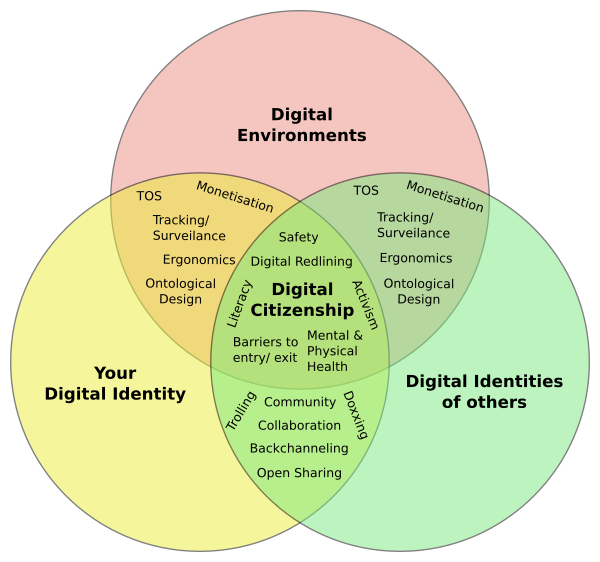
\includegraphics{assets/u5/Digital_citizenship_Venn.png}

\end{figure}%

\begin{tcolorbox}[enhanced jigsaw, toprule=.15mm, colback=white, colframe=quarto-callout-note-color-frame, arc=.35mm, opacityback=0, breakable, rightrule=.15mm, bottomrule=.15mm, leftrule=.75mm, left=2mm]

\emph{Note}: From ``Digital Citizenship,'' by A. Caines, 2016, August
25, \emph{Teaching in Higher Ed} {[}Podcast{]}
(https://teachinginhighered.com/podcast/digital-citizenship/)\{target=``\_blank''\}.
\href{https://creativecommons.org/licenses/by-nc-sa/4.0/}{CC BY-NC-SA
4.0}.

\end{tcolorbox}

\subsection{Activity: Refined Definition of Digital
Citizenship}\label{activity-refined-definition-of-digital-citizenship}

\begin{tcolorbox}[enhanced jigsaw, toprule=.15mm, colback=white, colframe=quarto-callout-note-color-frame, bottomtitle=1mm, leftrule=.75mm, coltitle=black, titlerule=0mm, rightrule=.15mm, colbacktitle=quarto-callout-note-color!10!white, left=2mm, title={Learning Activity}, opacitybacktitle=0.6, opacityback=0, breakable, toptitle=1mm, arc=.35mm, bottomrule=.15mm]

The purpose of this activity is to explore the elements of digital
citizenship with particular emphasis on those relevant to your academic
study.

Read through the following resources in order to refine your own
definition of what it means to be a digital citizen.

\begin{itemize}
\tightlist
\item
  \textbf{Online search:}

  \begin{itemize}
  \tightlist
  \item
    Read the introductory section of the Wikipedia article \emph{Digital
    Citizen} (2024).
  \item
    Conduct a general search for ``definition of digital citizen.''
    Choose the two best definitions and add these to the library of your
    citation management tool (Zotero or Obsidian),or keep a record for
    citation purposes.
  \item
    Locate one recent scholarly definition for ``digital citizen.''
    Record the reference for citation purposes. How recent is the
    reference?
  \end{itemize}
\item
  \textbf{Social media search:}

  \begin{itemize}
  \tightlist
  \item
    Explore recent tweets or posts (on X or whichever social media app
    you prefer) using the following hashtags: \#digitalcitizenship,
    \#digiciz, and \#digicit. Compile a list of elements relating to the
    concept of digital citizenship.
  \end{itemize}
\item
  \textbf{Read and identify:}

  \begin{itemize}
  \tightlist
  \item
    Read \emph{Nine Themes of Digital Citizenship} (2023), and search
    for other academic articles on digital citizenship using Google
    Scholar, LitMaps, or the TWU Library.
  \item
    Generate a table listing the nine elements of digital citizenship
    and identify a practical example of each element for your academic
    study. For example:
  \end{itemize}
\item
  \textbf{Define} digital citizenship

  \begin{itemize}
  \tightlist
  \item
    After completing the steps above, revise your personal description
    of digital citizenship. Does your new definition differ from your
    initial description?
  \end{itemize}
\item
  \textbf{Share} your insights. Share a reflection on this activity by
  posting either in your blog or on Discourse. For example:

  \begin{itemize}
  \tightlist
  \item
    I didn't realize the \ldots{} is part of digital citizenship because
    \ldots{}
  \item
    \ldots{} is not particularly relevant for university learners
    because \ldots{}
  \item
    \ldots{} is particularly relevant for university learners because
    \ldots{}
  \end{itemize}
\end{itemize}

\end{tcolorbox}

\subsubsection*{Rights and
Responsibilities}\label{rights-and-responsibilities}
\addcontentsline{toc}{subsubsection}{Rights and Responsibilities}

The concept of citizenship encompasses the rights and responsibilities
of individuals. We need to consider what rights and responsibilities
come with digital citizenship. In this mini challenge, we explore this
topic with particular emphasis on the rights and responsibilities
associated with learning in a digital age.

Following the hype of massive open online courses (MOOC) and the New
York Times declaring 2012 the
``\href{https://www.nytimes.com/2012/11/04/education/edlife/massive-open-online-courses-are-multiplying-at-a-rapid-pace.html}{year
of the MOOC},'' a small group of educators drafted \emph{A Bill of
Rights and Principles for Learning in a Digital Age} (Ng, 2013). This
document forms the basis for a course discussion on the rights and
responsibilities of digital citizens.

\subsection{Activity: Rights and Responsibilities of Digital
Citizens}\label{activity-rights-and-responsibilities-of-digital-citizens}

\begin{tcolorbox}[enhanced jigsaw, toprule=.15mm, colback=white, colframe=quarto-callout-note-color-frame, bottomtitle=1mm, leftrule=.75mm, coltitle=black, titlerule=0mm, rightrule=.15mm, colbacktitle=quarto-callout-note-color!10!white, left=2mm, title={Learning Activity}, opacitybacktitle=0.6, opacityback=0, breakable, toptitle=1mm, arc=.35mm, bottomrule=.15mm]

\begin{itemize}
\tightlist
\item
  \textbf{Search:} Conduct a general search for rights and
  responsibilities of digital citizenship to assist in refining your own
  list for university online study. Your search is likely to generate
  many results developed for the school sector, so you need to evaluate
  whether these rights and responsibilities are appropriate for you.
\item
  \textbf{Read}: Read the following and then conduct a search through
  the TWU library for digital rights and responsibilities.

  \begin{itemize}
  \tightlist
  \item
    \emph{A Bill of Rights and Principles for Learning in the Digital
    Age} (2013)
  \item
    \emph{`Bill of Rights' Seeks to Protect Students' Interests as
    Online Learning Rapidly Expands} (2013)
  \item
    \emph{Critique of 'Bill of Rights and Principles for Learning in the
    Digital Age} (2013)
  \end{itemize}
\item
  \textbf{Blog:} Prepare a table summarizing the primary rights and
  responsibilities for university learning in a digital age.
\item
  \textbf{Discuss:} Drawing on your knowledge and experience, join the
  discussion on Discourse regarding rights and responsibilities for
  learning in a digital age at TWU. You can discuss the topical issues
  listed below or add new ones to the forum. In each case, justify your
  position, taking opposing views into account.
\end{itemize}

\textbf{Topical Issues}

\begin{itemize}
\tightlist
\item
  Should higher education institutions have the right to determine what
  software applications learners should use for their studies?
\item
  Data generated by learners belongs to the learners, therefore should
  they have the right to access their data (for example forum discussion
  contributions) even after the course is completed?
\item
  Should higher education institutions reserve the right to ban
  disruptive learners from their learning platforms?
\item
  Where legally permissible, should learners have the right to access
  all course materials without the need to register a password?
\item
  Should higher education institutions have the right to limit the time
  required for completing a course?
\item
  Others?
\end{itemize}

We encourage you to reply and to ``like'' posts on Discourse. (Remember
to tag your posts using the course code: LDRS101).

\end{tcolorbox}

\subsubsection*{Personal and Professional
Identity}\label{personal-and-professional-identity}
\addcontentsline{toc}{subsubsection}{Personal and Professional Identity}

In short, digital citizenship is about being a person on the web. In the
previous unit on building your online presence we noted that individuals
portray different personas online; for example, personal, academic, and
professional.

On the one hand, we need to be careful about what we post online because
this can have a negative impact on future career prospects or current
employment. We must also be cognizant of the different limitations that
various careers place on what can be shared publicly and what needs to
stay private. On the other hand, building a strong learning or
professional network online is very powerful in staying up to date with
new trends and establishing connections with your peers.

In this section, we reflect on the balance between public and private in
a digital world, recognizing that this is going to be different for each
person depending on their own environments and professional
circumstances. We will also explore how like-minded professionals in
your field of interest network online.

\begin{quote}
The \ldots{} impact exercised by ICTs is due to at least four major
transformations: ``the blurring of the distinction between reality and
virtuality,'' `` the blurring of the distinction between human, machine
and nature,'' ``the reversal from information scarcity to information
abundance,'' and ``the shift from the primacy of stand-alone things,
properties, and binary relations, to the primacy of interactions,
processes and networks. (Floridi, 2015, p.~2)
\end{quote}

\subsection{Activity: Professional Online Identity and Digital
Citizenship}\label{activity-professional-online-identity-and-digital-citizenship}

\begin{tcolorbox}[enhanced jigsaw, toprule=.15mm, colback=white, colframe=quarto-callout-note-color-frame, bottomtitle=1mm, leftrule=.75mm, coltitle=black, titlerule=0mm, rightrule=.15mm, colbacktitle=quarto-callout-note-color!10!white, left=2mm, title={Learning Activity}, opacitybacktitle=0.6, opacityback=0, breakable, toptitle=1mm, arc=.35mm, bottomrule=.15mm]

In this activity we will explore professional online identity and
networking in the field of your choice.

\begin{itemize}
\tightlist
\item
  \textbf{Read}: First, scan the following resources:

  \begin{itemize}
  \tightlist
  \item
    \emph{High Court Rules Public Servants can be Sacked for Political
    Social Media Posts} (2019)
  \item
    \emph{'Think of Social Media as a Virtual Resumé, Expert Warns in
    Light of Health Board Resignation} (2017)
  \item
    You can also search online using the terms ``fired over tweet'' or
    ``social media firing cases.''
  \end{itemize}
\item
  \textbf{Watch}: Watch the short video
  \href{https://www.youtube.com/watch?v=EqSCR3HU4eg}{Watch: \emph{Using
  Twitter effectively in education - with Alec Couros}} Couros
  summarizes how educators are using Twitter (now X) to connect
  professionally.
\end{itemize}

\href{https://www.youtube.com/watch?v=EqSCR3HU4eg}{Watch: \emph{Using
Twitter effectively in education - with Alec Couros}}

\url{https://www.youtube-nocookie.com/embed/EqSCR3HU4eg}

\begin{itemize}
\tightlist
\item
  LinkedIN: Finally, visit the LinkedIn
  \href{https://www.linkedin.com/help/linkedin/answer/a544795}{help
  page} on finding and joining a LinkedIn group.\textbf{Questions to
  Consider}
\end{itemize}

After completing the activities above answer the following questions:

\begin{itemize}
\tightlist
\item
  How do like-minded professionals in your career or future career,
  field, or discipline network online (e.g., X, LinkedIn groups, other
  websites)?
\item
  What hashtags, if any, are being used for conversations in your chosen
  field?
\item
  What are the topical areas of discussion at the moment?
\item
  How could your field of interest improve professional networking
  online?
\item
  Do organizations in your field place restrictions on employees
  participating in social networks? (See for example \emph{Corporate
  Social Media Policies: The Good, the Mediocre, and the Ugly} (2010a),
  and \emph{More Social Media Policies: LA Times, Harvard Law,
  Microsoft, and Cisco} (2010b)\emph{.}
\end{itemize}

\end{tcolorbox}

\subsection{Activity: Blog: Professional Online Identity and Digital
Citizenship}\label{activity-blog-professional-online-identity-and-digital-citizenship}

\begin{tcolorbox}[enhanced jigsaw, toprule=.15mm, colback=white, colframe=quarto-callout-note-color-frame, bottomtitle=1mm, leftrule=.75mm, coltitle=black, titlerule=0mm, rightrule=.15mm, colbacktitle=quarto-callout-note-color!10!white, left=2mm, title={Learning Activity}, opacitybacktitle=0.6, opacityback=0, breakable, toptitle=1mm, arc=.35mm, bottomrule=.15mm]

Prepare a short blog post (about 300--400 words) summarizing your
findings on professional online networking in your field of interest.
Consider the following questions:

\begin{itemize}
\tightlist
\item
  How do like-minded professionals in your field network online and what
  do they talk about?
\item
  What does this mean for your online identity and being a digital
  citizen?
\end{itemize}

Remember to add a category or tag for your post using the course tag:
LDRS101.

\end{tcolorbox}

\subsection{Activity: Blog: My Online
Biography}\label{activity-blog-my-online-biography}

\begin{tcolorbox}[enhanced jigsaw, toprule=.15mm, colback=white, colframe=quarto-callout-note-color-frame, bottomtitle=1mm, leftrule=.75mm, coltitle=black, titlerule=0mm, rightrule=.15mm, colbacktitle=quarto-callout-note-color!10!white, left=2mm, title={Learning Activity}, opacitybacktitle=0.6, opacityback=0, breakable, toptitle=1mm, arc=.35mm, bottomrule=.15mm]

In this challenge you are asked to build or update your professional
online biography and the ``About'' page of your course blog.

\begin{itemize}
\tightlist
\item
  \textbf{Reflect} on the following online personas, target audiences,
  and how these will impact on the style and voice of the communication
  medium.
\end{itemize}

\begin{longtable}[]{@{}ll@{}}
\toprule\noalign{}
\textbf{Persona} & \textbf{Primary audience} \\
\midrule\noalign{}
\endhead
\bottomrule\noalign{}
\endlastfoot
Personal & Friends and family \\
Professional & (Future) Employers and professional network \\
Academic & Peer learning network \\
\end{longtable}

\begin{itemize}
\tightlist
\item
  \textbf{Choose} the most appropriate medium for each of your online
  personas, for example:
\end{itemize}

\begin{longtable}[]{@{}
  >{\raggedright\arraybackslash}p{(\columnwidth - 2\tabcolsep) * \real{0.2642}}
  >{\raggedright\arraybackslash}p{(\columnwidth - 2\tabcolsep) * \real{0.7358}}@{}}
\toprule\noalign{}
\begin{minipage}[b]{\linewidth}\raggedright
\textbf{Persona}
\end{minipage} & \begin{minipage}[b]{\linewidth}\raggedright
\textbf{Medium example}
\end{minipage} \\
\midrule\noalign{}
\endhead
\bottomrule\noalign{}
\endlastfoot
Personal & \href{https://www.facebook.com/}{Facebook} \\
Professional & \href{https://www.linkedin.com/}{Linkedin} \\
Academic & Learning blog or website \\
\end{longtable}

\begin{itemize}
\tightlist
\item
  \textbf{Identify} one or two professionals from your field of interest
  who maintain an active web presence and contribute regularly via
  social media. Explore their respective websites and professional
  listings as examples.

  \begin{itemize}
  \tightlist
  \item
    X (formerly Twitter) is a good place to search for individuals using
    popular hashtags from your field or area of study, for example,
    ``\#highereducation''
  \item
    Click through to their respective X user page. If they have a
    personal website listed on the user page visit the site and review
    their ``About'' page
  \item
    Visit their employer's page and try to locate their biography on the
    employer's website
  \item
    Search for the user on LinkedIn
  \item
    Compare the user information on these different sites. Observe how
    they link to social media account, and vary the style and content
    presented for the different personas
  \end{itemize}
\item
  \textbf{Create} or update your professional profile on LinkedIn.

  \begin{itemize}
  \tightlist
  \item
    Consult TWU's \emph{Student Resources} website (n.d.-b) which
    includes information about LinkedIn. TWU gives you access to
    LinkedIn Learning, which includes several great courses and videos,
    such as \emph{Rock Your LinkedIn Profile} (2024).
  \end{itemize}
\item
  \textbf{Create} or update your ``About'' page on your learning blog.
  You may prefer using a more informal style for this page aligned with
  your own personality and interests. Include links to your professional
  profile and respective links to social media that you use.
\item
  \textbf{Visit} the profile pages of your active social media accounts.
  Update if necessary, providing links back to your main page (for
  example, the ``About'' page on your website).
\item
  \textbf{Think carefully} about information you post publicly and keep
  a clear distinction between your personal online presence and your
  professional online persona. Review your privacy settings on your
  personal account(s).
\end{itemize}

\end{tcolorbox}

\section{Online Communities}\label{online-communities}

In this section we explore the topic of online communities and how we
can engage in social media to enhance our learning.

In the early years of the internet there was strong research interest in
studying the differences between virtual and real communities. However,
in more recent years we have observed a blurring of the boundaries
between online and real communities. In \emph{The Difference Between
Online \& Real Life Community?} Alison Michalk states:

\begin{quote}
Community boundaries are blurred to the extent that the Internet is
nothing more than a conduit for communication. The Internet is now just
another tool that we use to communicate within our various communities.
The same as we use mail, telephone and even a car to keep in touch with
our friends, family and colleagues. Our `real life communities' are not
mutually exclusive from our `online communities' given that it all comes
down to implied physical presence. (2013, para. 2)
\end{quote}

So how do we join and contribute constructively to these digital
communities? If you don't have much experience with online communities,
we encourage you to participate in the course forums and become an
active member of the TWU online learning community.

\subsubsection*{Research on Online
Communities}\label{research-on-online-communities}
\addcontentsline{toc}{subsubsection}{Research on Online Communities}

Research on the efficacy of online communities provides insights on
selecting productive communities and how to engage. Community
contributors can be classified into three types
\href{https://twu.idm.oclc.org/login?url=https://search.ebscohost.com/login.aspx?direct=true&db=edb&AN=100369742&site=eds-live&scope=site}{(Mocus
et al 2002)}):

\begin{enumerate}
\def\labelenumi{\arabic{enumi}.}
\tightlist
\item
  Core members are responsible for guiding the development of the
  community and have usually been involved with the community for a long
  time. These members have made significant contributions to the
  community's evolution and have earned leadership status. Frequently
  they also play an active role in moderation of the group.
\item
  Active members make regular contributions to the community.
\item
  Peripheral members occasionally contribute to the discussions and the
  periods of engagement are short and sporadic. ``Lurkers'', that is
  individuals seeking answers without making contributions, are normally
  associated with this group. The nature of engagement in a community is
  influenced by the community's life cycle stage
  \href{https://twu.idm.oclc.org/login?url=https://search.ebscohost.com/login.aspx?direct=true&db=edscma&AN=edscma.1459356&site=eds-live&scope=site}{A.
  Iriberri and G. Leroy 2009}:
\end{enumerate}

\begin{longtable}[]{@{}
  >{\raggedright\arraybackslash}p{(\columnwidth - 0\tabcolsep) * \real{0.9726}}@{}}
\toprule\noalign{}
\endhead
\bottomrule\noalign{}
\endlastfoot
\textbf{Life cycle }Characteristics** stage** ------------------
---------------------------------------------------- Inception stage
Focus is on determining the purpose, codes of conduct, funding and
sustainability \\
Creation stage User-centred design and evolution including issues of
privacy, anonymity, open versus closed communications \\
Growth stage Focus is on community building, for example, recruiting
members, growth management, integrating new members, trust building,
up-to-date content, interaction support, a few offline and online events
and meetings \\
Maturity stage By this stage a community culture will have emerged with
identifiable community leaders. Focus shifts to permeated management and
control, recognition of contributions, recognition of loyalty, member
satisfaction management and subgroup management. \\
\end{longtable}

Additional factors identified by the research to keep in mind include:

\begin{itemize}
\tightlist
\item
  \emph{Network cohesion}, that is the overall level of connections
  indicated by the network density has a positive impact on the core
  group as well as the success of the community (Toral et al
  2010).(Toral et al., 2009).
\item
  \emph{Network structure}. Successful communities need a critical mass
  of contributors, however there is no fixed number that determines
  success. Most communities can expect between 45--90 \% of nonactive
  members, but communities with a strong and experienced core group will
  have a positive impact on success (Nonnecke \& Preece, 2000, as cited
  in Toral et al., 2009). Moreover, the positive effects of network
  structure on participation persist irrespective of the life cycle
  stage of the community, and activity participation influences network
  structure (Igl 2014).(Igl, 2014).
\item
  \emph{Centralization}. Communities with a high degree of
  centralization and control exert a negative impact on all
  participation variables (Igl, 2014).
\end{itemize}

\subsubsection*{Practical Implications}\label{practical-implications}
\addcontentsline{toc}{subsubsection}{Practical Implications}

There are many online communities, and it will be worth your effort in
doing a little online research to determine the network cohesion and
network structure of the community. You will be able to determine this
by reviewing the archive history. Avoid communities with overly
centralized control; in the long run, they are not likely to be
productive.

When joining an online community try to identify its life cycle stage by
scanning the archive of posts. Young communities are likely to be more
tolerant of newbie questions, as responses to these questions will
provide support resources for new members in the future. It's a good
idea to search the forum for your answer before posting a question.
Don't be surprised if newbie questions go unanswered in mature
communities; they may can even attract curt rebuttals. If you're a
longstanding member of the community, post a tactful reply, for example,
``Your question has already been answered'' and post a link to the
appropriate reply.

The best advice when joining a new community is to lurk for a while
before introducing yourself so that you can become familiar with the
culture and practices of the community. Fill out your profile page on
the forum site, rather than posting a biography in the main discussion
threads. Of course, if the community is in the creation phase, you may
want to play a more active role in building the community and becoming
part of the core contributors.

\subsubsection*{Communities of Practice}\label{communities-of-practice}
\addcontentsline{toc}{subsubsection}{Communities of Practice}

As you continue to reflect on your social network and consider other
learning networks to join for personal or professional growth, we want
to present another framing of an online community called a
\emph{community of practice}.

\begin{quote}
A community of practice is a group of people who \emph{``share a concern
or a passion for something they do and learn how to do it better as they
interact regularly.''} (Wenger-Trayner, 2022)
\end{quote}

Cognitive anthropologists Jean Lave and Etienne Wenger coined the term
community of practice when studying apprenticeships as a learning
model---the term referred to the community that acts as a living
curriculum. Once the concept was articulated the researchers started to
see communities everywhere, even when no formal apprenticeship system
existed.

The basic premise behind communities of practice is simple: we all learn
in everyday life from the communities in which we find ourselves.
Communities of practice are everywhere. Nearly everyone belongs to some
community of practice, whether it is through our working colleagues or
associates, our profession or trade, or our leisure interests, such as a
book club. Wenger-Trayner (2022) argues that a community of practice is
different from a community of interest or a geographical community in
that it involves a shared practice: ways of doing things that are shared
to some significant extent among members.

\subsubsection*{Characteristics of a Community of
Practice}\label{characteristics-of-a-community-of-practice}
\addcontentsline{toc}{subsubsection}{Characteristics of a Community of
Practice}

According to Wenger-Treyner (2022) there are three crucial
characteristics of a community of practice:

\begin{enumerate}
\def\labelenumi{\arabic{enumi}.}
\tightlist
\item
  \textbf{Domain:} A common interest that connects and holds together
  the community;
\item
  \textbf{Community:} A community is bound by the shared activities they
  pursue (for example, meetings, discussions) around their common
  domain;
\item
  \textbf{Practice:} Members of a community of practice are
  practitioners; what they do informs their participation in the
  community; and what they learn from the community affects what they
  do.Wenger- Treyner has argued that although individuals learn through
  participation in a community of practice, more important is the
  generation of newer or deeper levels of knowledge through the sum of
  the group activity. If the community of practice is centered around
  business processes, for instance, this can be of considerable benefit
  to an organization.
\end{enumerate}

\subsubsection*{Types of Communities of
Practice}\label{types-of-communities-of-practice}
\addcontentsline{toc}{subsubsection}{Types of Communities of Practice}

Today, communities of practices are increasingly being used to improve
knowledge management and connect people within business, government,
education, and other organizations.

The design of the community will look different depending on the purpose
and needs of the participants. There are four basic types of
communities:

\begin{itemize}
\tightlist
\item
  \textbf{Helping communities} provide a forum for community members to
  help each other with everyday work needs
\item
  \textbf{Best practice communities} develop and disseminate best
  practices, guidelines, and strategies for their members' use
\item
  \textbf{Knowledge stewarding communities} organize, manage, and
  steward a body of knowledge from which community members can draw
\item
  \textbf{Innovation communities} create breakthrough ideas, new
  knowledge, and new practices
\end{itemize}

As you reflect on digital practices in university and the workplace,
consider how engaging in a community of practice could benefit you as a
learner and in your future career.

\subsection{Activity: What Is a Community of
Practice?}\label{activity-what-is-a-community-of-practice}

\begin{tcolorbox}[enhanced jigsaw, toprule=.15mm, colback=white, colframe=quarto-callout-note-color-frame, bottomtitle=1mm, leftrule=.75mm, coltitle=black, titlerule=0mm, rightrule=.15mm, colbacktitle=quarto-callout-note-color!10!white, left=2mm, title={Learning Activity}, opacitybacktitle=0.6, opacityback=0, breakable, toptitle=1mm, arc=.35mm, bottomrule=.15mm]

\begin{itemize}
\tightlist
\item
  \textbf{Watch}: \emph{Communities of Practice (Etienne and Beverly
  Wenger-Trayner)} (2022)
\end{itemize}

\href{https://www.youtube.com/watch?v=SmqLyOLIjos}{Watch:
\emph{Communities of Practice (Etienne and Beverly Wenger-Trayner)}}

\url{https://www.youtube-nocookie.com/embed/SmqLyOLIjos}

\begin{itemize}
\tightlist
\item
  \textbf{Read}: To learn more about the origins and theory of
  communities of practice, see \emph{Introduction to Communities of
  Practice} (2015)
\end{itemize}

Feel free to discuss your topics of interest in Discourse, or search
online for communities of practice that interest you.

\end{tcolorbox}

\section{Connecting and Learning Through Social
Media}\label{connecting-and-learning-through-social-media}

\subsection{Activity: Mapping My Social
Network}\label{activity-mapping-my-social-network}

\begin{tcolorbox}[enhanced jigsaw, toprule=.15mm, colback=white, colframe=quarto-callout-note-color-frame, bottomtitle=1mm, leftrule=.75mm, coltitle=black, titlerule=0mm, rightrule=.15mm, colbacktitle=quarto-callout-note-color!10!white, left=2mm, title={Learning Activity}, opacitybacktitle=0.6, opacityback=0, breakable, toptitle=1mm, arc=.35mm, bottomrule=.15mm]

Online communities are varied and can be categorized by their purpose:
social, academic, professional, and so on. For this activity, we
encourage you to consider your purpose in building an online community.

What are your goals?

\begin{itemize}
\tightlist
\item
  Do you want to connect with TWU peers internationally and in Canada?
  Is your focus on academic support or building personal relationships?
\item
  Are you interested in the communities that relate to your chosen
  profession? If so, do a quick search for online communities for a
  career that interests you (e.g., for businesses: 15 Best Online
  Community Platforms of 2023 (Ranked)).
\item
  Do you want to engage with online communities that align with your
  personal interests? (e.g., sports, arts, politics, gardening, coding)
\item
  \textbf{Write:} Write down your goals for joining an online community.
  Next, consider the networks you are currently a part of. You may want
  to refer back to Unit 1 in which you created a Personal Learning
  Network map.
\item
  \textbf{Map}: Now, with a focus on networking create your own Social
  Map. See the following example from Brian Solis, a digital analyst,
  anthropologist and author.
\end{itemize}

\begin{figure}[H]

\caption{\label{fig-2374839848x2769ef5f1a}Brian Solis Online: Social Map
}

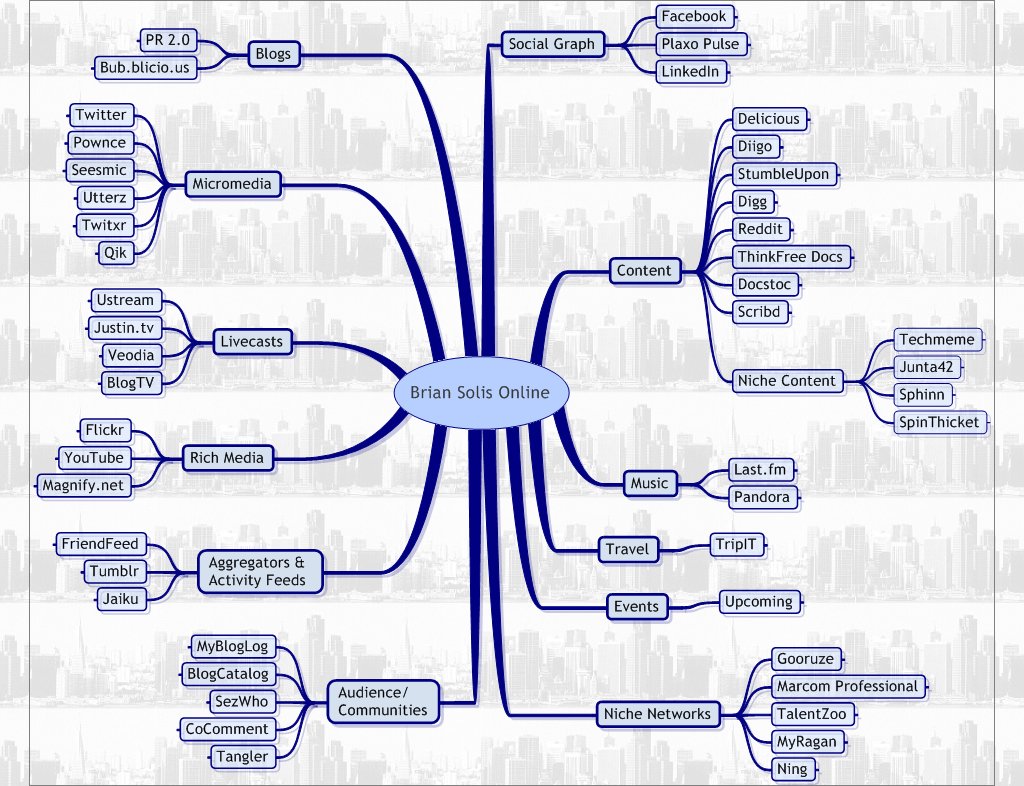
\includegraphics{assets/u5/social_map.png}

\end{figure}%

\emph{Note}: From ``Brian Solis Online,'' by B. Solis, March 30, 2008,
\emph{@BRIANSOLIS} (\href{https://briansolis.com/}{Homepage - Brian
Solis}). \href{https://creativecommons.org/licenses/by/2.0/}{CC BY 2.0.}
- Finally, \textbf{reflect} on the social media technologies you use for
learning and how these impact your digital footprint and online
identity.

\end{tcolorbox}

\subsubsection{Collaboration and Annotation
Tools}\label{collaboration-and-annotation-tools}

Another way to join an online community or discussion forum is to
annotate the web. Hypothes.is is one tool used at TWU for students to
collaborate and discuss online resources.

Hypothes.is an open source platform that allows users to annotate any
website, communicate with others, and collaborate with peers.

\subsection{Activity: Introduction To
Hypothes.is}\label{activity-introduction-to-hypothes.is}

\begin{tcolorbox}[enhanced jigsaw, toprule=.15mm, colback=white, colframe=quarto-callout-note-color-frame, bottomtitle=1mm, leftrule=.75mm, coltitle=black, titlerule=0mm, rightrule=.15mm, colbacktitle=quarto-callout-note-color!10!white, left=2mm, title={Learning Activity}, opacitybacktitle=0.6, opacityback=0, breakable, toptitle=1mm, arc=.35mm, bottomrule=.15mm]

\begin{itemize}
\tightlist
\item
  \textbf{Read}: Go to the Hypothes.is website and have a quick read to
  see what the tool is and how it works.
\item
  \textbf{Watch}: \emph{How to Annotate the Web with Hypothes.is} (2017)
\end{itemize}

\href{https://www.youtube.com/watch?v=e235JwmmEcQ}{Watch: \emph{How to
Annotate the Web with hypothes.is}}

\url{https://www.youtube-nocookie.com/embed/e235JwmmEcQ}

Finally, skim these articles highlighting the benefits of using
annotative tools such as Hypothes.is:

\begin{itemize}
\tightlist
\item
  \href{https://twu.idm.oclc.org/login?url=https://search.ebscohost.com/login.aspx?direct=true&db=edsdoj&AN=edsdoj.12d6cddd34714c51bc1f6f8d6d9dea39&site=eds-live&scope=site}{\emph{Sharing
  Notes Is Encouraged: Annotating and Cocreating with Hypothes.is and
  Google Docs}} (2021)
\item
  {[}\emph{Jottings in the Margins - Using Digital Annotation to Support
  21st Century Learning}{]}
  (https://www.thescopes.org/assets/scopes/SCOPE\_104-Wood\_LT9.pdf)\{target=``\_blank''\}(2020)
\end{itemize}

\end{tcolorbox}

\subsection{Activity: Annotating and Collaborating in
Hypothes.is}\label{activity-annotating-and-collaborating-in-hypothes.is}

\begin{tcolorbox}[enhanced jigsaw, toprule=.15mm, colback=white, colframe=quarto-callout-note-color-frame, bottomtitle=1mm, leftrule=.75mm, coltitle=black, titlerule=0mm, rightrule=.15mm, colbacktitle=quarto-callout-note-color!10!white, left=2mm, title={Learning Activity}, opacitybacktitle=0.6, opacityback=0, breakable, toptitle=1mm, arc=.35mm, bottomrule=.15mm]

In this activity, we will practice using Hypothes.is by annotating an
article on the difference between digital skills and digital literacies.

\begin{itemize}
\item
  \emph{Quick-Start Guide for Students} \textbf{Open account}: Read the
  Hypothes.is (2023b) \emph{How to use Hypothes.is on Mobile Devices}
  and create an account on Hypothes.is. We recommend that you use the
  Chrome browser and install the Hypothes.is extension. Alternatively,
  you can annotate web pages directly from the Hypothes.is website by
  pasting the link into the text area after you have logged into the
  site. If you are working on a mobile device, please follow these
  instructions: (2023a).
\item
  \textbf{Read}: \emph{Knowing the Difference Between Digital Skills and
  Digital Literacies, and Teaching Both} (2016)
\item
  \textbf{Annotate}: Activate annotations after logging in to
  Hypothes.is---click the search icon () and enter the course code
  (LDRS101) to filter posts for this course from the public feed.
  Annotate or reply to posts by visiting the annotation page (you will
  need to be logged into the Hypothes.is site to post).
\end{itemize}

Remember to tag your posts using the course code: LDRS101 (the course
tag is required to harvest posts for the course feed).

\end{tcolorbox}

\subsection{Activity: Hypothes.is
Challenge!}\label{activity-hypothes.is-challenge}

\begin{tcolorbox}[enhanced jigsaw, toprule=.15mm, colback=white, colframe=quarto-callout-note-color-frame, bottomtitle=1mm, leftrule=.75mm, coltitle=black, titlerule=0mm, rightrule=.15mm, colbacktitle=quarto-callout-note-color!10!white, left=2mm, title={Learning Activity}, opacitybacktitle=0.6, opacityback=0, breakable, toptitle=1mm, arc=.35mm, bottomrule=.15mm]

In this course we have provided numerous articles, websites, videos, and
other resources to support your learning. Perhaps you have added these
resource links to Obsidian or Zotero for future reference (e.g.,
preparing for citations needed for course assignments).

Here is one more step we encourage you to take advantage of:

\begin{itemize}
\tightlist
\item
  Review the course learning outcomes.
\item
  Refer to the Course Book table of contents and look at the Unit
  topics, subtopics, and activities listed.
\item
  Recall any resources that stood out to you. What article, video, or
  website do you want to engage with further? What key points would you
  like to discuss with your peers?
\item
  Select three or more resources to reread and annotate using
  Hypothes.is.
\item
  Reply to posts by visiting the annotation page (you will need to be
  logged into the Hypothes.is site to post).
\end{itemize}

Remember to tag your posts using the course code: LDRS101.

\end{tcolorbox}

\subsection{Activity: Social Media for Connecting and
Learning}\label{activity-social-media-for-connecting-and-learning}

\begin{tcolorbox}[enhanced jigsaw, toprule=.15mm, colback=white, colframe=quarto-callout-note-color-frame, bottomtitle=1mm, leftrule=.75mm, coltitle=black, titlerule=0mm, rightrule=.15mm, colbacktitle=quarto-callout-note-color!10!white, left=2mm, title={Learning Activity}, opacitybacktitle=0.6, opacityback=0, breakable, toptitle=1mm, arc=.35mm, bottomrule=.15mm]

In this activity we will explore how social media can support online
learning and engagement.

\begin{itemize}
\tightlist
\item
  \emph{Social Media for Learning} \textbf{Read}: (n.d.)
\item
  \textbf{Watch:} \emph{Building More Creative Social Networks} (2020)
\end{itemize}

\href{https://www.youtube.com/watch?v=Acc4zY1sQ0o}{Watch: \emph{Building
More Creative Social Networks}}

\url{https://www.youtube-nocookie.com/embed/Acc4zY1sQ0o}

\begin{itemize}
\tightlist
\item
  \emph{The Conversation Prism} \textbf{Explore}: Check out (2008) and
  also refer to the graphic below listing numerous apps for listening,
  learning, and adapting (click the graphic to enlarge).
\end{itemize}

Feel free to annotate the articles you read or reply to annotations
using Hypothes.is. Remember to tag your posts using the course code:
LDRS101.

\emph{The Conversation Prism}

{[}Alt text: colourful segmented circle containing many media apps{]}

\begin{figure}[H]

\caption{\label{fig-11327713066xc661527cef}A colorful circular chart
with many different colored icons Description automatically generated
with medium confidence}

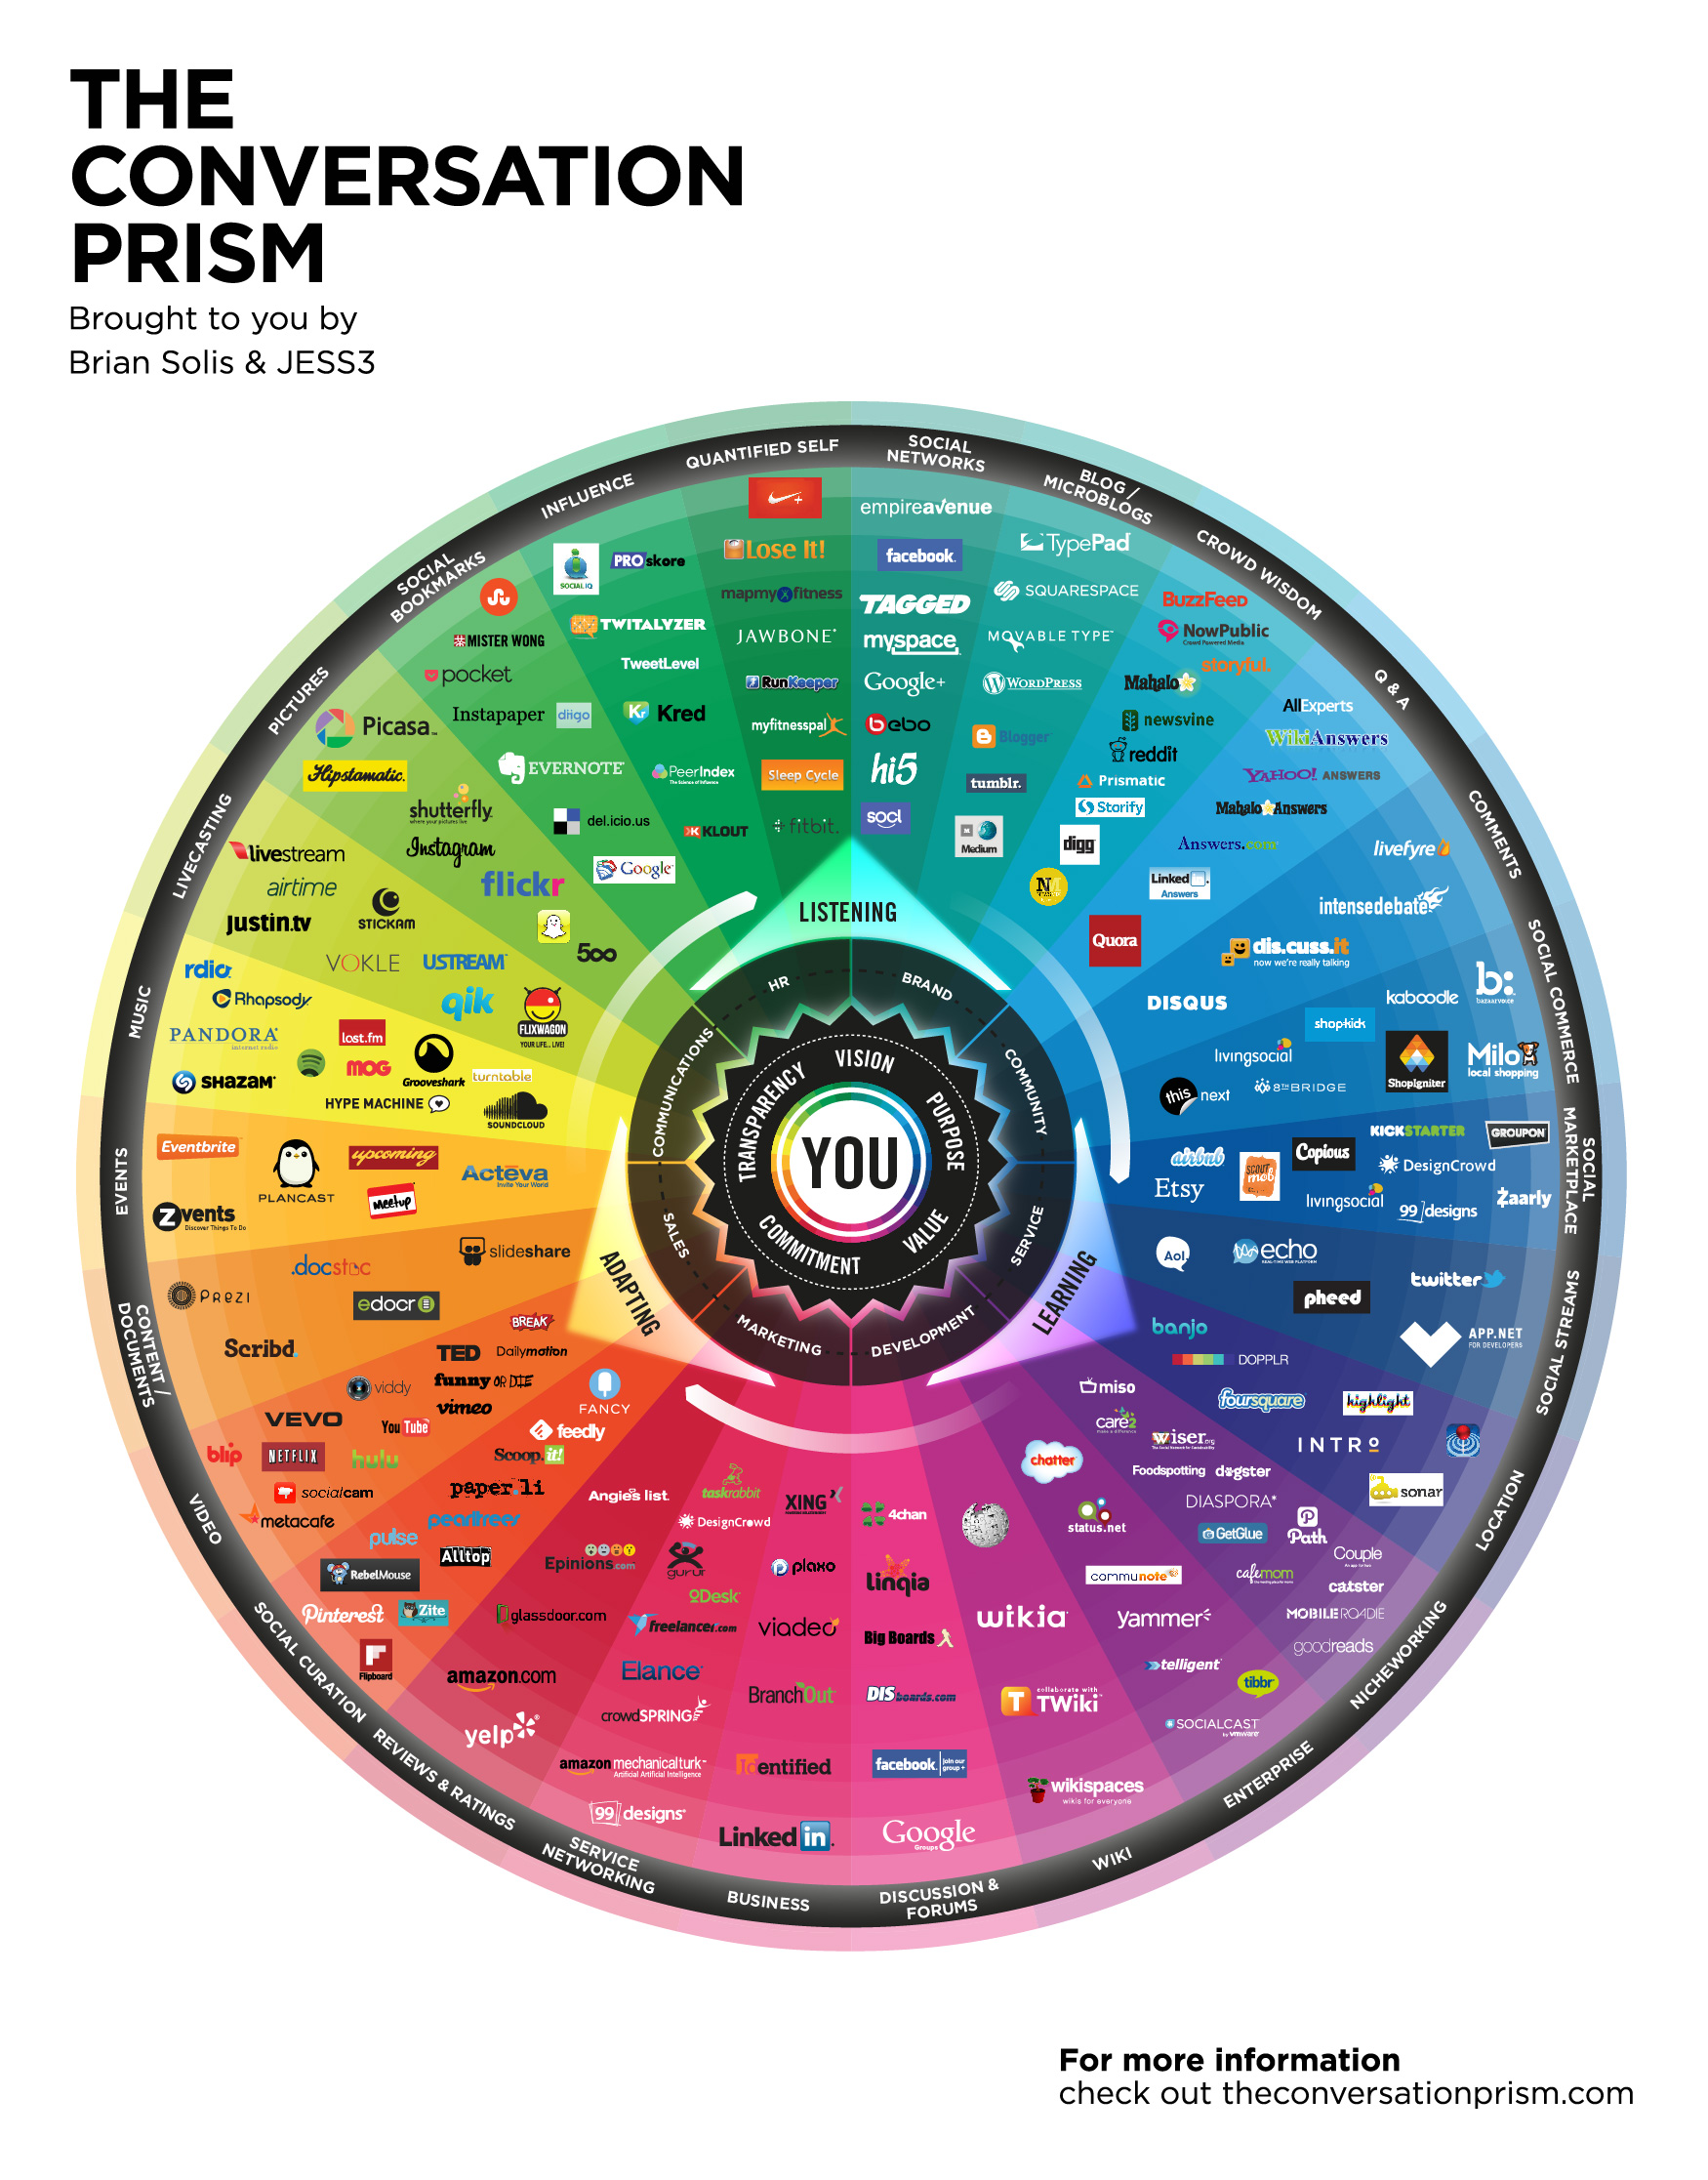
\includegraphics{assets/u5/conversation_prism.jpg}

\end{figure}%

\begin{quote}
\emph{Note:} From ``Conversations Prism 4'' by SolucionaFacil.es,
December 12, 2013, Flickr
(https://flickr.com/photos/solucionafacil/11327713066/). CC BY-ND 2.0.
\end{quote}

\end{tcolorbox}

\subsection{Activity: Social Media, Online Identity, and
Learning}\label{activity-social-media-online-identity-and-learning}

\begin{tcolorbox}[enhanced jigsaw, toprule=.15mm, colback=white, colframe=quarto-callout-note-color-frame, bottomtitle=1mm, leftrule=.75mm, coltitle=black, titlerule=0mm, rightrule=.15mm, colbacktitle=quarto-callout-note-color!10!white, left=2mm, title={Learning Activity}, opacitybacktitle=0.6, opacityback=0, breakable, toptitle=1mm, arc=.35mm, bottomrule=.15mm]

\begin{itemize}
\tightlist
\item
  \textbf{Write}: Join the Discourse forum on social media, online
  identity, and learning by sharing your personal views and thoughts.
  Choose one or more of the following questions as a catalyst for your
  contributions to the forum:

  \begin{itemize}
  \tightlist
  \item
    How much of what you learn should be open and transparent (i.e.,
    public) and how much should be kept private? Why?
  \item
    In a digital age, how important is it for you to build a digital
    footprint of your learning?
  \item
    What are the challenges and opportunities for building your online
    identity?
  \item
    What levels of online engagement do you feel are appropriate for
    your own learning on this course? Does this differ from your
    engagement in other online communities?
  \item
    Other?
  \end{itemize}
\end{itemize}

\begin{quote}
Like, share and reply to posts. These are forms of engagement and a
contribution to your online learning identity. Remember to tag your
posts using the course code: LDRS101.
\end{quote}

\end{tcolorbox}

\section{Connecting to the TWU
Community}\label{connecting-to-the-twu-community}

Our final topic focuses on the TWU community and how you can participate
both online and on campus. As a TWU student you have the opportunity to
connect with a diverse student body, faculty, and staff. What role does
technology play in how you communicate with your peers, collaborate on
projects, and build relationships?

In this unit we have discussed what it means to be a digital citizen and
how we can engage with online communities. How does this apply to you as
a TWU student? As we wrap up this unit, we encourage you to reflect on
your personal and academic goals and how you can engage with the TWU
community.

5.4.1 Activity: TWU's Learning Community

\begin{tcolorbox}[enhanced jigsaw, toprule=.15mm, colback=white, colframe=quarto-callout-note-color-frame, bottomtitle=1mm, leftrule=.75mm, coltitle=black, titlerule=0mm, rightrule=.15mm, colbacktitle=quarto-callout-note-color!10!white, left=2mm, title={Learning Activity}, opacitybacktitle=0.6, opacityback=0, breakable, toptitle=1mm, arc=.35mm, bottomrule=.15mm]

\begin{itemize}
\tightlist
\item
  \textbf{Read}: Take a moment to reread the course description for this
  course:
\end{itemize}

\begin{quote}
Introduces theories and competencies related to learning and thriving in
a digital world. Explores how learners are situated in ``the digital''
throughout their lives and how they can use digital technologies to
enhance and enrich their experience of learning, working, and playing.
Learners will begin to build a curated digital footprint, initiate and
develop personal and professional learning networks; develop
competencies to allow them to evaluate and choose digital platforms and
tools that are safe and ethical; and explore how to use digital
technologies to discover, curate, connect, and share knowledge with
their communities.
\end{quote}

Next, focus on two key course learning outcomes:

\begin{itemize}
\tightlist
\item
  Develop personal and professional learning networks to discover and
  share knowledge, collaborate with others, and become engaged digital
  global citizens.
\item
  Create inclusive digital communities which embody a sense of
  belonging, connection, and Christian hospitality.
\end{itemize}

Finally, take a look at Trinity's \emph{Life at TWU} (n.d.-a) website.

\begin{quote}
We invite all TWU students to connect, thrive, and serve in a dynamic,
Christ-centred learning community where they can develop as maturing
disciples, thoughtful global citizens, and compassionate servant
leaders. \emph{Experience life and learning here.}
\end{quote}

\begin{itemize}
\tightlist
\item
  \textbf{Reflect}: How might you connect, thrive, and serve through
  your connections and contributions online, and if applicable, on
  campus?
\end{itemize}

What experiences have you had so far in connecting with your peers and
getting to know the TWU community? If you have not participated in the
engagement opportunities presented in this course (Discourse, WordPress
blog), take the time now to connect!

\textbf{TWU on Social Media}

Here are some other websites you might want to check out for more about
the TWU community:

\begin{itemize}
\tightlist
\item
  TWU Facebook
\item
  X (Twitter)
\item
  Instagram
\item
  \textbf{Write}: Jot down your responses to the following questions in
  your reflective journal (Obsidian):
\item
  What are your personal and academic goals for making connections at
  TWU?
\item
  What steps will you take to make those connections?
\item
  What technology or digital skills will you need to fully engage?
\item
  How can connecting to the TWU community enhance your understanding of
  digital citizenship and online networking?
\end{itemize}

\end{tcolorbox}

\section{Summary}\label{summary-4}

In this unit you have had the opportunity to learn what it means to be a
digital citizen, including the rights and responsibilities we should
abide by. You have had the opportunity to explore and connect with an
online community and have reflected on your personal and academic goals
for networking. Finally, you have considered your role as a TWU student
and how you might build connections with peers, faculty, and staff. As
we move on to our final unit, consider how you might share your
knowledge online and create an inclusive digital community.

\begin{tcolorbox}[enhanced jigsaw, toprule=.15mm, colback=white, colframe=quarto-callout-note-color-frame, bottomtitle=1mm, leftrule=.75mm, coltitle=black, titlerule=0mm, rightrule=.15mm, colbacktitle=quarto-callout-note-color!10!white, left=2mm, title={Checking Your Learning}, opacitybacktitle=0.6, opacityback=0, breakable, toptitle=1mm, arc=.35mm, bottomrule=.15mm]

Before you move on to the next unit check that you are able to:

Discuss the dimensions of digital citizenship for work and learning in
the 21st century and how these differ from the offline
environmentOutline the rights and responsibilities of a digital
citizenExplore professional online identity and networking in the field
of your choiceReflect on the balance between public and private in a
digital worldEvaluate a range of social media, technologies, and
communities appropriate for supporting learningDevelop online learning
networks to discover and share knowledge, collaborate with others, and
become engaged digital global citizensConsider how you might connect,
thrive, and serve in the TWU learning community :::

\end{tcolorbox}

\bookmarksetup{startatroot}

\chapter{Sharing Your Knowledge}\label{sharing-your-knowledge}

\section*{Overview}\label{overview-5}
\addcontentsline{toc}{section}{Overview}

\markright{Overview}

Congratulations! You've made it to the final unit in our course,
\emph{Learning with Technology}. In this last unit we will have a chance
to explore some digital tools that you may encounter in your academic
studies at TWU. We'll look at how these skills translate to preparing
you for the workplace and will examine the role technology plays in your
chosen field of study. You'll also have the opportunity to research some
current events related to societal issues and the internet and will
discuss how to address these challenges. Finally, we'll conclude our
course with a discussion on digital wisdom. As you begin this unit, here
are some guiding questions to consider:

\begin{itemize}
\tightlist
\item
  How will my use of technology support my social, academic, and
  spiritual goals?
\item
  How will I share my knowledge and skills to engage as a digital global
  citizen?
\item
  How will I connect and collaborate with others as part of an inclusive
  digital community?
\end{itemize}

\subsection*{Topics}\label{topics-5}
\addcontentsline{toc}{subsection}{Topics}

This unit is divided into the following topics:

\begin{enumerate}
\def\labelenumi{\arabic{enumi}.}
\tightlist
\item
  Sharing your learning at TWU
\item
  Digital practices in the workplace
\item
  Societal issues and the internet
\item
  Digital wisdom
\end{enumerate}

\subsection*{Learning Outcomes}\label{learning-outcomes-4}
\addcontentsline{toc}{subsection}{Learning Outcomes}

When you have completed this unit you will be able to:

\begin{itemize}
\tightlist
\item
  Discuss how technology has changed business practices in your field of
  interest or career
\item
  Utilize technology to discover and share knowledge, collaborate with
  others, and become engaged digital global citizens
\item
  Describe societal issues and problematic online behaviours which have
  emerged in the digital world, and how to deal with these challenges in
  an ethical manner
\item
  Create inclusive digital communities which embody a sense of
  belonging, connection, and Christian hospitality
\item
  Create a personalized narrative to document and express your learning
  process
\item
  Practice evaluative judgment to document your process of learning in
  complex domains of knowledge
\end{itemize}

\subsection*{Activity Checklist}\label{activity-checklist-5}
\addcontentsline{toc}{subsection}{Activity Checklist}

Here is a checklist of learning activities you will benefit from in
completing this unit. You may find it useful for planning your work.

\begin{tcolorbox}[enhanced jigsaw, toprule=.15mm, colback=white, colframe=quarto-callout-note-color-frame, bottomtitle=1mm, leftrule=.75mm, coltitle=black, titlerule=0mm, rightrule=.15mm, colbacktitle=quarto-callout-note-color!10!white, left=2mm, title={Learning Activity}, opacitybacktitle=0.6, opacityback=0, breakable, toptitle=1mm, arc=.35mm, bottomrule=.15mm]

\textbf{Learning Activities}

\begin{itemize}
\tightlist
\item
  Watch the video
  \href{https://www.youtube.com/watch?v=iY4UhfQefdU}{Higher Ed Trends:
  Student Career Anxiety and the Future of Work} (2015)
\item
  Read the articles on how the internet impacted the newspaper and music
  industries.
\item
  Discuss the impact of digital technology on business.
\item
  Explore AI tools for university students and view the resources
  provided.
\item
  View the resources on AI and plagiarism.
\item
  Discuss the impact of automation and AI in the workplace.
\item
  View the resources on the price of AI and discuss the ethical
  implications.
\item
  Explore the topics focusing on societal issues on the internet,
  including website tracking, trolling, net neutrality, and equity.
\item
  Publish an editorial on your blog about an issue that interests you.
\item
  Read the article on digital wisdom and reflect on how technology
  serves both personal and communal benefits.
\end{itemize}

\begin{tcolorbox}[enhanced jigsaw, toprule=.15mm, colback=white, colframe=quarto-callout-note-color-frame, arc=.35mm, opacityback=0, breakable, rightrule=.15mm, bottomrule=.15mm, leftrule=.75mm, left=2mm]

\emph{\textbf{Notes}:}

\begin{itemize}
\tightlist
\item
  \emph{You will be directed to complete these activities as they come
  up in the unit.}
\item
  \emph{The learning activities in this course are designed to prepare
  you for the graded assignments in this course. You are strongly
  encouraged to complete them.}
\end{itemize}

\end{tcolorbox}

\end{tcolorbox}

\begin{tcolorbox}[enhanced jigsaw, toprule=.15mm, colback=white, colframe=quarto-callout-note-color-frame, arc=.35mm, opacityback=0, breakable, rightrule=.15mm, bottomrule=.15mm, leftrule=.75mm, left=2mm]

\textbf{Assessment}

\begin{itemize}
\tightlist
\item
  \emph{See the Assessment section in Moodle for assignment details.}
\end{itemize}

\end{tcolorbox}

\subsection*{Resources}\label{resources-5}
\addcontentsline{toc}{subsection}{Resources}

\begin{itemize}
\tightlist
\item
  All resources will be provided online in the unit.
\end{itemize}

\begin{tcolorbox}[enhanced jigsaw, toprule=.15mm, colback=white, colframe=quarto-callout-note-color-frame, arc=.35mm, opacityback=0, breakable, rightrule=.15mm, bottomrule=.15mm, leftrule=.75mm, left=2mm]
\begin{minipage}[t]{5.5mm}
\textcolor{quarto-callout-note-color}{\faInfo}
\end{minipage}%
\begin{minipage}[t]{\textwidth - 5.5mm}

\textbf{\emph{Resource Reminders}}

\begin{itemize}
\tightlist
\item
  Remember to continuously add resources that align with your learning
  goals to your Zotero library.
\item
  Utilize your community---peers, coworkers, and online communities---as
  valuable resources! Stay engaged to seek assistance and exchange
  helpful resources and insights.
\end{itemize}

\end{minipage}%
\end{tcolorbox}

\section{Sharing Your Learning at
TWU}\label{sharing-your-learning-at-twu}

Community is an essential component of Trinity Western University. Just
have a look at the \href{https://www.twu.ca/}{TWU website} and you will
find several references to learning within a community. For example:

\begin{quote}
At Trinity Western University, you'll experience an authentic and
engaging community as you enrich your understanding of the
world---preparing for a life of faithful engagement in your community
and profession. We are deeply committed to providing a transformational
education, where you will develop practical professional skills while
exploring bigger ideas about who you are, what you believe, and what
you're called to do in the world. (Trinity Western University, n.d.-c)
\end{quote}

Why is community so important to TWU, and how does it help us learn?
Have a quick read about TWU's
\href{https://www.twu.ca/about-us/commitments/core-values}{Core Values}
(n.d.-b). At this point in the course, we hope you have taken full
advantage of the online community and have personal examples of how
these interactions have impacted you.

As for learning \ldots{} how does sharing our learning within a
community help us achieve our personal and professional goals?

There are several social learning theories and practices that explain
how social interactions impact our learning (e.g., situated learning,
social constructivism, connectivism, cooperative and collaborative
learning, communities of inquiry, and so on). If you're interested, feel
free to look these up online or use tools such as LitMaps.

In this course we have promoted the use of tools that allow you to share
your learning online: Discourse, Hypothes.is, and WordPress. Our goal is
to help you utilize technology to discover and share knowledge,
collaborate with others, and become engaged digital global citizens. In
the next activity, we ask you to reflect on your learning experiences
and your goals.

\subsection{Activity: Learning in
Community}\label{activity-learning-in-community}

\begin{tcolorbox}[enhanced jigsaw, toprule=.15mm, colback=white, colframe=quarto-callout-note-color-frame, bottomtitle=1mm, leftrule=.75mm, coltitle=black, titlerule=0mm, rightrule=.15mm, colbacktitle=quarto-callout-note-color!10!white, left=2mm, title={Learning Activity}, opacitybacktitle=0.6, opacityback=0, breakable, toptitle=1mm, arc=.35mm, bottomrule=.15mm]

\begin{itemize}
\tightlist
\item
  \textbf{Read}: Here are several resources that explain how we learn in
  community.

  \begin{itemize}
  \tightlist
  \item
    \href{https://openpress.usask.ca/humanmooc/chapter/social-learning-in-online-environments/}{Social
    Learning in Online Environments} (n.d.)
  \item
    \href{https://socialsci.libretexts.org/Bookshelves/Education_and_Professional_Development/Teaching_Crowds_-_Learning_and_Social_Media_(Dron_and_Anderson)\%7Btarget=\%22_blank\%22\%7D/02\%3A_Social_Learning_Theories}{Social
    Learning Theories} (2021)
  \item
    \href{https://www.sciencedirect.com/science/article/abs/pii/S0360131516300872}{Social
    Networking, Knowledge Sharing, and Student Learning: The Case of
    University Students} (2016)
  \item
    \href{https://www.ncbi.nlm.nih.gov/pmc/articles/PMC5132366/}{Collaborative
    Learning in Higher Education: Evoking Positive Interdependence}
    (2016)
  \end{itemize}
\item
  \textbf{Watch}:
  \href{https://www.youtube.com/watch?v=AB-_822TRms}{What is Social
  Learning?} (2017)
\end{itemize}

\url{https://www.youtube-nocookie.com/embed/AB-_822TRms}

\begin{itemize}
\tightlist
\item
  At TWU you may be asked to participate in various group activities,
  such as group work, partner projects, team presentations, and so on.
  Have a look at this resource that explains examples and reasons for
  these activities:
\item
  \href{https://cft.vanderbilt.edu/guides-sub-pages/setting-up-and-facilitating-group-work-using-cooperative-learning-groups-effectively/}{Group
  Work: Using Cooperative Learning Groups Effectively} (2015)
\end{itemize}

Students also have the opportunity to share their learning beyond the
classroom. Here are some examples highlighting student collaboration and
sharing at TWU:

\begin{itemize}
\item
  \href{https://www.twu.ca/news-events/news/twu-media-communications-students-showcase-their-work-student-film-festival}{TWU
  Media + Communications Students Showcase Their Work at Student Film
  Festival, Cinergy 2023} (2023)
\item
  \href{https://www.twu.ca/research/student-research/news}{Students
  Attend the Western Division of Canadian Association of Geographers}
  (2017)
\item
  \textbf{Write}: What do you think? How have you experienced social
  learning in your educational experiences? How did it help or hinder
  your learning? What are your goals for sharing your learning in your
  TWU classes and beyond? Share your thoughts by posting a comment on
  Discourse, for example: ``Sharing learning in academia is valuable
  because \ldots{}''
\end{itemize}

\end{tcolorbox}

\subsection{Activity: Preparing for the
Future}\label{activity-preparing-for-the-future}

\begin{tcolorbox}[enhanced jigsaw, toprule=.15mm, colback=white, colframe=quarto-callout-note-color-frame, bottomtitle=1mm, leftrule=.75mm, coltitle=black, titlerule=0mm, rightrule=.15mm, colbacktitle=quarto-callout-note-color!10!white, left=2mm, title={Learning Activity}, opacitybacktitle=0.6, opacityback=0, breakable, toptitle=1mm, arc=.35mm, bottomrule=.15mm]

Throughout your studies at TWU you will share your learning with
instructors, your peers, and the community. You will also practice and
master various skills including digital skills, leadership skills,
communication skills, and critical thinking skills. Why are these
important? How do your studies and activities at TWU prepare you to meet
those necessary skills?

TWU has a
\href{https://www.twu.ca/academics/academic-professional-support/centre-calling-career-development}{Centre
for Calling \& Career Development} that aims to equip students for their
future careers. Have a look at their Career Ready Framework in the
figure below.

\begin{figure}[H]

\caption{\label{fig-TopxEmployeexSkillsx2025}Career Ready Framework}

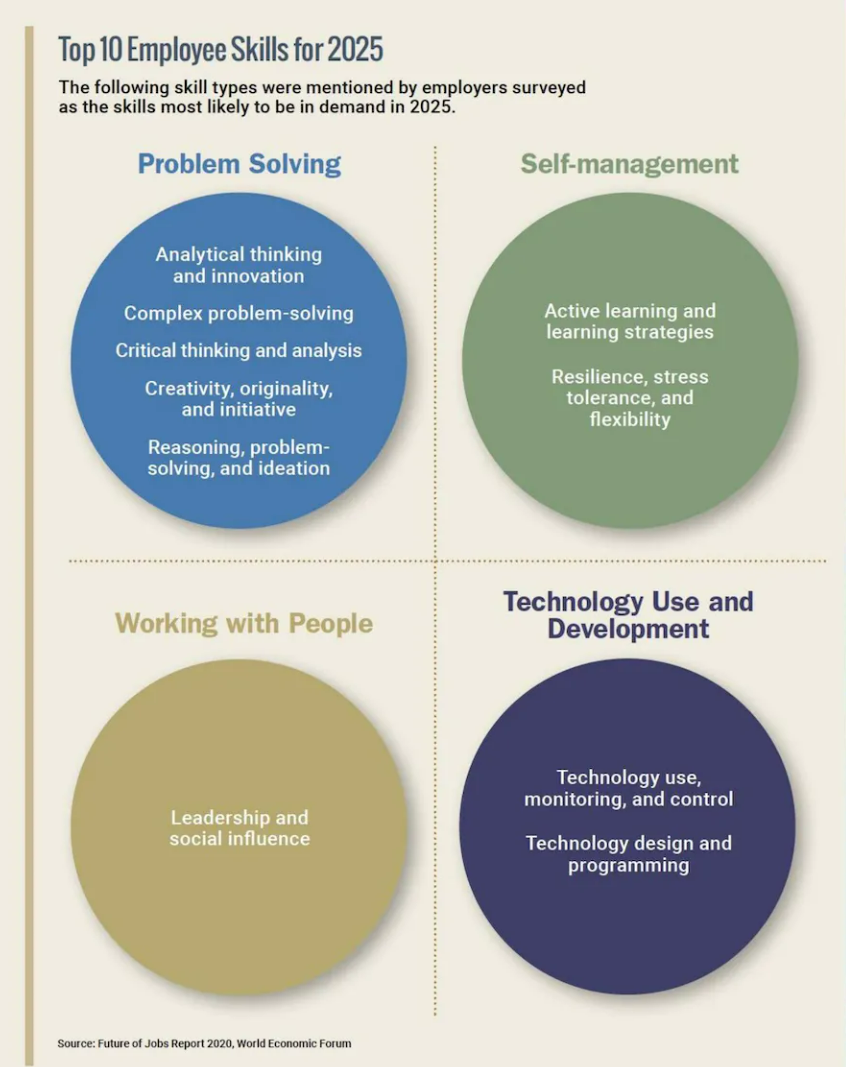
\includegraphics{assets/u6/Top Employee Skills 2025.png}

\end{figure}%

\emph{Source}: From ``Centre for Calling \& Career Development,'' by
Trinity Western University. n.d.,
(\href{https://www.twu.ca/academics/academic-professional-support/centre-calling-career-development}{Centre
for Calling \& Career Development \textbar{} Trinity Western
University}).

\begin{itemize}
\tightlist
\item
  \textbf{Write}: What competencies do you see that relate to social
  learning and digital skills? As this course aims to prepare you for
  the technology skills that are needed in this digital age, we also
  want to encourage you to develop personal and professional learning
  networks to discover and share knowledge, collaborate with others, and
  become engaged digital global citizens.
\end{itemize}

Consider the following questions:

\begin{itemize}
\tightlist
\item
  What skills and competencies do you want to practice to be successful
  in your future career?
\item
  How does collaborative learning and sharing your learning contribute
  to your learning journey?
\end{itemize}

Feel free to share your thoughts in your Obsidian journal, Discourse, or
your WordPress blog.

\end{tcolorbox}

\section{Digital Practices in the
Workplace}\label{digital-practices-in-the-workplace}

Let's fast forward to a time when you graduate from Trinity---fully
equipped with the knowledge, skills, character, and creativity to make a
lasting impact in the world. What digital skills will you have to
prepare you for your future career? In this topic we consider how
changes in technology have and will continue to impact digital practices
in the workplace. Pause and consider the following questions:

\begin{itemize}
\tightlist
\item
  How do professionals in your field of interest network online?
\item
  How has technology changed business practices in your field of
  interest or career?
\item
  What are the implications for learning and skills development in your
  future career precipitated by changes in digital technology?
\end{itemize}

\subsection{Activity: The Future of
Work}\label{activity-the-future-of-work}

\begin{tcolorbox}[enhanced jigsaw, toprule=.15mm, colback=white, colframe=quarto-callout-note-color-frame, bottomtitle=1mm, leftrule=.75mm, coltitle=black, titlerule=0mm, rightrule=.15mm, colbacktitle=quarto-callout-note-color!10!white, left=2mm, title={Learning Activity}, opacitybacktitle=0.6, opacityback=0, breakable, toptitle=1mm, arc=.35mm, bottomrule=.15mm]

In the following short video, \href{http://eduvation.ca/bio/}{Ken
Steele} from Eduvation speculates about the future of the labour market
and the value of higher education in a digital age.

\begin{itemize}
\tightlist
\item
  \textbf{Watch}:
  \href{https://www.youtube.com/watch?v=iY4UhfQefdU}{Higher Ed Trends:
  Student Career Anxiety and the Future of Work} (2015)
\end{itemize}

\href{https://www.youtube.com/watch?v=iY4UhfQefdU}{Watch: \emph{Higher
Ed Trends: Student Career Anxiety and the Future of Work}}

\url{https://www.youtube-nocookie.com/embed/iY4UhfQefdU}

What do you think? Share your thoughts by posting a comment on
Discourse, for example:

\begin{itemize}
\tightlist
\item
  Higher education is valuable because \ldots{}
\item
  In a digital age \ldots{}
\item
  I am confident that \ldots{}
\item
  I am concerned about \ldots{}
\end{itemize}

\end{tcolorbox}

\subsection*{Technology and Change}\label{technology-and-change}
\addcontentsline{toc}{subsection}{Technology and Change}

Throughout history there are technologies that have influenced change in
society. Consider, for example, the invention of the steam engine and
its contribution to the Industrial Revolution. In more recent times, the
advent of digital photography displaced Kodachrome (at one time, the
market leader in colour film sales) which ceased production in 2009.

\subsection{Activity: Newspaper and Music Industry in a Digital
Age}\label{activity-newspaper-and-music-industry-in-a-digital-age}

\begin{tcolorbox}[enhanced jigsaw, toprule=.15mm, colback=white, colframe=quarto-callout-note-color-frame, bottomtitle=1mm, leftrule=.75mm, coltitle=black, titlerule=0mm, rightrule=.15mm, colbacktitle=quarto-callout-note-color!10!white, left=2mm, title={Learning Activity}, opacitybacktitle=0.6, opacityback=0, breakable, toptitle=1mm, arc=.35mm, bottomrule=.15mm]

The readings that follow take a retrospective look at the impact of the
internet on the newspaper and music industries.

\begin{itemize}
\tightlist
\item
  \textbf{Read}:

  \begin{itemize}
  \tightlist
  \item
    \href{https://www.forbes.com/sites/joshwilson/2022/09/14/the-age-of-digital-music-executive-reacts-to-the-impact-of-digitalization-in-the-music-industry/?sh=1ca7f385537b}{The
    age of Digital; Music Executive Reacts to the Impact of
    Digitalization in the Music Industry} (2022)
  \item
    \href{https://medium.com/@kumarpriyanshu025/the-future-of-newspapers-in-the-digital-age-embracing-the-change-fe835bd8d52f}{The
    Future of Newspapers in the Digital Age: Embracing the Change!}
    (2023)
  \end{itemize}
\item
  \textbf{Annotate}: Add or reply to annotations using
  \href{https://web.hypothes.is/}{Hypothes.is}, sharing personal
  insights and experiences. Remember to tag your posts using the course
  code: LDRS101.
\end{itemize}

\end{tcolorbox}

\subsection{Activity: Impact of Digital Technology on
Business}\label{activity-impact-of-digital-technology-on-business}

\begin{tcolorbox}[enhanced jigsaw, toprule=.15mm, colback=white, colframe=quarto-callout-note-color-frame, bottomtitle=1mm, leftrule=.75mm, coltitle=black, titlerule=0mm, rightrule=.15mm, colbacktitle=quarto-callout-note-color!10!white, left=2mm, title={Learning Activity}, opacitybacktitle=0.6, opacityback=0, breakable, toptitle=1mm, arc=.35mm, bottomrule=.15mm]

\begin{itemize}
\tightlist
\item
  \textbf{Discuss}: Join the Discourse discussion on the impact of
  digital technology on business:
\item
  Choose any business or work environment (for example, your current
  career or future career).
\item
  Think about examples of how digital technology has had an impact on
  your chosen business over the last 30 years.
\item
  State your business or work environment and share a practical example
  of how digital technology has influenced change in your chosen area:
\item
  Has the example contributed to a fundamental change in the way things
  were done, or is this a minor change?
\item
  Do you anticipate significant changes in your industry as a result of
  digital technology in the future? Provide an example.
\end{itemize}

Like, share, and reply to posts. These are forms of engagement and a
contribution to your online learning identity. Remember to tag your
posts using the course code: LDRS101.

\end{tcolorbox}

\subsection*{Artificial Intelligence}\label{artificial-intelligence}
\addcontentsline{toc}{subsection}{Artificial Intelligence}

Artificial intelligence (AI) is predicted to have a significant impact
on society and business. Examples include autonomous cars, computers
understanding human speech, and machine learning. Consider for instance
that computer chess games available for commercial desktop machines have
the ability to beat accomplished chess players including grand masters.
And of course, Chat GPT.

In this section we introduce a few interesting examples of artificial
intelligence to provide a sense of how sophisticated these technologies
are becoming.

First, let's define AI:

\begin{quote}
The theory and development of computer systems able to perform tasks
normally requiring human intelligence, such as visual perception, speech
recognition, decision-making, and translation between languages. (Oxford
Reference, n.d.)
\end{quote}

\begin{quote}
The capacity of a computer, robot, programmed device, or software
application to perform operations and tasks analogous to learning and
decision making in humans, such as speech recognition or question
answering. (Dictionary.com, 2024)
\end{quote}

What is your experience with AI? Have you used an AI tool such as
Grammerly or ChatGPT? How has this technology affected you as a student,
and what effect do you think it has had or will have on your chosen
profession?

In the next activity, we'll explore some of these questions and
concerns.

\subsection{Activity: How Can I Use AI as a
Student?}\label{activity-how-can-i-use-ai-as-a-student}

\begin{tcolorbox}[enhanced jigsaw, toprule=.15mm, colback=white, colframe=quarto-callout-note-color-frame, bottomtitle=1mm, leftrule=.75mm, coltitle=black, titlerule=0mm, rightrule=.15mm, colbacktitle=quarto-callout-note-color!10!white, left=2mm, title={Learning Activity}, opacitybacktitle=0.6, opacityback=0, breakable, toptitle=1mm, arc=.35mm, bottomrule=.15mm]

\begin{itemize}
\tightlist
\item
  \textbf{Read}: First, do a quick search online for AI tools for
  university students. Examples:

  \begin{itemize}
  \tightlist
  \item
    \href{https://www.timeshighereducation.com/student/advice/how-can-ai-be-used-university-students}{How
    can AI be Used by University Students?} (2023)
  \item
    \href{https://mystudylife.com/10-best-ai-tools-to-help-students-learn-faster/}{10
    Best AI Tools for Homework and Studying in 2024} (2023)
  \end{itemize}
\end{itemize}

Intrigued? Do you find any tech tools that would be useful in
understanding course topics, studying, generating flashcards,
transcribing lectures and voice notes, correcting grammar, writing an
essay, creating a slideshow presentation, drafting a forum discussion
post, and so on?

Do any of these capabilities concern you? Do you think they concern your
professors or fellow students?

Review TWU's policy on
\href{https://www.twu.ca/about-us/policies-guidelines/university-policies/academic-misconduct-fraud}{Academic
Misconduct \& Fraud} (n.d.-a). Is it academic fraud if you use Chat GPT
to complete assignments?

Prote: italicize linked titles in paras above and below

Search online for key words related to this issue, such as ``university
concern policy artificial intelligence'' and you will find numerous
articles on the use of AI in universities, as well as emerging policies.
The University of Toronto's guidelines and FAQ for
\href{https://www.viceprovostundergrad.utoronto.ca/strategic-priorities/digital-learning/special-initiative-artificial-intelligence/}{ChatGPT
and Generative AI in the Classroom} (2024) are one such example.

Here are some guidelines you may receive from your instructors at TWU:

\begin{itemize}
\tightlist
\item
  Students are encouraged to make use of technology including generative
  artificial intelligence tools to contribute to their understanding of
  course materials. Students must submit as an appendix with their
  assignments any content produced by an artificial intelligence tool,
  and the prompt used to generate the content.
\item
  Any content produced by an artificial intelligence tool must be cited
  appropriately. Many organizations that publish standard citation
  formats now provide information on citing generative AI (e.g.,
  \href{https://style.mla.org/citing-generative-ai/}{MLA Style Center}).
\item
  Students may use artificial intelligence tools for creating an outline
  for an assignment but the final submitted assignment must be original
  work produced by the individual student alone.
\item
  Students may not use artificial intelligence tools for taking tests,
  writing research papers, creating computer code, or completing major
  course assignments. However, these tools may be useful when gathering
  information across sources and assimilating it for understanding.
\end{itemize}

If you have any question about the use of AI applications for course
work, please speak with your instructor.

\begin{itemize}
\tightlist
\item
  \textbf{Watch}: \href{https://www.youtube.com/watch?v=hJP5GqnTrNo}{How
  AI Could Save (Not Destroy) Education} (2023)
\end{itemize}

\url{https://www.youtube-nocookie.com/embed/hJP5GqnTrNo}

Here is one more article that discusses the pros and cons of English
learners using AI in their studies:

\begin{itemize}
\tightlist
\item
  \href{https://www.researchgate.net/publication/374483468_Perspectives_of_the_Use_of_ChatGPT_as_a_Tool_for_Online_Education_of_English}{\emph{Perspectives
  of the Use of ChatGPT as a Tool for Online Education of English}}
  (2023)
\end{itemize}

\end{tcolorbox}

\subsection{Activity: How to Identify AI Generated
Text}\label{activity-how-to-identify-ai-generated-text}

\begin{tcolorbox}[enhanced jigsaw, toprule=.15mm, colback=white, colframe=quarto-callout-note-color-frame, bottomtitle=1mm, leftrule=.75mm, coltitle=black, titlerule=0mm, rightrule=.15mm, colbacktitle=quarto-callout-note-color!10!white, left=2mm, title={Learning Activity}, opacitybacktitle=0.6, opacityback=0, breakable, toptitle=1mm, arc=.35mm, bottomrule=.15mm]

Explore the infographic below by Ryan Morrison.

Consider trying out ChatGPT to see if you can spot the ways to identify
AI generated writing.

\begin{itemize}
\tightlist
\item
  \textbf{Watch}:
  \href{https://www.youtube.com/watch?v=zuvN8_6QIKk}{Plagiarizing
  ChatGPT - Is it Illegal?} (2022)
\end{itemize}

\url{https://www.youtube-nocookie.com/embed/zuvN8_6QIKk}

\begin{itemize}
\tightlist
\item
  \textbf{Read}: Optional resource:
  \href{https://www.iesalc.unesco.org/wp-content/uploads/2023/04/ChatGPT-and-Artificial-Intelligence-in-higher-education-Quick-Start-guide_EN_FINAL.pdf}{ChatGPT
  and Artificial Intelligence in Higher Education: Quick Start Guide}.
  (2023)
\end{itemize}

\end{tcolorbox}

\subsection*{Jobs and Automation}\label{jobs-and-automation}
\addcontentsline{toc}{subsection}{Jobs and Automation}

In this section we consider the impact of automation on the future job
market and the implications for education and training. Consider:

\begin{itemize}
\tightlist
\item
  Will robots replace humans?
\item
  What jobs are most at risk of being replaced by robots?
\item
  What are the implications for learning in a digital age?
\end{itemize}

\subsection{Activity: Impact of Automation and AI in the
Workplace}\label{activity-impact-of-automation-and-ai-in-the-workplace}

\begin{tcolorbox}[enhanced jigsaw, toprule=.15mm, colback=white, colframe=quarto-callout-note-color-frame, bottomtitle=1mm, leftrule=.75mm, coltitle=black, titlerule=0mm, rightrule=.15mm, colbacktitle=quarto-callout-note-color!10!white, left=2mm, title={Learning Activity}, opacitybacktitle=0.6, opacityback=0, breakable, toptitle=1mm, arc=.35mm, bottomrule=.15mm]

\begin{itemize}
\tightlist
\item
  \textbf{Read:}
  \href{https://www.youtube.com/watch?v=7Pq-S557XQU}{\emph{Collaborative
  Intelligence: Humans and AI are Joining Forces}} (2018).
\item
  \textbf{Watch}:
  \href{https://www.youtube.com/watch?v=7Pq-S557XQU}{Humans Need Not
  Apply} (2014)
\end{itemize}

\url{https://www.youtube-nocookie.com/embed/7Pq-S557XQU}

Consider your chosen field of study. How can AI benefit your industry?
Are there any concerns regarding how AI might be used?

\end{tcolorbox}

\subsection{Activity: The Price of AI}\label{activity-the-price-of-ai}

\begin{tcolorbox}[enhanced jigsaw, toprule=.15mm, colback=white, colframe=quarto-callout-note-color-frame, bottomtitle=1mm, leftrule=.75mm, coltitle=black, titlerule=0mm, rightrule=.15mm, colbacktitle=quarto-callout-note-color!10!white, left=2mm, title={Learning Activity}, opacitybacktitle=0.6, opacityback=0, breakable, toptitle=1mm, arc=.35mm, bottomrule=.15mm]

In this topic we've explored AI---its possibilities for study and
careers, and some concerns about using AI. This activity focuses on how
AI moderates harmful content. How does AI know what is harmful? Since AI
tools are built on all kinds of information, including harmful and
hateful content, how is this content identified?

AI systems require lots of work from humans to function correctly. A
2023 report from Time magazine showed that people in Kenya were paid
poverty wages to build a safety system into ChatGPT (Perrigo, 2023).
Since the platform was fed data from various places sometimes it would
make racist or abusive remarks. To build a safeguard into the system
workers were exposed to vile and offensive web content in order to tag
it so that the platform could eventually recognize offensive speech on
its own. A large portion of this content was very traumatic, and workers
interviewed said they were mentally scarred from the work.

\begin{itemize}
\tightlist
\item
  \textbf{Read:}

  \begin{itemize}
  \tightlist
  \item
    \href{https://time.com/6247678/openai-chatgpt-kenya-workers/}{OpenAI
    Used Kenyan Workers on Less Than \$2 Per Hour to Make ChatGPT Less
    Toxic} (2023)
  \item
    \href{https://time.com/6147458/facebook-africa-content-moderation-employee-treatment/}{Inside
    Facebook's African Sweatshop} (2022)
  \end{itemize}
\item
  \textbf{Watch}:
  \href{https://www.youtube.com/watch?v=ug_p2wHhla0}{Doing Grueling Work
  for an AI: Data Labeling} (2023)
\end{itemize}

\url{https://www.youtube-nocookie.com/embed/ug_p2wHhla0}

\begin{itemize}
\tightlist
\item
  \textbf{Questions to Consider:}

  \begin{itemize}
  \tightlist
  \item
    Is it ethical to submit Kenyan workers to trauma in order to
    sanitize ChatGPT for other users?
  \item
    What other solutions are there for training AI to moderate content?
  \end{itemize}
\item
  \textbf{Share} your thoughts on AI by posting a comment on Discourse,
  for example:

  \begin{itemize}
  \tightlist
  \item
    AI will \ldots{}
  \item
    I was surprised that AI \ldots{}
  \item
    In {[}insert business{]} AI will \ldots{}
  \end{itemize}
\end{itemize}

\end{tcolorbox}

\section{Societal Issues and the
Internet}\label{societal-issues-and-the-internet}

In this next topic we introduce a number of societal issues and
problematic online behaviours that have emerged in the digital world.
Our list is not comprehensive and does not provide a thorough
examination of the issues. Here, we encourage you to choose an issue for
further investigation.

Choose one societal issue or antisocial behaviour associated with the
internet that you would like to investigate further, and publish as an
editorial in your course blog. You will base your focus on your reading
of open access resources you find online. Your blog post will also help
you build your online identity.

\begin{itemize}
\tightlist
\item
  Website tracking
\item
  Online impersonation
\item
  Internet trolling
\item
  Online harassment
\item
  Psychological issues
\item
  Net neutrality
\item
  Digital redlining
\item
  Diversity, equity and inclusion
\end{itemize}

\subsection{Activity: Problematic Online Behaviours---Key Terms
Quiz}\label{activity-problematic-online-behaviourskey-terms-quiz}

\begin{tcolorbox}[enhanced jigsaw, toprule=.15mm, colback=white, colframe=quarto-callout-note-color-frame, bottomtitle=1mm, leftrule=.75mm, coltitle=black, titlerule=0mm, rightrule=.15mm, colbacktitle=quarto-callout-note-color!10!white, left=2mm, title={Learning Activity}, opacitybacktitle=0.6, opacityback=0, breakable, toptitle=1mm, arc=.35mm, bottomrule=.15mm]

To test your knowledge of concepts associated with problematic
behaviours online, we provide a short orientation quiz below. Once you
have attempted your first answer, and in the event that you are not
familiar or not sure what the alternatives mean, click the options to
find out more about the concept.

How did you do? Have you encountered any of these behaviours online?
Share your thoughts by posting a comment on Discourse.

\end{tcolorbox}

\subsection*{Website Tracking}\label{website-tracking}
\addcontentsline{toc}{subsection}{Website Tracking}

Website tracking is the practice of collecting data about a user's
online activities when they visit websites or use web services. This
data is gathered primarily for marketing and analytical purposes,
allowing website owners, advertisers, and service providers to better
understand user behaviour, tailor their services, and deliver targeted
content and advertisements. Before we delve into the details of web
tracking, watch the video below.

\subsection{Activity: The True Cost of Free
Websites}\label{activity-the-true-cost-of-free-websites}

\begin{tcolorbox}[enhanced jigsaw, toprule=.15mm, colback=white, colframe=quarto-callout-note-color-frame, bottomtitle=1mm, leftrule=.75mm, coltitle=black, titlerule=0mm, rightrule=.15mm, colbacktitle=quarto-callout-note-color!10!white, left=2mm, title={Learning Activity}, opacitybacktitle=0.6, opacityback=0, breakable, toptitle=1mm, arc=.35mm, bottomrule=.15mm]

Watch this \emph{Matrix} parody, a comedy skit published by
CollegeHumour, depicting that if you are not paying for the service, you
are not the consumer but the product.

\begin{itemize}
\tightlist
\item
  \textbf{Watch}: \href{https://www.youtube.com/watch?v=5pFX2P7JLwA}{The
  Terrifying Cost of ``Free'' Websites} (2016)
\end{itemize}

\url{https://www.youtube-nocookie.com/embed/5pFX2P7JLwA}

\end{tcolorbox}

Were you surprised by any ideas presented in the video? Do you think
this is a valid and reliable source for the topic?

Next we will give an overview of how website tracking works, how your
data is used, and how you can protect yourself online.

\subsubsection*{How Does Website Tracking
Work?}\label{how-does-website-tracking-work}
\addcontentsline{toc}{subsubsection}{How Does Website Tracking Work?}

\textbf{Cookies}: Cookies are small text files that websites store on
your device. They contain information about your online activities such
as login credentials, preferences, and browsing history. Websites use
cookies to recognize and remember you when you return, and they can also
track your movements across the site.

\textbf{IP Address Tracking}: Every device connected to the internet has
a unique IP address. Websites can log and analyze these addresses to
determine a user's approximate location and to track their visits.

\textbf{Analytics Tools}: Many websites use analytics tools such as
Google Analytics to monitor user behaviour. These tools track which
pages you visit, how long you stay on each page, and how you arrived at
the website (e.g., through a search engine or a referral from another
site). This data helps website owners optimize their content and user
experience.

\textbf{Ad Trackers}: Advertisers and ad networks use various techniques
to track your online behaviour. They place cookies on your device, which
allows them to follow your movements across multiple websites. This data
is used to deliver personalized ads based on your interests and browsing
history.

\textbf{Social Media Widgets}: Social media buttons and widgets on
websites can track your activity, even if you don't click them. They
often use this information to build a profile of your interests and
habits.

\textbf{Fingerprinting}: Fingerprinting is a technique that collects
data about your device and browser configuration such as your screen
resolution, installed fonts, and plugins. This information can be used
to create a unique identifier for your device and track your online
activities.

\textbf{Location Data}: Many websites request access to your device's
location information. This can be used to provide location-based
services, but it also allows websites to track your physical movements.

\textbf{Data Brokers}: Your data may be collected, aggregated, and sold
to data brokers who build detailed profiles about individuals. These
profiles can include your demographic information, interests, and online
behaviour.

\subsubsection*{How is my Data Used When I use the
Internet?}\label{how-is-my-data-used-when-i-use-the-internet}
\addcontentsline{toc}{subsubsection}{How is my Data Used When I use the
Internet?}

\textbf{Personalization}: Websites and online services use the data they
collect to personalize your experience; for example, they may recommend
products, content, or services based on your browsing history and
preferences.

\textbf{Targeted Advertising}: Advertisers use your data to show you ads
that are more likely to be relevant to your interests. This is why you
might see ads for products you've recently searched for online.

\textbf{Analytics and Optimization}: Website owners use tracking data to
improve their websites and services, making them more user friendly and
effective.

\textbf{Market Research}: Aggregated user data is often used for market
research and to identify trends and consumer preferences.

\textbf{Data Profiling}: Your data may be used to build detailed
profiles about you. These profiles can be used for a variety of purposes
including credit scoring, job recruiting, and targeted marketing.

\textbf{Security and Fraud Prevention}: Tracking data can also be used
for security purposes, helping to detect and prevent fraudulent
activities.

\subsubsection*{What are the Privacy
Concerns?}\label{what-are-the-privacy-concerns}
\addcontentsline{toc}{subsubsection}{What are the Privacy Concerns?}

Privacy concerns regarding website tracking primarily revolve around the
collection and use of personal data without the explicit consent of
users. Here are some key privacy concerns and ways in which users can
protect themselves from tracking:

\textbf{Invasion of Privacy}: Website tracking can create a detailed
profile of an individual's online behaviour, which may include sensitive
information such as health concerns, financial status, or personal
interests. This can be seen as an invasion of privacy.

\textbf{Data Breaches}: There is an increased risk of data breaches when
your data is collected and stored by multiple parties. If a hacker gains
access to a company's database that stores user data, your personal
information may be exposed.

\textbf{Targeted Advertising}: While some users appreciate personalized
ads, others find them intrusive and a form of manipulation. The
extensive tracking of online behaviour allows advertisers to deliver
highly targeted ads, which can feel invasive.

\textbf{Third-Party Sharing}: Data collected by websites is often shared
with third-party companies, including data brokers and ad networks.
Users may not be aware of who has access to their data and how it's
used.

\subsubsection*{How can I Protect Myself From
Tracking?}\label{how-can-i-protect-myself-from-tracking}
\addcontentsline{toc}{subsubsection}{How can I Protect Myself From
Tracking?}

\textbf{Use Privacy-Focused Browsers}: Consider using web browsers that
prioritize user privacy, such as Mozilla Firefox or the Tor Browser.
These browsers often include built in tracking protection features.

\textbf{Browser Extensions}: Install browser extensions or add-ons such
as uBlock Origin, Privacy Badger, and HTTPS Everywhere, which can block
tracking cookies, scripts, and enhance your online security.

\textbf{Opt-Out Options}: Some websites and advertising networks provide
options to opt out of personalized ads. You can often find these
settings in the privacy sections of websites or through industry
specific opt-out platforms such as the Network Advertising Initiative
(NAI) or the Digital Advertising Alliance (DAA).

\textbf{Use a VPN}: A virtual private network (VPN) can hide your IP
address and encrypt your internet traffic, making it more challenging
for websites to track your location and online activities.

\textbf{Cookie Settings}: Adjust your browser's cookie settings to block
third-party cookies. You can choose to accept cookies only from visited
websites, which limits tracking across different sites.

\textbf{Use Private Browsing Modes}: Most browsers offer private or
incognito modes that don't store your browsing history or cookies. While
this doesn't provide complete anonymity, it limits tracking to a single
session.

\textbf{Search Engines}: Consider using privacy focused search engines
such as DuckDuckGo or Startpage, which do not track your search queries.

\textbf{Review App Permissions}: On mobile devices, review and restrict
the permissions granted to apps, including location access. Some apps
collect more data than necessary for their core functionality.

\textbf{Regularly Clear Cookies}: Periodically clear your browser's
cookies and browsing history to remove tracking data that has been
collected over time.

\textbf{Educate Yourself}: Stay informed about online privacy and data
protection practices. Understand the privacy policies of websites and
services you use and be cautious about sharing personal information
online.

\textbf{Consider VPNs and Encrypted Messaging}: For heightened privacy,
use end-to-end encrypted messaging apps such as Signal, and consider
using a reputable VPN service to protect your online communication.

It's important to note that while these steps can help reduce online
tracking they might not completely eliminate it. Achieving complete
anonymity on the internet is challenging, but these measures can
significantly enhance your online privacy and data security.
Additionally, privacy laws and regulations in your region may provide
you with rights and options for controlling how your data is collected
and used online.

\subsection{Activity: Website Tracking
Resources}\label{activity-website-tracking-resources}

\begin{tcolorbox}[enhanced jigsaw, toprule=.15mm, colback=white, colframe=quarto-callout-note-color-frame, bottomtitle=1mm, leftrule=.75mm, coltitle=black, titlerule=0mm, rightrule=.15mm, colbacktitle=quarto-callout-note-color!10!white, left=2mm, title={Learning Activity}, opacitybacktitle=0.6, opacityback=0, breakable, toptitle=1mm, arc=.35mm, bottomrule=.15mm]

\begin{itemize}
\tightlist
\item
  \textbf{Read}: Choose from the resources below to inform your views on
  website and data tracking:

  \begin{itemize}
  \tightlist
  \item
    \href{http://mediashift.org/2018/01/real-cost-free-internet/}{\emph{The
    Real Cost of the `Free' Internet}} (2018)
  \item
    \href{https://www.techdirt.com/2012/12/20/stop-saying-if-youre-not-paying-youre-product/}{\emph{Stop
    Saying `If You're not Paying, You're the Product'}} (2012)
  \item
    \href{https://link.springer.com/article/10.1007/s11528-021-00599-4}{\emph{Don't
    Be Evil: Should we use Google in Schools?}} (2021)
  \end{itemize}
\end{itemize}

Also review these resources on corporate sponsored research:

\begin{itemize}
\tightlist
\item
  \href{https://en.wikipedia.org/wiki/Funding_bias}{Funding Bias} (2024)
\item
  \href{https://trialsjournal.biomedcentral.com/articles/10.1186/1745-6215-13-146}{Sponsors'
  Participation in Conduct and Reporting of Industry Trials: A
  Descriptive Study} (2012)
\item
  \href{https://en.wikipedia.org/wiki/Ad_blocking}{Ad Blocking} (2024)
\end{itemize}

After viewing these resources, what do you think the cost of free
websites is? Do you use ad blocking software? Think about the reasons
for your choice.

\begin{itemize}
\tightlist
\item
  \textbf{Write}: Share your thoughts on Discourse or use Hypothes.is to
  annotate and share your comments.
\end{itemize}

\end{tcolorbox}

\subsection{Activity: Forum: Philanthropy and Corporate
Advertising}\label{activity-forum-philanthropy-and-corporate-advertising}

\begin{tcolorbox}[enhanced jigsaw, toprule=.15mm, colback=white, colframe=quarto-callout-note-color-frame, bottomtitle=1mm, leftrule=.75mm, coltitle=black, titlerule=0mm, rightrule=.15mm, colbacktitle=quarto-callout-note-color!10!white, left=2mm, title={Learning Activity}, opacitybacktitle=0.6, opacityback=0, breakable, toptitle=1mm, arc=.35mm, bottomrule=.15mm]

Next, let's explore and reflect on the relationship between corporate
commercial interests and digital citizenship for learning in a digital
age.

\begin{itemize}
\tightlist
\item
  \textbf{Read} the following case study:
\end{itemize}

The \href{https://oeru.org/}{OERu} is a charitable organization which
provides open online courses for free, using open educational resources
which any educational institution can adopt, modify, and reuse. There
are costs that must be covered to sustain the OERu; for example, the
assembly of open online courses, hosting of server and software
infrastructure, staff to coordinate and support the initiative, and so
on. The OERu does not generate any revenue from corporate services; for
example, it does not allow advertising on OERu course sites for a share
of advertising revenue. Moreover, the OERu does not sell or generate
revenue from personal data learners provide by using these free learning
services, therefore users are not the product of this service.

\begin{itemize}
\tightlist
\item
  \textbf{Discuss}: Join the discussion in Discourse on philanthropy and
  corporate advertising. The key question is how can nonprofit
  organizations sustain free educational services for those who can't
  afford traditional education provision?
\end{itemize}

Consider the following issues:

\begin{itemize}
\tightlist
\item
  As a learner, how would you feel if course materials included
  corporate advertising? If advertising were to be supported, how would
  you feel if OERu course sites required you to switch off any ad
  blockers before gaining access to the course materials?
\item
  Is it appropriate for publicly funded institutions and charities
  working in education to generate revenue from corporate advertising to
  support and sustain free online services? What are the risks and
  opportunities?
\item
  Should education institutions and educational charities accept
  significant corporate sponsorship in return for profiling proprietary
  products?
\item
  The OERu has recommended that learners use free blogging services to
  share their learning outputs. Many of these services carry
  advertising. How do you feel about using these services---being the
  product rather than the consumer? Would it be better for OERu to
  recommend that learners use a paid service without advertising? How
  would this impact on learners who do not have sufficient funds to
  afford a domain of their own?
\item
  Other?
\end{itemize}

Remember to tag your posts using the course code: LDRS101

\end{tcolorbox}

\subsubsection*{Online Impersonation}\label{online-impersonation}
\addcontentsline{toc}{subsubsection}{Online Impersonation}

Impersonation online refers to the act of creating an online presence in
someone else's name. This is potentially a complex issue as some social
media sites permit parody accounts or accounts that are intended to
represent real individuals. It is not necessarily illegal to impersonate
someone per se, for example in comedy, but online impersonation is a
growing problem. Many social media sites have anti-impersonation
policies, but this is not sufficient guarantee or protection against the
risks of online impersonation.

\subsection{Activity: Identify the
Imposter!}\label{activity-identify-the-imposter}

\begin{tcolorbox}[enhanced jigsaw, toprule=.15mm, colback=white, colframe=quarto-callout-note-color-frame, bottomtitle=1mm, leftrule=.75mm, coltitle=black, titlerule=0mm, rightrule=.15mm, colbacktitle=quarto-callout-note-color!10!white, left=2mm, title={Learning Activity}, opacitybacktitle=0.6, opacityback=0, breakable, toptitle=1mm, arc=.35mm, bottomrule=.15mm]

\begin{itemize}
\tightlist
\item
  \textbf{View}: Visit the profile page of following X (Twitter)
  accounts:

  \begin{itemize}
  \tightlist
  \item
    \href{https://twitter.com/NelsonMandela}{Nelson Mandela}
  \item
    \href{https://twitter.com/notzuckerberg}{Mark Zuckerburg}
  \item
    \href{https://twitter.com/ElonMuskAOC}{Elon Musk}
  \item
    \href{https://twitter.com/DarthVader}{Darth Vader}
  \end{itemize}
\end{itemize}

Clearly these social media accounts are not the ``real'' people. In one
case it's a foundation promoting the legacy of Nelson Mandela, the next
two examples are parody accounts of two tech giants, and the last
example is, well, Darth Vader!

\begin{itemize}
\tightlist
\item
  \textbf{Read} the following articles on the social media response to
  impersonation:

  \begin{itemize}
  \tightlist
  \item
    \href{https://help.twitter.com/en/rules-and-policies/x-impersonation-and-deceptive-identities-policy}{\emph{Misleading
    and Deceptive Identities Policy (X)}} (2023)
  \item
    \href{https://www.facebook.com/help/174210519303259}{\emph{How to
    Report a Facebook Account or Page That's Pretending to be me or
    Someone Else?}} (n.d.)
  \item
    \href{https://saferinternet.org.uk/blog/reporting-impersonation-on-social-media}{\emph{Reporting
    Impersonation on Social Media}} (2016)
  \end{itemize}
\end{itemize}

Have you seen a fake account on social media? What clues did you have
that it was not real?

\end{tcolorbox}

\begin{tcolorbox}[enhanced jigsaw, toprule=.15mm, colback=white, colframe=quarto-callout-note-color-frame, arc=.35mm, opacityback=0, breakable, rightrule=.15mm, bottomrule=.15mm, leftrule=.75mm, left=2mm]

\textbf{\emph{Note:}} If interested, search on X for some parody
accounts. Some can be quite entertaining, but you might notice that
other accounts simply mock the person they are parodying. Would you
create a parody account in order to ridicule someone---perhaps a
political view you don't agree with? What should our response be to such
messages on social media? How can we promote inclusive digital
communities which embody a sense of belonging, connection, and Christian
hospitality?

\end{tcolorbox}

\subsection{Activity: How to Spot a
Scammer}\label{activity-how-to-spot-a-scammer}

\begin{tcolorbox}[enhanced jigsaw, toprule=.15mm, colback=white, colframe=quarto-callout-note-color-frame, bottomtitle=1mm, leftrule=.75mm, coltitle=black, titlerule=0mm, rightrule=.15mm, colbacktitle=quarto-callout-note-color!10!white, left=2mm, title={Learning Activity}, opacitybacktitle=0.6, opacityback=0, breakable, toptitle=1mm, arc=.35mm, bottomrule=.15mm]

\begin{itemize}
\tightlist
\item
  \textbf{Watch}: Check out these two videos that share signs to help
  you identify online impersonation.

  \begin{itemize}
  \tightlist
  \item
    \href{https://www.youtube.com/watch?v=F57DE05FpgQ}{Watch out for
    Scammers Using Fake Instagram Profiles} (2023)
  \end{itemize}
\end{itemize}

\url{https://www.youtube-nocookie.com/embed/F57DE05FpgQ?si=Pq7GlHGpNCbTG0xu}

\begin{itemize}
\tightlist
\item
  \href{https://www.youtube.com/watch?v=Ta6qq7wnpcA}{Cyber Sandra's
  Hacks - Social Media Impersonation} (2021)
\end{itemize}

\url{https://www.youtube-nocookie.com/embed/Ta6qq7wnpcA}

\end{tcolorbox}

\subsection{Activity: Case Study on
Catfishing}\label{activity-case-study-on-catfishing}

\begin{tcolorbox}[enhanced jigsaw, toprule=.15mm, colback=white, colframe=quarto-callout-note-color-frame, bottomtitle=1mm, leftrule=.75mm, coltitle=black, titlerule=0mm, rightrule=.15mm, colbacktitle=quarto-callout-note-color!10!white, left=2mm, title={Learning Activity}, opacitybacktitle=0.6, opacityback=0, breakable, toptitle=1mm, arc=.35mm, bottomrule=.15mm]

Catfishing is the deceptive practice of creating a fictional online
presence to lure somebody into a relationship, for example, a romance
scam.

Dr.~Alec Couros is Associate Professor of Information and Communication
Technologies at the University of Regina, Saskatchewan. Dr.~Couros has
experienced a number of scams where his personal photos have been used
to lure woman into an online romantic relationship for the purpose of
``borrowing'' or extorting money. Check out his experiences:

\begin{itemize}
\tightlist
\item
  \textbf{Read}:

  \begin{itemize}
  \tightlist
  \item
    \href{https://www.cbc.ca/radio/spark/380-phantom-traffic-jams-catfishing-scams-and-smart-speakers-1.4482967/your-photos-can-be-used-in-catfishing-romance-scams-1.4482985}{\emph{Your
    Photos can be Used in `Catfishing' Romance Scams}} (2018a)
  \item
    \href{http://educationaltechnology.ca/2393/}{\emph{Identity, Love,
    and Catfishing}} (2013)
  \item
    \href{http://educationaltechnology.ca/2466/}{\emph{Would the Real
    `Alec Couros' Please Stand Up}} (2014)
  \item
    Visit this website that reports online scams:
    \href{https://romancescam.com/}{ScamDigger Forum} (n.d.).
  \end{itemize}
\item
  \textbf{Watch}:

  \begin{itemize}
  \tightlist
  \item
    \href{https://www.youtube.com/watch?v=s6Q4U8DvJH8}{Watch: \emph{How
    to Detect a Facebook Scammer With Google Reverse Image Search}}
    (2014)
  \end{itemize}
\end{itemize}

\url{https://www.youtube-nocookie.com/embed/s6Q4U8DvJH8}

Optional reading: (expletive warning)

\begin{itemize}
\tightlist
\item
  \href{https://cogdogblog.com/2015/10/facebook-as-catfish-paradise-its-community-standards-wears-the-cone-of-shame/}{\emph{Facebook
  as Catfish Paradise: Its Community Standards Wears the Cone of Shame}}
  (2015)
\end{itemize}

Feel free to share personal reflections on the phenomenon of online
impersonation by posting a comment on Discourse.

\end{tcolorbox}

\subsection*{Internet Trolling}\label{internet-trolling}
\addcontentsline{toc}{subsection}{Internet Trolling}

\begin{quote}
Sometimes trolls live under bridges. But not everyone living under a
bridge is a troll. (Wikimedia Foundations, n.d.)
\end{quote}

It is estimated that that the internet has about 5.473 billion users,
almost half the population of the world (Tsvetkova, 2023). With the
growing number of internet and social media users we are witnessing an
increase in antisocial behaviour online.

In this section we explore the phenomenon of internet trolling and
strategies for managing disruptive online behaviour, taking the
communication context into account.

\begin{quote}
In slang, a troll is a person who posts deliberately offensive or
provocative messages online (such as in social media, a newsgroup, a
forum, a chat room, an online video game) or who performs similar
behaviors in real life. The methods and motivations of trolls can range
from benign to sadistic. These messages can be inflammatory, insincere,
digressive, extraneous, or off-topic, and may have the intent of
provoking others into displaying emotional responses, or manipulating
others' perception, thus acting as a bully or a provocateur. The
behavior is typically for the troll's amusement, or to achieve a
specific result such as disrupting a rival's online activities or
purposefully causing confusion or harm to others. (``Troll (Slang),''
2024)
\end{quote}

\subsection{Activity: Trolling in Social
Media}\label{activity-trolling-in-social-media}

\begin{tcolorbox}[enhanced jigsaw, toprule=.15mm, colback=white, colframe=quarto-callout-note-color-frame, bottomtitle=1mm, leftrule=.75mm, coltitle=black, titlerule=0mm, rightrule=.15mm, colbacktitle=quarto-callout-note-color!10!white, left=2mm, title={Learning Activity}, opacitybacktitle=0.6, opacityback=0, breakable, toptitle=1mm, arc=.35mm, bottomrule=.15mm]

\begin{itemize}
\tightlist
\item
  \textbf{Quiz}: Take the \href{https://spotthetroll.org/}{Spot the
  Troll} quiz (n.d.), which uses images of real social media content.
  How did you do? Did some of the profiles surprise you? Have you
  encountered these types of profiles on social media?
\item
  \textbf{Read}: As you read the following, pay particular attention to
  strategies for dealing with trolling behaviour.

  \begin{itemize}
  \tightlist
  \item
    \href{https://en.wikipedia.org/wiki/Troll_(slang)\%7Btarget=\%22_blank\%22\%7D}{Troll
    (Slang)} (2024)
  \item
    \href{https://meta.wikimedia.org/wiki/What_is_a_troll}{What is a
    Troll?} (n.d.)
  \item
    \href{https://www.lifewire.com/what-is-internet-trolling-3485891}{Internet
    Trolling: How do you Spot a Real Troll?} (2024)
  \end{itemize}
\item
  \textbf{Watch}:

  \begin{itemize}
  \tightlist
  \item
    \href{https://www.youtube.com/watch?v=5BQp3V_34BE}{The Secret
    Confessions of an Internet Troll} (2016)
  \end{itemize}
\end{itemize}

\url{https://www.youtube-nocookie.com/embed/5BQp3V_34BE}

\begin{itemize}
\tightlist
\item
  \textbf{Annotate}: Read the following articles and add or reply to
  annotations on Hypothes.is, focusing on how the research relates to
  your own online experience. Remember to tag your posts using the
  course code: LDRS101.

  \begin{itemize}
  \tightlist
  \item
    \href{https://theconversation.com/dont-feed-the-trolls-really-is-good-advice-heres-the-evidence-63657}{`Don't
    Feed the Trolls' Really is Good Advice -- Here's the Evidence}
    (2016)
  \item
    \href{https://theconversation.com/how-empathy-can-make-or-break-a-troll-80680}{How
    Empathy can Make or Break a Troll} (2017)
  \end{itemize}
\end{itemize}

After viewing the resources, how can you spot trolls online? Share your
thoughts by posting a comment on Discourse.

\end{tcolorbox}

\subsection*{Online Harassment}\label{online-harassment}
\addcontentsline{toc}{subsection}{Online Harassment}

\begin{quote}
41 \% of Americans have been personally subjected to harassing behavior
online, and an even larger share (66 \%) has witnessed these behaviors
directed at others (Duggan, 2017).
\end{quote}

Many of us associate online harassment with extreme cases such as
cyberbullying and teenage suicide, or cyberstalking leading to physical
sexual harassment. Notwithstanding the seriousness of these offences,
antisocial behaviours associated with other forms of online harassment
are more pervasive than most people realize.

In this section, we will review research on the state of online
harassment and consider how leading social media sites attempt to manage
the challenge.

\subsection{Activity: The State of Online
Harassment}\label{activity-the-state-of-online-harassment}

\begin{tcolorbox}[enhanced jigsaw, toprule=.15mm, colback=white, colframe=quarto-callout-note-color-frame, bottomtitle=1mm, leftrule=.75mm, coltitle=black, titlerule=0mm, rightrule=.15mm, colbacktitle=quarto-callout-note-color!10!white, left=2mm, title={Learning Activity}, opacitybacktitle=0.6, opacityback=0, breakable, toptitle=1mm, arc=.35mm, bottomrule=.15mm]

\begin{itemize}
\tightlist
\item
  \textbf{Read} the following research reports on online harassment.

  \begin{itemize}
  \tightlist
  \item
    \emph{\href{https://www.pewresearch.org/internet/2014/10/22/online-harassment/}{Online
    Harassment}} (2017). (Note that this is an 8-page report; click
    through to read it all.)
  \item
    \href{https://www.pewresearch.org/short-reads/2021/01/13/qa-what-weve-learned-about-online-harassment/}{\emph{Q\&A:
    What We've Learned About Online Harassment}} (2021)
  \end{itemize}
\end{itemize}

Note in particular the finding that those ``who have ever experienced
more severe forms of harassment -- such as physical threats, stalking,
sexual harassment or sustained harassment -- or multiple forms of
harassing behaviors online have both risen substantially in the past
three years. This is not the pattern we saw in prior surveys. There has
been a markedly steeper rise in these measures since 2017, compared with
the change between our 2014 and 2017 studies'' (DeSilver, 2021).

\begin{itemize}
\tightlist
\item
  \textbf{Questions to Consider}:

  \begin{itemize}
  \tightlist
  \item
    What surprised you when reading these reports?
  \item
    Why have the forms of harassment become more severe?
  \item
    Have you or someone you know experienced some kind of online
    harassment?
  \end{itemize}
\item
  \textbf{Annotate}: Add or reply to annotations using Hypothes.is to
  share personal insights and experiences. Remember to tag your posts
  using the course code: LDRS101.
\end{itemize}

\end{tcolorbox}

\subsection{Activity: The Response From Social
Media}\label{activity-the-response-from-social-media}

\begin{tcolorbox}[enhanced jigsaw, toprule=.15mm, colback=white, colframe=quarto-callout-note-color-frame, bottomtitle=1mm, leftrule=.75mm, coltitle=black, titlerule=0mm, rightrule=.15mm, colbacktitle=quarto-callout-note-color!10!white, left=2mm, title={Learning Activity}, opacitybacktitle=0.6, opacityback=0, breakable, toptitle=1mm, arc=.35mm, bottomrule=.15mm]

\begin{itemize}
\tightlist
\item
  \textbf{Read}: Choose from the following resources about Facebook and
  X (Twitter) policies on online harassment, and responses to them.
\end{itemize}

\textbf{Suggested practices}

\begin{itemize}
\tightlist
\item
  \emph{\href{https://transparency.fb.com/en-gb/policies/community-standards/?source=https\%3A\%2F\%2Fwww.facebook.com\%2Fcommunitystandards\%2F}{Facebook
  Community Standards}} (n.d.)
\item
  \href{https://help.twitter.com/en/safety-and-security/cyber-bullying-and-online-abuse}{\emph{About
  Online Abuse}} (n.d.)
\end{itemize}

\textbf{Commentary}

\begin{itemize}
\tightlist
\item
  \href{https://money.cnn.com/2017/02/07/technology/twitter-combat-harassment-features/index.html?iid=EL}{\emph{Twitter
  Tries new Measures in Crackdown on Harassment}} (2017)
\item
  \href{https://www.forbes.com/sites/kalevleetaru/2017/02/06/using-digital-fingerprints-and-deep-learning-to-fight-online-harassment/?sh=49fc9bf06908}{\emph{Using
  Digital Fingerprints and Deep Learning to Fight Online Harassment}}
  (2017)
\item
  \href{https://www.theguardian.com/commentisfree/2017/may/22/facebook-get-things-wrong-but-safety-role-seriously}{\emph{At
  Facebook we get Things Wrong -- But we Take our Safety Role
  Seriously}} (2017). Please watch the
  \href{https://www.theguardian.com/news/video/2017/may/21/the-facebook-files-sex-violence-and-hate-speech-video-explainer}{\emph{video}}
  in this link!
\end{itemize}

\end{tcolorbox}

\subsection*{Psychological Issues}\label{psychological-issues}
\addcontentsline{toc}{subsection}{Psychological Issues}

The internet, social media, and mobile devices have introduced new
psychological issues. These include, for example, phantom ringing
syndrome, nomophobia, cybersickness, and internet addiction disorder.

In this section, we identify selected psychological issues that you may
choose to research further as you select a societal issue on which
you'll include comments on your blog.

\subsection{Activity: How Online Personas Are Redefining Human
Connection}\label{activity-how-online-personas-are-redefining-human-connection}

\begin{tcolorbox}[enhanced jigsaw, toprule=.15mm, colback=white, colframe=quarto-callout-note-color-frame, bottomtitle=1mm, leftrule=.75mm, coltitle=black, titlerule=0mm, rightrule=.15mm, colbacktitle=quarto-callout-note-color!10!white, left=2mm, title={Learning Activity}, opacitybacktitle=0.6, opacityback=0, breakable, toptitle=1mm, arc=.35mm, bottomrule=.15mm]

First, consider the following questions: - How does digital technology
change what we do? - How does digital technology change who we are? - Do
adolescents need to develop face-to-face communication skills in a
digital world? - \textbf{Watch}: Watch this fascinating TedTalk video: -
\href{https://www.youtube.com/watch?v=t7Xr3AsBEK4}{\emph{Connected, but
Alone?}} (2012) - \textbf{Write}: Jot down your thoughts in your
Reflective Journal (Obsidian).

\href{https://www.youtube.com/watch?v=t7Xr3AsBEK4}{Watch:
\emph{Connected, but alone? \textbar{} Sherry Turkle}}

\url{https://www.youtube-nocookie.com/embed/t7Xr3AsBEK4}

\begin{itemize}
\tightlist
\item
  \textbf{Read}: Finally, read the following article which summarizes a
  number of psychological disorders related to our use of digital
  technology:

  \begin{itemize}
  \tightlist
  \item
    \href{https://www.pcworld.com/article/448085/eight-new-mental-illnesses-brought-to-you-by-wait-for-it-the-internet.html}{\emph{Eight
    new Mental Illnesses Brought to you by the Internet}} (2013)
  \end{itemize}
\end{itemize}

Share your thoughts by posting a comment on Discourse, for example:

\begin{itemize}
\tightlist
\item
  I was surprised by \ldots{}
\item
  I think that \ldots{}
\item
  I don't agree that \ldots{}
\end{itemize}

\end{tcolorbox}

\subsection*{Net Neutrality}\label{net-neutrality}
\addcontentsline{toc}{subsection}{Net Neutrality}

\begin{quote}
The Web as I envisaged it, we have not seen it yet. The future is still
so much bigger than the past. (Tim Berners-Lee, 2009, as cited in
Medium, 2023)
\end{quote}

\begin{quote}
The World Wide Web was originally designed to provide universal access
to a large universe of documents. To achieve universal access it was
paramount to design the web as an open system without a central locus of
control. However, on the internet there are an increasing number of
``walled gardens'' that aim to control user's access to content and
services. In this section we explore the concept of net neutrality and
reflect on the risks associated with universal access to online
information.
\end{quote}

\textbf{\emph{Net neutrality}} is a critical concept in the realm of
internet policy and regulation. It revolves around the principle that
internet service providers (ISPs) should treat all data on the internet
equally. In other words, they should not discriminate against, or charge
differently based on user, content, website, application, or platform.
The primary goal of net neutrality is to ensure that the internet
remains an open and level playing field where all data and information
can be accessed and transmitted freely.

\subsubsection*{Arguments For Net
Neutrality}\label{arguments-for-net-neutrality}
\addcontentsline{toc}{subsubsection}{Arguments For Net Neutrality}

\begin{itemize}
\tightlist
\item
  \textbf{Preservation of open internet}: Net neutrality proponents
  argue that it is essential to maintain the open nature of the
  internet, where all content is equally accessible to users. This
  fosters innovation, competition, and free expression.
\item
  \textbf{Equal access}: Net neutrality ensures that users, regardless
  of their economic status, can access all online content without
  discrimination. It prevents ISPs from creating fast lanes for certain
  content, disadvantaging others.
\item
  \textbf{Innovation}: Without net neutrality, ISPs could prioritize
  certain services or websites, potentially stifling innovation by
  making it difficult for new, smaller players to compete on a level
  playing field.
\end{itemize}

\subsubsection*{Arguments Against Net
Neutrality}\label{arguments-against-net-neutrality}
\addcontentsline{toc}{subsubsection}{Arguments Against Net Neutrality}

\begin{itemize}
\tightlist
\item
  \textbf{Investment and infrastructure}: Opponents argue that without
  the ability to offer paid prioritization or tiered services, ISPs may
  have less incentive to invest in and improve network infrastructure,
  potentially hindering the growth of broadband services.
\item
  \textbf{Regulatory overreach}: Some argue that government intervention
  in net neutrality is unnecessary, and that market forces should
  determine how ISPs manage their networks. They fear that regulation
  could lead to unintended consequences such as the government
  controlling access to online content.
\item
  \textbf{Quality of service}: In certain cases, ISPs claim they need
  the flexibility to manage network traffic to provide a better quality
  of service for applications such as real-time video and gaming.
\end{itemize}

\subsubsection*{Key Concerns}\label{key-concerns}
\addcontentsline{toc}{subsubsection}{Key Concerns}

Concerns surrounding net neutrality involve potential discrimination, a
lack of competition, and the profound implications for free speech and
innovation. The absence of robust net neutrality principles could pave
the way for ISPs to exert unwarranted control. They might throttle or
obstruct access to specific websites, promote their own content, or levy
extra charges for particular online services.

At the same time there is a significant concern about government
overreach in this digital domain. The debate over how much the
government should regulate the internet is a hot topic, as it could
hamper innovation and limit the free sharing of information. Excessive
regulation could put the power to control or tamper with online content
in the hands of the government or regulators, potentially jeopardizing
our democratic values and our basic freedom of expression. Navigating
this tricky balance between rules and protecting our personal freedoms
is a key challenge in the digital era.

\subsubsection*{Canadian Context}\label{canadian-context}
\addcontentsline{toc}{subsubsection}{Canadian Context}

In Canada, the discussion on net neutrality is intertwined with the
debate over Bill C-10, also known as the Broadcasting Act. This bill,
introduced in 2021, aims to update Canada's broadcasting and
telecommunications regulations to account for the digital age. Critics
of Bill C-10 have expressed concerns that it could infringe on net
neutrality principles by giving more power to the Canadian
Radio-television and Telecommunications Commission (CRTC) to regulate
online content, potentially leading to restrictions on free expression
and innovation.

In addition to Bill C-10, another significant piece of legislation to
consider in the Canadian context is Bill C-18, which is also known as
the Online Streaming Act. This bill, introduced to the Canadian
Parliament, is designed to regulate online streaming services,
potentially affecting the content and accessibility of such platforms.
Critics argue that Bill C-18 could raise concerns related to net
neutrality by granting the government more authority over the content
available on streaming platforms and potentially infringing on free
expression and access to diverse content.

*** Questions to Consider ***

As you view the resources in the activity below, consider the following
questions:

\begin{itemize}
\tightlist
\item
  How does the principle of net neutrality impact the way you access and
  use the internet, and how might changes in net neutrality regulations
  affect your online experience?
\item
  What is the role of government and regulatory bodies, such as the CRTC
  in Canada, in ensuring a balance between net neutrality and the need
  to regulate online content and services?
\item
  What measures can be taken to ensure that government regulations,
  while addressing valid concerns, do not lead to the overreach of power
  and the erosion of fundamental rights such as free speech on the
  internet?
\item
  Can net neutrality coexist with the goal of ensuring high quality
  internet service and fostering investment in digital infrastructure,
  or are these objectives inherently in conflict?
\end{itemize}

Consider drawing a mind map such as the following to track your
understanding of the subject.

\begin{figure}

\caption{\label{fig-4540678705xff7936561a}Net Neutrality and Creative
Freedom Mind Map Illustration}

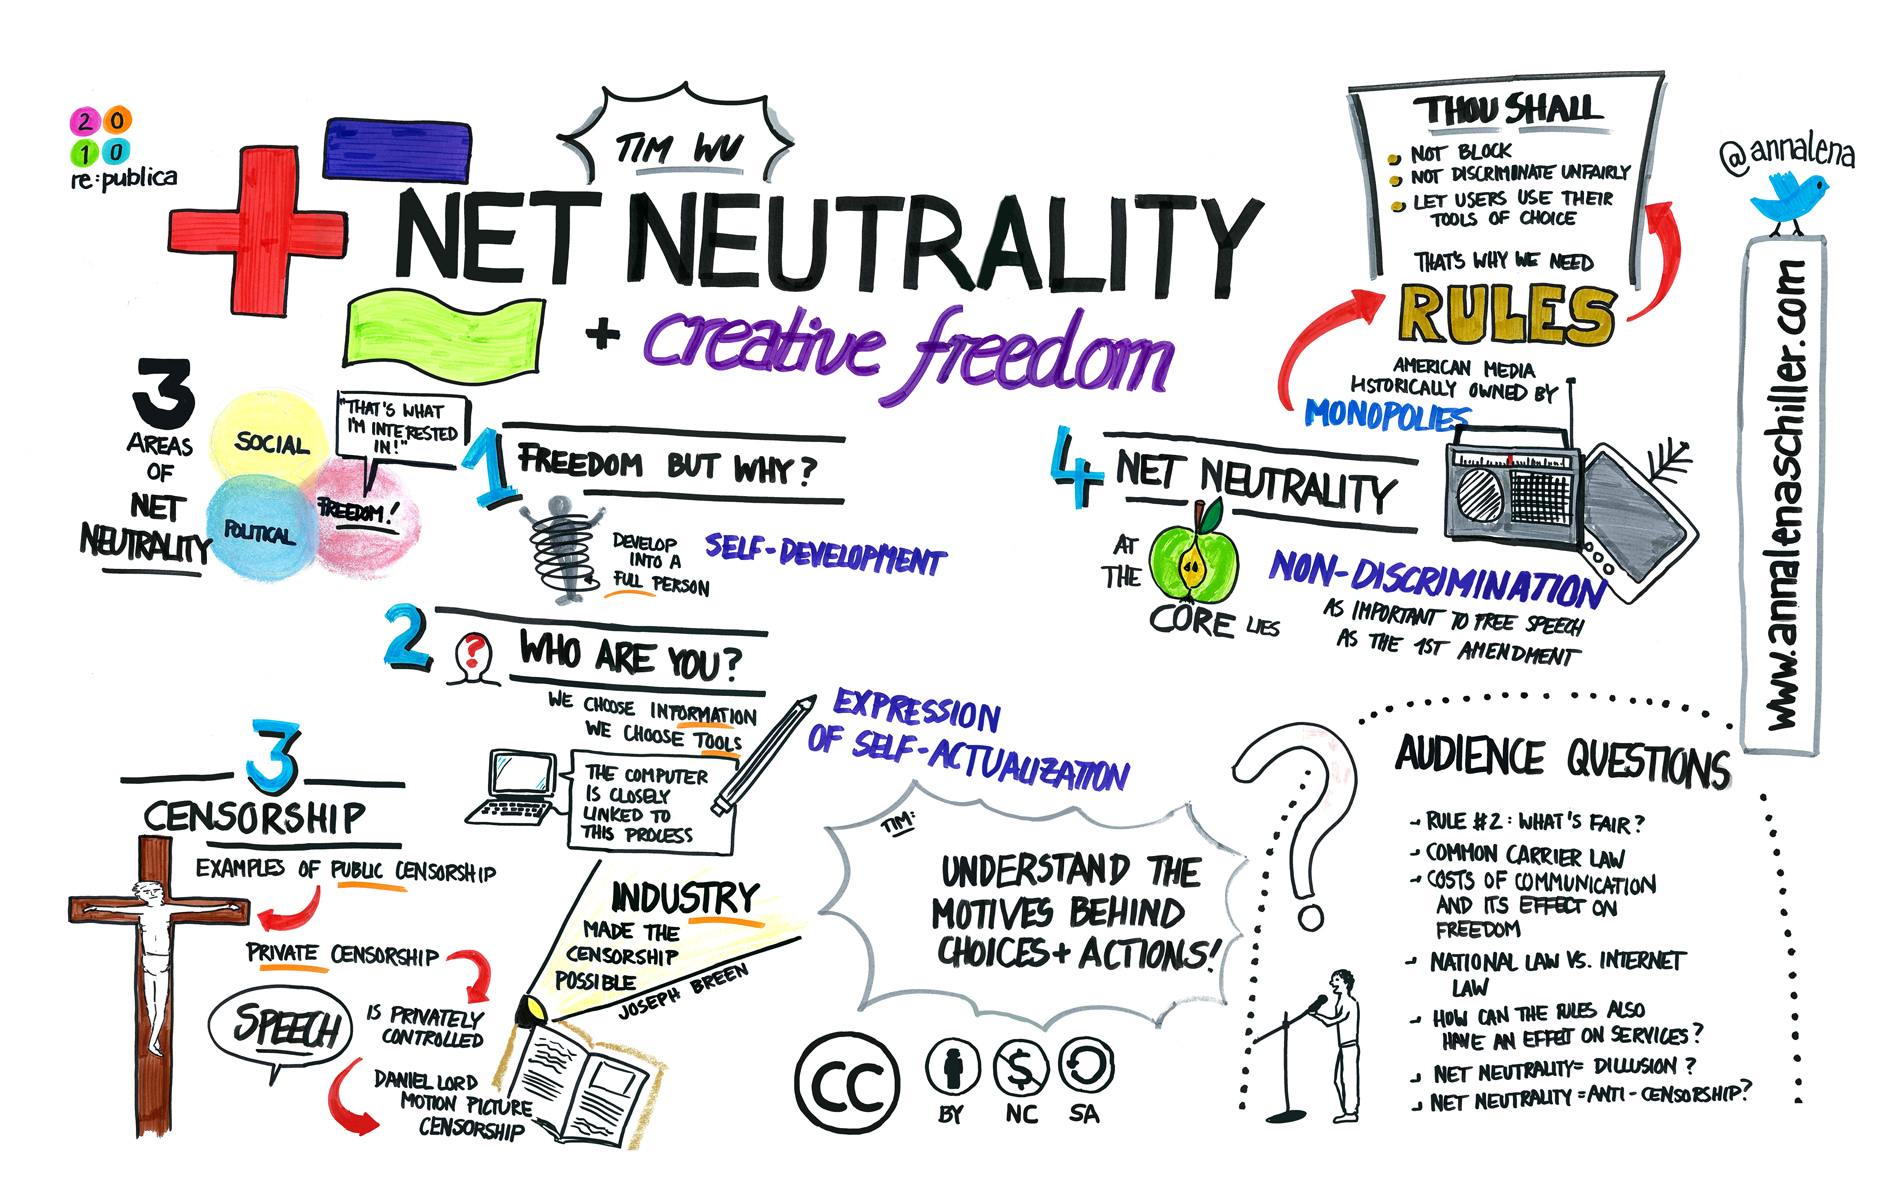
\includegraphics{assets/u6/net_neutrality_creative_freedom.jpg}

\end{figure}%

\begin{tcolorbox}[enhanced jigsaw, toprule=.15mm, colback=white, colframe=quarto-callout-note-color-frame, arc=.35mm, opacityback=0, breakable, rightrule=.15mm, bottomrule=.15mm, leftrule=.75mm, left=2mm]

\emph{Note}: From ``Net Neutrality and Creative Freedom: Tim Wu at
re:publica 2010,'' by A. L. Schiller, April 10, 2010, Flickr,
(https://flickr.com/photos/frauleinschiller/4540678705/)\{target=``\_blank''\}.
CC BY-NC-ND 2.0.

\end{tcolorbox}

\subsection{Activity: The Meaning of Net
Neutrality}\label{activity-the-meaning-of-net-neutrality}

\begin{tcolorbox}[enhanced jigsaw, toprule=.15mm, colback=white, colframe=quarto-callout-note-color-frame, bottomtitle=1mm, leftrule=.75mm, coltitle=black, titlerule=0mm, rightrule=.15mm, colbacktitle=quarto-callout-note-color!10!white, left=2mm, title={Learning Activity}, opacitybacktitle=0.6, opacityback=0, breakable, toptitle=1mm, arc=.35mm, bottomrule=.15mm]

\begin{itemize}
\tightlist
\item
  \textbf{Watch}: Watch the following videos that explain the importance
  of net neutrality.
\end{itemize}

\href{https://www.youtube.com/watch?v=p90McT24Z6w}{Watch: \emph{Net
Neutrality Explained}} (2015)

\url{https://www.youtube-nocookie.com/embed/p90McT24Z6w}

\href{https://www.youtube.com/watch?v=wtt2aSV8wdw}{Watch: \emph{Internet
Citizens: Defend Net Neutrality}} (2014b)

\url{https://www.youtube-nocookie.com/embed/wtt2aSV8wdw}

\end{tcolorbox}

\subsection{Activity: Perspectives on Net
Neutrality}\label{activity-perspectives-on-net-neutrality}

\begin{tcolorbox}[enhanced jigsaw, toprule=.15mm, colback=white, colframe=quarto-callout-note-color-frame, bottomtitle=1mm, leftrule=.75mm, coltitle=black, titlerule=0mm, rightrule=.15mm, colbacktitle=quarto-callout-note-color!10!white, left=2mm, title={Learning Activity}, opacitybacktitle=0.6, opacityback=0, breakable, toptitle=1mm, arc=.35mm, bottomrule=.15mm]

\begin{itemize}
\tightlist
\item
  \textbf{Read}: Explore the issue of net neutrality. Here are some
  sample resources, but please search for additional resources that
  interest you. Seek out different perspectives on the topic to inform
  your views.
\item
  First, have a look at a summary of
  \href{https://en.wikipedia.org/wiki/Net_neutrality_by_country\#:~:text=source\%20or\%20ownership.-,China,is\%20available\%20to\%20their\%20citizens}{\emph{Net
  Neutrality by Country}} (2024).
\end{itemize}

Next, click the topics below to explore different perspectives on this
issue in Canada.

\begin{itemize}
\tightlist
\item
  \href{https://crtc.gc.ca/eng/internet/diff.htm}{\emph{Strengthening
  Net Neutrality in Canada}} (2016)
\item
  \href{https://www.youtube.com/watch?v=k5iRopjAwm4}{\emph{Big Tech
  vs.~Canadian News: The Battle Over C-18, Explained}} (2023)
\item
  \href{https://www.youtube.com/watch?v=W5YLvCEd1yE}{\emph{Bill C-18:
  The Fallout over Google, Meta's Plans to Block News Links in Canada}}
  (2023)
\item
  \href{https://www.youtube.com/watch?v=bmd4sASKFRw}{\emph{Debating Bill
  C-11---Internet Censorship for Canadians}} (2023)
\item
  \href{https://www.youtube.com/watch?v=doPyNc6Sf_c}{\emph{Poilievre:
  Warned About Justin Trudeau's Online Censorship Law}} (2023)
\end{itemize}

Dr.~Michael Geist is a law professor at the University of Ottawa where
he holds the Canada Research Chair in Internet and e-Commerce Law and is
a member of the Centre for Law, Technology and Society. Browse through
his
\emph{\href{https://www.michaelgeist.ca/tech-law-topics/net-neutrality/}{articles}}
on net neutrality.

Here are some key points of interest from Dr.~Geist:

\begin{quote}
First, while the focus of net neutrality is typically on telecom
companies, Bill C-10 envisions a different intermediary or third party
-- the Canadian government via the CRTC -- choosing which content
Canadians see by prioritizing or de-prioritizing content that appears in
Canadians' feeds. Internet sites and services will still be available to
Canadians (assuming the sites aren't blocked given the onerous
regulations), but the government's Internet regulatory framework will
mean that Internet content will not be treated in a neutral, equal
fashion. The mandated Canadian content discoverability requirements will
mean that a government regulator will influence what Canadians see when
they access Internet services, invoking the same concerns regarding
interfering with content and user choice. The intermediary may have
changed, but the principle is largely the same. (Geist, 2021, para. 9)
It is hard to overstate how dangerous it would be for the CRTC to be
vested with new powers to regularly intervene in online content or
consider ``conditions of service'' for Internet sites and services.
While the government insists that Bill C-11 is designed for large
streaming services with limited regulations, it would appear that the
CRTC may have other ideas. (Geist, 2022, final para.) It is difficult to
separate the government's willingness to censor social media posts with
its broader Internet regulation agenda, including Bills C-11, C-18 and
online harms. Seeking to remove news links, mean tweets and other
content without due process and without any apparent illegality does not
bode well for the development of Charter-compliant regulations. The
government may see itself as a model for others, but its willingness to
muscle social media companies in an effort to remove lawful content is
the very worst kind of example that should not be welcome in a democracy
that prioritizes freedom of expression. (Geist, 2023, final para.)
\end{quote}

Another interesting perspective on the issue comes from
\href{https://digitalfirstcanada.ca/}{\emph{Digital First Canada}} a
nonprofit organization that advocates on behalf of digital entrepreneurs
in Canada. If you are choosing to focus on net neutrality for your blog
post, browse the articles on their website.

Here are a couple more resources focusing on the American debate on net
neutrality.

\begin{itemize}
\tightlist
\item
  \textbf{Read} the following on net neutrality in America:

  \begin{itemize}
  \tightlist
  \item
    \href{https://www.youtube.com/watch?v=DCfWzAM-JeY}{Net Neutrality is
    BACK! FCC Tries to Take Away Internet Freedom AGAIN!} (2023)
  \item
    \href{https://deadline.com/2023/10/net-neutrality-fcc-reinstate-jessica-rosenworcel-1235556493/}{FCC
    Launches Effort to Reinstate Net Neutrality Rules --- Update} (2023)
  \item
    \href{https://siepr.stanford.edu/publications/working-paper/net-neutrality-debate-twenty-five-years-after-united-states-v-att-and}{The
    Net Neutrality Debate: Twenty Five Years After United States v.
    AT\&T and 120 Years After the Act to Regulate Commerce} (2007)
  \end{itemize}
\item
  \textbf{Facebook and Big Tech}: \emph{Facebook Zero: An Attempt to
  Bring Access to All?} Consider the following from Wikipedia (2024,
  Introduction):
\end{itemize}

Facebook Zero is an initiative undertaken by social networking service
company Facebook in collaboration with mobile phone-based Internet
providers, whereby the providers waive data (bandwidth) charges (also
known as zero-rate) for accessing Facebook on phones via a stripped-down
text-only version of its mobile website (as opposed to the ordinary
mobile website m.facebook.com that also loads pictures). The
stripped-down version is available online only through providers who
have entered the agreement with Facebook.

\ldots and then some criticism:

\begin{quote}
Facebook Zero became controversial in some countries due to several
issues such as net neutrality. For instance, India's Telecom Regulatory
Authority (TRAI) bans zero-rated services on account of ``discriminatory
tariffs for data services on the basis of content''. A criticism also
stated that Facebook is practicing digital colonialism because it is not
introducing open internet but building a ``little web that turns the
user into a mostly passive consumer of mostly western corporate
content''(``Facebook Zero,'' 2024, History section).
\end{quote}

\begin{itemize}
\tightlist
\item
  \textbf{Read}: Choose from the following:

  \begin{itemize}
  \tightlist
  \item
    \href{https://www.zdnet.com/article/who-really-wins-from-facebooks-free-internet-plan-for-africa/}{\emph{Who
    Really Wins From Facebook's `Free Internet' Plan for Africa?}}
    (2015)
  \item
    \emph{\href{https://cyberlaw.stanford.edu/blog/2022/06/european-regulators-just-stopped-facebook-google-and-big-telecoms-net-neutrality}{European
    Regulators Just Stopped Facebook, Google and Big Telecoms' Net
    Neutrality Violations}} (2022)
  \item
    \emph{\href{https://en.wikipedia.org/wiki/Internet.org}{Internet.org}}
    (2024)
  \item
    \emph{\href{https://www.wired.com/2016/02/facebooks-free-basics-app-is-now-banned-in-india/}{India
    Bans Facebook's Basics app to Support Net Neutrality}} (2016)
  \item
    \href{https://fortune.com/2016/01/22/facebook-india-internet/}{\emph{Facebook's
    Internet.org Isn't Going Over Well in India}} (2016)
  \end{itemize}
\item
  \textbf{Write}: Share your thoughts on net neutrality by posting a
  comment on Discourse. For example:

  \begin{itemize}
  \tightlist
  \item
    Net neutrality is important because \ldots{}
  \item
    Net neutrality can/can't coexist with Internet.org because \ldots{}
  \item
    Free basics is a good thing because \ldots{}
  \item
    Free basics is problematic because \ldots{}
  \end{itemize}
\end{itemize}

Remember to add a category or tag for your post using the course tag:
LDRS101.

\end{tcolorbox}

\subsubsection{Digital Redlining}\label{digital-redlining}

\href{https://en.wikipedia.org/wiki/Digital_redlining\#:~:text=Digital\%20redlining\%20is\%20the\%20practice,digital\%20content\%2C\%20and\%20the\%20internet.}{\emph{Digital
redlining}} refers to the discriminatory practice of denying or limiting
access to certain services, information, or opportunities in the digital
world, based on a person's location, economic status, race, or other
demographic factors. It is an extension of the historical concept of
redlining, which originally referred to the discriminatory practice of
marking certain neighborhoods on physical maps and denying residents of
those areas access to financial services, insurance, and other
resources.

In the context of the digital age, digital redlining manifests in
various ways:

\textbf{Limited internet access}: Some areas, often low income
neighborhoods or rural regions, may lack access to high speed internet
or affordable data plans. This limits people's ability to access online
education, job opportunities, government services, and other online
resources.

\textbf{Discriminatory algorithms}: Algorithms used in various online
services such as lending, housing, and employment platforms may
inadvertently or intentionally discriminate against certain groups. For
example, an algorithm may give preferential treatment to job applicants
from specific demographics.

\textbf{Targeted advertising and privacy concerns}: Certain demographics
may be disproportionately exposed to predatory or harmful online
advertisements, while more privileged individuals receive personalized,
less invasive content. This can lead to manipulation and exploitation.

\textbf{Educational disparities}: Inadequate access to technology and
online educational resources can limit learning opportunities for
students in underserved communities.

\textbf{Healthcare access}: Some communities may have limited access to
telehealth services, which have become increasingly important,
especially, for example, during the COVID-19 pandemic.

\textbf{Data collection and surveillance}: Vulnerable populations are
often subject to more extensive data collection and surveillance,
leading to privacy concerns and potential discrimination based on the
data collected.

Addressing digital redlining is essential to ensure equitable access to
the benefits of the digital age. Efforts to combat digital redlining
include policies aimed at closing the digital divide, regulating
algorithms to prevent discriminatory outcomes, promoting net neutrality,
and protecting data privacy. These measures aim to create a more
inclusive and fair digital environment for all individuals, regardless
of their socioeconomic status, race, or location.

\subsubsection{Activity: Indigenous Communities in
Canada}\label{activity-indigenous-communities-in-canada}

\begin{tcolorbox}[enhanced jigsaw, toprule=.15mm, colback=white, colframe=quarto-callout-note-color-frame, bottomtitle=1mm, leftrule=.75mm, coltitle=black, titlerule=0mm, rightrule=.15mm, colbacktitle=quarto-callout-note-color!10!white, left=2mm, title={Learning Activity}, opacitybacktitle=0.6, opacityback=0, breakable, toptitle=1mm, arc=.35mm, bottomrule=.15mm]

Digital redlining is a global concern, including Canada. While Canada is
known for its social safety nets and relatively high internet
penetration rates, digital disparities persist, particularly among
marginalized communities. These disparities are evident in various
aspects, such as internet access, online discrimination, and algorithmic
biases.

\begin{itemize}
\tightlist
\item
  \textbf{Watch:}
\item
  \href{https://www.youtube.com/watch?v=J5NV9BJx1_M}{Watch: \emph{Seneca
  Nation disconnected by Redlining}} (2021)
\end{itemize}

\url{https://www.youtube-nocookie.com/embed/J5NV9BJx1_M}

This report highlights the digital disparities faced by Indigenous
communities in Canada. Many Indigenous communities, especially those in
remote areas, lack reliable high speed internet access, which hampers
their ability to participate fully in the digital world. This limitation
affects various aspects of life, including education, health care,
economic opportunities, and cultural preservation.

Addressing these issues in Canada requires a multifaceted approach,
combining infrastructure development, antidiscrimination regulations,
and community engagement. Initiatives such as the
\href{https://ised-isde.canada.ca/site/connecting-families/en}{\emph{Connecting
Families Initiative}} and investments in broadband infrastructure are
steps in the right direction but more work is needed to ensure equitable
access to the digital world for all Canadians. This includes recognizing
the unique challenges faced by Indigenous communities and implementing
policies that specifically address their needs while promoting digital
inclusion and addressing digital redlining for all marginalized groups.

\end{tcolorbox}

\subsection{Activity: Where Do You See Digital
Redlining?}\label{activity-where-do-you-see-digital-redlining}

\begin{tcolorbox}[enhanced jigsaw, toprule=.15mm, colback=white, colframe=quarto-callout-note-color-frame, bottomtitle=1mm, leftrule=.75mm, coltitle=black, titlerule=0mm, rightrule=.15mm, colbacktitle=quarto-callout-note-color!10!white, left=2mm, title={Learning Activity}, opacitybacktitle=0.6, opacityback=0, breakable, toptitle=1mm, arc=.35mm, bottomrule=.15mm]

As you explore this topic, consider where digital redlining occurs in
your community. Search online, or perhaps ask community members about
their experiences in accessing the internet. Is digital access fair and
accessible for all?

In addition to your personal research, select from the following
resources for more information on digital redlining.

\begin{itemize}
\tightlist
\item
  \textbf{Listen}: Listen to the podcast:
  \href{https://teachinginhighered.com/podcast/digital-redlining-privacy/}{\emph{Digital
  Redlining and Privacy}} (2016) with Chris Gilliard. Gilliard is a
  Professor of English whose scholarship concentrates on privacy,
  institutional technology policy, digital redlining, and the
  reinventions of discriminatory practices through data mining and
  algorithmic decision making, especially as these apply to college
  students.
\item
  \textbf{Read}:

  \begin{itemize}
  \tightlist
  \item
    \href{https://www.cbc.ca/radio/spark/412-1.4887497/bad-algorithms-are-making-racist-decisions-1.4887504}{\emph{Bad
    Algorithms are Making Racist Decisions}} (2018b)
  \item
    \href{https://www.govtech.com/network/what-is-digital-redlining-experts-explain-the-nuances}{\emph{What
    Is Digital Redlining? Experts Explain the Nuances}} (2022)
  \item
    \href{https://communitytechnetwork.org/blog/digital-redlining-and-how-it-perputates-poverty/}{\emph{What
    is Digital Redlining and how Does it Perpetuate Poverty?}} (2023)
  \end{itemize}
\end{itemize}

Also see the following articles that focus on racial and gender bias:

\begin{itemize}
\tightlist
\item
  \href{http://ivc.lib.rochester.edu/google-search-hyper-visibility-as-a-means-of-rendering-black-women-and-girls-invisible/}{\emph{Google
  Search: Hyper-visibility as a Means of Rendering Black Women and Girls
  Invisible}} (2013)
\item
  \href{https://er.educause.edu/articles/2017/7/pedagogy-and-the-logic-of-platforms}{\emph{Pedagogy
  and the Logic of Platforms}} (2017)
\item
  \href{https://www.commonsense.org/education/articles/digital-redlining-access-and-privacy}{\emph{Digital
  Redlining, Access, and Privacy}} (2016)
\end{itemize}

\end{tcolorbox}

Diversity, Equity and Inclusion

\phantomsection\label{diversity}
\begin{quote}
Diversity: a range of many people or things that are very different from
each other; the practice or quality of including or involving people
from a range of different social and ethnic backgrounds and of different
genders, religions, etc. (Oxford Learner's Dictionaries,n.d.-a)
\end{quote}

\textbf{Diversity} includes differences in racial or ethnic
classifications, age, gender, religion, philosophy, physical abilities,
socioeconomic background, sexual orientation, gender identity,
intelligence, physical health, mental health, genetic attributes,
personality, behaviour, or political beliefs.

\phantomsection\label{inclusion}
\begin{quote}
Inclusion: the fact of including somebody/something; the fact or policy
of providing equal opportunities and resources for people who might
otherwise not get them, for example people who are disabled or belong to
minority groups. (Oxford Learner's Dictionaries, n.d.-c)
\end{quote}

\textbf{Inclusion} is about a sense of belonging irrespective of
national origin, age, race, ethnicity, belief, gender, gender identity,
sexual orientation or socioeconomic status.

\phantomsection\label{equity}
\begin{quote}
Equity: a situation in which everyone is treated equally. (Oxford
Learner's Dictionaries, n.d.-b)
\end{quote}

\textbf{Equity} is a proactive commitment to equal opportunity and
practices that ensure inclusion without intentional (or unintentional)
discrimination.

Is equity the same as equality?

\begin{quote}
Equity differs from equality in a subtle but important way. While
equality assumes that all people should be treated the same, equity
takes into consideration a person's unique circumstances, adjusting
treatment accordingly so that the end result is equal. (McKinsey \&
Company, 2022, para. 6)
\end{quote}

As we dive into this topic, consider one of our course learning
outcomes:

\begin{quote}
Create inclusive digital communities which embody a sense of belonging,
connection, and Christian hospitality
\end{quote}

What does it mean to have an inclusive online community? How do we see
and react to differences between groups, behaviours, and beliefs?

Let's take a look at some cases and issues involving diversity, equity,
and inclusion online.

\subsection{Activity: Gender
Discrimination}\label{activity-gender-discrimination}

\begin{tcolorbox}[enhanced jigsaw, toprule=.15mm, colback=white, colframe=quarto-callout-note-color-frame, bottomtitle=1mm, leftrule=.75mm, coltitle=black, titlerule=0mm, rightrule=.15mm, colbacktitle=quarto-callout-note-color!10!white, left=2mm, title={Learning Activity}, opacitybacktitle=0.6, opacityback=0, breakable, toptitle=1mm, arc=.35mm, bottomrule=.15mm]

In this activity, we investigate examples of gender discrimination in a
digital world, recognizing that equity and inclusion are not restricted
to gender alone.

As you explore the following resources, consider the following quote:

\begin{quote}
Culturally. Ideologically. There's a problem with the Internet. Largely
designed by men from the developed world, it is built for men of the
developed world. Men of science. Men of industry. Military men. Venture
capitalists. Despite all the hype and hope about revolution and access
and opportunity that these new technologies will provide us, they do not
negate hierarchy, history, privilege, power. They reflect those. They
channel it. They concentrate it, in new ways and in old. (Watters, 2015)
\end{quote}

\href{https://audreywatters.com/}{Audrey Watters} is a scholar and
journalist who specializes in educational technology news and analysis.
Her work focuses on the interrelationships among politics, pedagogy,
business, culture and educational technology. Audrey's blog
\href{http://hackeducation.com/}{Hack Education} is well regarded among
international peers.

\begin{itemize}
\tightlist
\item
  \textbf{Read} the transcript of a talk Watters presented in 2014:

  \begin{itemize}
  \tightlist
  \item
    \href{http://hackeducation.com/2014/11/18/gender-and-ed-tech}{Men
    Explain Technology to Me: On Gender, Ed-Tech, and the Refusal to Be
    Silent} (2014)
  \end{itemize}
\item
  \textbf{Watch}:

  \begin{itemize}
  \tightlist
  \item
    \href{https://www.youtube.com/watch?v=DMjP_p01foo}{Audrey Explains
    men Explaining Technology to her} (2017)
  \end{itemize}
\end{itemize}

\href{https://www.youtube.com/watch?v=DMjP_p01foo}{Watch: \emph{Audrey
Explains Men Explaining Technology to Her}}

\url{https://www.youtube-nocookie.com/embed/DMjP_p01foo}

Next, consider the following quote from Steph Guthrie's 2013 Tedx Talk:

\begin{quote}
There is something else that really bothers me about the use of the word
`troll' to describe garden variety misogyny. It suggests that this is an
Internet problem, rather than a society problem. (Guthrie, 2013, 2:13)
\end{quote}

\href{https://stephguthrie.com/}{Guthrie} is a gender justice
consultant. She is a feminist advocate, organizer, and analyst focusing
on the intersections of gender, culture, and technology to promote more
gender inclusive civic discourse.

\begin{itemize}
\tightlist
\item
  \textbf{Watch}:

  \begin{itemize}
  \tightlist
  \item
    \href{https://www.youtube.com/watch?v=_KHEkR5yb9A}{The Problem with
    ``Don't Feed the Trolls''} (2013)
  \end{itemize}
\end{itemize}

\href{https://www.youtube.com/watch?v=_KHEkR5yb9A}{Watch: \emph{The
problem with ``Don't Feed the Trolls'' \textbar{} Steph Guthrie
\textbar{} TEDxToronto}}

\url{https://www.youtube-nocookie.com/embed/_KHEkR5yb9A}

\textbf{Questions to Consider:}

\begin{itemize}
\tightlist
\item
  Did anything surprise you as you watched the videos and viewed the
  above resources?
\item
  Are there any points you disagree with?
\item
  What are your views on discrimination in a digital world?
\end{itemize}

\end{tcolorbox}

\subsection*{What Is DEI?}\label{what-is-dei}
\addcontentsline{toc}{subsection}{What Is DEI?}

\begin{quote}
Diversity, equity, and inclusion (usually abbreviated DEI) refers to
organizational frameworks which seek to promote ``the fair treatment and
full participation of all people'', particularly groups ``who have
historically been underrepresented or subject to discrimination'' on the
basis of identity or disability. These three notions (diversity, equity,
and inclusion) together represent ``three closely linked values'' which
organizations seek to institutionalize through DEI frameworks.
(``Diversity, Equity, and Inclusion,'' 2024)
\end{quote}

Consider the graphic below. How does it portray differences? How are
those differences addressed?

\emph{Equity Versus Equality}

\begin{figure}

\caption{\label{fig-31655988501x979c7b1c82}Comparison of figures with or
without supports reaching for apples on a tree}

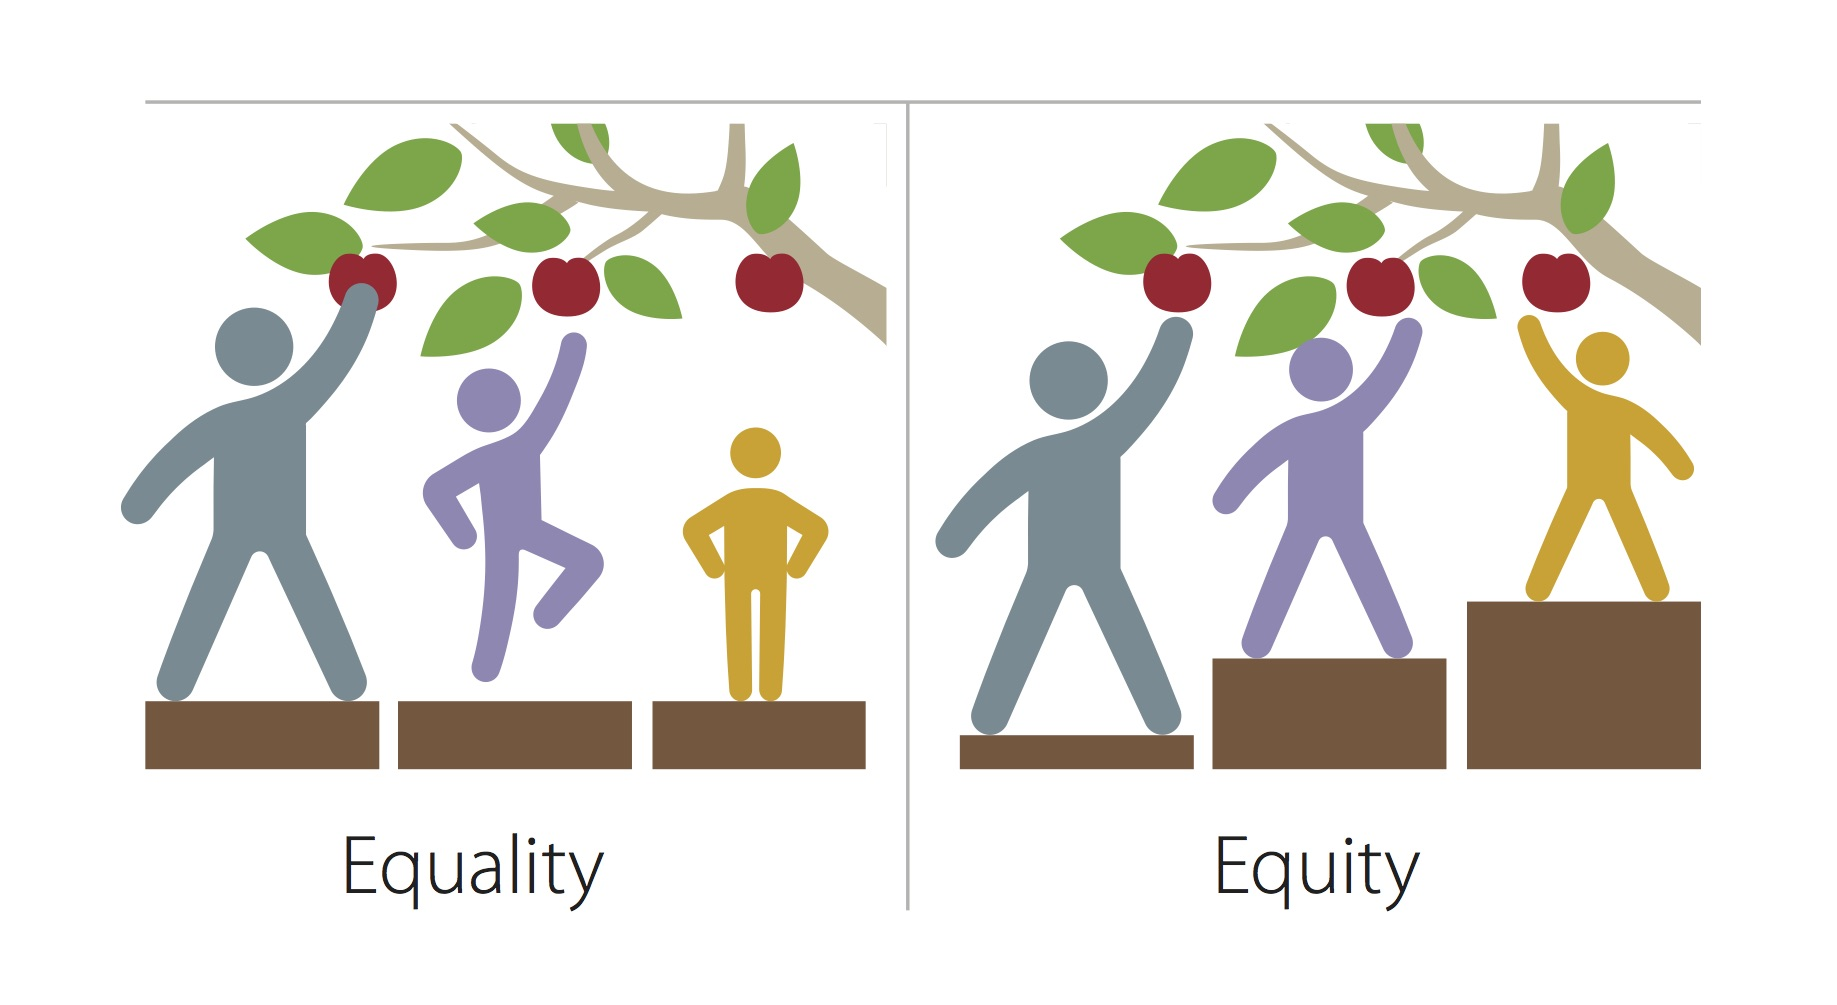
\includegraphics{assets/u6/Equity_vs_Equality.jpg}

\end{figure}%

\begin{tcolorbox}[enhanced jigsaw, toprule=.15mm, colback=white, colframe=quarto-callout-note-color-frame, arc=.35mm, opacityback=0, breakable, rightrule=.15mm, bottomrule=.15mm, leftrule=.75mm, left=2mm]
\begin{minipage}[t]{5.5mm}
\textcolor{quarto-callout-note-color}{\faInfo}
\end{minipage}%
\begin{minipage}[t]{\textwidth - 5.5mm}

\emph{Note}: From ``Equity vs Equality,'' by MPCA Photos, December 21,
2016, \emph{Flickr}
(\href{https://flickr.com/photos/mpcaphotos/31655988501/}{Equity vs
Equality \textbar{} MPCA Photos \textbar{} Flickr}).
\href{https://creativecommons.org/licenses/by-nc/2.0/}{CC BY-NC 2.0}.

\end{minipage}%
\end{tcolorbox}

DEI has been a hot topic for debate in recent years as organizations,
including universities, have emphasized DEI in the way they conduct
business, including hiring, promoting, and so on.

Let's take higher education as an example. As faculty members design
their courses, they consider the needs of their students and how to
effectively engage them in the course topics. They recognize the
diversity of students' needs and viewpoints and seek to create an
inclusive learning environment for students. Instructors might use
\href{https://udlguidelines.cast.org/}{Universal Design for Learning},
which is ``a framework \ldots{} to improve and optimize teaching and
learning for all people based on scientific insights into how humans
learn (CAST: UDL Guidelines, 2024, para. 1).''

Other teaching methods they might employ are
\href{https://www.facultyfocus.com/articles/equality-inclusion-and-diversity/five-essential-strategies-to-embrace-culturally-responsive-teaching/}{culturally
responsive teaching} (Singhal \& Gulati, 2020) or
\href{http://www.inclusioncanada.net/culturallyrelevantpedagogy.html}{culturally
relevant pedagogy} (Inclusion Canada, 2017)\emph{,} as a way to use
students' cultural experiences and perspectives as channels for
effective teaching and learning.

Key question: \emph{Should instructors treat all students the same
regardless of background, gender, beliefs, and so on?}

Many academics in higher education hold this value of equality. Others
promote equity, which ``takes into consideration a person's unique
circumstances, adjusting treatment accordingly so that the end result is
equal (McKinsey \& Company, 2022, Equity section).'' What does it mean
that the ``end result is equal?'' An equal opportunity to access and
succeed in academia? Or an equal outcome in which all students receive
the same grade?

This one example identifies one of the ``sticky points'' in the DEI
debate. In the next activity, we'll introduce some views on the DEI
topic.

\subsection{Activity: Perspectives on
DEI}\label{activity-perspectives-on-dei}

\begin{tcolorbox}[enhanced jigsaw, toprule=.15mm, colback=white, colframe=quarto-callout-note-color-frame, bottomtitle=1mm, leftrule=.75mm, coltitle=black, titlerule=0mm, rightrule=.15mm, colbacktitle=quarto-callout-note-color!10!white, left=2mm, title={Learning Activity}, opacitybacktitle=0.6, opacityback=0, breakable, toptitle=1mm, arc=.35mm, bottomrule=.15mm]

Here are a couple of contrasting points of view. If you choose to write
a social commentary on this topic be sure to explore various resources
with different opinions.

\begin{itemize}
\tightlist
\item
  \textbf{Read}:

  \begin{itemize}
  \tightlist
  \item
    \href{https://www.mckinsey.com/featured-insights/mckinsey-explainers/what-is-diversity-equity-and-inclusion}{What
    is Diversity, Equity, and Inclusion?} (2022)
  \item
    \href{https://www.theatlantic.com/ideas/archive/2023/07/hypocrisy-mandatory-diversity-statements/674611/}{The
    Hypocrisy of Mandatory Diversity Statements} (2023)
  \end{itemize}
\item
  \textbf{Watch}:
\item
  \href{https://www.youtube.com/watch?v=HR4wz1b54hw}{Diversity, Equity
  \& Inclusion. Learning How to Get it Right} (2023)
\end{itemize}

\url{https://www.youtube-nocookie.com/embed/HR4wz1b54hw}

\begin{itemize}
\tightlist
\item
  \href{https://www.youtube.com/watch?v=8WYi-64MejU}{Equity: The Thief
  of Human Potential} (2023)
\end{itemize}

\url{https://www.youtube-nocookie.com/embed/8WYi-64MejU}

\end{tcolorbox}

\subsection{Activity: DEI and Practising Christian
Hospitality}\label{activity-dei-and-practising-christian-hospitality}

\begin{tcolorbox}[enhanced jigsaw, toprule=.15mm, colback=white, colframe=quarto-callout-note-color-frame, bottomtitle=1mm, leftrule=.75mm, coltitle=black, titlerule=0mm, rightrule=.15mm, colbacktitle=quarto-callout-note-color!10!white, left=2mm, title={Learning Activity}, opacitybacktitle=0.6, opacityback=0, breakable, toptitle=1mm, arc=.35mm, bottomrule=.15mm]

As a final reflection on this topic, we invite you to read TWU's core
values page on
\href{https://www.twu.ca/about-us/commitments/core-values/practising-christian-hospitality}{\emph{Practising
Christian Hospitality}}.

TWU explains the core value of practising Christian hospitality:

\begin{quote}
Christian hospitality welcomes, genuinely includes and consistently
cares for \emph{all} individuals. Christ taught and modeled hospitality
to all, including those on the margins, as an essential element of
Christian faith and practice. Hospitality is vital to our life in the
Trinity Western University community and to our life in, and witness to,
other communities. \ldots{} Practising Christian hospitality undergirds
and promotes equity, diversity and inclusion.
\end{quote}

\textbf{Equity} is founded in our being created in the image of God;
every human being has inherent dignity and worth (Gen 1:26-28; 5:1-2;
Col 1:15).

\textbf{Diversity} is inherent in God's creation; it is good (Gen
1:11-12, 21-25).

\textbf{Inclusion} is essential to the body of Christ; we are diverse
and interdependent (1 Cor 12:12-31; Isa 56:3-8). (Trinity Western
University, n.d.-e)

As you read
\href{https://www.twu.ca/about-us/commitments/core-values/practising-christian-hospitality}{\emph{Practising
Christian Hospitality}}, consider the following questions, and how they
relate to your identity and actions online:

\begin{itemize}
\tightlist
\item
  How do we advocate for the dignity of all human beings and avoid any
  form of derogation or condescension?
\item
  How do we value the differences and diversity in God's creation?
\item
  How do we live peaceably and productively in society in the midst of
  enduring differences, even on very significant matters?
\item
  Does being inclusive demand agreement or consensus?
\item
  How can we practice Christian hospitality?
\end{itemize}

\end{tcolorbox}

We've explored a number of societal issues associated with the internet.
In the activity below, you will choose a topic of interest relating to
societal issues or problematic behaviours on the internet for further
investigation. You can select one of the topics introduced in this unit
or an alternate issue you find more interesting.

Here are few additional topics to consider:

\begin{itemize}
\tightlist
\item
  \href{https://computer.howstuffworks.com/10-forms-online-harassment.htm}{\emph{10
  Forms of Online Harassment}} (2015)
\item
  \href{https://karger.com/pps/article/86/3/129/282998/Cyberchondria-Challenges-of-Problematic-Online}{\emph{Cyberchondria}}
  (2017)
\item
  \href{https://www.bbc.com/news/technology-39371100}{\emph{The Woman
  Whose Phone `Misdiagnosed HIV'}} (2017) (complexities of mobile
  ownership in the developing world)
\item
  \href{https://www.theguardian.com/media/2017/mar/14/face-off-mps-and-social-media-giants-online-hate-speech-facebook-twitter}{\emph{Face-off
  Between MPs and Social Media Giants Over Online Hate Speech}} (2017)
  (hate speech online)
\item
  \href{https://en.wikipedia.org/wiki/Keystroke_logging}{\emph{Keystroke
  Logging}} (2024)
\item
  \href{https://theconversation.com/the-price-of-connection-surveillance-capitalism-64124}{\emph{The
  Price of Connection: Surveillance Capitalism}} (2016) (surveillance
  capitalism)
\item
  \emph{\href{https://hbr.org/2015/06/how-bots-took-over-twitter}{How
  Bots Took Over Twitter}} (2015) (bot problems)
\item
  \href{https://www.consumer.org.nz/articles/scams?gclid=EAIaIQobChMIrOzE7qX71AIVxBiPCh0uzAKrEAAYASAAEgIXf_D_BwE}{\emph{Scams
  and how to Avoid Them}} (n.d.)
\item
  \href{https://en.wikipedia.org/wiki/Fake_news}{\emph{Fake News}}
  (2024) 6.3.19 Activity: Editorial: Societal Issues on the Internet
\end{itemize}

\begin{tcolorbox}[enhanced jigsaw, toprule=.15mm, colback=white, colframe=quarto-callout-note-color-frame, bottomtitle=1mm, leftrule=.75mm, coltitle=black, titlerule=0mm, rightrule=.15mm, colbacktitle=quarto-callout-note-color!10!white, left=2mm, title={Learning Activity}, opacitybacktitle=0.6, opacityback=0, breakable, toptitle=1mm, arc=.35mm, bottomrule=.15mm]

\begin{itemize}
\tightlist
\item
  \textbf{Write}: Publish an editorial (400--600 words) on your blog on
  a societal issue or antisocial behaviour associated with the internet.
  Your editorial must:

  \begin{itemize}
  \tightlist
  \item
    Contain a minimum of four hyperlinks to supporting resources or
    issues. Your digital identity is connected to the internet and it is
    important to demonstrate how your contribution joins a networked
    conversation through connections in information.
  \item
    Include a representative image embedded in your blog post (n.b.,
    ensure that you have legal permission to use the image).
  \item
    If you are not sure about copyright, source a public domain image on
    a site such as \href{https://www.pexels.com/}{\emph{Pexels}}. Don't
    use sponsored or licensed images unless you have purchased the
    rights to use them.
  \item
    Include at least two references properly cited using APA style.
  \item
    Include a paragraph highlighting practical implications; for
    example, learning in a digital age or your current role.
  \end{itemize}
\end{itemize}

Remember to add a category or tag for your post using the course tag:
LDRS101.

\textbf{The Process:}

Choose a topic of interest.

\begin{itemize}
\tightlist
\item
  Conduct a search to identify reliable and credible online resources on
  your selected topic. Try to find resources from your own country or
  region, or your own area of work, and select the two best resources.
\item
  Read \href{https://www.wikihow.com/Write-a-Notable-Editorial}{How to
  Write a Notable Editorial} (2024).
\item
  Using the topic you selected, decide on the type of editorial to
  write, for example:

  \begin{itemize}
  \tightlist
  \item
    explaining or interpreting
  \item
    criticizing
  \item
    persuading
  \item
    praising
  \item
    Get your facts straight:
  \item
    revisit the online sources you identified previously
  \item
    search for additional resources if needed
  \end{itemize}
\item
  Prepare a thesis-like paragraph designed to catch the reader's
  attention and introduce what your editorial is about.
\item
  Prepare the body of your editorial providing an objective explanation
  of the issue supported by the relevant sources you have identified;
  for example:

  \begin{itemize}
  \tightlist
  \item
    state the opposing argument first
  \item
    present reasons refuting the opposition
  \item
    share your solutions
  \end{itemize}
\item
  Prepare a paragraph on practical implications, for instance, learning
  in a digital age or your current role.
\item
  Draft the conclusion.
\end{itemize}

\end{tcolorbox}

\section{Digital Wisdom}\label{digital-wisdom}

To conclude our course we will examine another perspective on ethics and
technology. This may tap into the foundational lens with which you
approach many ethical issues, so take a moment to reflect on the
following:

\begin{itemize}
\tightlist
\item
  What role does technology play in my social, academic, and spiritual
  life?
\item
  What guidance does the Bible have on our use of technology today?
\item
  How will my use of technology support my social, academic, and
  spiritual goals?
\end{itemize}

\subsection{Activity: Digital Wisdom}\label{activity-digital-wisdom}

\begin{tcolorbox}[enhanced jigsaw, toprule=.15mm, colback=white, colframe=quarto-callout-note-color-frame, bottomtitle=1mm, leftrule=.75mm, coltitle=black, titlerule=0mm, rightrule=.15mm, colbacktitle=quarto-callout-note-color!10!white, left=2mm, title={Learning Activity}, opacitybacktitle=0.6, opacityback=0, breakable, toptitle=1mm, arc=.35mm, bottomrule=.15mm]

\begin{itemize}
\tightlist
\item
  \textbf{Read}: Skim the following article in which the authors present
  a framework for digital wisdom, as well as practical practices that
  can help navigate the digital in our daily lives.

  \begin{itemize}
  \tightlist
  \item
    \href{https://christianscholars.com/a-framework-for-digital-wisdom-in-higher-education/}{\emph{A
    Framework for Digital Wisdom in Higher Education}} (2019).
  \end{itemize}
\end{itemize}

Here are some quotes that resonate (Paulus et al., 2019). Feel free to
highlight your quotes using Hypothes.is, or in your personal Obsidian
notes.

\begin{quote}
Institutions of higher education have a crucial role and responsibility
at this moment of technological change to form people who will flourish
in our so-called digital age. (2019, para. 1)

Within the context of Christian higher education, the need to integrate
new ICTs into our individual and institutional lives well and
wisely---as we consider what technologies are doing to us and what we
will do with them---is of utmost significance if we are committed to the
cultivation of competence, character, and wisdom. (2019, para. 6)

Scripture enables us look behind and beyond our and others' online
identities to see ourselves and others as embodied and relational beings
made in the image of God. (2019, para. 21)

Our use of technologies must be shaped by our intentions and values, and
we must be aware of how platform interfaces, permissions, algorithms,
and other design elements could interfere with our goals and
obligations. (2019, para. 31)
\end{quote}

\textbf{Questions to Consider}

Answer the following questions in your journal:

\begin{itemize}
\tightlist
\item
  How can you, as a TWU student, flourish in this digital age?
\item
  How do the tools you use shape you? How do you use them wisely?
\item
  How should we view and relate to others online---in particular those
  whom we disagree with?
\item
  How can you cultivate inclusive digital communities which embody a
  sense of belonging, connection, and Christian hospitality?
\item
  And finally, how can we use technology in a way that aligns with our
  intentions and values?
\end{itemize}

\end{tcolorbox}

\section{Summary}\label{summary-5}

As you complete this course and continue on your learning journey we
trust that you have acquired skills that will not only prepare you for
your academic studies but also for your professional goals.

We began this final unit by emphasizing the value of community in online
learning. Throughout the course we have encouraged you to connect with
others---fellow TWU students, instructors, colleagues, family, friends,
and other online communities. Reflect on how these connections have
influenced your learning experience. Additionally, we discussed the
impact of technology in the workplace and how you might use tools
effectively in your business practices or field of study. You have had
opportunities to engage as global digital citizens by using technology
to discover and share knowledge. Furthermore, we examined emerging
societal issues and online behaviours, discussing strategies to address
these challenges effectively.

Finally, we introduced the concept of digital wisdom. As you continue to
integrate technology into your learning journey, we encourage you to
consider how your online contributions can positively impact others.
Reflect on TWU's mission and vision statements and how they resonate
with you and guide your commitment to serving others and glorifying God.

\begin{quote}
The mission of Trinity Western University, as an arm of the Church, is
to develop godly Christian leaders: positive, goal-oriented university
graduates with thoroughly Christian minds; growing disciples of Jesus
Christ who glorify God through fulfilling the Great Commission, serving
God and people in the various marketplaces of life.

Every graduate is equipped to think truthfully, act justly, and live
faithfully for the good of the world and the glory of God. (Trinity
Western University, n.d.-d)
\end{quote}

\begin{tcolorbox}[enhanced jigsaw, toprule=.15mm, colback=white, colframe=quarto-callout-note-color-frame, bottomtitle=1mm, leftrule=.75mm, coltitle=black, titlerule=0mm, rightrule=.15mm, colbacktitle=quarto-callout-note-color!10!white, left=2mm, title={Checking Your Learning}, opacitybacktitle=0.6, opacityback=0, breakable, toptitle=1mm, arc=.35mm, bottomrule=.15mm]

Before you move on to the next unit check that you are able to:

\begin{itemize}
\tightlist
\item
  Discuss how technology has changed business practices in your field of
  interest or career
\item
  Utilize technology to discover and share knowledge, collaborate with
  others, and become engaged digital global citizens
\item
  Describe societal issues and problematic online behaviours which have
  emerged in the digital world and how to deal with these challenges in
  an ethical manner
\item
  Create inclusive digital communities which embody a sense of
  belonging, connection, and Christian hospitality
\item
  Create a personalized narrative to document and express your learning
  process
\item
  Practice evaluative judgment to document your process of learning in
  complex domains of knowledge
\end{itemize}

\end{tcolorbox}




\end{document}
